% Options for packages loaded elsewhere
\PassOptionsToPackage{unicode}{hyperref}
\PassOptionsToPackage{hyphens}{url}
\PassOptionsToPackage{dvipsnames,svgnames,x11names}{xcolor}
%
\documentclass[
  letterpaper,
  DIV=11,
  numbers=noendperiod]{scrreprt}

\usepackage{amsmath,amssymb}
\usepackage{lmodern}
\usepackage{iftex}
\ifPDFTeX
  \usepackage[T1]{fontenc}
  \usepackage[utf8]{inputenc}
  \usepackage{textcomp} % provide euro and other symbols
\else % if luatex or xetex
  \usepackage{unicode-math}
  \defaultfontfeatures{Scale=MatchLowercase}
  \defaultfontfeatures[\rmfamily]{Ligatures=TeX,Scale=1}
\fi
% Use upquote if available, for straight quotes in verbatim environments
\IfFileExists{upquote.sty}{\usepackage{upquote}}{}
\IfFileExists{microtype.sty}{% use microtype if available
  \usepackage[]{microtype}
  \UseMicrotypeSet[protrusion]{basicmath} % disable protrusion for tt fonts
}{}
\makeatletter
\@ifundefined{KOMAClassName}{% if non-KOMA class
  \IfFileExists{parskip.sty}{%
    \usepackage{parskip}
  }{% else
    \setlength{\parindent}{0pt}
    \setlength{\parskip}{6pt plus 2pt minus 1pt}}
}{% if KOMA class
  \KOMAoptions{parskip=half}}
\makeatother
\usepackage{xcolor}
\setlength{\emergencystretch}{3em} % prevent overfull lines
\setcounter{secnumdepth}{5}
% Make \paragraph and \subparagraph free-standing
\ifx\paragraph\undefined\else
  \let\oldparagraph\paragraph
  \renewcommand{\paragraph}[1]{\oldparagraph{#1}\mbox{}}
\fi
\ifx\subparagraph\undefined\else
  \let\oldsubparagraph\subparagraph
  \renewcommand{\subparagraph}[1]{\oldsubparagraph{#1}\mbox{}}
\fi

\usepackage{color}
\usepackage{fancyvrb}
\newcommand{\VerbBar}{|}
\newcommand{\VERB}{\Verb[commandchars=\\\{\}]}
\DefineVerbatimEnvironment{Highlighting}{Verbatim}{commandchars=\\\{\}}
% Add ',fontsize=\small' for more characters per line
\usepackage{framed}
\definecolor{shadecolor}{RGB}{241,243,245}
\newenvironment{Shaded}{\begin{snugshade}}{\end{snugshade}}
\newcommand{\AlertTok}[1]{\textcolor[rgb]{0.68,0.00,0.00}{#1}}
\newcommand{\AnnotationTok}[1]{\textcolor[rgb]{0.37,0.37,0.37}{#1}}
\newcommand{\AttributeTok}[1]{\textcolor[rgb]{0.40,0.45,0.13}{#1}}
\newcommand{\BaseNTok}[1]{\textcolor[rgb]{0.68,0.00,0.00}{#1}}
\newcommand{\BuiltInTok}[1]{\textcolor[rgb]{0.00,0.23,0.31}{#1}}
\newcommand{\CharTok}[1]{\textcolor[rgb]{0.13,0.47,0.30}{#1}}
\newcommand{\CommentTok}[1]{\textcolor[rgb]{0.37,0.37,0.37}{#1}}
\newcommand{\CommentVarTok}[1]{\textcolor[rgb]{0.37,0.37,0.37}{\textit{#1}}}
\newcommand{\ConstantTok}[1]{\textcolor[rgb]{0.56,0.35,0.01}{#1}}
\newcommand{\ControlFlowTok}[1]{\textcolor[rgb]{0.00,0.23,0.31}{#1}}
\newcommand{\DataTypeTok}[1]{\textcolor[rgb]{0.68,0.00,0.00}{#1}}
\newcommand{\DecValTok}[1]{\textcolor[rgb]{0.68,0.00,0.00}{#1}}
\newcommand{\DocumentationTok}[1]{\textcolor[rgb]{0.37,0.37,0.37}{\textit{#1}}}
\newcommand{\ErrorTok}[1]{\textcolor[rgb]{0.68,0.00,0.00}{#1}}
\newcommand{\ExtensionTok}[1]{\textcolor[rgb]{0.00,0.23,0.31}{#1}}
\newcommand{\FloatTok}[1]{\textcolor[rgb]{0.68,0.00,0.00}{#1}}
\newcommand{\FunctionTok}[1]{\textcolor[rgb]{0.28,0.35,0.67}{#1}}
\newcommand{\ImportTok}[1]{\textcolor[rgb]{0.00,0.46,0.62}{#1}}
\newcommand{\InformationTok}[1]{\textcolor[rgb]{0.37,0.37,0.37}{#1}}
\newcommand{\KeywordTok}[1]{\textcolor[rgb]{0.00,0.23,0.31}{#1}}
\newcommand{\NormalTok}[1]{\textcolor[rgb]{0.00,0.23,0.31}{#1}}
\newcommand{\OperatorTok}[1]{\textcolor[rgb]{0.37,0.37,0.37}{#1}}
\newcommand{\OtherTok}[1]{\textcolor[rgb]{0.00,0.23,0.31}{#1}}
\newcommand{\PreprocessorTok}[1]{\textcolor[rgb]{0.68,0.00,0.00}{#1}}
\newcommand{\RegionMarkerTok}[1]{\textcolor[rgb]{0.00,0.23,0.31}{#1}}
\newcommand{\SpecialCharTok}[1]{\textcolor[rgb]{0.37,0.37,0.37}{#1}}
\newcommand{\SpecialStringTok}[1]{\textcolor[rgb]{0.13,0.47,0.30}{#1}}
\newcommand{\StringTok}[1]{\textcolor[rgb]{0.13,0.47,0.30}{#1}}
\newcommand{\VariableTok}[1]{\textcolor[rgb]{0.07,0.07,0.07}{#1}}
\newcommand{\VerbatimStringTok}[1]{\textcolor[rgb]{0.13,0.47,0.30}{#1}}
\newcommand{\WarningTok}[1]{\textcolor[rgb]{0.37,0.37,0.37}{\textit{#1}}}

\providecommand{\tightlist}{%
  \setlength{\itemsep}{0pt}\setlength{\parskip}{0pt}}\usepackage{longtable,booktabs,array}
\usepackage{calc} % for calculating minipage widths
% Correct order of tables after \paragraph or \subparagraph
\usepackage{etoolbox}
\makeatletter
\patchcmd\longtable{\par}{\if@noskipsec\mbox{}\fi\par}{}{}
\makeatother
% Allow footnotes in longtable head/foot
\IfFileExists{footnotehyper.sty}{\usepackage{footnotehyper}}{\usepackage{footnote}}
\makesavenoteenv{longtable}
\usepackage{graphicx}
\makeatletter
\def\maxwidth{\ifdim\Gin@nat@width>\linewidth\linewidth\else\Gin@nat@width\fi}
\def\maxheight{\ifdim\Gin@nat@height>\textheight\textheight\else\Gin@nat@height\fi}
\makeatother
% Scale images if necessary, so that they will not overflow the page
% margins by default, and it is still possible to overwrite the defaults
% using explicit options in \includegraphics[width, height, ...]{}
\setkeys{Gin}{width=\maxwidth,height=\maxheight,keepaspectratio}
% Set default figure placement to htbp
\makeatletter
\def\fps@figure{htbp}
\makeatother
\newlength{\cslhangindent}
\setlength{\cslhangindent}{1.5em}
\newlength{\csllabelwidth}
\setlength{\csllabelwidth}{3em}
\newlength{\cslentryspacingunit} % times entry-spacing
\setlength{\cslentryspacingunit}{\parskip}
\newenvironment{CSLReferences}[2] % #1 hanging-ident, #2 entry spacing
 {% don't indent paragraphs
  \setlength{\parindent}{0pt}
  % turn on hanging indent if param 1 is 1
  \ifodd #1
  \let\oldpar\par
  \def\par{\hangindent=\cslhangindent\oldpar}
  \fi
  % set entry spacing
  \setlength{\parskip}{#2\cslentryspacingunit}
 }%
 {}
\usepackage{calc}
\newcommand{\CSLBlock}[1]{#1\hfill\break}
\newcommand{\CSLLeftMargin}[1]{\parbox[t]{\csllabelwidth}{#1}}
\newcommand{\CSLRightInline}[1]{\parbox[t]{\linewidth - \csllabelwidth}{#1}\break}
\newcommand{\CSLIndent}[1]{\hspace{\cslhangindent}#1}

\usepackage{booktabs}
\usepackage{caption}
\usepackage{longtable}
\KOMAoption{captions}{tableheading}
\makeatletter
\makeatother
\makeatletter
\@ifpackageloaded{bookmark}{}{\usepackage{bookmark}}
\makeatother
\makeatletter
\@ifpackageloaded{caption}{}{\usepackage{caption}}
\AtBeginDocument{%
\ifdefined\contentsname
  \renewcommand*\contentsname{Table of contents}
\else
  \newcommand\contentsname{Table of contents}
\fi
\ifdefined\listfigurename
  \renewcommand*\listfigurename{List of Figures}
\else
  \newcommand\listfigurename{List of Figures}
\fi
\ifdefined\listtablename
  \renewcommand*\listtablename{List of Tables}
\else
  \newcommand\listtablename{List of Tables}
\fi
\ifdefined\figurename
  \renewcommand*\figurename{Figure}
\else
  \newcommand\figurename{Figure}
\fi
\ifdefined\tablename
  \renewcommand*\tablename{Table}
\else
  \newcommand\tablename{Table}
\fi
}
\@ifpackageloaded{float}{}{\usepackage{float}}
\floatstyle{ruled}
\@ifundefined{c@chapter}{\newfloat{codelisting}{h}{lop}}{\newfloat{codelisting}{h}{lop}[chapter]}
\floatname{codelisting}{Listing}
\newcommand*\listoflistings{\listof{codelisting}{List of Listings}}
\makeatother
\makeatletter
\@ifpackageloaded{caption}{}{\usepackage{caption}}
\@ifpackageloaded{subcaption}{}{\usepackage{subcaption}}
\makeatother
\makeatletter
\@ifpackageloaded{tcolorbox}{}{\usepackage[many]{tcolorbox}}
\makeatother
\makeatletter
\@ifundefined{shadecolor}{\definecolor{shadecolor}{rgb}{.97, .97, .97}}
\makeatother
\makeatletter
\makeatother
\ifLuaTeX
  \usepackage{selnolig}  % disable illegal ligatures
\fi
\IfFileExists{bookmark.sty}{\usepackage{bookmark}}{\usepackage{hyperref}}
\IfFileExists{xurl.sty}{\usepackage{xurl}}{} % add URL line breaks if available
\urlstyle{same} % disable monospaced font for URLs
\hypersetup{
  pdftitle={Latent Variable Modelling Workflow Reference},
  pdfauthor={Alex Rand},
  colorlinks=true,
  linkcolor={blue},
  filecolor={Maroon},
  citecolor={Blue},
  urlcolor={Blue},
  pdfcreator={LaTeX via pandoc}}

\title{Latent Variable Modelling Workflow Reference}
\author{Alex Rand}
\date{10/25/2022}

\begin{document}
\maketitle
\ifdefined\Shaded\renewenvironment{Shaded}{\begin{tcolorbox}[sharp corners, frame hidden, enhanced, borderline west={3pt}{0pt}{shadecolor}, boxrule=0pt, breakable, interior hidden]}{\end{tcolorbox}}\fi

\renewcommand*\contentsname{Table of contents}
{
\hypersetup{linkcolor=}
\setcounter{tocdepth}{2}
\tableofcontents
}
\bookmarksetup{startatroot}

\hypertarget{preface}{%
\chapter*{Preface}\label{preface}}
\addcontentsline{toc}{chapter}{Preface}

\hypertarget{what-is-this}{%
\section*{What is this?}\label{what-is-this}}
\addcontentsline{toc}{section}{What is this?}

This document does two things:

\begin{enumerate}
\def\labelenumi{\arabic{enumi}.}
\tightlist
\item
  Give a conceptual overview of latent variable modelling, especially
  confirmatory factor analysis (CFA).
\item
  Provide workflows I've cobbled together from a few different
  textbooks, including examples with data from those textbooks or from
  open datasets I found online.
\end{enumerate}

\hypertarget{what-am-i-referencing}{%
\section*{What am I referencing?}\label{what-am-i-referencing}}
\addcontentsline{toc}{section}{What am I referencing?}

The first book on latent variable modelling I read was Gorsuch (1983).
This was a nice conceptual introduction, but the applied examples
weren't great. I've since found a few sources with data and R code to
work with. I also cite these sources throughout as I cobble together the
workflows.

\begin{itemize}
\item
  \href{https://www.routledge.com/Latent-Variable-Modeling-with-R/Finch-French/p/book/9780415832458}{\emph{Latent
  Variable Modelling with R}}, by Finch (2015). They helpfully provide
  all of the datasets
  \href{https://www.routledge.com/Latent-Variable-Modeling-with-R/Finch-French/p/book/9780415832458}{here}.
\item
  \href{https://www.guilford.com/books/Principles-and-Practice-of-Structural-Equation-Modeling/Rex-Kline/9781462523344}{\emph{Principles
  and Practice of Structural Equation Modeling}}, by Kline (2011). The
  publisher provides data and code
  \href{https://www.guilford.com/companion-site/Principles-and-Practice-of-Structural-Equation-Modeling-Fourth-Edition/9781462523344}{here}.
\item
  \href{http://www.kharazmi-statistics.ir/Uploads/Public/book/Methodology\%20in\%20the\%20Social\%20Sciences.pdf}{Confirmatory
  Factor Analysis for Applied Research}, by Brown (2006). No R code
  available, but there's some data at
  \href{https://people.bu.edu/tabrown/cfabook.html}{the university
  website}
\item
  \href{https://www.usgs.gov/centers/wetland-and-aquatic-research-center/science/quantitative-analysis-using-structural-equation}{Quantitative
  Analysis Using Structural Equation Modelling}, a free online course
  provided by the Wetland and Aquatic Research Center of the United
  States Geological Survey.
\item
  \href{https://www.lavaan.ugent.be/tutorial/index.html}{The
  \emph{lavaan} documentation} has some nice worked examples too.
\end{itemize}

I'll mostly be using \textbf{lavaan} and \textbf{tidyverse}, but maybe
also some \textbf{brms} at some point.

\part{Introduction to CFA}

\begin{Shaded}
\begin{Highlighting}[]
\FunctionTok{library}\NormalTok{(tidyverse)}
\FunctionTok{library}\NormalTok{(ggdag)}
\end{Highlighting}
\end{Shaded}

\hypertarget{the-whole-game}{%
\section*{The Whole Game}\label{the-whole-game}}
\addcontentsline{toc}{section}{The Whole Game}

The Whole Game of Confirmatory Factor Analysis (CFA) is that I'm trying
to convince you my observed variables are confounded by some unmeasured
variables. Usually I'm trying to show that the observed ariables are
confounded in a very particular way, where a few small groups of
variables are confounded only by one unmeasured variable per group.

So here's the archetypal DAG of a CFA, where the Xs are observed
variables, and F1 is an unmeasured variable I am trying to convince you
exists. We can call this \textbf{The Primordial CFA DAG}:

\begin{Shaded}
\begin{Highlighting}[]
\CommentTok{\# Set DAG coordinates}
\NormalTok{dag\_coords }\OtherTok{\textless{}{-}} \FunctionTok{list}\NormalTok{(}
  \AttributeTok{x =} \FunctionTok{c}\NormalTok{(}
    \AttributeTok{F1 =} \DecValTok{1}\NormalTok{, }
    \AttributeTok{X1 =} \DecValTok{2}\NormalTok{,}
    \AttributeTok{X2 =} \DecValTok{2}\NormalTok{,}
    \AttributeTok{X3 =} \DecValTok{2}
\NormalTok{  ),}
  \AttributeTok{y =} \FunctionTok{c}\NormalTok{(}
    \AttributeTok{F1 =} \FloatTok{1.5}\NormalTok{,}
    \AttributeTok{X1 =} \FloatTok{1.8}\NormalTok{,}
    \AttributeTok{X2 =} \FloatTok{1.5}\NormalTok{,}
    \AttributeTok{X3 =} \FloatTok{1.2}
\NormalTok{  )}
\NormalTok{)}

\CommentTok{\# Set DAG relationships and aesthetics}
\NormalTok{measurement\_confounding\_dag }\OtherTok{\textless{}{-}}\NormalTok{ ggdag}\SpecialCharTok{::}\FunctionTok{dagify}\NormalTok{(}
\NormalTok{  X1 }\SpecialCharTok{\textasciitilde{}}\NormalTok{ F1,}
\NormalTok{  X2 }\SpecialCharTok{\textasciitilde{}}\NormalTok{ F1,}
\NormalTok{  X3 }\SpecialCharTok{\textasciitilde{}}\NormalTok{ F1,}
  \AttributeTok{coords =}\NormalTok{ dag\_coords}
\NormalTok{) }\SpecialCharTok{\%\textgreater{}\%} 
  
  \FunctionTok{tidy\_dagitty}\NormalTok{() }\SpecialCharTok{\%\textgreater{}\%} 
  
  \FunctionTok{mutate}\NormalTok{(}
    \StringTok{\textasciigrave{}}\AttributeTok{ }\StringTok{\textasciigrave{}} \OtherTok{=} \FunctionTok{case\_when}\NormalTok{(}
      \FunctionTok{grepl}\NormalTok{(}\StringTok{"\^{}F"}\NormalTok{, name) }\SpecialCharTok{\textasciitilde{}} \StringTok{"latent"}\NormalTok{,}
      \FunctionTok{grepl}\NormalTok{(}\StringTok{"\^{}X"}\NormalTok{, name) }\SpecialCharTok{\textasciitilde{}} \StringTok{"observed"}
\NormalTok{    ))}

\CommentTok{\# Plot the DAG}
\NormalTok{measurement\_confounding\_dag }\SpecialCharTok{\%\textgreater{}\%}
  \FunctionTok{ggplot}\NormalTok{(}\FunctionTok{aes}\NormalTok{(}\AttributeTok{x =}\NormalTok{ x, }\AttributeTok{y =}\NormalTok{ y, }\AttributeTok{xend =}\NormalTok{ xend, }\AttributeTok{yend =}\NormalTok{ yend)) }\SpecialCharTok{+}
  \FunctionTok{geom\_dag\_point}\NormalTok{(}\FunctionTok{aes}\NormalTok{(}\AttributeTok{colour =} \StringTok{\textasciigrave{}}\AttributeTok{ }\StringTok{\textasciigrave{}}\NormalTok{)) }\SpecialCharTok{+}
  \FunctionTok{scale\_colour\_manual}\NormalTok{(}\AttributeTok{values =} \FunctionTok{c}\NormalTok{(}\StringTok{"dark blue"}\NormalTok{, }\StringTok{"\#edbc64"}\NormalTok{)) }\SpecialCharTok{+} 
  \FunctionTok{geom\_dag\_edges}\NormalTok{() }\SpecialCharTok{+}
  \FunctionTok{geom\_dag\_text}\NormalTok{() }\SpecialCharTok{+}
  \FunctionTok{theme}\NormalTok{(}\AttributeTok{legend.title =} \FunctionTok{element\_blank}\NormalTok{()) }\SpecialCharTok{+}
  \FunctionTok{theme\_void}\NormalTok{()}
\end{Highlighting}
\end{Shaded}

\begin{figure}[H]

{\centering 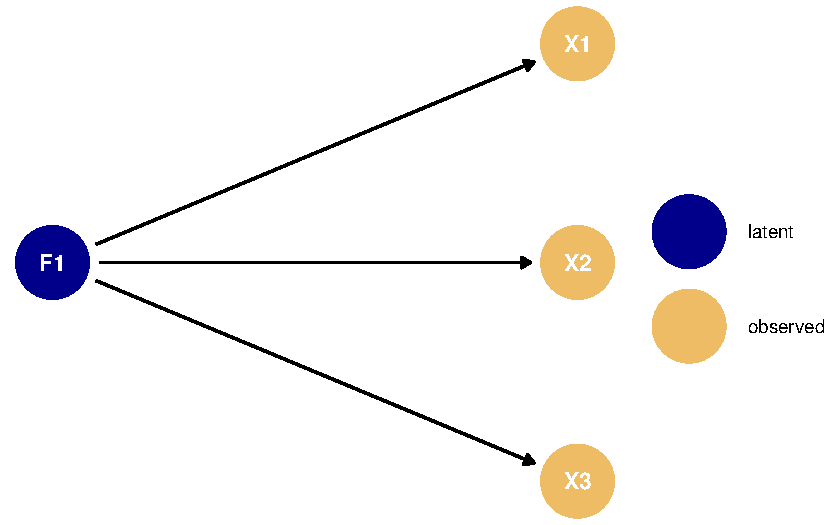
\includegraphics{./cfa-intro_files/figure-pdf/unnamed-chunk-2-1.pdf}

}

\end{figure}

CFA is just a way of trying to see whether the patterns of variance and
covariance in your data are consistent with the above DAG, or a similar
one.

The classic way of testing whether your data are consistent with a DAG
is to condition on some of the variables, perhaps by including it as a
predictor in a linear regression model, and see whether the patterns of
correlation change in the ways the DAG expects based on the rules of
d-separation. For the above DAG, this would mean controlling for F1 and
seeing whether the correlations between X1, X2, and X3 decrease as a
result. But in CFA we always assume the confounder is unmeasured, so we
can't directly control for it. Instead, we can only try to argue for our
DAG in a more hand-wavy sort of way: we expect confounded variables to
be correlated with each other, and uncounfounded variables to \emph{not}
be correlated with each other. This is why we focus on the empirical
correlation matrix as the basis for our model: if a few of my variables
are very correlated with each other then that is \emph{consistent} with
them being confounded by the same unobserved variable. But it is not
proof! You can never prove a DAG, after all.

So interpreting a CFA model is all about checking to see whether the
correlations between the variables are consistent with what we would
expect to see under the DAG where each group of variables is confounded
by a single unmeasured variable. In the next few chapters we'll look at
some examples of how people have liked to make the case for their
unmeasured-confounder DAG.

\hypertarget{sec-basic-workflow}{%
\chapter{Traditional CFA Workflow}\label{sec-basic-workflow}}

\begin{Shaded}
\begin{Highlighting}[]
\FunctionTok{library}\NormalTok{(tidyverse)}
\FunctionTok{library}\NormalTok{(lavaan)}
\FunctionTok{library}\NormalTok{(ggdag)}
\end{Highlighting}
\end{Shaded}

\hypertarget{example-1-toxic-striving-energy}{%
\section*{Example 1: Toxic Striving
Energy}\label{example-1-toxic-striving-energy}}
\addcontentsline{toc}{section}{Example 1: Toxic Striving Energy}

The first example we'll look at is from Finch (2015), chapter 3. The
practice dataset is introduced on page 10. It is from a study about
human motivation. The dataset is a weird questionnaire called the
`Achievement Goal Scale' (AGS), which asks people 12 questions about how
much toxic striving energy they have. The dataset provided seems to have
lots of mysterious columns in it, but we're probably good to just keep
the columns with responses to the AGS questionnaire:

\begin{Shaded}
\begin{Highlighting}[]
\DocumentationTok{\#\#\# Load the data}
\NormalTok{dat\_raw }\OtherTok{\textless{}{-}}\NormalTok{ foreign}\SpecialCharTok{::}\FunctionTok{read.spss}\NormalTok{(}\StringTok{\textquotesingle{}../data/finch{-}and{-}french/edps744.sav\textquotesingle{}}\NormalTok{) }
  
\DocumentationTok{\#\#\# Clean the data}
\NormalTok{dat\_ags }\OtherTok{\textless{}{-}}\NormalTok{ dat\_raw }\SpecialCharTok{\%\textgreater{}\%} 

  \CommentTok{\# Convert to a data frame for ease of use}
  \FunctionTok{as.data.frame}\NormalTok{() }\SpecialCharTok{\%\textgreater{}\%} 
  
  \CommentTok{\# Keep only columns that start with the prefix \textquotesingle{}ags\textquotesingle{} followed by a question number}
  \FunctionTok{select}\NormalTok{(}\FunctionTok{matches}\NormalTok{(}\StringTok{"ags}\SpecialCharTok{\textbackslash{}\textbackslash{}}\StringTok{d"}\NormalTok{)) }
\end{Highlighting}
\end{Shaded}

\hypertarget{data-exploration}{%
\subsection*{Data Exploration}\label{data-exploration}}
\addcontentsline{toc}{subsection}{Data Exploration}

We don't want to do too much exploration before fitting our factor
models, because the whole game of CFA is to commit to our hypotheses
before checking what the data looks like, so we don't mislead ourselves
with
\href{http://www.stat.columbia.edu/~gelman/research/unpublished/p_hacking.pdf}{forking
paths}. But just for fun, we can explore the distributions of the
answers to each of the 12 questions:

\begin{Shaded}
\begin{Highlighting}[]
\NormalTok{dat\_ags }\SpecialCharTok{\%\textgreater{}\%} 

  \CommentTok{\# Pivot to prepare the data for visualization}
  \FunctionTok{pivot\_longer}\NormalTok{(}
    \AttributeTok{cols      =} \FunctionTok{everything}\NormalTok{(),}
    \AttributeTok{names\_to  =} \StringTok{"question"}\NormalTok{,}
    \AttributeTok{values\_to =} \StringTok{"response"}\NormalTok{,}
    \AttributeTok{names\_transform =} \FunctionTok{list}\NormalTok{(}\AttributeTok{question =}\NormalTok{ fct\_inorder)  }
\NormalTok{  ) }\SpecialCharTok{\%\textgreater{}\%} 

  \CommentTok{\# Plot}
  \FunctionTok{ggplot}\NormalTok{() }\SpecialCharTok{+}
  \FunctionTok{geom\_histogram}\NormalTok{(}\FunctionTok{aes}\NormalTok{(}\AttributeTok{x =}\NormalTok{ response)) }\SpecialCharTok{+} 
  \FunctionTok{theme\_bw}\NormalTok{() }\SpecialCharTok{+} 
  \FunctionTok{facet\_wrap}\NormalTok{(}\SpecialCharTok{\textasciitilde{}}\NormalTok{question)}
\end{Highlighting}
\end{Shaded}

\begin{figure}[H]

{\centering 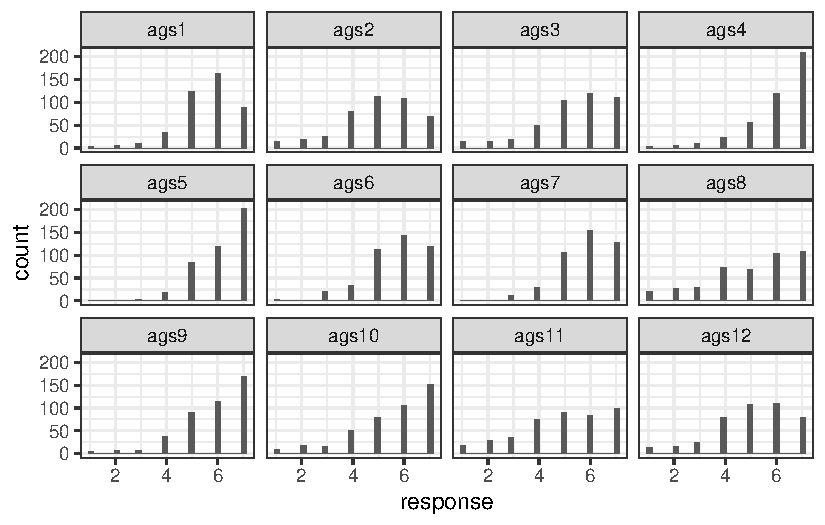
\includegraphics{./traditional-cfa-workflow_files/figure-pdf/unnamed-chunk-3-1.pdf}

}

\end{figure}

Seems like some questions have different means and variances from each
other. For example, the answers to \texttt{ags11} and \texttt{ags12} are
relatively flat, while the answers to \texttt{ags4} and \texttt{ags5}
are more bunched up around the highest values. The responses clearly
skew towards higher values in aggregate.

We can also do some healthy exploration of missingness in the dataset.
For starters: what proportion of values are missing in each row?

\begin{Shaded}
\begin{Highlighting}[]
\NormalTok{dat\_ags }\SpecialCharTok{\%\textgreater{}\%} 
  
  \CommentTok{\# Calculate the proportion of missing values }
  \FunctionTok{summarise\_all}\NormalTok{(}\SpecialCharTok{\textasciitilde{}} \FunctionTok{sum}\NormalTok{(}\FunctionTok{is.na}\NormalTok{(.)) }\SpecialCharTok{/}\NormalTok{ (}\FunctionTok{sum}\NormalTok{(}\FunctionTok{is.na}\NormalTok{(.) }\SpecialCharTok{+} \FunctionTok{sum}\NormalTok{(}\SpecialCharTok{!}\FunctionTok{is.na}\NormalTok{(.))))) }\SpecialCharTok{\%\textgreater{}\%} 
  
  \CommentTok{\# Rounding to make the results more presentable}
  \FunctionTok{mutate}\NormalTok{(}\FunctionTok{across}\NormalTok{(}\FunctionTok{everything}\NormalTok{(), round, }\DecValTok{6}\NormalTok{)) }\SpecialCharTok{\%\textgreater{}\%} 
  
  \CommentTok{\# Create the table}
\NormalTok{  knitr}\SpecialCharTok{::}\FunctionTok{kable}\NormalTok{(}\AttributeTok{title =} \StringTok{"Proportion of Missing Responses in Each Column"}\NormalTok{) }
\end{Highlighting}
\end{Shaded}

\begin{verbatim}
Warning: There was 1 warning in `mutate()`.
i In argument: `across(everything(), round, 6)`.
Caused by warning:
! The `...` argument of `across()` is deprecated as of dplyr 1.1.0.
Supply arguments directly to `.fns` through an anonymous function instead.

  # Previously
  across(a:b, mean, na.rm = TRUE)

  # Now
  across(a:b, \(x) mean(x, na.rm = TRUE))
\end{verbatim}

\begin{longtable}[]{@{}
  >{\raggedleft\arraybackslash}p{(\columnwidth - 22\tabcolsep) * \real{0.0870}}
  >{\raggedleft\arraybackslash}p{(\columnwidth - 22\tabcolsep) * \real{0.0652}}
  >{\raggedleft\arraybackslash}p{(\columnwidth - 22\tabcolsep) * \real{0.0652}}
  >{\raggedleft\arraybackslash}p{(\columnwidth - 22\tabcolsep) * \real{0.0870}}
  >{\raggedleft\arraybackslash}p{(\columnwidth - 22\tabcolsep) * \real{0.0870}}
  >{\raggedleft\arraybackslash}p{(\columnwidth - 22\tabcolsep) * \real{0.0870}}
  >{\raggedleft\arraybackslash}p{(\columnwidth - 22\tabcolsep) * \real{0.0870}}
  >{\raggedleft\arraybackslash}p{(\columnwidth - 22\tabcolsep) * \real{0.0870}}
  >{\raggedleft\arraybackslash}p{(\columnwidth - 22\tabcolsep) * \real{0.0870}}
  >{\raggedleft\arraybackslash}p{(\columnwidth - 22\tabcolsep) * \real{0.0870}}
  >{\raggedleft\arraybackslash}p{(\columnwidth - 22\tabcolsep) * \real{0.0870}}
  >{\raggedleft\arraybackslash}p{(\columnwidth - 22\tabcolsep) * \real{0.0870}}@{}}
\toprule()
\begin{minipage}[b]{\linewidth}\raggedleft
ags1
\end{minipage} & \begin{minipage}[b]{\linewidth}\raggedleft
ags2
\end{minipage} & \begin{minipage}[b]{\linewidth}\raggedleft
ags3
\end{minipage} & \begin{minipage}[b]{\linewidth}\raggedleft
ags4
\end{minipage} & \begin{minipage}[b]{\linewidth}\raggedleft
ags5
\end{minipage} & \begin{minipage}[b]{\linewidth}\raggedleft
ags6
\end{minipage} & \begin{minipage}[b]{\linewidth}\raggedleft
ags7
\end{minipage} & \begin{minipage}[b]{\linewidth}\raggedleft
ags8
\end{minipage} & \begin{minipage}[b]{\linewidth}\raggedleft
ags9
\end{minipage} & \begin{minipage}[b]{\linewidth}\raggedleft
ags10
\end{minipage} & \begin{minipage}[b]{\linewidth}\raggedleft
ags11
\end{minipage} & \begin{minipage}[b]{\linewidth}\raggedleft
ags12
\end{minipage} \\
\midrule()
\endhead
1.1e-05 & 5e-06 & 5e-06 & 1.6e-05 & 1.6e-05 & 1.1e-05 & 1.6e-05 &
1.6e-05 & 1.1e-05 & 2.2e-05 & 1.1e-05 & 1.6e-05 \\
\bottomrule()
\end{longtable}

That's very little missingness. Probably no need to do multiple
imputation here.

The authors also do a preliminary test of whether the responses are
normally distributed, since this is one of the fundamental assumptions
of maximum likelihood estimation. Kristoffer Magnusson has created
\href{https://rpsychologist.com/likelihood/}{a cool interactive teaching
tool that nicely illustrates this point}. It is worth remembering that
we \emph{do not} make this type of assumption for linear regression in
general -- only for maximum likelihood estimates. All we need assume for
linear regression is that the \emph{residuals} are normally distributed,
as opposed to the data themselves. This common misunderstanding can lead
researchers to commit what Richard McElreath has called
\href{https://stats.stackexchange.com/questions/515444/histomancy-what-does-mcelreath-propose-we-do-instead}{`histomancy'}.

To evaluate the assumption of normalness underlying maximum likelihood
estimation, the authors do what seems to be a multivariate version of a
classic `normal probability plot'. These are explained nicely in
\href{https://stats.stackexchange.com/questions/218638/understanding-normal-probability-plots}{this
stack exchange thread.} They also produce some of the classic tests of
skew and kurtosis, which I don't want to get into here.
\href{https://www.youtube.com/watch?v=TM033GCU-SY\&t=26s}{This youtuber}
has nice introductory videos about these topics.

\begin{Shaded}
\begin{Highlighting}[]
\CommentTok{\# Run the Mardia tests for normalness}
\NormalTok{mardia.object }\OtherTok{\textless{}{-}}\NormalTok{ psych}\SpecialCharTok{::}\FunctionTok{mardia}\NormalTok{(dat\_ags)}
\end{Highlighting}
\end{Shaded}

\begin{figure}[H]

{\centering 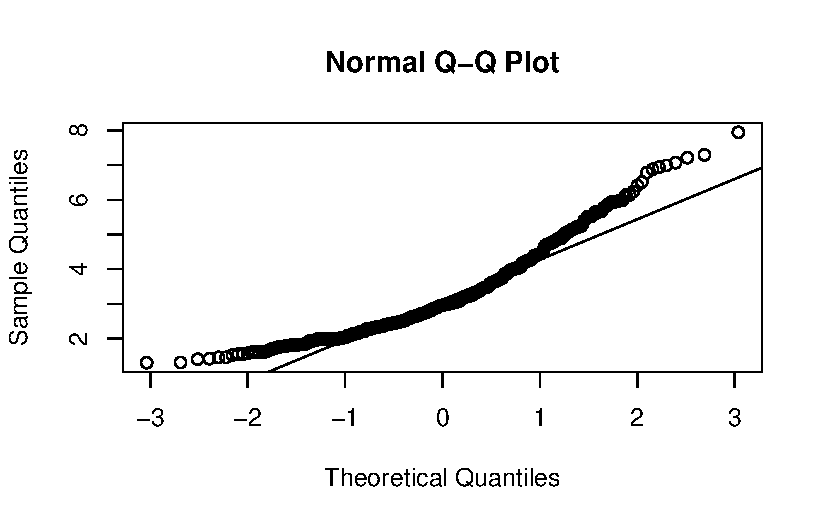
\includegraphics{./traditional-cfa-workflow_files/figure-pdf/unnamed-chunk-5-1.pdf}

}

\end{figure}

\begin{Shaded}
\begin{Highlighting}[]
\CommentTok{\# Plot the multivariate version of the normal probability plot}
\FunctionTok{plot}\NormalTok{(mardia.object)}

\CommentTok{\# Present the outputs we\textquotesingle{}re interested in}
\FunctionTok{tibble}\NormalTok{(}
  \StringTok{"Skew"} \OtherTok{=}\NormalTok{ mardia.object}\SpecialCharTok{$}\NormalTok{skew,}
  \StringTok{"Skew p{-}value"} \OtherTok{=}\NormalTok{ mardia.object}\SpecialCharTok{$}\NormalTok{p.skew,}
  \StringTok{"Kurtosis"} \OtherTok{=}\NormalTok{ mardia.object}\SpecialCharTok{$}\NormalTok{kurtosis,}
  \StringTok{"Kurtosis p{-}value"} \OtherTok{=}\NormalTok{ mardia.object}\SpecialCharTok{$}\NormalTok{p.kurt}
\NormalTok{) }\SpecialCharTok{\%\textgreater{}\%} 
  
\NormalTok{  knitr}\SpecialCharTok{::}\FunctionTok{kable}\NormalTok{()}
\end{Highlighting}
\end{Shaded}

\begin{longtable}[]{@{}rrrr@{}}
\toprule()
Skew & Skew p-value & Kurtosis & Kurtosis p-value \\
\midrule()
\endhead
2359.475 & 0 & 40.52999 & 0 \\
\bottomrule()
\end{longtable}

The plotted points don't seem to fit the straight line super well, which
suggests that the normalness assumption may not hold here. Also, the
hypothesis tests for skew and kurtosis return some mighty low p-values,
suggesting that we've got lots of each of them. So maybe maximum
likelihood estimation isn't such a good idea here?

The authors proceed with it anyway for pedogogical reasons, because they
want to illustrate how the maximum likelihood estimates differ from
estimates arrived at using other methods.

\begin{quote}
``In actual practice, given the lack of multivariate normality that
seems apparent in the previous results, we would likely not use ML and
instead rely on the alternative estimation approach.''
\end{quote}

\hypertarget{model-fitting}{%
\subsection*{Model Fitting}\label{model-fitting}}
\addcontentsline{toc}{subsection}{Model Fitting}

The researchers who collected the data do what good factor analysts do:
they look to the literature to set up some clear and specific candidate
hypotheses, and see the degree to which this new data is compatible with
each of them.

One of the candidate hypotheses is that a person's toxic striving energy
(`achievement goal orientedness'?) is secretly driven by four platonic
unobservable things, namely:

\begin{enumerate}
\def\labelenumi{\arabic{enumi}.}
\item
  Mastery Approach `MAP' (eg. \emph{``I want to learn as much as
  possible'')};
\item
  Mastery Avoidant `MAV' (eg. \emph{``I want to avoid learning less than
  I possibly could''});
\item
  Performance Approach `PAP' (eg. \emph{``I want to do well compared to
  other students'');}
\item
  Performance Avoidant `PAV' (eg. \emph{``It is important for me to
  avoid doing poorly compared to other students''})
\end{enumerate}

We'll call the above hypothesis \textbf{H1.} But there's another
hypothesis that says actually the `Mastery' variables are just one
monolithic thing, so really there are only 3 factors, namely `Mastery',
`PAP', and `PAV'. We'll call this one \textbf{H2.} These will be the two
candidate hypotheses we're gonna test via factor analysis.

The way \textbf{lavaan} works is that you need to separately define the
model syntax as a string, and then feed that string to one of the
model-fitting functions like \texttt{cfa()} . Then we can call the
\texttt{summary()} function to get a big table of outputs.

\begin{Shaded}
\begin{Highlighting}[]
\CommentTok{\# Define the relationships from my hypothesis}
\NormalTok{h1.definition }\OtherTok{\textless{}{-}} 
\StringTok{\textquotesingle{}map=\textasciitilde{}ags1+ags5+ags7}
\StringTok{mav=\textasciitilde{}ags2+ags6+ags12}
\StringTok{pap=\textasciitilde{}ags3+ags9+ags11}
\StringTok{pav=\textasciitilde{}ags4+ags8+ags10\textquotesingle{}}

\CommentTok{\# Fit the model}
\NormalTok{h1.fit }\OtherTok{\textless{}{-}} \FunctionTok{cfa}\NormalTok{(}
  \AttributeTok{data  =}\NormalTok{ dat\_ags,}
  \AttributeTok{model =}\NormalTok{ h1.definition}
\NormalTok{)}

\CommentTok{\# Look at the results}
\NormalTok{h1.summary }\OtherTok{\textless{}{-}} \FunctionTok{summary}\NormalTok{(h1.fit, }\AttributeTok{fit.measures =} \ConstantTok{TRUE}\NormalTok{, }\AttributeTok{standardized =} \ConstantTok{TRUE}\NormalTok{)}

\NormalTok{h1.summary}
\end{Highlighting}
\end{Shaded}

\begin{verbatim}
lavaan 0.6.16 ended normally after 48 iterations

  Estimator                                         ML
  Optimization method                           NLMINB
  Number of model parameters                        30

                                                  Used       Total
  Number of observations                           419         432

Model Test User Model:
                                                      
  Test statistic                               328.312
  Degrees of freedom                                48
  P-value (Chi-square)                           0.000

Model Test Baseline Model:

  Test statistic                              3382.805
  Degrees of freedom                                66
  P-value                                        0.000

User Model versus Baseline Model:

  Comparative Fit Index (CFI)                    0.915
  Tucker-Lewis Index (TLI)                       0.884

Loglikelihood and Information Criteria:

  Loglikelihood user model (H0)              -7014.070
  Loglikelihood unrestricted model (H1)      -6849.914
                                                      
  Akaike (AIC)                               14088.141
  Bayesian (BIC)                             14209.277
  Sample-size adjusted Bayesian (SABIC)      14114.078

Root Mean Square Error of Approximation:

  RMSEA                                          0.118
  90 Percent confidence interval - lower         0.106
  90 Percent confidence interval - upper         0.130
  P-value H_0: RMSEA <= 0.050                    0.000
  P-value H_0: RMSEA >= 0.080                    1.000

Standardized Root Mean Square Residual:

  SRMR                                           0.055

Parameter Estimates:

  Standard errors                             Standard
  Information                                 Expected
  Information saturated (h1) model          Structured

Latent Variables:
                   Estimate  Std.Err  z-value  P(>|z|)   Std.lv  Std.all
  map =~                                                                
    ags1              1.000                               0.840    0.746
    ags5              0.774    0.057   13.564    0.000    0.650    0.682
    ags7              1.100    0.064   17.263    0.000    0.924    0.895
  mav =~                                                                
    ags2              1.000                               0.923    0.627
    ags6              0.974    0.078   12.523    0.000    0.899    0.796
    ags12             1.039    0.096   10.805    0.000    0.959    0.644
  pap =~                                                                
    ags3              1.000                               1.284    0.840
    ags9              0.853    0.038   22.349    0.000    1.095    0.870
    ags11             1.103    0.052   21.178    0.000    1.416    0.841
  pav =~                                                                
    ags4              1.000                               0.929    0.771
    ags8              1.599    0.084   19.091    0.000    1.486    0.855
    ags10             1.525    0.073   20.861    0.000    1.418    0.921

Covariances:
                   Estimate  Std.Err  z-value  P(>|z|)   Std.lv  Std.all
  map ~~                                                                
    mav               0.709    0.079    9.000    0.000    0.914    0.914
    pap               0.066    0.060    1.093    0.274    0.061    0.061
    pav               0.056    0.043    1.289    0.197    0.072    0.072
  mav ~~                                                                
    pap               0.163    0.072    2.265    0.023    0.138    0.138
    pav               0.178    0.053    3.355    0.001    0.207    0.207
  pap ~~                                                                
    pav               1.143    0.102   11.236    0.000    0.958    0.958

Variances:
                   Estimate  Std.Err  z-value  P(>|z|)   Std.lv  Std.all
   .ags1              0.562    0.047   11.951    0.000    0.562    0.443
   .ags5              0.486    0.038   12.780    0.000    0.486    0.535
   .ags7              0.211    0.032    6.602    0.000    0.211    0.198
   .ags2              1.312    0.102   12.825    0.000    1.312    0.606
   .ags6              0.469    0.049    9.537    0.000    0.469    0.367
   .ags12             1.300    0.103   12.669    0.000    1.300    0.586
   .ags3              0.690    0.059   11.671    0.000    0.690    0.295
   .ags9              0.386    0.036   10.769    0.000    0.386    0.244
   .ags11             0.831    0.071   11.639    0.000    0.831    0.293
   .ags4              0.588    0.045   12.959    0.000    0.588    0.405
   .ags8              0.815    0.070   11.602    0.000    0.815    0.269
   .ags10             0.362    0.043    8.423    0.000    0.362    0.153
    map               0.706    0.083    8.514    0.000    1.000    1.000
    mav               0.852    0.128    6.655    0.000    1.000    1.000
    pap               1.648    0.158   10.416    0.000    1.000    1.000
    pav               0.864    0.094    9.198    0.000    1.000    1.000
\end{verbatim}

\begin{Shaded}
\begin{Highlighting}[]
\NormalTok{semPlot}\SpecialCharTok{::}\FunctionTok{semPaths}\NormalTok{(h1.fit)}
\end{Highlighting}
\end{Shaded}

\begin{figure}[H]

{\centering 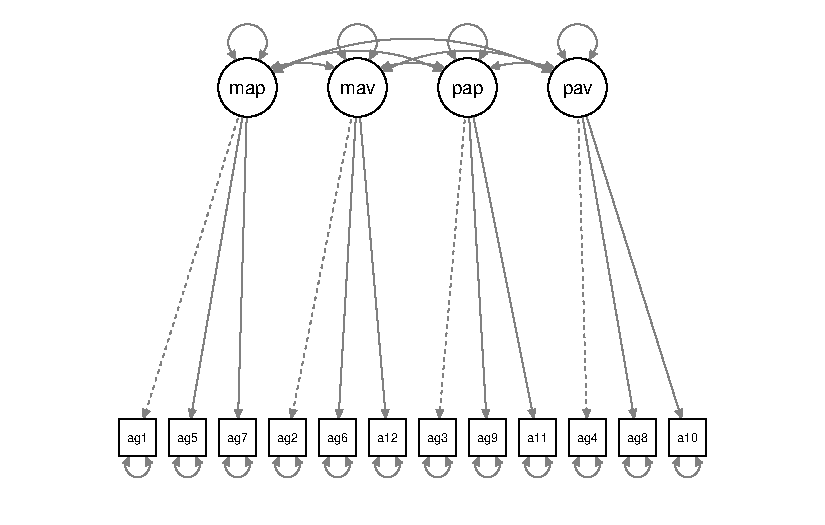
\includegraphics{./traditional-cfa-workflow_files/figure-pdf/unnamed-chunk-6-1.pdf}

}

\end{figure}

That's a lot of outputs. Let's break down the output into smaller
bite-sized chunks.

\hypertarget{goodness-of-fit-statistics}{%
\subsection*{Goodness of Fit
Statistics}\label{goodness-of-fit-statistics}}
\addcontentsline{toc}{subsection}{Goodness of Fit Statistics}

\hypertarget{chi-squared-statistic}{%
\subsubsection*{Chi-Squared Statistic}\label{chi-squared-statistic}}
\addcontentsline{toc}{subsubsection}{Chi-Squared Statistic}

The first thing to look at is the chi-squared statistic from the `User
Model', IE the model I, the user, have just fit. I like to think of this
as a measure of how different the model's reconstructed correlation
matrix looks compared to the actual empirical correlation matrix of the
data. So we use this statistic to test the null hypothesis ``there is no
significant difference between model's reconstructed correlation matrix
and the empirical one''. So, confusingly, we're actually hoping to
\emph{accept} the null hypothesis here. This model returns a value of
328.312 with a vanishingly small p-value, so we reject the null
hypothesis, which is bad: it suggests our model isn't doing a good job
replicating the empirical correlation matrix.

Here's a quote from Gorsuch (1983) that explains this stuff from the
slightly different angle:

\begin{quote}
``The test of significance {[}for a CFA model fit by maximum
likelihood{]} gives a chi-square statistic with the null hypothesis
being that all the population covariance has been extracted by the
hypothesized number of factors. If the chi-square is significant at the
designated probability level, then the residual matrix still has
significant covariance in it.''
\end{quote}

So this chi-squared statistic provides a first look at goodness-of-fit,
but Finch (2015) say it is actually not very trustworthy in practice
because the null hypothesis is sort of crazy: we want a more permissive
test than just whether the model is \emph{perfectly} recreating the
empirical correlation matrix.

\begin{quote}
``this statistic is not particularly useful in practice because it tests
the null hypothesis that {[}the model-reconstructed correlation matrix
is equal to the empirical correlation matrix{]}, which is very
restrictive. The test will almost certainly be rejected when the sample
size is sufficiently large\ldots{} In addition, the chi-square test
relies on the assumption of multivariate normality of the indicators,
which may not be tenable in many situations.''
\end{quote}

So we're gonna wanna look at statistics other than just chi-squared for
goodness-of-fit, but it seems like a fine place to start. Let's look at
the chi-squared statistic of our model:

\begin{Shaded}
\begin{Highlighting}[]
\DocumentationTok{\#\#\# Create a nice summary table}
\FunctionTok{tibble}\NormalTok{(}
  \AttributeTok{Test             =} \StringTok{"standard chi{-}squared"}\NormalTok{,}
  \StringTok{\textasciigrave{}}\AttributeTok{DF}\StringTok{\textasciigrave{}}             \OtherTok{=}\NormalTok{ h1.summary}\SpecialCharTok{$}\NormalTok{test}\SpecialCharTok{$}\NormalTok{standard}\SpecialCharTok{$}\NormalTok{df,}
  \StringTok{\textasciigrave{}}\AttributeTok{Test Statistic}\StringTok{\textasciigrave{}} \OtherTok{=} \FunctionTok{round}\NormalTok{(h1.summary}\SpecialCharTok{$}\NormalTok{test}\SpecialCharTok{$}\NormalTok{standard}\SpecialCharTok{$}\NormalTok{stat, }\DecValTok{2}\NormalTok{),}
  \StringTok{\textasciigrave{}}\AttributeTok{p{-}value}\StringTok{\textasciigrave{}}        \OtherTok{=}\NormalTok{ h1.summary}\SpecialCharTok{$}\NormalTok{test}\SpecialCharTok{$}\NormalTok{standard}\SpecialCharTok{$}\NormalTok{pvalue}
\NormalTok{) }\SpecialCharTok{\%\textgreater{}\%} 
  
  \FunctionTok{mutate}\NormalTok{(}\FunctionTok{across}\NormalTok{(}\FunctionTok{everything}\NormalTok{(), as.character)) }\SpecialCharTok{\%\textgreater{}\%} 
  
  \FunctionTok{pivot\_longer}\NormalTok{(}\FunctionTok{everything}\NormalTok{()) }\SpecialCharTok{\%\textgreater{}\%} 
  
\NormalTok{  knitr}\SpecialCharTok{::}\FunctionTok{kable}\NormalTok{()}
\end{Highlighting}
\end{Shaded}

\begin{longtable}[]{@{}ll@{}}
\toprule()
name & value \\
\midrule()
\endhead
Test & standard chi-squared \\
DF & 48 \\
Test Statistic & 328.31 \\
p-value & 0 \\
\bottomrule()
\end{longtable}

It takes lots of skill and experience to have a sense of whether a test
statistic is big or small given the degrees of freedom at play, but we
can see from the p-value that we reject the null hypothesis in a big
way. This is bad -- it suggests that, given our assumptions, there's a
big difference between our model and the data.

\hypertarget{root-mean-squared-error-approximation-rmsea}{%
\subsubsection*{Root Mean Squared Error Approximation
(RMSEA)}\label{root-mean-squared-error-approximation-rmsea}}
\addcontentsline{toc}{subsubsection}{Root Mean Squared Error
Approximation (RMSEA)}

Another one people like to go with is the Root Mean Squared Error
Approximation (RMSEA). This statistic takes some math and background to
understand, which I'm not going to go over here. I found
\href{http://www.statpower.net/Content/312/Handout/Measures\%20of\%20Fit\%20in\%20Structural\%20Equation\%20Modeling.pdf}{this
document} to be the clearest (but also pretty mathy) explanation.

Essentially, RMSEA is a weighted sum of the discrepancies between the
model's reconstructed correlation matrix and the empirical correlation
matrix. But it also does a nice thing where it discounts model
complexity and sample size to help us not overfit. Here's the
definition:

\(\text{RMSEA} = \sqrt{\dfrac{χ^2 - \text{df}}{\text{df}(n-1)}}\)

See how it takes the chi-squared statistic and divides it by degrees of
freedom (as a proxy for model complexity) and sample size? This makes
for a more conservative measure of goodness-of-fit. Apparently the
square-root is used \emph{``to return the index to the same metric as
the original standardized parameters''}. I don't really understand that
part\ldots{} is it because a Chi-squared random variable is the squared
version of a normal standard variable?

As with the raw chi-squared statistic, we want RMSEA to be small because
it is intended as a measure of the distance between the empirical
correlation matrix and the model-estimated correlation matrix. According
to Finch (2015), people like to say:

\begin{itemize}
\item
  RMSEA \textless= 0.05 is a `good fit';
\item
  0.05 \textless{} RMSEA \textless= 0.08 is an `ok fit'
\item
  RMSEA \textgreater{} .08 is a `bad fit'.
\end{itemize}

Let's check the RMSEA of our model:

\begin{Shaded}
\begin{Highlighting}[]
\CommentTok{\# make a nice summary table}
\NormalTok{h1.summary}\SpecialCharTok{$}\NormalTok{fit }\SpecialCharTok{\%\textgreater{}\%} 
  
  \FunctionTok{as\_tibble}\NormalTok{(}\AttributeTok{rownames =} \StringTok{"stat"}\NormalTok{) }\SpecialCharTok{\%\textgreater{}\%} 
  
  \FunctionTok{filter}\NormalTok{(}\FunctionTok{str\_detect}\NormalTok{(stat, }\StringTok{"rmsea"}\NormalTok{)) }\SpecialCharTok{\%\textgreater{}\%} 
  
\NormalTok{  knitr}\SpecialCharTok{::}\FunctionTok{kable}\NormalTok{()}
\end{Highlighting}
\end{Shaded}

\begin{longtable}[]{@{}lr@{}}
\toprule()
stat & value \\
\midrule()
\endhead
rmsea & 0.1180574 \\
rmsea.ci.lower & 0.1061525 \\
rmsea.ci.upper & 0.1303058 \\
rmsea.ci.level & 0.9000000 \\
rmsea.pvalue & 0.0000000 \\
rmsea.close.h0 & 0.0500000 \\
rmsea.notclose.pvalue & 0.9999999 \\
rmsea.notclose.h0 & 0.0800000 \\
\bottomrule()
\end{longtable}

Yikes -- looks like our whole RMSEA, as well as its confidence interval,
are above the `bad fit' conventional threshold of .08. This corroborates
what we saw with the chi-squared statistic above.

\hypertarget{comparative-fit-index-cfi-and-tucker-lewis-index-tli}{%
\subsubsection*{Comparative Fit Index (CFI) and Tucker-Lewis Index
(TLI)}\label{comparative-fit-index-cfi-and-tucker-lewis-index-tli}}
\addcontentsline{toc}{subsubsection}{Comparative Fit Index (CFI) and
Tucker-Lewis Index (TLI)}

CFI seems to be the most trusted and widely-used tool for assessing
goodness of fit in a CFA. Basically the idea is that we ask: ``how much
does the chi-squared statistic of my model differ from the chi-squared
statistic of the worst model I can think of?'', where the conventional
``worst model I can think of'' is the model where I assume all of my
observed variables are totally uncorrelated. This sort of has the
opposite flavour of the deviance statistic I'm already familiar with,
which compares the current model with ``the best model I can think of.''

\(\text{CFI} = 1 - \dfrac{\text{max}(χ^2_T - \text{df}_T, 0)}{\text{max}(χ^2_0 - \text{df}_0, 0)}\)

Actually, the numerator and denominator are both equal to the
`non-centrality parameter' of their respective candidate distributions.
I'm not gonna get into this, but this is an idea that also shows up in
power analysis as a way of comparing the null and candidate hypotheses.

We want to end up with a CFI as close to 1 as possible, because that
suggests a big difference between my model and the worst possible model.
So people say we can sort of think of this as analogous to \(R^2\) from
linear regression. People seem to have adopted 0.95 as an arbitrary
cutoff for `good fit' for the CFI.

If you want to learn more about the CFI, I found
\href{https://scholarworks.umass.edu/cgi/viewcontent.cgi?article=1561\&context=pare}{this
article} a well-written resource.

Tucker-Lewis Index seems to be pretty similar to CFI, and we interpret
it in the same way. Let's look at both of them:

\begin{Shaded}
\begin{Highlighting}[]
\CommentTok{\# Make a nice summary table}
\NormalTok{h1.summary}\SpecialCharTok{$}\NormalTok{fit }\SpecialCharTok{\%\textgreater{}\%} 
  
  \FunctionTok{as\_tibble}\NormalTok{(}\AttributeTok{rownames =} \StringTok{"stat"}\NormalTok{) }\SpecialCharTok{\%\textgreater{}\%} 
  
  \FunctionTok{filter}\NormalTok{(}\FunctionTok{str\_detect}\NormalTok{(stat, }\StringTok{"cfi|tli"}\NormalTok{)) }\SpecialCharTok{\%\textgreater{}\%} 
  
\NormalTok{  knitr}\SpecialCharTok{::}\FunctionTok{kable}\NormalTok{()}
\end{Highlighting}
\end{Shaded}

\begin{longtable}[]{@{}lr@{}}
\toprule()
stat & value \\
\midrule()
\endhead
cfi & 0.9154874 \\
tli & 0.8837951 \\
\bottomrule()
\end{longtable}

Looks like the CFI and TLI look ok, but don't meet the conventional .95
cutoff. So they are in line with the chi-squared and RMSEA in suggesting
that our goodness-of-fit isn't so good.

\hypertarget{convergent-validty}{%
\subsection*{Convergent Validty}\label{convergent-validty}}
\addcontentsline{toc}{subsection}{Convergent Validty}

Like I said before: when I'm doing factor analysis, my goal is to
convince my research peers that my observed variables are confounded by
an unobserved variable, and that therefore they provide a way of
`measuring' that unobserved variable. This seems like an ontologically
dubious framing, and it also seems impossible to prove. But people who
do research have settled on a few ways of trying to make this case.

One such way is to take all of the measured variables I'm imagining to
be caused by the same unmeasured factor and show that they are indeed
correlated with each other, because this is what we would expect under
the simple DAG where they are all confounded by the same latent
variable. When this happens, I can say that my factor has
\textbf{Convergent Validity.} In the words of Gorsuch (1983):

\begin{quote}
\emph{``Convergent validity occurs when several variables deemed to
measure the same construct correlate with each other.''}
\end{quote}

Or, as Kline (2011) puts it:

\begin{quote}
\emph{``Variables presumed to measure the same construct show convergent
validity if their intercorrelations are appreciable in magnitude.''}
\end{quote}

It seems like to make the jump from `these measured variables are
correlated' to `these measured variables are \emph{caused} by a single
shared latent factor' I would need to be also making the further
assumption that there aren't \emph{other} unmeasured confounders
muddying up the observed covariances. It's DAGs all the way down\ldots{}

Based on the textbooks I'm working from, here are a few questions I can
answer if I want to make the case for Convergent Validity:

\begin{enumerate}
\def\labelenumi{\arabic{enumi}.}
\tightlist
\item
  Are the factor loadings statistically significant?
\item
  Are the standardized factor loadings pretty big (IE pretty close to
  1)?
\item
  Are the standardized within-factor loadings pretty similar to each
  other?
\item
  Do the measurements seem to have good `reliability' as measured by
  something like Chronbach's Alpha, Average Variance Extracted, or
  Composite Reliability?
\item
  Are all of the residual variances less than .50, IE is the model
  explaining at least half the variance of each model?
\end{enumerate}

First we can look at the factor loadings. These are essentially just the
regression coefficients of each factor on each of the outcome variables
for which it was allowed to be a covariate. So we want them to be big
and significant.

\begin{Shaded}
\begin{Highlighting}[]
\DocumentationTok{\#\#\# Make a nice summary table of the factor loadings}
\NormalTok{h1.summary}\SpecialCharTok{$}\NormalTok{pe }\SpecialCharTok{\%\textgreater{}\%} 
  
  \FunctionTok{as\_tibble}\NormalTok{() }\SpecialCharTok{\%\textgreater{}\%} 
  
  \CommentTok{\# Keep only the rows with info on factor loadings}
  \FunctionTok{slice}\NormalTok{(}\DecValTok{1}\SpecialCharTok{:}\DecValTok{12}\NormalTok{) }\SpecialCharTok{\%\textgreater{}\%} 
  
  \CommentTok{\# Clean up the important values, then combine them into a single column}
  \FunctionTok{mutate}\NormalTok{(}
    \AttributeTok{std.all =} \FunctionTok{round}\NormalTok{(std.all, }\DecValTok{2}\NormalTok{),}
    \AttributeTok{std.all =} \FunctionTok{paste0}\NormalTok{(std.all, }\StringTok{", pvalue = "}\NormalTok{, pvalue, }\StringTok{")"}\NormalTok{)}
\NormalTok{  ) }\SpecialCharTok{\%\textgreater{}\%} 
  
  \CommentTok{\# reformat the table}
  \FunctionTok{select}\NormalTok{(lhs, rhs, std.all) }\SpecialCharTok{\%\textgreater{}\%} 
  
  \FunctionTok{pivot\_wider}\NormalTok{(}
    \AttributeTok{names\_from =} \StringTok{"lhs"}\NormalTok{, }
    \AttributeTok{values\_from =} \StringTok{"std.all"}\NormalTok{,}
    \AttributeTok{values\_fill =} \StringTok{"0"}
\NormalTok{  ) }\SpecialCharTok{\%\textgreater{}\%} 
  
  \FunctionTok{column\_to\_rownames}\NormalTok{(}\StringTok{"rhs"}\NormalTok{) }\SpecialCharTok{\%\textgreater{}\%} 
  
\NormalTok{  knitr}\SpecialCharTok{::}\FunctionTok{kable}\NormalTok{(}\AttributeTok{caption =} \StringTok{"Standardized factor loadings and p{-}values"}\NormalTok{)}
\end{Highlighting}
\end{Shaded}

\begin{longtable}[]{@{}
  >{\raggedright\arraybackslash}p{(\columnwidth - 8\tabcolsep) * \real{0.0732}}
  >{\raggedright\arraybackslash}p{(\columnwidth - 8\tabcolsep) * \real{0.2317}}
  >{\raggedright\arraybackslash}p{(\columnwidth - 8\tabcolsep) * \real{0.2317}}
  >{\raggedright\arraybackslash}p{(\columnwidth - 8\tabcolsep) * \real{0.2317}}
  >{\raggedright\arraybackslash}p{(\columnwidth - 8\tabcolsep) * \real{0.2317}}@{}}
\caption{Standardized factor loadings and p-values}\tabularnewline
\toprule()
\begin{minipage}[b]{\linewidth}\raggedright
\end{minipage} & \begin{minipage}[b]{\linewidth}\raggedright
map
\end{minipage} & \begin{minipage}[b]{\linewidth}\raggedright
mav
\end{minipage} & \begin{minipage}[b]{\linewidth}\raggedright
pap
\end{minipage} & \begin{minipage}[b]{\linewidth}\raggedright
pav
\end{minipage} \\
\midrule()
\endfirsthead
\toprule()
\begin{minipage}[b]{\linewidth}\raggedright
\end{minipage} & \begin{minipage}[b]{\linewidth}\raggedright
map
\end{minipage} & \begin{minipage}[b]{\linewidth}\raggedright
mav
\end{minipage} & \begin{minipage}[b]{\linewidth}\raggedright
pap
\end{minipage} & \begin{minipage}[b]{\linewidth}\raggedright
pav
\end{minipage} \\
\midrule()
\endhead
ags1 & 0.75, pvalue = NA) & 0 & 0 & 0 \\
ags5 & 0.68, pvalue = 0) & 0 & 0 & 0 \\
ags7 & 0.9, pvalue = 0) & 0 & 0 & 0 \\
ags2 & 0 & 0.63, pvalue = NA) & 0 & 0 \\
ags6 & 0 & 0.8, pvalue = 0) & 0 & 0 \\
ags12 & 0 & 0.64, pvalue = 0) & 0 & 0 \\
ags3 & 0 & 0 & 0.84, pvalue = NA) & 0 \\
ags9 & 0 & 0 & 0.87, pvalue = 0) & 0 \\
ags11 & 0 & 0 & 0.84, pvalue = 0) & 0 \\
ags4 & 0 & 0 & 0 & 0.77, pvalue = NA) \\
ags8 & 0 & 0 & 0 & 0.85, pvalue = 0) \\
ags10 & 0 & 0 & 0 & 0.92, pvalue = 0) \\
\bottomrule()
\end{longtable}

Firstly, notice that all of the non-fixed loadings are highly
statistically significant, with all p-values smaller than .01. This is
good! Super statistically-significant loadings are a necessary sign that
our measured variables are actually good proxies for the imaginary
`latent' factor we're purporting to use them to measure.

Next, Kline (2011) says that we can start assessing convergent validity
by just looking at the standardized loadings can in isolation. In his
words on page 344:

\begin{quote}
\emph{``{[}with reference to a CFA model he has fit{]}: A few other
standardized coefficients are rather low, such as .433 for the self-talk
indicator of constructive thinking, so evidence for convergent validity
is mixed.''}
\end{quote}

To my eye it looks like some of the standardized loadings on the `mav'
factor are pretty low. Also, it seems like only `pap' has really
consistent loadings across all of its measured variables: the other
three factors all have a bunch of variance between their loadings. So
this all seems like a bit of a red flag.

Kline (2011), on page 307, gives yet another way of assessing convergent
validity: he fits a CFA, then asks whether ``the majority'' of the
variances of the observed variables have been explained, IE whether the
standardized residual variances are \textless50. I guess the idea is
that the amount of variance explained for a variable by a factor depends
on how correlated In his words:

\begin{quote}
``{[}in reference to one of his models:{]} {[}the{]} model fails to
explain the majority (\textgreater{} .50) of variance for a total of
four out of eight indicators, which indicates poor convergent
validity.''
\end{quote}

Let's have a look at the residual variances. These are just the
proportion of the empirical variance of each measured variable that is
left unexplained by the linear models that make up the factor analysis.

\begin{Shaded}
\begin{Highlighting}[]
\NormalTok{h1.summary}\SpecialCharTok{$}\NormalTok{pe }\SpecialCharTok{\%\textgreater{}\%} 
  
  \FunctionTok{as.data.frame}\NormalTok{() }\SpecialCharTok{\%\textgreater{}\%} 
  
  \FunctionTok{filter}\NormalTok{(}\FunctionTok{grepl}\NormalTok{(}\StringTok{"ags}\SpecialCharTok{\textbackslash{}\textbackslash{}}\StringTok{d"}\NormalTok{, lhs)) }\SpecialCharTok{\%\textgreater{}\%} 
  
  \FunctionTok{mutate}\NormalTok{(}\AttributeTok{factor =} \FunctionTok{case\_when}\NormalTok{(}
\NormalTok{    lhs }\SpecialCharTok{\%in\%} \FunctionTok{c}\NormalTok{(}\StringTok{"ags1"}\NormalTok{, }\StringTok{"ags5"}\NormalTok{, }\StringTok{"ags7"}\NormalTok{) }\SpecialCharTok{\textasciitilde{}} \StringTok{"map"}\NormalTok{,}
\NormalTok{    lhs }\SpecialCharTok{\%in\%} \FunctionTok{c}\NormalTok{(}\StringTok{"ags2"}\NormalTok{, }\StringTok{"ags6"}\NormalTok{, }\StringTok{"ags12"}\NormalTok{) }\SpecialCharTok{\textasciitilde{}} \StringTok{"mav"}\NormalTok{,}
\NormalTok{    lhs }\SpecialCharTok{\%in\%} \FunctionTok{c}\NormalTok{(}\StringTok{"ags3"}\NormalTok{, }\StringTok{"ags9"}\NormalTok{, }\StringTok{"ags11"}\NormalTok{) }\SpecialCharTok{\textasciitilde{}} \StringTok{"pap"}\NormalTok{,}
\NormalTok{    lhs }\SpecialCharTok{\%in\%} \FunctionTok{c}\NormalTok{(}\StringTok{"ags4"}\NormalTok{, }\StringTok{"ags8"}\NormalTok{, }\StringTok{"ags10"}\NormalTok{) }\SpecialCharTok{\textasciitilde{}} \StringTok{"pav"}\NormalTok{,}
\NormalTok{  )) }\SpecialCharTok{\%\textgreater{}\%} 
  
  \FunctionTok{select}\NormalTok{(factor, }\StringTok{"var"} \OtherTok{=}\NormalTok{ lhs, std.all) }\SpecialCharTok{\%\textgreater{}\%} 
  
\NormalTok{  knitr}\SpecialCharTok{::}\FunctionTok{kable}\NormalTok{()}
\end{Highlighting}
\end{Shaded}

\begin{longtable}[]{@{}llr@{}}
\toprule()
factor & var & std.all \\
\midrule()
\endhead
map & ags1 & 0.4434896 \\
map & ags5 & 0.5345470 \\
map & ags7 & 0.1980907 \\
mav & ags2 & 0.6063553 \\
mav & ags6 & 0.3670913 \\
mav & ags12 & 0.5858185 \\
pap & ags3 & 0.2950189 \\
pap & ags9 & 0.2436200 \\
pap & ags11 & 0.2927905 \\
pav & ags4 & 0.4050030 \\
pav & ags8 & 0.2694999 \\
pav & ags10 & 0.1526773 \\
\bottomrule()
\end{longtable}

Looks like the model has mostly done a good job for the `Performance'
factors, with all variables having at least \textasciitilde60\% of their
variance explained. But the `Mastery' factors are worse, especially
`mav', with two of its three variables having only \textasciitilde40\%
of their variances explained. This is yet more evidence that the `mav'
factor isn't doing so great a job.

\textasciitilde\textasciitilde Lastly, Gorsuch suggests another way of
testing for convergent validity:

\begin{quote}
\emph{factor loadings of several variables hypothesized to relate to the
construct can also be tested for significance. They could be specified
as equal for the one model and the chi-square for that model subtracted
from another hypothesized factor structure where they are allowed to
vary. If the two differ significantly from each other, then one or more
of the variables is more related to the construct than one or more of
the other variables.''}
\end{quote}

Let's try this out: we'll fit another model that assumes all of the
within-factor loadings are equal, and see if that results in a
statistically significant reduction in goodness-of-fit. If it does, then
we lose some evidence of convergent
validity.\textasciitilde\textasciitilde{}

\hypertarget{reliability}{%
\subsection*{Reliability}\label{reliability}}
\addcontentsline{toc}{subsection}{Reliability}

In looking for Convergent Validity we were mostly just comparing the
parameter estimates (loadings) and residual variances of individual
variables. We were trying to figure out whether these variables belong
together. But in addition to tests of validity to decide which columns
belong in the scale, people like to test the overall scale itself by
invoking the terrible concept named \textbf{`Reliability'}. Reliability
purports to be `true variance in the underlying construct' as a
proportion of `total variance in the scores of a subscale'. This seems
to me like an ontologically dubious concept, but it's what we're working
with.

This all feels pretty similar to Convergent Validity to me. We're just
trying to show that the data are consistent with all of the factor-level
columns being confounded by the same variable.

The all-time classic `reliability' measure is called \textbf{Cronbach's
Alpha.} Cronbach didn't actually invent it, so hello
\href{https://en.wikipedia.org/wiki/Stigler\%27s_law_of_eponymy}{Stigler's
Law}. Here's what it looks like:

\(\alpha = (\dfrac{k}{1-k}) (1 - \dfrac{\sum\sigma_y^2}{\sigma_T^2})\)

The term on the right is doing most of the work: its denominator is the
variance of the column that contains the rowwise sums of my dataset. Its
numerator is the sum of the variances of each column. So we're asking:
`is the variance of the \emph{sums} larger than the variance of the
individual columns?' This will be true if the columns are generally
pretty correlated, because the sums will \emph{stack up} the raw values,
instead of them cancelling each other out. So really we're just asking:
are the columns generally pretty correlated?`. If my columns are pretty
correlated and I make the standard assumption that \emph{no other latent
factors are influencing my observed values} (an insane assumption), then
I can feel comfortable saying that Cronbach's Alpha is useful for
figuring out whether my measurements are all loading on the same
'latent' variable. Since the observed values are gonna be consistent
with each other if this is true, people like to say that Cronbach's
Alpha gives a picture of \textbf{`Internal Consistency Reliability'.}

Like with Convergent Validity, this is all just another way of asking
how correlated my within-factor measured variables are with each other.

Let's calculate Cronbach's Alpha for each of the subscales I've used to
define my supposed factors:

\begin{Shaded}
\begin{Highlighting}[]
\DocumentationTok{\#\#\# Split the dataset into the subscales assumed by my factor model}
\NormalTok{subscales }\OtherTok{\textless{}{-}} \FunctionTok{list}\NormalTok{(}
  \AttributeTok{map =}\NormalTok{ dat\_ags }\SpecialCharTok{\%\textgreater{}\%} \FunctionTok{select}\NormalTok{(ags1, ags5, ags7),}
  \AttributeTok{mav =}\NormalTok{ dat\_ags }\SpecialCharTok{\%\textgreater{}\%} \FunctionTok{select}\NormalTok{(ags2, ags6, ags12),}
  \AttributeTok{pap =}\NormalTok{ dat\_ags }\SpecialCharTok{\%\textgreater{}\%} \FunctionTok{select}\NormalTok{(ags3, ags9, ags11),}
  \AttributeTok{pav =}\NormalTok{ dat\_ags }\SpecialCharTok{\%\textgreater{}\%} \FunctionTok{select}\NormalTok{(ags4, ags8, ags10)}
\NormalTok{)}

\DocumentationTok{\#\#\# Calculate Chronbach\textquotesingle{}s Alpha for each subscale, then analyze.}
\NormalTok{alphas }\OtherTok{\textless{}{-}}\NormalTok{ subscales }\SpecialCharTok{\%\textgreater{}\%} 
  
  \FunctionTok{map}\NormalTok{(psych}\SpecialCharTok{::}\NormalTok{alpha) }\SpecialCharTok{\%\textgreater{}\%} 
  
  \FunctionTok{map}\NormalTok{(summary) }\SpecialCharTok{\%\textgreater{}\%} 
  
\NormalTok{  knitr}\SpecialCharTok{::}\FunctionTok{kable}\NormalTok{() }
\end{Highlighting}
\end{Shaded}

\begin{verbatim}

Reliability analysis   
 raw_alpha std.alpha G6(smc) average_r S/N   ase mean  sd median_r
      0.82      0.82    0.76       0.6 4.6 0.015  5.9 0.9      0.6

Reliability analysis   
 raw_alpha std.alpha G6(smc) average_r S/N   ase mean  sd median_r
      0.77      0.77    0.71      0.52 3.3 0.018  5.3 1.2     0.45

Reliability analysis   
 raw_alpha std.alpha G6(smc) average_r S/N    ase mean  sd median_r
      0.88      0.89    0.84      0.73 7.9 0.0095  5.4 1.3     0.74

Reliability analysis   
 raw_alpha std.alpha G6(smc) average_r S/N  ase mean  sd median_r
      0.87      0.88    0.85       0.7 7.1 0.01  5.6 1.3     0.72
\end{verbatim}

According to Kline (2011), these all look like good results, so they
help me feel good about claiming convergent validity:

\begin{quote}
``Generally, coefficients around .90 are considered''excellent,'' values
around .80 as ``very good,'' and values about .70 as ``adequate.''''
\end{quote}

Cronbach's Alpha has some drawbacks as a measure of `reliability', which
seem pretty clear to me. For example, as (\textbf{Brown?}) explains:

\begin{itemize}
\item
  What if some of the items in my subscale are confounded by something
  other than our latent factor? That could make things crazy, IE it
  could overstate or understate the `true' Cronbach Alpha.
\item
  Even if there's no other confounding at all, my Cronbach Alpha is
  going to be understated if my variables are all influenced by the
  factor to different degrees, IE if the loadings are different, IE if
  the variables are not `Tau-Equivalent'. And this will almost always be
  the case''

  \begin{quote}
  \emph{``The condition of tau equivalence is frequently not realized in
  actual data sets, in part because the units of measurement are often
  arbitrary.''}
  \end{quote}
\end{itemize}

so Kline (2011) says to also calculate the \textbf{Average Variance
Extracted (AVE)}, which is simply the average of the within-factor
squared factor loadings. This is based on the idea that a squared factor
loading is the variance explained of the variable by that factor. The
convention is that if the AVE \textgreater{} 0.5, then you can feel good
about claiming convergent validity. I guess this makes sense -- seems
like a pretty simple and ad-hoc way of asking whether your loadings are
generally on the same page. But obviously if I have lots of observed
variables defining the factor then I'm at risk of having a bunch of high
loadings and a bunch of low loadings, resulting in a misleadingly
moderate average? To me it seems like we might as well just look at the
raw loadings themselves -- no need to look at an average here.

But just for fun, let's calculate the AVE. Rather than doing it
manually, we can use a ready-made function from the \textbf{semTools}
package

\begin{Shaded}
\begin{Highlighting}[]
\NormalTok{semTools}\SpecialCharTok{::}\FunctionTok{AVE}\NormalTok{(h1.fit) }\SpecialCharTok{\%\textgreater{}\%} 
  
\NormalTok{  knitr}\SpecialCharTok{::}\FunctionTok{kable}\NormalTok{()}
\end{Highlighting}
\end{Shaded}

\begin{longtable}[]{@{}lr@{}}
\toprule()
& x \\
\midrule()
\endhead
map & 0.6115914 \\
mav & 0.4556936 \\
pap & 0.7179750 \\
pav & 0.7422385 \\
\bottomrule()
\end{longtable}

Based on the rule-of-thumb that we want the AVE to be at least .50, it
seems like the `mav' factor is having some trouble. It also had the
lowest Cronbach Alpha. So maybe the observed variables I'm using to
measure it aren't actually doing a great job? This hurts convergent
validity for that factor.

Lastly, we can also try to measure this unicorn of `reliability' by just
directly asking ``what proportion of the total variance is explained by
the factor model?''. People like to do this by summing all the factor
loadings, squaring that sum, and dividing it by itself plus the sum of
the residual variances of the variables (IE dividing it by the total
empirical variance of the variable). They call this one the
\textbf{Composite Reliability (CR).} It is the one that Brown (2006)
says to use.

\begin{Shaded}
\begin{Highlighting}[]
\NormalTok{semTools}\SpecialCharTok{::}\FunctionTok{compRelSEM}\NormalTok{(h1.fit) }\SpecialCharTok{\%\textgreater{}\%} 
  
\NormalTok{  knitr}\SpecialCharTok{::}\FunctionTok{kable}\NormalTok{()}
\end{Highlighting}
\end{Shaded}

\begin{longtable}[]{@{}lr@{}}
\toprule()
& x \\
\midrule()
\endhead
map & 0.8164263 \\
mav & 0.6689921 \\
pap & 0.8803380 \\
pav & 0.9016062 \\
\bottomrule()
\end{longtable}

Apparently the rule of thumb for this one is the same as for Cronbach's
Alpha. So we can feel good about all of them except for `mav', which has
taken a beating via these 3 checks.

\hypertarget{discriminant-validity}{%
\subsection*{Discriminant Validity}\label{discriminant-validity}}
\addcontentsline{toc}{subsection}{Discriminant Validity}

Next let's look at the estimated correlations between the factors. If my
hypothesis H1 is true then we should expect all of the factors to be
pretty uncorrelated from each other, but if H2 is true then we should
expect MAP and MAV to be super correlated with each other, because H2
thinks there's no such thing as MAP and MAV -- there's just one big
`Mastery' factor:

\begin{Shaded}
\begin{Highlighting}[]
\DocumentationTok{\#\#\# Make a nicer version of the correlation matrix of the factors}
  
\NormalTok{h1.summary}\SpecialCharTok{$}\NormalTok{pe }\SpecialCharTok{\%\textgreater{}\%} 
  
  \FunctionTok{as\_tibble}\NormalTok{() }\SpecialCharTok{\%\textgreater{}\%} 
 
  \CommentTok{\# Keep only the rows with info on factor loadings}
  \FunctionTok{slice}\NormalTok{(}\DecValTok{25}\SpecialCharTok{:}\DecValTok{34}\NormalTok{) }\SpecialCharTok{\%\textgreater{}\%} 
 
  \FunctionTok{select}\NormalTok{(lhs, rhs, std.lv) }\SpecialCharTok{\%\textgreater{}\%} 
  
  \FunctionTok{mutate}\NormalTok{(}
    \AttributeTok{std.lv =} \FunctionTok{round}\NormalTok{(std.lv, }\DecValTok{2}\NormalTok{),}
    \FunctionTok{across}\NormalTok{(}\FunctionTok{everything}\NormalTok{(), as.character)}
\NormalTok{  ) }\SpecialCharTok{\%\textgreater{}\%} 
  
  \FunctionTok{pivot\_wider}\NormalTok{(}
    \AttributeTok{names\_from =} \StringTok{"lhs"}\NormalTok{, }
    \AttributeTok{values\_from =} \StringTok{"std.lv"}\NormalTok{,}
    \AttributeTok{values\_fill =} \StringTok{" "} 
\NormalTok{  ) }\SpecialCharTok{\%\textgreater{}\%} 
  
  \FunctionTok{column\_to\_rownames}\NormalTok{(}\StringTok{"rhs"}\NormalTok{) }\SpecialCharTok{\%\textgreater{}\%} 
  
\NormalTok{  knitr}\SpecialCharTok{::}\FunctionTok{kable}\NormalTok{(}\AttributeTok{caption =} \StringTok{"Correlation matrix of the factors"}\NormalTok{)}
\end{Highlighting}
\end{Shaded}

\begin{longtable}[]{@{}lllll@{}}
\caption{Correlation matrix of the factors}\tabularnewline
\toprule()
& map & mav & pap & pav \\
\midrule()
\endfirsthead
\toprule()
& map & mav & pap & pav \\
\midrule()
\endhead
map & 1 & & & \\
mav & 0.91 & 1 & & \\
pap & 0.06 & 0.14 & 1 & \\
pav & 0.07 & 0.21 & 0.96 & 1 \\
\bottomrule()
\end{longtable}

Interesting -- the `Mastery' factors and the `Performance' factors each
seem to be very correlated with each other, while being nice and
uncorrelated with the two factors that make up the other. This suggests
that we have bad \textbf{discriminant validity} between the imagined two
types of `Mastery' and two types of `Performance' -- the model can't
really tell them apart as separate things. This makes it harder for me
to argue that they \emph{are} in fact separate things. But then again,
maybe my hypothesis is that the within-skill factors \emph{should} be
highly correlated. Anyhow, the fact that the `Mastery' and `Performance'
factors are all pretty uncorrelated with each other is a good thing for
both hypotheses.

Brown (2006) gives some nice advice about how to assess discriminant
validty, and how to deal with it if you have it:

\begin{quote}
``In applied research, a factor correlation that exceeds .80 or .85 is
often used as the criterion to define poor discriminant validity. When
two factors are highly overlapping, a common research strategy is to
respecify the model by collapsing the dimensions into a single factor
and determine whether this modification results in a significant
degradation in model fit. If the respecified model provides an
acceptable fit to the data, it is usually favored because of its
superior parsimony.''

Gorsuch (1983) suggests doing something similar:
\end{quote}

\begin{quote}
\emph{``{[}fit the model{]} with the qualification that the correlations
between one or more of the constructs being tested for discriminant
validity is one. The difference between chi-squares from {[}this model
vs the model where the correlations are allowed to freely vary{]} tests
whether the constructs have a correlation significantly less than 1.0.
If the correlation between the factors for the two constructs is not
significantly different from 1.0, the difference chi-square will be
insignificant. This means the null hypothesis of no discriminatory
validity would be accepted. If the difference chi-square is significant,
then the null hypothesis is rejected and the model that assumes
discriminatory validity by allowing the correlation to be less than one
is the more appropriate one.''}
\end{quote}

This has the flavour of a likelihood-ratio test. Let's do it. First we
need to fit the model where the correlation between the Mastery factors
and the correlation between the `Performance' factors are both
constrained to be 1:

\begin{Shaded}
\begin{Highlighting}[]
\CommentTok{\# Define the relationships from my hypothesis}
\NormalTok{h1\_orthogonal.definition }\OtherTok{\textless{}{-}} 
\StringTok{\textquotesingle{}map=\textasciitilde{}ags1+ags5+ags7}
\StringTok{mav=\textasciitilde{}ags2+ags6+ags12}
\StringTok{pap=\textasciitilde{}ags3+ags9+ags11}
\StringTok{pav=\textasciitilde{}ags4+ags8+ags10}

\StringTok{map \textasciitilde{}\textasciitilde{} 1*mav}
\StringTok{pap \textasciitilde{}\textasciitilde{} 1*pav}
\StringTok{\textquotesingle{}}

\CommentTok{\# Fit the model}
\NormalTok{h1\_orthogonal.fit }\OtherTok{\textless{}{-}} \FunctionTok{cfa}\NormalTok{(}
  \AttributeTok{data  =}\NormalTok{ dat\_ags,}
  \AttributeTok{model =}\NormalTok{ h1\_orthogonal.definition}
\NormalTok{)}

\CommentTok{\# Compare the goodness{-}of{-}fit statistics for the two models}
\FunctionTok{anova}\NormalTok{(h1.fit, h1\_orthogonal.fit) }\SpecialCharTok{\%\textgreater{}\%} 
  
\NormalTok{  knitr}\SpecialCharTok{::}\FunctionTok{kable}\NormalTok{()}
\end{Highlighting}
\end{Shaded}

\begin{longtable}[]{@{}
  >{\raggedright\arraybackslash}p{(\columnwidth - 16\tabcolsep) * \real{0.2045}}
  >{\raggedleft\arraybackslash}p{(\columnwidth - 16\tabcolsep) * \real{0.0341}}
  >{\raggedleft\arraybackslash}p{(\columnwidth - 16\tabcolsep) * \real{0.1023}}
  >{\raggedleft\arraybackslash}p{(\columnwidth - 16\tabcolsep) * \real{0.1023}}
  >{\raggedleft\arraybackslash}p{(\columnwidth - 16\tabcolsep) * \real{0.1023}}
  >{\raggedleft\arraybackslash}p{(\columnwidth - 16\tabcolsep) * \real{0.1250}}
  >{\raggedleft\arraybackslash}p{(\columnwidth - 16\tabcolsep) * \real{0.1136}}
  >{\raggedleft\arraybackslash}p{(\columnwidth - 16\tabcolsep) * \real{0.0909}}
  >{\raggedleft\arraybackslash}p{(\columnwidth - 16\tabcolsep) * \real{0.1250}}@{}}
\toprule()
\begin{minipage}[b]{\linewidth}\raggedright
\end{minipage} & \begin{minipage}[b]{\linewidth}\raggedleft
Df
\end{minipage} & \begin{minipage}[b]{\linewidth}\raggedleft
AIC
\end{minipage} & \begin{minipage}[b]{\linewidth}\raggedleft
BIC
\end{minipage} & \begin{minipage}[b]{\linewidth}\raggedleft
Chisq
\end{minipage} & \begin{minipage}[b]{\linewidth}\raggedleft
Chisq diff
\end{minipage} & \begin{minipage}[b]{\linewidth}\raggedleft
RMSEA
\end{minipage} & \begin{minipage}[b]{\linewidth}\raggedleft
Df diff
\end{minipage} & \begin{minipage}[b]{\linewidth}\raggedleft
Pr(\textgreater Chisq)
\end{minipage} \\
\midrule()
\endhead
h1.fit & 48 & 14088.14 & 14209.28 & 328.3120 & NA & NA & NA & NA \\
h1\_orthogonal.fit & 50 & 14096.44 & 14209.50 & 340.6065 & 12.29456 &
0.1108363 & 2 & 0.0021393 \\
\bottomrule()
\end{longtable}

Looks like the reduction in chi-squared goodness-of-fit is statistically
significant when we force the within-skill factors to be perfectly
correlated. So, according to the Gorsuch (1983) quote above, we can
reject the null hypothesis that the within-skill factors are perfectly
correlated. This gives a justification for continuing to distinguish
between them as separate factors, and helps me make a believable claim
that my posited factors are in fact different things.

Actually, I think another way we could have done this would be to just
fit the model where we just define one big factor for `Mastery' and one
big factor for `Performance'. I tried this and it returned even worse
fit, which means the extra parameters (the correlation parameters) are
significantly improving fit in the pure h1 model.

\hypertarget{conclusion}{%
\subsection*{Conclusion}\label{conclusion}}
\addcontentsline{toc}{subsection}{Conclusion}

All-in-all it seems like neither of these hypotheses do a great job.
Sure, the `Performance' factors have good convergent validity, and we
see good discriminant validity between the `Performance' and `Mastery'
factors, but the `Mastery' factors don't have great convergent validity
and fitting a single monolithic `Mastery' factor doesn't improve things.

I can make a better model by dropping the measured `Mastery' variables
that aren't having lots of their variance explained by the `Mastery'
factors, but this is contrary to the spirit of CFA. If I want to test a
different hypothesis then I should collect a different sample.

For a nice template of a more formal presentation of the results of a
CFA, see Brown (2006) chapter 4 appendix 3.

\hypertarget{modification-indexes}{%
\chapter{Modification Indexes}\label{modification-indexes}}

In this chapter we'll work through another example of the Traditional
CFA Workflow to get more practice. We'll also introduce the concept of
`Modification Indexes', which researchers often use to improve their
model goodness of fit in a way that seems a bit suss to me. Probably a
good thing to know about.

\begin{Shaded}
\begin{Highlighting}[]
\FunctionTok{library}\NormalTok{(tidyverse)}
\FunctionTok{library}\NormalTok{(lavaan)}
\FunctionTok{library}\NormalTok{(ggdag)}
\end{Highlighting}
\end{Shaded}

\hypertarget{example-2-biodiversity}{%
\section*{Example 2: Biodiversity}\label{example-2-biodiversity}}
\addcontentsline{toc}{section}{Example 2: Biodiversity}

Here's
\href{https://d9-wret.s3.us-west-2.amazonaws.com/assets/palladium/production/s3fs-public/atoms/files/SEM_09_2-Ex1_CFA_exercise.pdf}{a
fun example from the Wetland and Aquatic Research Center of the U.S.
Geological Survey}: given counts of different types of animals, can we
fit a convincing CFA model for `diversity'? In other words: is the
correlation structure of all my counts of various types of animals
consistent with the possibility that those counts are confounded by a
single unobserved thing called `diversity'?

\begin{Shaded}
\begin{Highlighting}[]
\NormalTok{dat\_raw }\OtherTok{\textless{}{-}} \FunctionTok{read.csv}\NormalTok{(}\StringTok{\textquotesingle{}../data/grace/SEM\_09\_2{-}Ex1\_CFA\_exercise\_data.csv\textquotesingle{}}\NormalTok{)}

\NormalTok{dat\_clean }\OtherTok{\textless{}{-}}\NormalTok{ dat\_raw }\SpecialCharTok{\%\textgreater{}\%}  
  
\NormalTok{  janitor}\SpecialCharTok{::}\FunctionTok{clean\_names}\NormalTok{()}
\end{Highlighting}
\end{Shaded}

\hypertarget{data-exploration-1}{%
\subsection*{Data Exploration}\label{data-exploration-1}}
\addcontentsline{toc}{subsection}{Data Exploration}

Just for fun let's see if the relative proportions of the different
animals varies between countries:

\begin{Shaded}
\begin{Highlighting}[]
\DocumentationTok{\#\#\# Proportions}
\NormalTok{dat\_clean }\SpecialCharTok{\%\textgreater{}\%} 
  
  \FunctionTok{pivot\_longer}\NormalTok{(}
    \AttributeTok{cols      =} \SpecialCharTok{!}\FunctionTok{matches}\NormalTok{(}\StringTok{"\^{}c"}\NormalTok{),}
    \AttributeTok{names\_to  =} \StringTok{"animal"}\NormalTok{,}
    \AttributeTok{values\_to =} \StringTok{"count"}
\NormalTok{  ) }\SpecialCharTok{\%\textgreater{}\%} 
  
  \FunctionTok{group\_by}\NormalTok{(country) }\SpecialCharTok{\%\textgreater{}\%} 
  \FunctionTok{mutate}\NormalTok{(}
    \AttributeTok{total =} \FunctionTok{sum}\NormalTok{(count), }
    \AttributeTok{prop  =} \FunctionTok{round}\NormalTok{(count }\SpecialCharTok{/}\NormalTok{ total, }\DecValTok{2}\NormalTok{)}
\NormalTok{  ) }\SpecialCharTok{\%\textgreater{}\%} 
  \FunctionTok{ungroup}\NormalTok{() }\SpecialCharTok{\%\textgreater{}\%} 

  \FunctionTok{ggplot}\NormalTok{() }\SpecialCharTok{+} 
  \FunctionTok{geom\_bar}\NormalTok{(}\FunctionTok{aes}\NormalTok{(}\AttributeTok{x =}\NormalTok{ animal, }\AttributeTok{y =}\NormalTok{ prop), }\AttributeTok{stat =} \StringTok{"identity"}\NormalTok{) }\SpecialCharTok{+} 
  \FunctionTok{theme\_bw}\NormalTok{() }\SpecialCharTok{+} 
  \FunctionTok{theme}\NormalTok{(}\AttributeTok{axis.text.x =} \FunctionTok{element\_text}\NormalTok{(}\AttributeTok{angle =} \DecValTok{90}\NormalTok{, }\AttributeTok{vjust =} \FloatTok{0.5}\NormalTok{, }\AttributeTok{hjust=}\DecValTok{1}\NormalTok{)) }\SpecialCharTok{+}
  \FunctionTok{facet\_wrap}\NormalTok{(}\SpecialCharTok{\textasciitilde{}}\NormalTok{country)}
\end{Highlighting}
\end{Shaded}

\begin{figure}[H]

{\centering 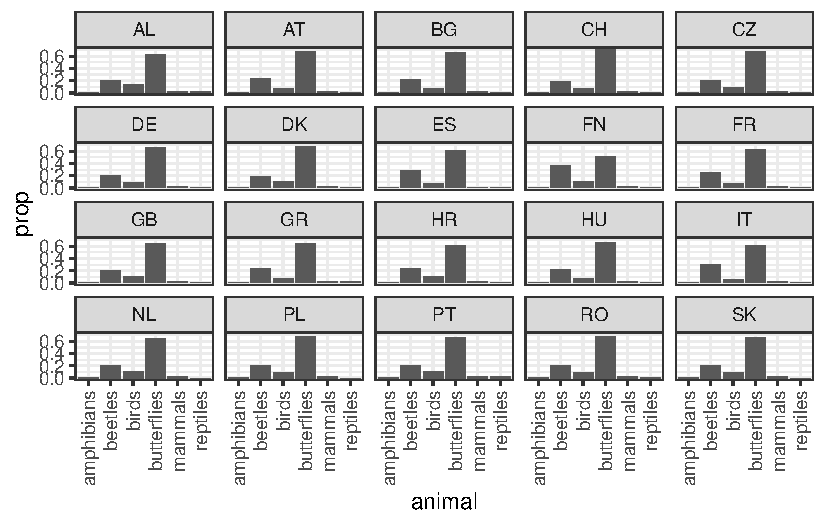
\includegraphics{./modification-indexes_files/figure-pdf/unnamed-chunk-3-1.pdf}

}

\end{figure}

The proportions are pretty stable. Finland seems like the weirdest one,
and it isn't even that weird.

\hypertarget{model-fitting-1}{%
\subsection*{Model Fitting}\label{model-fitting-1}}
\addcontentsline{toc}{subsection}{Model Fitting}

The hypothesis we want to test here is simply that all of these counts
are confounded by a single unmeasured `biodiversity' variable. This is
straightforward to fit:

\begin{Shaded}
\begin{Highlighting}[]
\NormalTok{h1.definition }\OtherTok{\textless{}{-}} 
\StringTok{\textquotesingle{}diversity =\textasciitilde{} mammals + birds + amphibians + reptiles + beetles + butterflies\textquotesingle{}}

\NormalTok{h1.fit }\OtherTok{\textless{}{-}} \FunctionTok{cfa}\NormalTok{(}
  \AttributeTok{data  =}\NormalTok{ dat\_clean }\SpecialCharTok{\%\textgreater{}\%} \FunctionTok{select}\NormalTok{(}\SpecialCharTok{{-}}\NormalTok{country) }\SpecialCharTok{\%\textgreater{}\%} \FunctionTok{scale}\NormalTok{(),}
  \AttributeTok{model =}\NormalTok{ h1.definition}
\NormalTok{)}

\NormalTok{h1.summary }\OtherTok{\textless{}{-}} \FunctionTok{summary}\NormalTok{(h1.fit)}

\NormalTok{h1.summary}
\end{Highlighting}
\end{Shaded}

\begin{verbatim}
lavaan 0.6.16 ended normally after 23 iterations

  Estimator                                         ML
  Optimization method                           NLMINB
  Number of model parameters                        12

  Number of observations                            20

Model Test User Model:
                                                      
  Test statistic                                20.817
  Degrees of freedom                                 9
  P-value (Chi-square)                           0.013

Parameter Estimates:

  Standard errors                             Standard
  Information                                 Expected
  Information saturated (h1) model          Structured

Latent Variables:
                   Estimate  Std.Err  z-value  P(>|z|)
  diversity =~                                        
    mammals           1.000                           
    birds             0.825    0.277    2.978    0.003
    amphibians        1.115    0.260    4.281    0.000
    reptiles          0.780    0.279    2.793    0.005
    beetles           1.135    0.259    4.380    0.000
    butterflies       1.261    0.254    4.960    0.000

Variances:
                   Estimate  Std.Err  z-value  P(>|z|)
   .mammals           0.387    0.131    2.958    0.003
   .birds             0.566    0.184    3.073    0.002
   .amphibians        0.250    0.092    2.727    0.006
   .reptiles          0.608    0.197    3.089    0.002
   .beetles           0.224    0.085    2.645    0.008
   .butterflies       0.054    0.054    1.010    0.313
    diversity         0.563    0.278    2.025    0.043
\end{verbatim}

Let's have a look at the same 4 goodness-of-fit measures we used in the
previous example. We can bring them all together with a nice utility
function:

\begin{Shaded}
\begin{Highlighting}[]
\DocumentationTok{\#\#\# Define a custom function}
\NormalTok{fit\_measures }\OtherTok{\textless{}{-}} \ControlFlowTok{function}\NormalTok{(fit)\{}
  
\NormalTok{  summary }\OtherTok{\textless{}{-}} \FunctionTok{summary}\NormalTok{(fit, }\AttributeTok{fit.measures =} \ConstantTok{TRUE}\NormalTok{, }\AttributeTok{standardized =} \ConstantTok{TRUE}\NormalTok{)}
  
\NormalTok{  res }\OtherTok{\textless{}{-}} \FunctionTok{list}\NormalTok{(}
    
    \CommentTok{\# Chi{-}Squared}
    \AttributeTok{chi\_squared =} \FunctionTok{tibble}\NormalTok{(}
      \AttributeTok{Test             =} \StringTok{"standard chi{-}squared"}\NormalTok{,}
      \StringTok{\textasciigrave{}}\AttributeTok{DF}\StringTok{\textasciigrave{}}             \OtherTok{=}\NormalTok{ summary}\SpecialCharTok{$}\NormalTok{test}\SpecialCharTok{$}\NormalTok{standard}\SpecialCharTok{$}\NormalTok{df,}
      \StringTok{\textasciigrave{}}\AttributeTok{Test Statistic}\StringTok{\textasciigrave{}} \OtherTok{=} \FunctionTok{round}\NormalTok{(summary}\SpecialCharTok{$}\NormalTok{test}\SpecialCharTok{$}\NormalTok{standard}\SpecialCharTok{$}\NormalTok{stat, }\DecValTok{2}\NormalTok{),}
      \StringTok{\textasciigrave{}}\AttributeTok{p{-}value}\StringTok{\textasciigrave{}}        \OtherTok{=}\NormalTok{ summary}\SpecialCharTok{$}\NormalTok{test}\SpecialCharTok{$}\NormalTok{standard}\SpecialCharTok{$}\NormalTok{pvalue) }\SpecialCharTok{\%\textgreater{}\%} 
      
      \FunctionTok{mutate}\NormalTok{(}\FunctionTok{across}\NormalTok{(}\FunctionTok{everything}\NormalTok{(), as.character)) }\SpecialCharTok{\%\textgreater{}\%} 
      
      \FunctionTok{pivot\_longer}\NormalTok{(}\FunctionTok{everything}\NormalTok{()),}
    
    \CommentTok{\# RMSEA}
    \AttributeTok{rmsea =}\NormalTok{ summary}\SpecialCharTok{$}\NormalTok{fit }\SpecialCharTok{\%\textgreater{}\%} 
      
      \FunctionTok{as\_tibble}\NormalTok{(}\AttributeTok{rownames =} \StringTok{"stat"}\NormalTok{) }\SpecialCharTok{\%\textgreater{}\%} 
      
      \FunctionTok{filter}\NormalTok{(}\FunctionTok{str\_detect}\NormalTok{(stat, }\StringTok{"rmsea"}\NormalTok{)),}
    
    \CommentTok{\# CFI and TLI}
    \AttributeTok{cfi\_tli =}\NormalTok{ summary}\SpecialCharTok{$}\NormalTok{fit }\SpecialCharTok{\%\textgreater{}\%} 
      
      \FunctionTok{as\_tibble}\NormalTok{(}\AttributeTok{rownames =} \StringTok{"stat"}\NormalTok{) }\SpecialCharTok{\%\textgreater{}\%} 
      
      \FunctionTok{filter}\NormalTok{(}\FunctionTok{str\_detect}\NormalTok{(stat, }\StringTok{"cfi|tli"}\NormalTok{)) }
    
\NormalTok{  )}
  
\NormalTok{  res}
  
\NormalTok{\}}

\DocumentationTok{\#\#\# Call the function, then send its outputs to clean tables}
\FunctionTok{fit\_measures}\NormalTok{(h1.fit) }\SpecialCharTok{\%\textgreater{}\%} 
  
  \FunctionTok{map}\NormalTok{(knitr}\SpecialCharTok{::}\NormalTok{kable)}
\end{Highlighting}
\end{Shaded}

\begin{verbatim}
$chi_squared


|name           |value                |
|:--------------|:--------------------|
|Test           |standard chi-squared |
|DF             |9                    |
|Test Statistic |20.82                |
|p-value        |0.0134888288206897   |

$rmsea


|stat                  |      value|
|:---------------------|----------:|
|rmsea                 | 0.25622117|
|rmsea.ci.lower        | 0.11034617|
|rmsea.ci.upper        | 0.40224444|
|rmsea.ci.level        | 0.90000000|
|rmsea.pvalue          | 0.01890337|
|rmsea.close.h0        | 0.05000000|
|rmsea.notclose.pvalue | 0.97055608|
|rmsea.notclose.h0     | 0.08000000|

$cfi_tli


|stat |     value|
|:----|---------:|
|cfi  | 0.8695573|
|tli  | 0.7825955|
\end{verbatim}

The model isn't fitting very well -- Chi-Squared is highly statistically
significant (we fail to reject the null hypothesis that there is
residual variance left to explain), RMSEA is well above its conventional
threshold, and CFI and TLI are both well below their conventional
thresholds.

\hypertarget{modification-indexes-1}{%
\subsection*{Modification Indexes}\label{modification-indexes-1}}
\addcontentsline{toc}{subsection}{Modification Indexes}

Here (\textbf{Grace?}) introduces a new method for tweaking our CFA
model to improve goodness of fit. The idea is that we can use fancy math
to ask ``if I took a certain fixed parameter from my model definition
and allowed it to be freely estimated, how much would my model's
chi-squared goodness of fit change?'' People like to take this estimated
change in goodness-of-fit and call it a \textbf{modification index.} As
Brown (2006) puts it:

\begin{quote}
``The modification index reflects an approximation of how much the
overall model \(χ^2\) would decrease if the fixed or constrained
parameter was freely estimated.''
\end{quote}

Apparently conventional cutoff for a `good' modification index is 3.84.
So to get some ideas on how we might improve our goodness-of-fit, let's
print out the modification indexes for each of the fixed parameters in
the model and see which of them pass that threshold:

\begin{Shaded}
\begin{Highlighting}[]
\CommentTok{\# Get the estimated change in chi{-}squared for each fixed parameter}
\FunctionTok{modindices}\NormalTok{(h1.fit) }\SpecialCharTok{\%\textgreater{}\%} 
  
  \CommentTok{\# Arrange them in order of modification index}
  \FunctionTok{arrange}\NormalTok{(}\FunctionTok{desc}\NormalTok{(mi)) }\SpecialCharTok{\%\textgreater{}\%} 
  
  \FunctionTok{select}\NormalTok{(lhs, op, rhs, mi) }\SpecialCharTok{\%\textgreater{}\%} 
  
\NormalTok{  knitr}\SpecialCharTok{::}\FunctionTok{kable}\NormalTok{(}\AttributeTok{digits =} \DecValTok{2}\NormalTok{)}
\end{Highlighting}
\end{Shaded}

\begin{longtable}[]{@{}lllr@{}}
\toprule()
lhs & op & rhs & mi \\
\midrule()
\endhead
birds & \textasciitilde\textasciitilde{} & beetles & 4.44 \\
birds & \textasciitilde\textasciitilde{} & amphibians & 3.99 \\
mammals & \textasciitilde\textasciitilde{} & butterflies & 2.84 \\
beetles & \textasciitilde\textasciitilde{} & butterflies & 2.78 \\
mammals & \textasciitilde\textasciitilde{} & amphibians & 2.31 \\
birds & \textasciitilde\textasciitilde{} & reptiles & 2.05 \\
amphibians & \textasciitilde\textasciitilde{} & butterflies & 1.72 \\
birds & \textasciitilde\textasciitilde{} & butterflies & 1.55 \\
mammals & \textasciitilde\textasciitilde{} & reptiles & 1.29 \\
mammals & \textasciitilde\textasciitilde{} & birds & 1.20 \\
amphibians & \textasciitilde\textasciitilde{} & beetles & 0.58 \\
mammals & \textasciitilde\textasciitilde{} & beetles & 0.38 \\
reptiles & \textasciitilde\textasciitilde{} & butterflies & 0.22 \\
reptiles & \textasciitilde\textasciitilde{} & beetles & 0.15 \\
amphibians & \textasciitilde\textasciitilde{} & reptiles & 0.14 \\
\bottomrule()
\end{longtable}

Based on the operation symbol ``\textasciitilde\textasciitilde{}'', it
seems like all of the modification indexes correspond to residual
correlations between observed variables. This teaches me something about
CFA models! I guess in the typical CFA model we fix the residual
correlations to 0? This helps me understand why the
\href{https://discourse.mc-stan.org/t/confirmatory-factor-analysis-using-brms/23139}{Bayesian
CFA model as implemented in \textbf{brms}} specifies
\texttt{rescor\ =\ FALSE} . I was confused about this!

Actually, I just realized Gorsuch (1983) already explained this to me!
Think back to where he showed us the definition of the `Common Factor
Model':

\(R_{vv} = PR_{ff}P' + U_{vv}\)

And remember how Gorsuch specified that \(U_{vv}\) is assumed to be a
diagonal matrix, IE the residual correlations is assumed to be
uncorrelated for each variable. This is the whole thing about the
`unique factors', IE the error terms, of the linear models of each
measured variable are gonna be uncorrelated.
\href{https://stats.oarc.ucla.edu/r/seminars/rcfa/}{This recorded
seminar and notes from UCLA} give a nice clear walkthrough of the
notation in a slightly different form from Gorsuch (1983).

From the DAGs perspective of CFA, assuming uncorrelated residuals sort
of makes sense to me: if I want to convince you that my measured
variables are all confounded by the same single unmeasured variable,
then I think fixing the residual errors at 0 is a way of committing my
model to the idea that there aren't \emph{other} unmeasured variables
confounding certain of my measured guys. It is a strong assumption that,
if it holds up, provides better evidence that my variables really truly
are just confounded by a single unmeasured thing.

So I guess I could write out this standard CFA model in a more McElreath
fashion like so:

{[} \begin{align*}
\begin{bmatrix} \text{mammals}_i \\ \text{birds}_i \\ \text{amphibians}_i \\ \text{reptiles}_i \\ \text{beetles}_i \\ \end{bmatrix} & \sim
\operatorname{MVNormal} \left( \begin{bmatrix} \mu_{mammals} \\ \mu_{birds} \\ \mu_{amphibians} \\ \mu_{reptiles} \\ \mu_{beetles} \end{bmatrix}, \mathbf{\Sigma} \right)\\
\mu_{mammals} & = \lambda_{mammals} F_i \\
\mu_{birds} & = \lambda_{birds} F_i \\
\mu_{amphibians} & = \lambda_{amphibians} F_i \\
\mu_{reptiles} & = \lambda_{reptiles} F_i \\
\mu_{beetles} & = \lambda_{beetles} F_i \\
\Sigma & = \begin{pmatrix} 
\sigma_{mammals}&0 &0 &0 &0 \\ 
0 & \sigma_{birds} &0 &0 &0 \\ 
0 & 0 & \sigma_{amphibians} &0 &0 \\ 
0 & 0 & 0 & \sigma_{reptiles} &0 \\ 
0 & 0 & 0 & 0 & \sigma_{beetles} 
\end{pmatrix} \\
\end{align*} {]}

In human words: the observed counts of each of the 5 animal types are
imagined to be drawn from a shared multivariate normal distribution. The
mean of each dimension of that distribution is a linear function of a
single shared factor, which we're calling `biodiversity'. The variance
of each dimension of that distribution is unique, and there is no
covariance between the dimensions.

But now think back to our modification indexes: a few of them are saying
that if we allow the residual covariances to be freely estimated rather
than fixed at 0, then we can improve model fit by a whole lot.
Specifically, if we allow the residual covariance between birds and
beetles and/or between birds and amphibians to be freely estimated, then
model fit as measured by the chi-squared statistic might be
significantly improved. Here's what the model is gonna look like now:

{[} \begin{align*}
\begin{bmatrix} \text{mammals}_i \\ \text{birds}_i \\ \text{amphibians}_i \\ \text{reptiles}_i \\ \text{beetles}_i \\ \end{bmatrix} & \sim
\operatorname{MVNormal} \left( \begin{bmatrix} \mu_{mammals} \\ \mu_{birds} \\ \mu_{amphibians} \\ \mu_{reptiles} \\ \mu_{beetles} \end{bmatrix}, \mathbf{\Sigma} \right)\\
\mu_{mammals} & = \lambda_{mammals} F_i \\
\mu_{birds} & = \lambda_{birds} F_i \\
\mu_{amphibians} & = \lambda_{amphibians} F_i \\
\mu_{reptiles} & = \lambda_{reptiles} F_i \\
\mu_{beetles} & = \lambda_{beetles} F_i \\
\Sigma & = \begin{pmatrix} 
\sigma_{mammals}&0 &0 &0 &0 \\ 
0 & \sigma_{birds} &\theta_\text{b\&a} &0 &\theta_\text{b\&b} \\ 
0 &\theta_\text{b\&a} & \sigma_{amphibians} &0 &0 \\ 
0 & 0 & 0 & \sigma_{reptiles} &0 \\ 
0 &\theta_\text{b\&b} & 0 & 0 & \sigma_{beetles} 
\end{pmatrix} \\
\end{align*} {]}

See how I've filled in the variance-covariance matrix of the likelihood
to include a few more free parameters?

Actually, Grace proceeds by fitting two more models, one with each of
these two candidate covariance parameters as freely fitting. Then he
uses \texttt{anova()} to do a likelihood-ratio test for them. We can't
test all 3 models at once because models 2 and 3 aren't nested with each
other.

\begin{Shaded}
\begin{Highlighting}[]
\DocumentationTok{\#\#\# Letting the covariance between birds and beetles be freely estimated}
\NormalTok{h2.definition }\OtherTok{\textless{}{-}} 
\StringTok{\textquotesingle{}diversity =\textasciitilde{} mammals + birds + amphibians + }
\StringTok{              reptiles + beetles + butterflies}
\StringTok{ }
\StringTok{ birds \textasciitilde{}\textasciitilde{} beetles\textquotesingle{}}


\NormalTok{h2.fit }\OtherTok{\textless{}{-}} \FunctionTok{cfa}\NormalTok{(}
  \AttributeTok{data  =}\NormalTok{ dat\_clean }\SpecialCharTok{\%\textgreater{}\%} \FunctionTok{select}\NormalTok{(}\SpecialCharTok{{-}}\NormalTok{country) }\SpecialCharTok{\%\textgreater{}\%} \FunctionTok{scale}\NormalTok{(),}
  \AttributeTok{model =}\NormalTok{ h2.definition}
\NormalTok{)}

\DocumentationTok{\#\#\# Letting the covariance between birds and amphibians be freely estimated}
\NormalTok{h3.definition }\OtherTok{\textless{}{-}} 
  \StringTok{\textquotesingle{}diversity =\textasciitilde{} mammals + birds + amphibians + }
\StringTok{              reptiles + beetles + butterflies}
\StringTok{ }
\StringTok{ birds \textasciitilde{}\textasciitilde{} amphibians\textquotesingle{}}


\NormalTok{h3.fit }\OtherTok{\textless{}{-}} \FunctionTok{cfa}\NormalTok{(}
 \AttributeTok{data  =}\NormalTok{ dat\_clean }\SpecialCharTok{\%\textgreater{}\%} \FunctionTok{select}\NormalTok{(}\SpecialCharTok{{-}}\NormalTok{country) }\SpecialCharTok{\%\textgreater{}\%} \FunctionTok{scale}\NormalTok{(),}
  \AttributeTok{model =}\NormalTok{ h3.definition}
\NormalTok{)}

\FunctionTok{anova}\NormalTok{(h1.fit, h2.fit)}
\end{Highlighting}
\end{Shaded}

\begin{verbatim}

Chi-Squared Difference Test

       Df    AIC    BIC  Chisq Chisq diff   RMSEA Df diff Pr(>Chisq)  
h2.fit  8 270.81 283.76 16.013                                        
h1.fit  9 273.62 285.56 20.817      4.804 0.43612       1    0.02839 *
---
Signif. codes:  0 '***' 0.001 '**' 0.01 '*' 0.05 '.' 0.1 ' ' 1
\end{verbatim}

\begin{Shaded}
\begin{Highlighting}[]
\FunctionTok{anova}\NormalTok{(h1.fit, h3.fit)}
\end{Highlighting}
\end{Shaded}

\begin{verbatim}

Chi-Squared Difference Test

       Df    AIC    BIC  Chisq Chisq diff   RMSEA Df diff Pr(>Chisq)   
h3.fit  8 267.72 280.67 12.924                                         
h1.fit  9 273.62 285.56 20.817     7.8934 0.58709       1   0.004961 **
---
Signif. codes:  0 '***' 0.001 '**' 0.01 '*' 0.05 '.' 0.1 ' ' 1
\end{verbatim}

Looks like model H3 has the lowest AIC and the more significant
improvement in chi-squared fit. So let's continue working with that one
in the following sections.

\hypertarget{validity}{%
\subsection*{Validity}\label{validity}}
\addcontentsline{toc}{subsection}{Validity}

We can do the same 5 checks of validity we used in the previous `Mastery
and Performance' example. Let's start with the big summary printout:

\begin{Shaded}
\begin{Highlighting}[]
\NormalTok{summary.h3 }\OtherTok{\textless{}{-}} \FunctionTok{summary}\NormalTok{(h3.fit, }\AttributeTok{fit.measures =} \ConstantTok{TRUE}\NormalTok{, }\AttributeTok{standardized =} \ConstantTok{TRUE}\NormalTok{)}

\NormalTok{summary.h3}
\end{Highlighting}
\end{Shaded}

\begin{verbatim}
lavaan 0.6.16 ended normally after 25 iterations

  Estimator                                         ML
  Optimization method                           NLMINB
  Number of model parameters                        13

  Number of observations                            20

Model Test User Model:
                                                      
  Test statistic                                12.923
  Degrees of freedom                                 8
  P-value (Chi-square)                           0.115

Model Test Baseline Model:

  Test statistic                               105.591
  Degrees of freedom                                15
  P-value                                        0.000

User Model versus Baseline Model:

  Comparative Fit Index (CFI)                    0.946
  Tucker-Lewis Index (TLI)                       0.898

Loglikelihood and Information Criteria:

  Loglikelihood user model (H0)               -120.861
  Loglikelihood unrestricted model (H1)       -114.400
                                                      
  Akaike (AIC)                                 267.723
  Bayesian (BIC)                               280.667
  Sample-size adjusted Bayesian (SABIC)        240.592

Root Mean Square Error of Approximation:

  RMSEA                                          0.175
  90 Percent confidence interval - lower         0.000
  90 Percent confidence interval - upper         0.344
  P-value H_0: RMSEA <= 0.050                    0.138
  P-value H_0: RMSEA >= 0.080                    0.824

Standardized Root Mean Square Residual:

  SRMR                                           0.055

Parameter Estimates:

  Standard errors                             Standard
  Information                                 Expected
  Information saturated (h1) model          Structured

Latent Variables:
                   Estimate  Std.Err  z-value  P(>|z|)   Std.lv  Std.all
  diversity =~                                                          
    mammals           1.000                               0.706    0.725
    birds             1.013    0.310    3.266    0.001    0.716    0.734
    amphibians        1.209    0.306    3.956    0.000    0.854    0.876
    reptiles          0.899    0.307    2.928    0.003    0.635    0.652
    beetles           1.264    0.301    4.196    0.000    0.893    0.916
    butterflies       1.261    0.301    4.187    0.000    0.891    0.914

Covariances:
                   Estimate  Std.Err  z-value  P(>|z|)   Std.lv  Std.all
 .birds ~~                                                              
   .amphibians       -0.245    0.094   -2.615    0.009   -0.245   -0.789

Variances:
                   Estimate  Std.Err  z-value  P(>|z|)   Std.lv  Std.all
   .mammals           0.451    0.148    3.048    0.002    0.451    0.475
   .birds             0.438    0.152    2.877    0.004    0.438    0.461
   .amphibians        0.221    0.090    2.451    0.014    0.221    0.232
   .reptiles          0.546    0.177    3.087    0.002    0.546    0.575
   .beetles           0.153    0.061    2.506    0.012    0.153    0.161
   .butterflies       0.156    0.062    2.526    0.012    0.156    0.165
    diversity         0.499    0.267    1.866    0.062    1.000    1.000
\end{verbatim}

The factor loadings are all highly statistically significant, which is
the first thing to check to make sure nothing is going horribly wrong.

The standardized loadings are pretty big as well, but not super great
for `reptiles'. Also there's a lot of variance in the loadings, which is
evidence that my simple DAG of confounding may not be perfect -- there
are other unmeasured variables influencing some of my animal counts to
different degrees. I mean of course there are, but the degree to which
this is apparent based on the factor loadings undermines my claims to
convergent validity.

Next we can look at the standardized residual variances. Some of them
look great, and all but `reptiles' pass the threshold of 0.5.

I could look at the `reliability' statistics too, but can't be bothered
right now. Onwards to another example!

\hypertarget{sec-mtmm}{%
\chapter{MTMM and Error Structure Modelling}\label{sec-mtmm}}

In this chapter we'll learn some workflows for situations where we're
worried our measured variables are confounded by other unmeasured things
besides just the unmeasured `factors' we're interested in, and how we
can address that and reassure ourselves that our inferences about the
factor structure are ok.

\begin{Shaded}
\begin{Highlighting}[]
\FunctionTok{library}\NormalTok{(tidyverse)}
\FunctionTok{library}\NormalTok{(lavaan)}
\FunctionTok{library}\NormalTok{(ggdag)}
\end{Highlighting}
\end{Shaded}

In the previous example we saw how we can sometimes improve model fit by
freeing-up some of the residual covariance terms, rather than doing the
typical thing of fixing them at 0. But this feels a bit icky to me --
just pumping out some modification indexes and using that as a basis for
opening up some free parameters feels pretty overfitty, because we don't
have a strong theory-driven reason for changing the model in that way.

But there \emph{are} more kosher-feeling theory-driven reasons for
freeing up some of the residual covariance parameters. Let's talk about
two of them: the first relates to convergent validity, the second
relates to discriminant validity.

Here's the first example: imagine I have a theory where there's a thing
called `exceptional leadership', and it is made up of 3 unobservable
features, like `self-confidence', `oratorical skill', and `robust
compassionateness'. So I make up a survey where I ask 12 questions
total, 4 per imagined factor. Then I fit a CFA model and find that it
does a great job recreating the empirical variance-covariance matrix.
There's lots of great convergent validity between the questions I
imagine to define the 3 factors. So I get published! But there's a first
problem: what if my within-factor variables are correlated not because
they are cleanly confounded by `self-confidence' (which is what I'm
trying to convince you of), but instead because the within-factor survey
questions are just worded in a really similar way, IE they are
confounded by a latent factor we might call `wording similarity'? This
possibility undermines my case for clean confounding.

Now the second example: imagine I do the same analysis described above,
but I find my discriminant validity actually doesn't look so hot, IE
there are some high between-factor correlations. It is possible that
this is just being caused by some of the variables used in different
factors being confounded by their shared \textbf{measurement approach,}
which creates a backdoor path between the factors.

As Brown (2006) puts it:

\begin{quote}
``when each construct is assessed by the same measurement approach
(e.g., observer rating), it cannot be determined how much of the
observed overlap (i.e., factor correlations) is due to method effects as
opposed to''true'' covariance of the traits.''
\end{quote}

So we have these two risks:

\begin{enumerate}
\def\labelenumi{\arabic{enumi}.}
\tightlist
\item
  Maybe some of my within-factor variables are confounded by method
  effects, which creates the \emph{illusion} of convergent validity. If
  I go to publish my paper and someone raises this concern, then maybe I
  won't get published! I'll need to find a way to make my model control
  for possible method-confounding and \emph{still} show good convergent
  validity.
\item
  Maybe some of my variables of different factors are confounded by
  method effects, so I don't end up with great discriminant validity.
  This would be bad, but fitting a model that controls for method
  effects can maybe make things better.
\end{enumerate}

Fear not: there are two ways of adjusting the model to control for
measurement confounding, thereby addressing the above risks.

\begin{enumerate}
\def\labelenumi{\arabic{enumi}.}
\item
  Add method-specific factors to my model (to control for them in the
  linear model of each variable). Brown (2006) calls this a
  \textbf{Correlated Methods Model};
\item
  Just freely fit the residual covariances between the observed
  variables that share a method. Brown (2006) calls this a
  \textbf{Correlated Uniqueness Model.} Because remember, `Uniqueness'
  is just a fancy term for variable-specific residual variance.
\end{enumerate}

It's all still just basic linear modelling, and trying to show that the
model's results are consistent with the DAG of clean confounding. By
adding a method factors or allowing some of the error residuals to be
freely fit, I'm controlling for sources of confounding that a reviewer
might bring up as a concern, or that might be pulling down my
discriminant validity.

Here's how these approaches can improve convergent or divergent
validity:

\textbf{Convergent validity:} By adding method-factors to the model or
freely fitting the residual covariances between the within-factor
questions can help me make the case that ``see, even when I allow for
correlated errors due to \emph{other} unobserved confounders (like
common wording or common methods), the factors still do a good job
recreating the empirical covariance structure, IE the loadings still
look good, so my argument for \emph{mostly} clean confounding is still
reasonable.'' I think this makes sense?

\textbf{Divergent validity:} Maybe I can get better discriminant
validity, IE reduce the between-factor correlations, by adding those
method effects to the linear models, thereby controlling for them. I can
do this either by literally adding in some new factors to represent each
method, or just by allowing the residual covariances of like-method
variables to be freely estimated.

\hypertarget{simulating-data-based-on-a-dag}{%
\subsection*{Simulating Data Based on a
DAG}\label{simulating-data-based-on-a-dag}}
\addcontentsline{toc}{subsection}{Simulating Data Based on a DAG}

Now let's look at an example in detail. This example is taken from Brown
(2006), chapter 6.

Some researchers were curious about whether `happiness' and `sadness'
are totally separate things vs two sides of a single shared spectrum. I
guess the implication is that if they are totally separate things then I
could be \href{https://www.youtube.com/watch?v=U5oIvfraRrU}{happy and
sad at the same time}, whereas if they're two sides of a spectrum then I
can only ever be one or the other.

This feels like a good factor analysis question! I can collect a bunch
of data that I think map to `happy' and a bunch of other data that I
think map to `sad', fit a CFA, and see whether the two factors have
discriminant validity.

This is exactly what al (n.d.) did. They collected a few columns each
for `happy' and `sad', fit a factor model, and fit a CFA. Each
within-factor column had its own measurement approach, but shared a
measurement approach with one of the columns of the other factor. So we
are at risk of our estimate of between-factor correlations being
confounding due to shared measurement approach, which could be hurting
my case for discriminant validity!

Here's how we can show this situation in a DAG:

\begin{Shaded}
\begin{Highlighting}[]
\CommentTok{\# Set DAG coordinates}
\NormalTok{dag\_coords }\OtherTok{\textless{}{-}} \FunctionTok{list}\NormalTok{(}
  \AttributeTok{x =} \FunctionTok{c}\NormalTok{(}
    \AttributeTok{F1 =} \DecValTok{1}\NormalTok{, }
    \AttributeTok{F2 =} \DecValTok{1}\NormalTok{,}
    \AttributeTok{H1 =} \DecValTok{2}\NormalTok{,}
    \AttributeTok{H2 =} \DecValTok{2}\NormalTok{,}
    \AttributeTok{H3 =} \DecValTok{2}\NormalTok{,}
    \AttributeTok{S1 =} \DecValTok{2}\NormalTok{,}
    \AttributeTok{S2 =} \DecValTok{2}\NormalTok{,}
    \AttributeTok{S3 =} \DecValTok{2}\NormalTok{,}
    \AttributeTok{M1 =} \DecValTok{3}\NormalTok{,}
    \AttributeTok{M2 =} \DecValTok{3}\NormalTok{,}
    \AttributeTok{M3 =} \DecValTok{3}\NormalTok{),}
  \AttributeTok{y =} \FunctionTok{c}\NormalTok{(}
    \AttributeTok{F1 =} \FloatTok{2.5}\NormalTok{,}
    \AttributeTok{F2 =} \FloatTok{1.5}\NormalTok{,}
    \AttributeTok{H1 =} \FloatTok{2.8}\NormalTok{,}
    \AttributeTok{H2 =} \FloatTok{2.5}\NormalTok{,}
    \AttributeTok{H3 =} \FloatTok{2.2}\NormalTok{,}
    \AttributeTok{S1 =} \FloatTok{1.8}\NormalTok{,}
    \AttributeTok{S2 =} \FloatTok{1.5}\NormalTok{,}
    \AttributeTok{S3 =} \FloatTok{1.2}\NormalTok{,}
    \AttributeTok{M1 =} \FloatTok{2.6}\NormalTok{,}
    \AttributeTok{M2 =} \DecValTok{2}\NormalTok{,}
    \AttributeTok{M3 =} \FloatTok{1.4}
\NormalTok{  )}
\NormalTok{)}

\CommentTok{\# Set DAG relationships and aesthetics}
\NormalTok{measurement\_confounding\_dag }\OtherTok{\textless{}{-}}\NormalTok{ ggdag}\SpecialCharTok{::}\FunctionTok{dagify}\NormalTok{(}
\NormalTok{  H1 }\SpecialCharTok{\textasciitilde{}}\NormalTok{ F1,}
\NormalTok{  H2 }\SpecialCharTok{\textasciitilde{}}\NormalTok{ F1,}
\NormalTok{  H3 }\SpecialCharTok{\textasciitilde{}}\NormalTok{ F1,}
\NormalTok{  S1 }\SpecialCharTok{\textasciitilde{}}\NormalTok{ F2,}
\NormalTok{  S2 }\SpecialCharTok{\textasciitilde{}}\NormalTok{ F2,}
\NormalTok{  S3 }\SpecialCharTok{\textasciitilde{}}\NormalTok{ F2,}
\NormalTok{  H1 }\SpecialCharTok{\textasciitilde{}}\NormalTok{ M1,}
\NormalTok{  S1 }\SpecialCharTok{\textasciitilde{}}\NormalTok{ M1,}
\NormalTok{  H2 }\SpecialCharTok{\textasciitilde{}}\NormalTok{ M2,}
\NormalTok{  S2 }\SpecialCharTok{\textasciitilde{}}\NormalTok{ M2,}
\NormalTok{  H3 }\SpecialCharTok{\textasciitilde{}}\NormalTok{ M3,}
\NormalTok{  S3 }\SpecialCharTok{\textasciitilde{}}\NormalTok{ M3,}
  \AttributeTok{coords =}\NormalTok{ dag\_coords}
\NormalTok{) }\SpecialCharTok{\%\textgreater{}\%} 
  
  \FunctionTok{tidy\_dagitty}\NormalTok{() }\SpecialCharTok{\%\textgreater{}\%} 
  
  \FunctionTok{mutate}\NormalTok{(}
    
    \AttributeTok{node\_colour =} \FunctionTok{case\_when}\NormalTok{(}
      \FunctionTok{grepl}\NormalTok{(}\StringTok{"\^{}F|M"}\NormalTok{, name) }\SpecialCharTok{\textasciitilde{}} \StringTok{"latent"}\NormalTok{,}
      \FunctionTok{grepl}\NormalTok{(}\StringTok{"\^{}H|S"}\NormalTok{, name) }\SpecialCharTok{\textasciitilde{}} \StringTok{"observed"}
\NormalTok{    ),}
    
    \AttributeTok{edge\_colour =} \FunctionTok{case\_when}\NormalTok{(}
      \FunctionTok{grepl}\NormalTok{(}\StringTok{"\^{}M"}\NormalTok{, name) }\SpecialCharTok{\&} \FunctionTok{grepl}\NormalTok{(}\StringTok{"1$"}\NormalTok{, to) }\SpecialCharTok{\textasciitilde{}} \StringTok{"cornflower blue"}\NormalTok{,}
      \FunctionTok{grepl}\NormalTok{(}\StringTok{"\^{}M"}\NormalTok{, name) }\SpecialCharTok{\&} \FunctionTok{grepl}\NormalTok{(}\StringTok{"2$"}\NormalTok{, to) }\SpecialCharTok{\textasciitilde{}} \StringTok{"\#daed64"}\NormalTok{,}
      \FunctionTok{grepl}\NormalTok{(}\StringTok{"\^{}M"}\NormalTok{, name) }\SpecialCharTok{\&} \FunctionTok{grepl}\NormalTok{(}\StringTok{"3$"}\NormalTok{, to) }\SpecialCharTok{\textasciitilde{}} \StringTok{"\#ed7864"}\NormalTok{,}
      \FunctionTok{grepl}\NormalTok{(}\StringTok{"\^{}F"}\NormalTok{, name)                   }\SpecialCharTok{\textasciitilde{}} \StringTok{"black"}
\NormalTok{    )}
\NormalTok{  )}

\CommentTok{\# Plot the DAG}
\NormalTok{measurement\_confounding\_dag }\SpecialCharTok{\%\textgreater{}\%}
  \FunctionTok{ggplot}\NormalTok{(}\FunctionTok{aes}\NormalTok{(}\AttributeTok{x =}\NormalTok{ x, }\AttributeTok{y =}\NormalTok{ y, }\AttributeTok{xend =}\NormalTok{ xend, }\AttributeTok{yend =}\NormalTok{ yend)) }\SpecialCharTok{+}
  \FunctionTok{geom\_dag\_point}\NormalTok{(}\FunctionTok{aes}\NormalTok{(}\AttributeTok{colour =}\NormalTok{ node\_colour)) }\SpecialCharTok{+}
  \FunctionTok{scale\_colour\_manual}\NormalTok{(}\AttributeTok{values =} \FunctionTok{c}\NormalTok{(}\StringTok{"dark blue"}\NormalTok{, }\StringTok{"\#edbc64"}\NormalTok{)) }\SpecialCharTok{+} 
  \FunctionTok{geom\_dag\_edges}\NormalTok{(}\FunctionTok{aes}\NormalTok{(}\AttributeTok{edge\_colour =}\NormalTok{ edge\_colour)) }\SpecialCharTok{+}
  \FunctionTok{geom\_dag\_text}\NormalTok{() }\SpecialCharTok{+}
  \FunctionTok{theme\_void}\NormalTok{()}
\end{Highlighting}
\end{Shaded}

\begin{figure}[H]

{\centering 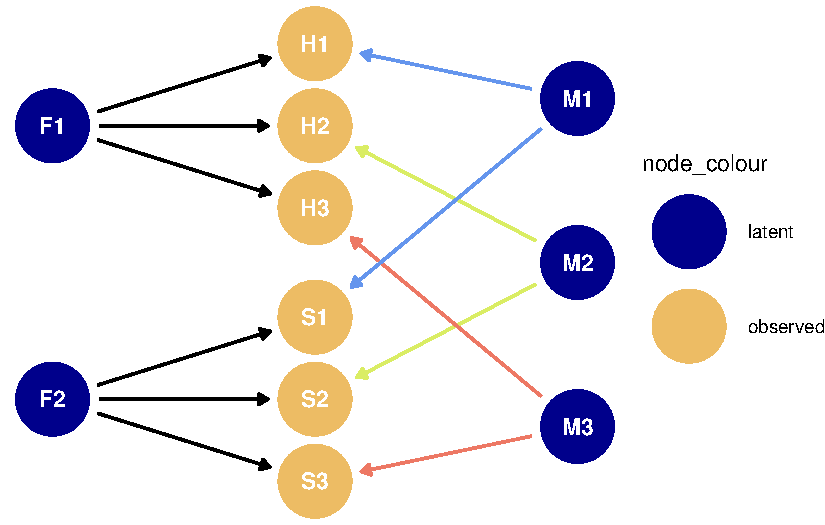
\includegraphics{./mtmm-and-error-structure-modelling_files/figure-pdf/unnamed-chunk-2-1.pdf}

}

\end{figure}

See how the measurment effects M1, M2, and M3 each create a backdoor
path between the two factors F1 and F2. So if I want to get
better-seeming (and, under the DAG, more accurate) estimate of
between-factor correlation, then I need to find a way to close those
backdoor paths. The classic way to close these paths would be to
condition on the measurement effects by adding them to the linear model,
but I can't directly do this because they are unmeasured. But, as
discussed above, I can still sort of do it by adding them as factors to
my CFA model, or by freely estimating residual correlation between the
observed variables that share a measurement approach, which should work
if my DAG is mostly accurate.

Unfortunately, the authors of this paper haven't published their data.
But we can take this as an opportunity to practice simulating a dataset
with relationships implied by a DAG.

\begin{Shaded}
\begin{Highlighting}[]
\DocumentationTok{\#\#\# Simulate Data from the DAG}

\CommentTok{\# Set seed for replicable results}
\FunctionTok{set.seed}\NormalTok{(}\DecValTok{233}\NormalTok{)}

\CommentTok{\# Set sample size}
\NormalTok{N }\OtherTok{\textless{}{-}} \DecValTok{305}

\CommentTok{\# Create the dataset}
\NormalTok{dat\_fake }\OtherTok{\textless{}{-}} \FunctionTok{tibble}\NormalTok{(}
  
  \CommentTok{\# The factors are uncorrelated in reality, but}
  \CommentTok{\# will be confounded by the measurement effects!}
  \AttributeTok{F1 =} \FunctionTok{rnorm}\NormalTok{(N, }\DecValTok{0}\NormalTok{, }\DecValTok{1}\NormalTok{),}
  \AttributeTok{F2 =} \FunctionTok{rnorm}\NormalTok{(N, }\DecValTok{0}\NormalTok{, }\DecValTok{1}\NormalTok{),}
  
  \CommentTok{\# The measurement effects}
  \AttributeTok{M1 =} \FunctionTok{rnorm}\NormalTok{(N, }\DecValTok{0}\NormalTok{, }\DecValTok{1}\NormalTok{),}
  \AttributeTok{M2 =} \FunctionTok{rnorm}\NormalTok{(N, }\DecValTok{0}\NormalTok{, }\DecValTok{1}\NormalTok{),}
  \AttributeTok{M3 =} \FunctionTok{rnorm}\NormalTok{(N, }\DecValTok{0}\NormalTok{, }\DecValTok{1}\NormalTok{),}
  
  \CommentTok{\# The DAG says the measurements are fully determined by the latent factors and measurement effects}
  \AttributeTok{H1 =}\NormalTok{ .}\DecValTok{8}\SpecialCharTok{*}\NormalTok{F1 }\SpecialCharTok{+} \FloatTok{0.7}\SpecialCharTok{*}\NormalTok{M1 }\SpecialCharTok{+} \FunctionTok{rnorm}\NormalTok{(N, }\DecValTok{0}\NormalTok{, .}\DecValTok{3}\NormalTok{),}
  \AttributeTok{H2 =}\NormalTok{ .}\DecValTok{7}\SpecialCharTok{*}\NormalTok{F1 }\SpecialCharTok{+} \FloatTok{0.7}\SpecialCharTok{*}\NormalTok{M2 }\SpecialCharTok{+} \FunctionTok{rnorm}\NormalTok{(N, }\DecValTok{0}\NormalTok{, .}\DecValTok{3}\NormalTok{),}
  \AttributeTok{H3 =}\NormalTok{ .}\DecValTok{9}\SpecialCharTok{*}\NormalTok{F1 }\SpecialCharTok{+} \FloatTok{0.7}\SpecialCharTok{*}\NormalTok{M3 }\SpecialCharTok{+} \FunctionTok{rnorm}\NormalTok{(N, }\DecValTok{0}\NormalTok{, .}\DecValTok{3}\NormalTok{),}
  \AttributeTok{S1 =}\NormalTok{ .}\DecValTok{8}\SpecialCharTok{*}\NormalTok{F2 }\SpecialCharTok{+} \FloatTok{0.7}\SpecialCharTok{*}\NormalTok{M1 }\SpecialCharTok{+} \FunctionTok{rnorm}\NormalTok{(N, }\DecValTok{0}\NormalTok{, .}\DecValTok{3}\NormalTok{),}
  \AttributeTok{S2 =}\NormalTok{ .}\DecValTok{7}\SpecialCharTok{*}\NormalTok{F2 }\SpecialCharTok{+} \FloatTok{0.7}\SpecialCharTok{*}\NormalTok{M2 }\SpecialCharTok{+} \FunctionTok{rnorm}\NormalTok{(N, }\DecValTok{0}\NormalTok{, .}\DecValTok{3}\NormalTok{),}
  \AttributeTok{S3 =}\NormalTok{ .}\DecValTok{9}\SpecialCharTok{*}\NormalTok{F2 }\SpecialCharTok{+} \FloatTok{0.7}\SpecialCharTok{*}\NormalTok{M3 }\SpecialCharTok{+} \FunctionTok{rnorm}\NormalTok{(N, }\DecValTok{0}\NormalTok{, .}\DecValTok{3}\NormalTok{) }
\NormalTok{) }
\end{Highlighting}
\end{Shaded}

Fun! Now we have our fake data to play with. For starters, since we
actually \emph{do} have the values of the latent variables in our
dataset, we can demonstrate how directly controlling for the measurement
effects in a regression model can close the backdoor path between the
factors.

\begin{Shaded}
\begin{Highlighting}[]
\FunctionTok{list}\NormalTok{(}
  \FunctionTok{lm}\NormalTok{(H1 }\SpecialCharTok{\textasciitilde{}}\NormalTok{ S1, dat\_fake), }
  \FunctionTok{lm}\NormalTok{(H1 }\SpecialCharTok{\textasciitilde{}}\NormalTok{ S1 }\SpecialCharTok{+}\NormalTok{ M1, dat\_fake)}
\NormalTok{) }\SpecialCharTok{\%\textgreater{}\%} 
  
  \FunctionTok{map}\NormalTok{(broom}\SpecialCharTok{::}\NormalTok{tidy) }\SpecialCharTok{\%\textgreater{}\%} 
  
\NormalTok{  knitr}\SpecialCharTok{::}\FunctionTok{kable}\NormalTok{()}
\end{Highlighting}
\end{Shaded}

\begin{table}

\centering
\begin{tabular}[t]{l|r|r|r|r}
\hline
term & estimate & std.error & statistic & p.value\\
\hline
(Intercept) & 0.0249271 & 0.0572795 & 0.435184 & 0.6637387\\
\hline
S1 & 0.4555127 & 0.0491323 & 9.271137 & 0.0000000\\
\hline
\end{tabular}
\centering
\begin{tabular}[t]{l|r|r|r|r}
\hline
term & estimate & std.error & statistic & p.value\\
\hline
(Intercept) & 0.0466841 & 0.0456881 & 1.0217995 & 0.3076936\\
\hline
S1 & -0.0137610 & 0.0528505 & -0.2603763 & 0.7947509\\
\hline
M1 & 0.7636731 & 0.0577500 & 13.2237680 & 0.0000000\\
\hline
\end{tabular}
\end{table}

When we just do the simple regression of H1 on S1 we get a big effect
with a highly statistically significant p-value, despite the fact that
we \emph{know} there's no causal relationship there! But then when we
include the confounding measurement effect in the model this effect
vanishes in smoke.

That's all well and good. But in reality we won't have measurements of
the latent variables, so we won't be able to directly control for them.
Thankfully, we have Factor Analysis. We can control for the measurement
effects by estimating the residual correlation between each pair of
variables that share a measurement effect. Since, under the DAG, the
measurement effects are the only source of correlation between these
variables, this should close the backdoor path, IE we should get
unbiased estimates of the factor loadings.

\ldots.@Brown2006 calls this an ``error theory''\ldots..

\hypertarget{correlated-uniqueness-model}{%
\subsection*{Correlated Uniqueness
Model}\label{correlated-uniqueness-model}}
\addcontentsline{toc}{subsection}{Correlated Uniqueness Model}

To illustrate, we'll fit 2 models: The first is a basic CFA model that
just loads each measured variable on its corresponding factor. The
second specifies that the residual correlation between the
measurement-confounded variables should be freely estimated, IE not
fixed at 0.

First let's define our utility function like we did in the previous
chapter:

\begin{Shaded}
\begin{Highlighting}[]
\DocumentationTok{\#\#\# Define a custom function}
\NormalTok{fit\_measures }\OtherTok{\textless{}{-}} \ControlFlowTok{function}\NormalTok{(fit)\{}
  
\NormalTok{  summary }\OtherTok{\textless{}{-}} \FunctionTok{summary}\NormalTok{(fit, }\AttributeTok{fit.measures =} \ConstantTok{TRUE}\NormalTok{, }\AttributeTok{standardized =} \ConstantTok{TRUE}\NormalTok{)}
  
\NormalTok{  res }\OtherTok{\textless{}{-}} \FunctionTok{list}\NormalTok{(}
    
    \CommentTok{\# Chi{-}Squared}
    \AttributeTok{chi\_squared =} \FunctionTok{tibble}\NormalTok{(}
      \AttributeTok{Test             =} \StringTok{"standard chi{-}squared"}\NormalTok{,}
      \StringTok{\textasciigrave{}}\AttributeTok{DF}\StringTok{\textasciigrave{}}             \OtherTok{=}\NormalTok{ summary}\SpecialCharTok{$}\NormalTok{test}\SpecialCharTok{$}\NormalTok{standard}\SpecialCharTok{$}\NormalTok{df,}
      \StringTok{\textasciigrave{}}\AttributeTok{Test Statistic}\StringTok{\textasciigrave{}} \OtherTok{=} \FunctionTok{round}\NormalTok{(summary}\SpecialCharTok{$}\NormalTok{test}\SpecialCharTok{$}\NormalTok{standard}\SpecialCharTok{$}\NormalTok{stat, }\DecValTok{2}\NormalTok{),}
      \StringTok{\textasciigrave{}}\AttributeTok{p{-}value}\StringTok{\textasciigrave{}}        \OtherTok{=}\NormalTok{ summary}\SpecialCharTok{$}\NormalTok{test}\SpecialCharTok{$}\NormalTok{standard}\SpecialCharTok{$}\NormalTok{pvalue) }\SpecialCharTok{\%\textgreater{}\%} 
      
      \FunctionTok{mutate}\NormalTok{(}\FunctionTok{across}\NormalTok{(}\FunctionTok{everything}\NormalTok{(), as.character)) }\SpecialCharTok{\%\textgreater{}\%} 
      
      \FunctionTok{pivot\_longer}\NormalTok{(}\FunctionTok{everything}\NormalTok{()),}
    
    \CommentTok{\# RMSEA}
    \AttributeTok{rmsea =}\NormalTok{ summary}\SpecialCharTok{$}\NormalTok{fit }\SpecialCharTok{\%\textgreater{}\%} 
      
      \FunctionTok{as\_tibble}\NormalTok{(}\AttributeTok{rownames =} \StringTok{"stat"}\NormalTok{) }\SpecialCharTok{\%\textgreater{}\%} 
      
      \FunctionTok{filter}\NormalTok{(}\FunctionTok{str\_detect}\NormalTok{(stat, }\StringTok{"rmsea"}\NormalTok{)),}
    
    \CommentTok{\# CFI and TLI}
    \AttributeTok{cfi\_tli =}\NormalTok{ summary}\SpecialCharTok{$}\NormalTok{fit }\SpecialCharTok{\%\textgreater{}\%} 
      
      \FunctionTok{as\_tibble}\NormalTok{(}\AttributeTok{rownames =} \StringTok{"stat"}\NormalTok{) }\SpecialCharTok{\%\textgreater{}\%} 
      
      \FunctionTok{filter}\NormalTok{(}\FunctionTok{str\_detect}\NormalTok{(stat, }\StringTok{"cfi|tli"}\NormalTok{)) }
    
\NormalTok{  )}
  
\NormalTok{  res}
  
\NormalTok{\}}
\end{Highlighting}
\end{Shaded}

\begin{Shaded}
\begin{Highlighting}[]
\NormalTok{basic.definition }\OtherTok{\textless{}{-}} 
  \StringTok{\textquotesingle{}happy =\textasciitilde{} H1 + H2 + H3}
\StringTok{   sad =\textasciitilde{} S1 + S2 + S3}
\StringTok{   \textquotesingle{}}

\NormalTok{correlated\_uniqueness.definition }\OtherTok{\textless{}{-}} 
  \StringTok{\textquotesingle{}happy =\textasciitilde{} H1 + H2 + H3}
\StringTok{   sad =\textasciitilde{} S1 + S2 + S3}
\StringTok{   }
\StringTok{   H1 \textasciitilde{}\textasciitilde{} S1}
\StringTok{   H2 \textasciitilde{}\textasciitilde{} S2}
\StringTok{   H3 \textasciitilde{}\textasciitilde{} S3}
\StringTok{   \textquotesingle{}}
\NormalTok{basic.fit }\OtherTok{\textless{}{-}} \FunctionTok{cfa}\NormalTok{(}
  \AttributeTok{data =}\NormalTok{ dat\_fake }\SpecialCharTok{\%\textgreater{}\%} \FunctionTok{select}\NormalTok{(}\FunctionTok{matches}\NormalTok{(}\StringTok{"\^{}(H|S)"}\NormalTok{)),}
  \AttributeTok{model =}\NormalTok{ basic.definition}
\NormalTok{)}

\NormalTok{correlated\_uniqueness.fit }\OtherTok{\textless{}{-}} \FunctionTok{cfa}\NormalTok{(}
  \AttributeTok{data =}\NormalTok{ dat\_fake }\SpecialCharTok{\%\textgreater{}\%} \FunctionTok{select}\NormalTok{(}\FunctionTok{matches}\NormalTok{(}\StringTok{"\^{}(H|S)"}\NormalTok{)),}
  \AttributeTok{model =}\NormalTok{ correlated\_uniqueness.definition}
\NormalTok{)}

\NormalTok{summary.basic.fit }\OtherTok{\textless{}{-}} \FunctionTok{summary}\NormalTok{(basic.fit, }\AttributeTok{standardized =} \ConstantTok{TRUE}\NormalTok{)}
\NormalTok{summary.correlated\_uniqueness.fit }\OtherTok{\textless{}{-}} \FunctionTok{summary}\NormalTok{(correlated\_uniqueness.fit, }\AttributeTok{standardized =} \ConstantTok{TRUE}\NormalTok{)}

\NormalTok{summary.basic.fit}
\end{Highlighting}
\end{Shaded}

\begin{verbatim}
lavaan 0.6.16 ended normally after 23 iterations

  Estimator                                         ML
  Optimization method                           NLMINB
  Number of model parameters                        13

  Number of observations                           305

Model Test User Model:
                                                      
  Test statistic                               802.905
  Degrees of freedom                                 8
  P-value (Chi-square)                           0.000

Parameter Estimates:

  Standard errors                             Standard
  Information                                 Expected
  Information saturated (h1) model          Structured

Latent Variables:
                   Estimate  Std.Err  z-value  P(>|z|)   Std.lv  Std.all
  happy =~                                                              
    H1                1.000                               0.816    0.723
    H2                0.741    0.090    8.236    0.000    0.605    0.615
    H3                1.044    0.123    8.496    0.000    0.852    0.741
  sad =~                                                                
    S1                1.000                               0.906    0.778
    S2                0.818    0.079   10.302    0.000    0.742    0.704
    S3                0.980    0.093   10.522    0.000    0.888    0.752

Covariances:
                   Estimate  Std.Err  z-value  P(>|z|)   Std.lv  Std.all
  happy ~~                                                              
    sad               0.236    0.060    3.934    0.000    0.319    0.319

Variances:
                   Estimate  Std.Err  z-value  P(>|z|)   Std.lv  Std.all
   .H1                0.609    0.084    7.214    0.000    0.609    0.478
   .H2                0.601    0.062    9.662    0.000    0.601    0.621
   .H3                0.597    0.089    6.721    0.000    0.597    0.451
   .S1                0.537    0.077    6.989    0.000    0.537    0.395
   .S2                0.560    0.062    8.964    0.000    0.560    0.505
   .S3                0.604    0.078    7.726    0.000    0.604    0.434
    happy             0.667    0.114    5.860    0.000    1.000    1.000
    sad               0.822    0.119    6.886    0.000    1.000    1.000
\end{verbatim}

\begin{Shaded}
\begin{Highlighting}[]
\NormalTok{summary.correlated\_uniqueness.fit}
\end{Highlighting}
\end{Shaded}

\begin{verbatim}
lavaan 0.6.16 ended normally after 47 iterations

  Estimator                                         ML
  Optimization method                           NLMINB
  Number of model parameters                        16

  Number of observations                           305

Model Test User Model:
                                                      
  Test statistic                                13.448
  Degrees of freedom                                 5
  P-value (Chi-square)                           0.020

Parameter Estimates:

  Standard errors                             Standard
  Information                                 Expected
  Information saturated (h1) model          Structured

Latent Variables:
                   Estimate  Std.Err  z-value  P(>|z|)   Std.lv  Std.all
  happy =~                                                              
    H1                1.000                               0.738    0.669
    H2                0.915    0.055   16.787    0.000    0.676    0.657
    H3                1.157    0.066   17.625    0.000    0.854    0.755
  sad =~                                                                
    S1                1.000                               0.866    0.744
    S2                0.863    0.042   20.433    0.000    0.747    0.724
    S3                1.057    0.048   21.972    0.000    0.915    0.761

Covariances:
                   Estimate  Std.Err  z-value  P(>|z|)   Std.lv  Std.all
 .H1 ~~                                                                 
   .S1                0.551    0.061    9.007    0.000    0.551    0.866
 .H2 ~~                                                                 
   .S2                0.458    0.051    8.973    0.000    0.458    0.831
 .H3 ~~                                                                 
   .S3                0.501    0.062    8.133    0.000    0.501    0.868
  happy ~~                                                              
    sad               0.032    0.050    0.638    0.524    0.050    0.050

Variances:
                   Estimate  Std.Err  z-value  P(>|z|)   Std.lv  Std.all
   .H1                0.672    0.070    9.641    0.000    0.672    0.552
   .H2                0.600    0.061    9.813    0.000    0.600    0.568
   .H3                0.550    0.071    7.769    0.000    0.550    0.430
   .S1                0.604    0.066    9.121    0.000    0.604    0.446
   .S2                0.507    0.053    9.538    0.000    0.507    0.476
   .S3                0.607    0.069    8.789    0.000    0.607    0.420
    happy             0.545    0.073    7.450    0.000    1.000    1.000
    sad               0.749    0.086    8.762    0.000    1.000    1.000
\end{verbatim}

\begin{Shaded}
\begin{Highlighting}[]
\FunctionTok{fit\_measures}\NormalTok{(basic.fit) }\SpecialCharTok{\%\textgreater{}\%} 
  
\NormalTok{  knitr}\SpecialCharTok{::}\FunctionTok{kable}\NormalTok{(}\AttributeTok{caption =} \StringTok{"Basic Model"}\NormalTok{)}
\end{Highlighting}
\end{Shaded}

\begin{table}
\caption{Basic Model}

\centering
\begin{tabular}[t]{l|l}
\hline
name & value\\
\hline
Test & standard chi-squared\\
\hline
DF & 8\\
\hline
Test Statistic & 802.9\\
\hline
p-value & 0\\
\hline
\end{tabular}
\centering
\begin{tabular}[t]{l|r}
\hline
stat & value\\
\hline
rmsea & 0.5707720\\
\hline
rmsea.ci.lower & 0.5377551\\
\hline
rmsea.ci.upper & 0.6044999\\
\hline
rmsea.ci.level & 0.9000000\\
\hline
rmsea.pvalue & 0.0000000\\
\hline
rmsea.close.h0 & 0.0500000\\
\hline
rmsea.notclose.pvalue & 1.0000000\\
\hline
rmsea.notclose.h0 & 0.0800000\\
\hline
\end{tabular}
\centering
\begin{tabular}[t]{l|r}
\hline
stat & value\\
\hline
cfi & 0.3742618\\
\hline
tli & -0.1732591\\
\hline
\end{tabular}
\end{table}

\begin{Shaded}
\begin{Highlighting}[]
\FunctionTok{fit\_measures}\NormalTok{(correlated\_uniqueness.fit) }\SpecialCharTok{\%\textgreater{}\%} 
  
\NormalTok{  knitr}\SpecialCharTok{::}\FunctionTok{kable}\NormalTok{(}\AttributeTok{caption =} \StringTok{"Correlated Uniqueness Model"}\NormalTok{)}
\end{Highlighting}
\end{Shaded}

\begin{table}
\caption{Correlated Uniqueness Model}

\centering
\begin{tabular}[t]{l|l}
\hline
name & value\\
\hline
Test & standard chi-squared\\
\hline
DF & 5\\
\hline
Test Statistic & 13.45\\
\hline
p-value & 0.0195200124719597\\
\hline
\end{tabular}
\centering
\begin{tabular}[t]{l|r}
\hline
stat & value\\
\hline
rmsea & 0.07443086\\
\hline
rmsea.ci.lower & 0.02734066\\
\hline
rmsea.ci.upper & 0.12377511\\
\hline
rmsea.ci.level & 0.90000000\\
\hline
rmsea.pvalue & 0.16609111\\
\hline
rmsea.close.h0 & 0.05000000\\
\hline
rmsea.notclose.pvalue & 0.47823144\\
\hline
rmsea.notclose.h0 & 0.08000000\\
\hline
\end{tabular}
\centering
\begin{tabular}[t]{l|r}
\hline
stat & value\\
\hline
cfi & 0.9933495\\
\hline
tli & 0.9800485\\
\hline
\end{tabular}
\end{table}

Here we see that under the basic model we have some moderate correlation
between the \texttt{happy} and \texttt{sad} factors, which is a bit of a
murky result: it doesn't tell us one way or the other whether happiness
and sadness are separate constructs I can feel together or two extremes
of the same feeling. But under the correlated uniqueness model this
correlation evaporates because we've controlled for the measurement
effects, closing the backdoor path between \texttt{happy} and
\texttt{sad}. This model also greatly improves goodness-of-fit, which
makes sense because it better reflects the true data-generating process
we coded up.

We also could have controlled for the measurement effects by including
measurement factors, IE by adopting a `Correlated Methods Model'. I
tried this but I actually I couldn't get this model to converge,
regardless of whether its method factors were correlated or uncorrelated
(an `Uncorrelated Methods Model'. Brown (2006) actually mentions this as
a common issue, and favours the Correlated Uniqueness Model for that
reason. In his words:

\begin{quote}
``an overriding drawback of the correlated methods model is that it is
usually empirically underidentified. Consequently, a correlated methods
solution will typically fail to converge. If it does converge, the
solution will usually be associated with Heywood cases {[}negative
variance estimates{]} and large standard errors''
\end{quote}

Now let's consider the other case in which measurement effects might be
hurting us: the case in which \emph{within}-factor measurements are
confounded by measurement effects. Here's the DAG:

\begin{Shaded}
\begin{Highlighting}[]
\NormalTok{dag\_coords }\OtherTok{\textless{}{-}} \FunctionTok{list}\NormalTok{(}
  \AttributeTok{x =} \FunctionTok{c}\NormalTok{(}
    \AttributeTok{F1 =} \DecValTok{1}\NormalTok{, }
    \AttributeTok{F2 =} \DecValTok{1}\NormalTok{,}
    \AttributeTok{H1 =} \DecValTok{2}\NormalTok{,}
    \AttributeTok{H2 =} \DecValTok{2}\NormalTok{,}
    \AttributeTok{H3 =} \DecValTok{2}\NormalTok{,}
    \AttributeTok{S1 =} \DecValTok{2}\NormalTok{,}
    \AttributeTok{S2 =} \DecValTok{2}\NormalTok{,}
    \AttributeTok{S3 =} \DecValTok{2}\NormalTok{,}
    \AttributeTok{M1 =} \DecValTok{3}\NormalTok{,}
    \AttributeTok{M2 =} \DecValTok{3}\NormalTok{),}
  \AttributeTok{y =} \FunctionTok{c}\NormalTok{(}
    \AttributeTok{F1 =} \FloatTok{2.5}\NormalTok{,}
    \AttributeTok{F2 =} \FloatTok{1.5}\NormalTok{,}
    \AttributeTok{H1 =} \FloatTok{2.8}\NormalTok{,}
    \AttributeTok{H2 =} \FloatTok{2.5}\NormalTok{,}
    \AttributeTok{H3 =} \FloatTok{2.2}\NormalTok{,}
    \AttributeTok{S1 =} \FloatTok{1.8}\NormalTok{,}
    \AttributeTok{S2 =} \FloatTok{1.5}\NormalTok{,}
    \AttributeTok{S3 =} \FloatTok{1.2}\NormalTok{,}
    \AttributeTok{M1 =} \FloatTok{2.5}\NormalTok{,}
    \AttributeTok{M2 =} \FloatTok{1.5}
\NormalTok{  )}
\NormalTok{)}

\CommentTok{\# Set DAG relationships and aesthetics}
\NormalTok{measurement\_confounding\_dag }\OtherTok{\textless{}{-}}\NormalTok{ ggdag}\SpecialCharTok{::}\FunctionTok{dagify}\NormalTok{(}
\NormalTok{  H3 }\SpecialCharTok{\textasciitilde{}}\NormalTok{ F1,}
\NormalTok{  S2 }\SpecialCharTok{\textasciitilde{}}\NormalTok{ F2,}
\NormalTok{  H1 }\SpecialCharTok{\textasciitilde{}}\NormalTok{ M1,}
\NormalTok{  H2 }\SpecialCharTok{\textasciitilde{}}\NormalTok{ M1,}
\NormalTok{  H3 }\SpecialCharTok{\textasciitilde{}}\NormalTok{ M1,}
\NormalTok{  S1 }\SpecialCharTok{\textasciitilde{}}\NormalTok{ M2,}
\NormalTok{  S2 }\SpecialCharTok{\textasciitilde{}}\NormalTok{ M2,}
\NormalTok{  S3 }\SpecialCharTok{\textasciitilde{}}\NormalTok{ M2,}
  \AttributeTok{coords =}\NormalTok{ dag\_coords}
\NormalTok{) }\SpecialCharTok{\%\textgreater{}\%} 
  
  \FunctionTok{tidy\_dagitty}\NormalTok{() }\SpecialCharTok{\%\textgreater{}\%} 
  
  \FunctionTok{mutate}\NormalTok{(}
    
    \AttributeTok{node\_colour =} \FunctionTok{case\_when}\NormalTok{(}
      \FunctionTok{grepl}\NormalTok{(}\StringTok{"\^{}F|M"}\NormalTok{, name) }\SpecialCharTok{\textasciitilde{}} \StringTok{"latent"}\NormalTok{,}
      \FunctionTok{grepl}\NormalTok{(}\StringTok{"\^{}H|S"}\NormalTok{, name) }\SpecialCharTok{\textasciitilde{}} \StringTok{"observed"}
\NormalTok{    ),}
    
    \AttributeTok{edge\_colour =} \FunctionTok{case\_when}\NormalTok{(}
      \FunctionTok{grepl}\NormalTok{(}\StringTok{"M1"}\NormalTok{, name)  }\SpecialCharTok{\textasciitilde{}} \StringTok{"cornflower blue"}\NormalTok{,}
      \FunctionTok{grepl}\NormalTok{(}\StringTok{"M2"}\NormalTok{, name) }\SpecialCharTok{\textasciitilde{}} \StringTok{"\#ed7864"}\NormalTok{,}
      \FunctionTok{grepl}\NormalTok{(}\StringTok{"\^{}XX"}\NormalTok{, name) }\SpecialCharTok{\&} \FunctionTok{grepl}\NormalTok{(}\StringTok{"3$"}\NormalTok{, to) }\SpecialCharTok{\textasciitilde{}} \StringTok{"\#ed7864"}\NormalTok{,}
      \FunctionTok{grepl}\NormalTok{(}\StringTok{"\^{}F"}\NormalTok{, name)                   }\SpecialCharTok{\textasciitilde{}} \StringTok{"black"}
\NormalTok{    )}
\NormalTok{  )}

\CommentTok{\# Plot the DAG}
\NormalTok{measurement\_confounding\_dag }\SpecialCharTok{\%\textgreater{}\%}
  \FunctionTok{ggplot}\NormalTok{(}\FunctionTok{aes}\NormalTok{(}\AttributeTok{x =}\NormalTok{ x, }\AttributeTok{y =}\NormalTok{ y, }\AttributeTok{xend =}\NormalTok{ xend, }\AttributeTok{yend =}\NormalTok{ yend)) }\SpecialCharTok{+}
  \FunctionTok{geom\_dag\_point}\NormalTok{(}\FunctionTok{aes}\NormalTok{(}\AttributeTok{colour =}\NormalTok{ node\_colour)) }\SpecialCharTok{+}
  \FunctionTok{scale\_colour\_manual}\NormalTok{(}\AttributeTok{values =} \FunctionTok{c}\NormalTok{(}\StringTok{"dark blue"}\NormalTok{, }\StringTok{"\#edbc64"}\NormalTok{)) }\SpecialCharTok{+} 
  \FunctionTok{geom\_dag\_edges}\NormalTok{(}\FunctionTok{aes}\NormalTok{(}\AttributeTok{edge\_colour =}\NormalTok{ edge\_colour)) }\SpecialCharTok{+}
  \FunctionTok{geom\_dag\_text}\NormalTok{() }\SpecialCharTok{+}
  \FunctionTok{theme\_void}\NormalTok{()}
\end{Highlighting}
\end{Shaded}

\begin{figure}[H]

{\centering 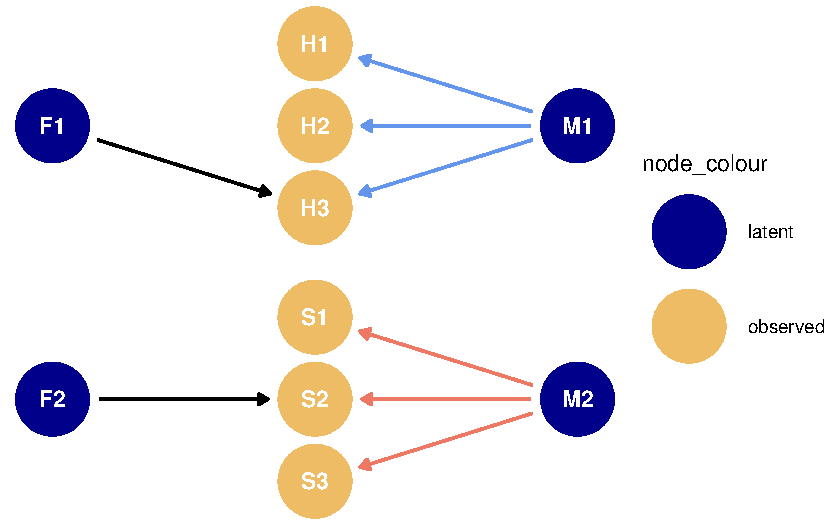
\includegraphics{./mtmm-and-error-structure-modelling_files/figure-pdf/unnamed-chunk-7-1.pdf}

}

\end{figure}

This is the `true' data-generating process we'll be simulating data from
in a moment. Notice that even though the researcher (who can't see this
DAG) might think that the unobseved factor causally influences all 3
measured variables, the reality is that each factor only influences one
of the measured variables. However, the purported within-factor
variables are confounded by measurement method.

Let's simulate the data and analyze:

\begin{Shaded}
\begin{Highlighting}[]
\CommentTok{\# Set seed for replicable results}
\FunctionTok{set.seed}\NormalTok{(}\DecValTok{233}\NormalTok{)}

\CommentTok{\# Set sample size}
\NormalTok{N }\OtherTok{\textless{}{-}} \DecValTok{30000}

\CommentTok{\# Create the dataset}
\NormalTok{dat\_fake }\OtherTok{\textless{}{-}} \FunctionTok{tibble}\NormalTok{(}
  
  \CommentTok{\# Create some uncorrelated factors}
  \AttributeTok{F1 =} \FunctionTok{rnorm}\NormalTok{(N, }\DecValTok{0}\NormalTok{, }\DecValTok{1}\NormalTok{),}
  \AttributeTok{F2 =} \FunctionTok{rnorm}\NormalTok{(N, }\DecValTok{0}\NormalTok{, }\DecValTok{1}\NormalTok{),}
  
  \CommentTok{\# Create some measurement effects}
  \AttributeTok{M1 =} \FunctionTok{rnorm}\NormalTok{(N, }\DecValTok{0}\NormalTok{, }\DecValTok{1}\NormalTok{),}
  \AttributeTok{M2 =} \FunctionTok{rnorm}\NormalTok{(N, }\DecValTok{0}\NormalTok{, }\DecValTok{1}\NormalTok{),}
  
  \CommentTok{\# The DAG says only H3 and S2 are influenced by the factors, but all variables are influenced by a measurement effect.}
  \AttributeTok{H1 =} \FloatTok{0.7}\SpecialCharTok{*}\NormalTok{M1 }\SpecialCharTok{+} \FunctionTok{rnorm}\NormalTok{(N, }\DecValTok{0}\NormalTok{, .}\DecValTok{3}\NormalTok{),}
  \AttributeTok{H2 =} \FloatTok{0.8}\SpecialCharTok{*}\NormalTok{M1 }\SpecialCharTok{+} \FunctionTok{rnorm}\NormalTok{(N, }\DecValTok{0}\NormalTok{, .}\DecValTok{3}\NormalTok{),}
  \AttributeTok{H3 =} \FloatTok{0.9}\SpecialCharTok{*}\NormalTok{F1 }\SpecialCharTok{+} \FloatTok{0.8}\SpecialCharTok{*}\NormalTok{M1 }\SpecialCharTok{+} \FunctionTok{rnorm}\NormalTok{(N, }\DecValTok{0}\NormalTok{, .}\DecValTok{3}\NormalTok{),}
  \AttributeTok{S1 =} \FloatTok{0.7}\SpecialCharTok{*}\NormalTok{M2 }\SpecialCharTok{+} \FunctionTok{rnorm}\NormalTok{(N, }\DecValTok{0}\NormalTok{, .}\DecValTok{3}\NormalTok{),}
  \AttributeTok{S2 =} \FloatTok{0.7}\SpecialCharTok{*}\NormalTok{F2 }\SpecialCharTok{+} \FloatTok{0.8}\SpecialCharTok{*}\NormalTok{M2 }\SpecialCharTok{+} \FunctionTok{rnorm}\NormalTok{(N, }\DecValTok{0}\NormalTok{, .}\DecValTok{3}\NormalTok{),}
  \AttributeTok{S3 =} \FloatTok{0.7}\SpecialCharTok{*}\NormalTok{M2 }\SpecialCharTok{+} \FunctionTok{rnorm}\NormalTok{(N, }\DecValTok{0}\NormalTok{, .}\DecValTok{3}\NormalTok{) }
\NormalTok{) }
\end{Highlighting}
\end{Shaded}

First let's fit a basic naive CFA model that does the standard thing of
keeping the covariances between variables fixed at 0. Based on the DAG,
we should expect this model to return a strong (publishable) but
misleading answer -- it will notice the correlation between variables
that are considered within-factor under our hypothesis, and say `wow so
correlated, that's consistent with them being \emph{caused} by that
factor'. But we know this is wrong: their correlation is simply driven
by the shared measurement method:

\begin{Shaded}
\begin{Highlighting}[]
\NormalTok{basic.definition }\OtherTok{\textless{}{-}} 
  \StringTok{\textquotesingle{}happy =\textasciitilde{} H1 + H2 + H3}
\StringTok{   sad =\textasciitilde{} S1 + S2 + S3}
\StringTok{   \textquotesingle{}}

\NormalTok{basic.fit }\OtherTok{\textless{}{-}} \FunctionTok{cfa}\NormalTok{(}
  \AttributeTok{data =}\NormalTok{ dat\_fake,}
  \AttributeTok{model =}\NormalTok{ basic.definition}
\NormalTok{)}

\FunctionTok{summary}\NormalTok{(basic.fit, }\AttributeTok{standardized =} \ConstantTok{TRUE}\NormalTok{)}
\end{Highlighting}
\end{Shaded}

\begin{verbatim}
lavaan 0.6.16 ended normally after 25 iterations

  Estimator                                         ML
  Optimization method                           NLMINB
  Number of model parameters                        13

  Number of observations                         30000

Model Test User Model:
                                                      
  Test statistic                                 7.086
  Degrees of freedom                                 8
  P-value (Chi-square)                           0.527

Parameter Estimates:

  Standard errors                             Standard
  Information                                 Expected
  Information saturated (h1) model          Structured

Latent Variables:
                   Estimate  Std.Err  z-value  P(>|z|)   Std.lv  Std.all
  happy =~                                                              
    H1                1.000                               0.705    0.920
    H2                1.141    0.006  196.951    0.000    0.804    0.936
    H3                1.142    0.009  129.172    0.000    0.805    0.646
  sad =~                                                                
    S1                1.000                               0.696    0.917
    S2                1.142    0.008  151.721    0.000    0.795    0.722
    S3                1.004    0.005  206.981    0.000    0.699    0.922

Covariances:
                   Estimate  Std.Err  z-value  P(>|z|)   Std.lv  Std.all
  happy ~~                                                              
    sad              -0.002    0.003   -0.765    0.444   -0.005   -0.005

Variances:
                   Estimate  Std.Err  z-value  P(>|z|)   Std.lv  Std.all
   .H1                0.090    0.002   42.749    0.000    0.090    0.154
   .H2                0.091    0.003   34.103    0.000    0.091    0.124
   .H3                0.903    0.008  115.595    0.000    0.903    0.582
   .S1                0.091    0.002   49.153    0.000    0.091    0.158
   .S2                0.581    0.005  110.971    0.000    0.581    0.479
   .S3                0.086    0.002   46.614    0.000    0.086    0.150
    happy             0.497    0.005   96.783    0.000    1.000    1.000
    sad               0.484    0.005   98.040    0.000    1.000    1.000
\end{verbatim}

And there you have it -- just as foretold, we have super strong factor
loadings for all the variables, even those that are not actually
causally influenced by the factor! So it may \emph{look} like I have
strong convergent validity, but hopefully if we try to publish this, a
reviewer will raise the possibility that these correlations are
confounded by measurement effects.

Now I'm going to try closing the backdoor paths between the
non-factor-caused variables by allowing the model to learn the
covariances, thereby hopefully controlling for unobserved sources of
confounding (like the measurement effect). If the loadings stay strong,
then my claims to convergent validity are more reasonable.

\begin{Shaded}
\begin{Highlighting}[]
\NormalTok{correlated\_uniqueness.definition }\OtherTok{\textless{}{-}} 
  \StringTok{\textquotesingle{}happy =\textasciitilde{} H1 + H2 + H3}
\StringTok{   sad   =\textasciitilde{} S1 + S2 + S3}
\StringTok{   }
\StringTok{   H1 \textasciitilde{}\textasciitilde{} H2}
\StringTok{   H1 \textasciitilde{}\textasciitilde{} H3}
\StringTok{   H2 \textasciitilde{}\textasciitilde{} H3}
\StringTok{   S1 \textasciitilde{}\textasciitilde{} S2}
\StringTok{   S1 \textasciitilde{}\textasciitilde{} S3}
\StringTok{   S2 \textasciitilde{}\textasciitilde{} S3}
\StringTok{   \textquotesingle{}}

\NormalTok{correlated\_uniqueness.fit }\OtherTok{\textless{}{-}} \FunctionTok{cfa}\NormalTok{(}
  \AttributeTok{data =}\NormalTok{ dat\_fake,}
  \AttributeTok{model =}\NormalTok{ correlated\_uniqueness.definition}
\NormalTok{)}
\end{Highlighting}
\end{Shaded}

\begin{verbatim}
Warning in lav_model_vcov(lavmodel = lavmodel, lavsamplestats = lavsamplestats, : lavaan WARNING:
    Could not compute standard errors! The information matrix could
    not be inverted. This may be a symptom that the model is not
    identified.
\end{verbatim}

\begin{verbatim}
Warning in lav_object_post_check(object): lavaan WARNING: some estimated ov
variances are negative
\end{verbatim}

\begin{Shaded}
\begin{Highlighting}[]
\FunctionTok{summary}\NormalTok{(correlated\_uniqueness.fit, }\AttributeTok{standardized =} \ConstantTok{TRUE}\NormalTok{)}
\end{Highlighting}
\end{Shaded}

\begin{verbatim}
lavaan 0.6.16 ended normally after 593 iterations

  Estimator                                         ML
  Optimization method                           NLMINB
  Number of model parameters                        19

  Number of observations                         30000

Model Test User Model:
                                                      
  Test statistic                                 0.453
  Degrees of freedom                                 2
  P-value (Chi-square)                           0.797

Parameter Estimates:

  Standard errors                             Standard
  Information                                 Expected
  Information saturated (h1) model          Structured

Latent Variables:
                   Estimate  Std.Err  z-value  P(>|z|)   Std.lv  Std.all
  happy =~                                                              
    H1                1.000                               0.922    1.203
    H2                0.712       NA                      0.656    0.764
    H3               -2.144       NA                     -1.976   -1.587
  sad =~                                                                
    S1                1.000                               0.571    0.752
    S2                0.393       NA                      0.224    0.204
    S3                2.194       NA                      1.252    1.653

Covariances:
                   Estimate  Std.Err  z-value  P(>|z|)   Std.lv  Std.all
 .H1 ~~                                                                 
   .H2               -0.038       NA                     -0.038   -0.135
   .H3                2.388       NA                      2.388    3.038
 .H2 ~~                                                                 
   .H3                1.944       NA                      1.944    2.288
 .S1 ~~                                                                 
   .S2                0.425       NA                      0.425    0.789
   .S3               -0.228       NA                     -0.228   -0.459
 .S2 ~~                                                                 
   .S3                0.274       NA                      0.274    0.255
  happy ~~                                                              
    sad              -0.001       NA                     -0.002   -0.002

Variances:
                   Estimate  Std.Err  z-value  P(>|z|)   Std.lv  Std.all
   .H1               -0.263       NA                     -0.263   -0.447
   .H2                0.307       NA                      0.307    0.416
   .H3               -2.353       NA                     -2.353   -1.517
   .S1                0.250       NA                      0.250    0.434
   .S2                1.162       NA                      1.162    0.958
   .S3               -0.994       NA                     -0.994   -1.731
    happy             0.850       NA                      1.000    1.000
    sad               0.326       NA                      1.000    1.000
\end{verbatim}

Uh-oh\ldots the model failed to converge :(. Apparently this is a common
thing with CFA models that try to learn the correlation between
within-factor variables -- the parameters are non-identified because
you're asking the model to learn their correlation simultaneously in two
different parameters: the factor loading and the covariance parameter.
\href{https://stackoverflow.com/questions/44114501/model-identification-in-lavaan-for-r}{This
Stack Exchange thread} explains it nicely.

\hypertarget{mtmm-and-error-structure-modelling}{%
\chapter{MTMM and Error Structure
Modelling}\label{mtmm-and-error-structure-modelling}}

In this chapter we'll work through another example of the Traditional
CFA Workflow to get more practice. We'll also introduce the concept of
`Modification Indexes', which researchers often use to improve their
model goodness of fit in a way that seems a bit suss to me. Probably a
good thing to know about.

\begin{Shaded}
\begin{Highlighting}[]
\FunctionTok{library}\NormalTok{(tidyverse)}
\FunctionTok{library}\NormalTok{(lavaan)}
\FunctionTok{library}\NormalTok{(ggdag)}
\end{Highlighting}
\end{Shaded}

\hypertarget{example-4-school-grades}{%
\section*{Example 4: School Grades}\label{example-4-school-grades}}
\addcontentsline{toc}{section}{Example 4: School Grades}

Now let's do \href{https://stats.oarc.ucla.edu/r/seminars/lgm/}{an
example taken from the Advanced Statistical Computing people at UCLA}.
The dataset comes from the High School and Beyond project, which tracks
academic performance in the US along with some data about students.

As usual with CFA, my goal here is to convince somebody that some of my
variables are confounded by a shared unmeasured (and unmeasurable)
variable, and not by other unmeasured things in different ways from each
other. Specifically, I want to convince you that four student grades,
namely reading, writing, mathematics and science, are confounded by a
shared unmeasurable variable called `academic performance'. Great.

\hypertarget{measurement-invariance}{%
\subsection*{Measurement Invariance}\label{measurement-invariance}}
\addcontentsline{toc}{subsection}{Measurement Invariance}

But there's a problem: a reviewer might ask if it really makes sense to
think of `academic performance' as being the same thing for boy-labelled
and girl-labelled people. So if I want to convince that reviewer of my
usual `simple confounding' DAG structure, then I'll need to answer a few
extra questions:

\begin{enumerate}
\def\labelenumi{\arabic{enumi}.}
\tightlist
\item
  Does the model fit equally well when I fit it on the group-level
  sub-datasets in isolation?
\item
  Are the data consistent with the idea that the different groups are
  actually confounded by the same latent thing? People like to test this
  by making sure the loadings are pretty similar across the models for
  the different groups. If the loadings are similar then I can can say
  they are `invariant'.
\item
  Do the data themselves actually have stable properties across groups?
  If not, then even if the model fits the data equally well for
  different groups or at different times, and even if the loadings are
  pretty similar across groups, then that's actually a bad thing if I
  want to convince you that the factor is the same thing for different
  groups! People generally just like to check this by including an
  intercept term in the linear regression for each variable in the CFA
  model. If these intercepts are pretty similar across groups or across
  timepoints then we can say they are `invariant'.
\end{enumerate}

When I'm worrying about these sorts of things, I am worrying about what
people like to call \textbf{measurement invariance.} As Brown (2006)
puts it, the big idea with `Measurement Invariance' is the worry that:

\begin{quote}
``if either the loading or the intercept {[}of a variable across
groups{]} is noninvariant, {[}then the model thinks{]} the observed
values of the indicator will differ between groups at a given level of
the latent variable.''
\end{quote}

We definitely don't want a model that thinks that, because it is not
consistent with what I'm trying to convince my reviewers of: that the
observed variables are merely puppets, confounded by the same unmeasured
variable in the same way across all groups or timepoints.

\hypertarget{multigroup-cfa}{%
\subsection*{Multigroup CFA}\label{multigroup-cfa}}
\addcontentsline{toc}{subsection}{Multigroup CFA}

There are a few classical workflows for dealing with measurement
invariance, which @Brown2006 details in chapter 7 of his book. But he
recommends something called `Multigroup CFA', so let's go with that.
We'll be following the workflow for this type of model as presented in
that chapter.

\hypertarget{configural-invariance}{%
\subsubsection*{`Configural' Invariance}\label{configural-invariance}}
\addcontentsline{toc}{subsubsection}{`Configural' Invariance}

The first step is to fit the model separately for the two groups in
isolation and see whether they both have OK goodness of fit. So let's
split the data into two subsets based on the group we're interested in,
and then define the \textbf{lavaan} models with the usual syntax, but
specifying that want the linear model of each variable to also have an
intercept, as explained above:

\begin{Shaded}
\begin{Highlighting}[]
\DocumentationTok{\#\#\# Load the data}
\NormalTok{dat }\OtherTok{\textless{}{-}} \FunctionTok{read\_csv}\NormalTok{(}\StringTok{\textquotesingle{}../data/ucla/hsbdemo.csv\textquotesingle{}}\NormalTok{)}

\DocumentationTok{\#\#\# Load the data again but in split format, for what is to come.}
\NormalTok{dat\_split }\OtherTok{\textless{}{-}} \FunctionTok{list}\NormalTok{(}
  \AttributeTok{boys  =}\NormalTok{ dat }\SpecialCharTok{\%\textgreater{}\%} \FunctionTok{filter}\NormalTok{(female }\SpecialCharTok{==} \StringTok{"female"}\NormalTok{),}
  \AttributeTok{girls =}\NormalTok{ dat }\SpecialCharTok{\%\textgreater{}\%} \FunctionTok{filter}\NormalTok{(female }\SpecialCharTok{==} \StringTok{"male"}\NormalTok{)}
\NormalTok{)}

\DocumentationTok{\#\#\# Define the basic CFA model}
\NormalTok{onefac }\OtherTok{\textless{}{-}} \StringTok{\textquotesingle{}f1  =\textasciitilde{} read + write + math + science\textquotesingle{}}

\DocumentationTok{\#\#\# Fit the model separately for each group}
\NormalTok{onefac\_models }\OtherTok{\textless{}{-}} \FunctionTok{list}\NormalTok{(}
  \AttributeTok{onefac\_boys  =} \FunctionTok{cfa}\NormalTok{(onefac, }\AttributeTok{data =}\NormalTok{ dat\_split}\SpecialCharTok{$}\NormalTok{boys, }\AttributeTok{meanstructure =} \ConstantTok{TRUE}\NormalTok{),}
  \AttributeTok{onefac\_girls =} \FunctionTok{cfa}\NormalTok{(onefac, }\AttributeTok{data =}\NormalTok{ dat\_split}\SpecialCharTok{$}\NormalTok{girls, }\AttributeTok{meanstructure =} \ConstantTok{TRUE}\NormalTok{) }
\NormalTok{)}

\DocumentationTok{\#\#\# Gaze at the parameter estimates}
\NormalTok{onefac\_models }\SpecialCharTok{\%\textgreater{}\%} \FunctionTok{map}\NormalTok{(summary, }\AttributeTok{standardized =} \ConstantTok{TRUE}\NormalTok{, }\AttributeTok{fit.measures =} \ConstantTok{TRUE}\NormalTok{)}
\end{Highlighting}
\end{Shaded}

\begin{verbatim}
$onefac_boys
lavaan 0.6.16 ended normally after 46 iterations

  Estimator                                         ML
  Optimization method                           NLMINB
  Number of model parameters                        12

  Number of observations                           109

Model Test User Model:
                                                      
  Test statistic                                 1.903
  Degrees of freedom                                 2
  P-value (Chi-square)                           0.386

Model Test Baseline Model:

  Test statistic                               230.890
  Degrees of freedom                                 6
  P-value                                        0.000

User Model versus Baseline Model:

  Comparative Fit Index (CFI)                    1.000
  Tucker-Lewis Index (TLI)                       1.001

Loglikelihood and Information Criteria:

  Loglikelihood user model (H0)              -1463.504
  Loglikelihood unrestricted model (H1)      -1462.553
                                                      
  Akaike (AIC)                                2951.009
  Bayesian (BIC)                              2983.305
  Sample-size adjusted Bayesian (SABIC)       2945.387

Root Mean Square Error of Approximation:

  RMSEA                                          0.000
  90 Percent confidence interval - lower         0.000
  90 Percent confidence interval - upper         0.187
  P-value H_0: RMSEA <= 0.050                    0.479
  P-value H_0: RMSEA >= 0.080                    0.400

Standardized Root Mean Square Residual:

  SRMR                                           0.013

Parameter Estimates:

  Standard errors                             Standard
  Information                                 Expected
  Information saturated (h1) model          Structured

Latent Variables:
                   Estimate  Std.Err  z-value  P(>|z|)   Std.lv  Std.all
  f1 =~                                                                 
    read              1.000                               8.006    0.800
    write             0.801    0.091    8.769    0.000    6.414    0.792
    math              0.985    0.102    9.621    0.000    7.889    0.866
    science           0.863    0.102    8.453    0.000    6.912    0.768

Intercepts:
                   Estimate  Std.Err  z-value  P(>|z|)   Std.lv  Std.all
   .read             51.734    0.959   53.949    0.000   51.734    5.167
   .write            54.991    0.775   70.911    0.000   54.991    6.792
   .math             52.394    0.872   60.052    0.000   52.394    5.752
   .science          50.697    0.862   58.830    0.000   50.697    5.635
    f1                0.000                               0.000    0.000

Variances:
                   Estimate  Std.Err  z-value  P(>|z|)   Std.lv  Std.all
   .read             36.133    6.426    5.623    0.000   36.133    0.360
   .write            24.410    4.271    5.716    0.000   24.410    0.372
   .math             20.736    4.693    4.419    0.000   20.736    0.250
   .science          33.165    5.555    5.971    0.000   33.165    0.410
    f1               64.099   13.331    4.808    0.000    1.000    1.000


$onefac_girls
lavaan 0.6.16 ended normally after 44 iterations

  Estimator                                         ML
  Optimization method                           NLMINB
  Number of model parameters                        12

  Number of observations                            91

Model Test User Model:
                                                      
  Test statistic                                 0.719
  Degrees of freedom                                 2
  P-value (Chi-square)                           0.698

Model Test Baseline Model:

  Test statistic                               176.055
  Degrees of freedom                                 6
  P-value                                        0.000

User Model versus Baseline Model:

  Comparative Fit Index (CFI)                    1.000
  Tucker-Lewis Index (TLI)                       1.023

Loglikelihood and Information Criteria:

  Loglikelihood user model (H0)              -1275.517
  Loglikelihood unrestricted model (H1)      -1275.157
                                                      
  Akaike (AIC)                                2575.033
  Bayesian (BIC)                              2605.164
  Sample-size adjusted Bayesian (SABIC)       2567.288

Root Mean Square Error of Approximation:

  RMSEA                                          0.000
  90 Percent confidence interval - lower         0.000
  90 Percent confidence interval - upper         0.153
  P-value H_0: RMSEA <= 0.050                    0.750
  P-value H_0: RMSEA >= 0.080                    0.186

Standardized Root Mean Square Residual:

  SRMR                                           0.009

Parameter Estimates:

  Standard errors                             Standard
  Information                                 Expected
  Information saturated (h1) model          Structured

Latent Variables:
                   Estimate  Std.Err  z-value  P(>|z|)   Std.lv  Std.all
  f1 =~                                                                 
    read              1.000                               8.531    0.816
    write             0.954    0.119    7.983    0.000    8.137    0.794
    math              0.863    0.113    7.663    0.000    7.361    0.766
    science           0.999    0.124    8.031    0.000    8.521    0.798

Intercepts:
                   Estimate  Std.Err  z-value  P(>|z|)   Std.lv  Std.all
   .read             52.824    1.095   48.227    0.000   52.824    5.056
   .write            50.121    1.074   46.653    0.000   50.121    4.891
   .math             52.945    1.008   52.548    0.000   52.945    5.508
   .science          53.231    1.119   47.577    0.000   53.231    4.987
    f1                0.000                               0.000    0.000

Variances:
                   Estimate  Std.Err  z-value  P(>|z|)   Std.lv  Std.all
   .read             36.404    7.769    4.686    0.000   36.404    0.333
   .write            38.825    7.775    4.993    0.000   38.825    0.370
   .math             38.197    7.210    5.298    0.000   38.197    0.413
   .science          41.300    8.365    4.937    0.000   41.300    0.363
    f1               72.774   16.251    4.478    0.000    1.000    1.000
\end{verbatim}

The first thing I notice is that the models don't fit great. Indeed,
these are the first significant chi-squared test p-values I've ever seen
in all of these examples, indicating that the results are consistent
with there being lots of residual variance the model hasn't accounted
for. But the UCLA people don't comment on this, so I guess neither will
I.

Next I notice that the factor loadings and residual variances look
pretty good and consistent across the groups. This is suggestive of what
people unfortunately like to call \textbf{Configural Invariance}, which
just means the same model fits to the groups pretty much the same in
isolation. As (\textbf{Brown?}) puts it:

\begin{quote}
``equal form {[}aka `configural invariance' is when{]} the number of
factors and pattern of indicator--factor loadings are identical across
groups)''
\end{quote}

The main exception to this I notice in the above model is that there's a
bunch more residual variance in `math' for boys than for girls. So maybe
that's something to look out for.

The next thing to do is fit the exact same model as above, but in a
slightly fancier syntax. Specifically, we're gonna fit it with a single
command so that it can serve as the best-fitting big daddy model when we
start constraining parameters to be equal across groups and doing the
nested likelihood ratio test stuff we'll be doing later. I think this is
literally the exact same thing as the previous model but it serves that
LRT-daddy role by giving us a single chi-squared goodness-of-fit
statistic for the whole dataset, rather than one for each group in
isolation. Honestly I'm not sure why both (\textbf{Brown?}) and UCLA
have us fit the previous model at all.

\begin{Shaded}
\begin{Highlighting}[]
\NormalTok{configural.fit }\OtherTok{\textless{}{-}} \FunctionTok{cfa}\NormalTok{(onefac, }\AttributeTok{data =}\NormalTok{ dat, }\AttributeTok{group =} \StringTok{"female"}\NormalTok{, }\AttributeTok{meanstructure =} \ConstantTok{TRUE}\NormalTok{)}
\end{Highlighting}
\end{Shaded}

Notice how we just did the exact same thing as before, but we used the
full dataset instead of the split sub-datasets, and we used
\texttt{cfa()} function's \texttt{group} parameter to tell the model
we're interested in group stuff. I'm not actually gonna print the
outputs for this model because the loadings and residual variances are
the exact same for the previous model, and the single chi-squared
statistic is simply the sum of the chi-squared statistics from the
previous model.

\hypertarget{metric-weak-invariance}{%
\subsubsection{`Metric' / `Weak'
Invariance}\label{metric-weak-invariance}}

Next we're gonna want to see if goodness-of-fit isn't significantly
reduced when we constrain the loading for each variable to be equal in
both models. The idea is that if the loadings are pretty much equal then
that's consistent with the variables all being confounded \emph{to the
same degree} by the same unmeasured thing for both boys and girls. The
conventional terrible name for this is `Metric' invariance or `Weak'
invariance, but (\textbf{Brown?}) just calls it `equal loadings', which
seems fine to me.

We can fit this model in **lavaan* using the \texttt{cfa()} function's
\texttt{group.equal} argument.

\begin{Shaded}
\begin{Highlighting}[]
\NormalTok{equal.loadings.fit }\OtherTok{\textless{}{-}} \FunctionTok{cfa}\NormalTok{(onefac, }\AttributeTok{data =}\NormalTok{ dat, }\AttributeTok{group =} \StringTok{"female"}\NormalTok{, }
  \AttributeTok{group.equal =} \FunctionTok{c}\NormalTok{(}\StringTok{"loadings"}\NormalTok{), }\AttributeTok{meanstructure =} \ConstantTok{TRUE}\NormalTok{) }

\FunctionTok{summary}\NormalTok{(equal.loadings.fit, }\AttributeTok{standardized =} \ConstantTok{TRUE}\NormalTok{, }\AttributeTok{fit.measures =} \ConstantTok{TRUE}\NormalTok{)}
\end{Highlighting}
\end{Shaded}

\begin{verbatim}
lavaan 0.6.16 ended normally after 74 iterations

  Estimator                                         ML
  Optimization method                           NLMINB
  Number of model parameters                        24
  Number of equality constraints                     3

  Number of observations per group:                   
    female                                         109
    male                                            91

Model Test User Model:
                                                      
  Test statistic                                 6.801
  Degrees of freedom                                 7
  P-value (Chi-square)                           0.450
  Test statistic for each group:
    female                                       3.692
    male                                         3.109

Model Test Baseline Model:

  Test statistic                               406.945
  Degrees of freedom                                12
  P-value                                        0.000

User Model versus Baseline Model:

  Comparative Fit Index (CFI)                    1.000
  Tucker-Lewis Index (TLI)                       1.001

Loglikelihood and Information Criteria:

  Loglikelihood user model (H0)              -2741.111
  Loglikelihood unrestricted model (H1)      -2737.710
                                                      
  Akaike (AIC)                                5524.221
  Bayesian (BIC)                              5593.486
  Sample-size adjusted Bayesian (SABIC)       5526.956

Root Mean Square Error of Approximation:

  RMSEA                                          0.000
  90 Percent confidence interval - lower         0.000
  90 Percent confidence interval - upper         0.121
  P-value H_0: RMSEA <= 0.050                    0.612
  P-value H_0: RMSEA >= 0.080                    0.212

Standardized Root Mean Square Residual:

  SRMR                                           0.044

Parameter Estimates:

  Standard errors                             Standard
  Information                                 Expected
  Information saturated (h1) model          Structured


Group 1 [female]:

Latent Variables:
                   Estimate  Std.Err  z-value  P(>|z|)   Std.lv  Std.all
  f1 =~                                                                 
    read              1.000                               7.844    0.790
    write   (.p2.)    0.866    0.074   11.744    0.000    6.789    0.816
    math    (.p3.)    0.939    0.077   12.214    0.000    7.365    0.836
    science (.p4.)    0.928    0.080   11.590    0.000    7.277    0.790

Intercepts:
                   Estimate  Std.Err  z-value  P(>|z|)   Std.lv  Std.all
   .read             51.734    0.951   54.410    0.000   51.734    5.212
   .write            54.991    0.797   69.011    0.000   54.991    6.610
   .math             52.394    0.843   62.128    0.000   52.394    5.951
   .science          50.697    0.882   57.472    0.000   50.697    5.505
    f1                0.000                               0.000    0.000

Variances:
                   Estimate  Std.Err  z-value  P(>|z|)   Std.lv  Std.all
   .read             37.013    6.379    5.802    0.000   37.013    0.376
   .write            23.119    4.238    5.455    0.000   23.119    0.334
   .math             23.282    4.536    5.133    0.000   23.282    0.300
   .science          31.858    5.499    5.794    0.000   31.858    0.376
    f1               61.530   11.526    5.338    0.000    1.000    1.000


Group 2 [male]:

Latent Variables:
                   Estimate  Std.Err  z-value  P(>|z|)   Std.lv  Std.all
  f1 =~                                                                 
    read              1.000                               8.664    0.822
    write   (.p2.)    0.866    0.074   11.744    0.000    7.498    0.760
    math    (.p3.)    0.939    0.077   12.214    0.000    8.134    0.803
    science (.p4.)    0.928    0.080   11.590    0.000    8.037    0.775

Intercepts:
                   Estimate  Std.Err  z-value  P(>|z|)   Std.lv  Std.all
   .read             52.824    1.105   47.796    0.000   52.824    5.010
   .write            50.121    1.034   48.484    0.000   50.121    5.082
   .math             52.945    1.062   49.862    0.000   52.945    5.227
   .science          53.231    1.088   48.942    0.000   53.231    5.130
    f1                0.000                               0.000    0.000

Variances:
                   Estimate  Std.Err  z-value  P(>|z|)   Std.lv  Std.all
   .read             36.095    7.641    4.724    0.000   36.095    0.325
   .write            41.025    7.538    5.442    0.000   41.025    0.422
   .math             36.439    7.293    4.996    0.000   36.439    0.355
   .science          43.048    8.114    5.305    0.000   43.048    0.400
    f1               75.057   14.697    5.107    0.000    1.000    1.000
\end{verbatim}

Notice how in this output the unstandardized loadings are the same in
each group, except for the loading for the first variable, which we
sacrificed to define the scale of the factor like we usually do. But
notice how the standardized loadings are still different.

The loadings and residual variances still look pretty good in this
model, but let's do the likelihood ratio test to see if people will
believe me when I tell them I have solid `metric' invariance

\begin{Shaded}
\begin{Highlighting}[]
\FunctionTok{anova}\NormalTok{(configural.fit, equal.loadings.fit)}
\end{Highlighting}
\end{Shaded}

\begin{verbatim}

Chi-Squared Difference Test

                   Df    AIC    BIC Chisq Chisq diff   RMSEA Df diff Pr(>Chisq)
configural.fit      4 5526.0 5605.2 2.622                                      
equal.loadings.fit  7 5524.2 5593.5 6.801      4.179 0.06269       3     0.2428
\end{verbatim}

That p-value isn't significant, so we're off to the races. So far so
good.

\hypertarget{scalar-strong-invariance}{%
\subsubsection{`Scalar' / `Strong'
Invariance}\label{scalar-strong-invariance}}

Moving on now to test whether the goodness of fit is still ok when we
constrain the variable-level \emph{means} to be equal:

\begin{Shaded}
\begin{Highlighting}[]
\NormalTok{equal.intercepts.fit }\OtherTok{\textless{}{-}} \FunctionTok{cfa}\NormalTok{(onefac, }\AttributeTok{data =}\NormalTok{ dat, }\AttributeTok{group =} \StringTok{"female"}\NormalTok{, }
                            \AttributeTok{group.equal =} \FunctionTok{c}\NormalTok{(}\StringTok{"loadings"}\NormalTok{,}\StringTok{"intercepts"}\NormalTok{), }\AttributeTok{meanstructure =} \ConstantTok{TRUE}\NormalTok{)}

\FunctionTok{summary}\NormalTok{(equal.intercepts.fit, }\AttributeTok{standardized =} \ConstantTok{TRUE}\NormalTok{, }\AttributeTok{fit.measures =} \ConstantTok{TRUE}\NormalTok{)}
\end{Highlighting}
\end{Shaded}

\begin{verbatim}
lavaan 0.6.16 ended normally after 108 iterations

  Estimator                                         ML
  Optimization method                           NLMINB
  Number of model parameters                        25
  Number of equality constraints                     7

  Number of observations per group:                   
    female                                         109
    male                                            91

Model Test User Model:
                                                      
  Test statistic                                47.779
  Degrees of freedom                                10
  P-value (Chi-square)                           0.000
  Test statistic for each group:
    female                                      14.313
    male                                        33.466

Model Test Baseline Model:

  Test statistic                               406.945
  Degrees of freedom                                12
  P-value                                        0.000

User Model versus Baseline Model:

  Comparative Fit Index (CFI)                    0.904
  Tucker-Lewis Index (TLI)                       0.885

Loglikelihood and Information Criteria:

  Loglikelihood user model (H0)              -2761.600
  Loglikelihood unrestricted model (H1)      -2737.710
                                                      
  Akaike (AIC)                                5559.200
  Bayesian (BIC)                              5618.569
  Sample-size adjusted Bayesian (SABIC)       5561.543

Root Mean Square Error of Approximation:

  RMSEA                                          0.194
  90 Percent confidence interval - lower         0.141
  90 Percent confidence interval - upper         0.251
  P-value H_0: RMSEA <= 0.050                    0.000
  P-value H_0: RMSEA >= 0.080                    1.000

Standardized Root Mean Square Residual:

  SRMR                                           0.089

Parameter Estimates:

  Standard errors                             Standard
  Information                                 Expected
  Information saturated (h1) model          Structured


Group 1 [female]:

Latent Variables:
                   Estimate  Std.Err  z-value  P(>|z|)   Std.lv  Std.all
  f1 =~                                                                 
    read              1.000                               7.961    0.797
    write   (.p2.)    0.828    0.076   10.884    0.000    6.592    0.788
    math    (.p3.)    0.940    0.077   12.151    0.000    7.479    0.846
    science (.p4.)    0.915    0.081   11.318    0.000    7.288    0.784

Intercepts:
                   Estimate  Std.Err  z-value  P(>|z|)   Std.lv  Std.all
   .read    (.10.)   52.164    0.898   58.065    0.000   52.164    5.224
   .write   (.11.)   53.633    0.766   70.021    0.000   53.633    6.412
   .math    (.12.)   52.534    0.818   64.187    0.000   52.534    5.941
   .science (.13.)   51.595    0.839   61.520    0.000   51.595    5.552
    f1                0.000                               0.000    0.000

Variances:
                   Estimate  Std.Err  z-value  P(>|z|)   Std.lv  Std.all
   .read             36.315    6.399    5.675    0.000   36.315    0.364
   .write            26.507    4.602    5.759    0.000   26.507    0.379
   .math             22.251    4.545    4.896    0.000   22.251    0.285
   .science          33.247    5.715    5.818    0.000   33.247    0.385
    f1               63.376   11.894    5.328    0.000    1.000    1.000


Group 2 [male]:

Latent Variables:
                   Estimate  Std.Err  z-value  P(>|z|)   Std.lv  Std.all
  f1 =~                                                                 
    read              1.000                               8.640    0.822
    write   (.p2.)    0.828    0.076   10.884    0.000    7.155    0.681
    math    (.p3.)    0.940    0.077   12.151    0.000    8.117    0.804
    science (.p4.)    0.915    0.081   11.318    0.000    7.910    0.758

Intercepts:
                   Estimate  Std.Err  z-value  P(>|z|)   Std.lv  Std.all
   .read    (.10.)   52.164    0.898   58.065    0.000   52.164    4.964
   .write   (.11.)   53.633    0.766   70.021    0.000   53.633    5.103
   .math    (.12.)   52.534    0.818   64.187    0.000   52.534    5.206
   .science (.13.)   51.595    0.839   61.520    0.000   51.595    4.945
    f1                0.152    1.272    0.119    0.905    0.018    0.018

Variances:
                   Estimate  Std.Err  z-value  P(>|z|)   Std.lv  Std.all
   .read             35.798    7.935    4.512    0.000   35.798    0.324
   .write            59.273   10.111    5.862    0.000   59.273    0.537
   .math             35.924    7.495    4.793    0.000   35.924    0.353
   .science          46.310    8.702    5.322    0.000   46.310    0.425
    f1               74.649   14.704    5.077    0.000    1.000    1.000
\end{verbatim}

Yup, as expected, each variable mean is constrained to be the same
across groups. And how about that likelihood ratio test?

\begin{Shaded}
\begin{Highlighting}[]
\FunctionTok{anova}\NormalTok{(configural.fit, equal.loadings.fit, equal.intercepts.fit)}
\end{Highlighting}
\end{Shaded}

\begin{verbatim}

Chi-Squared Difference Test

                     Df    AIC    BIC  Chisq Chisq diff   RMSEA Df diff
configural.fit        4 5526.0 5605.2  2.622                           
equal.loadings.fit    7 5524.2 5593.5  6.801      4.179 0.06269       3
equal.intercepts.fit 10 5559.2 5618.6 47.779     40.978 0.35580       3
                     Pr(>Chisq)    
configural.fit                     
equal.loadings.fit       0.2428    
equal.intercepts.fit  6.609e-09 ***
---
Signif. codes:  0 '***' 0.001 '**' 0.01 '*' 0.05 '.' 0.1 ' ' 1
\end{verbatim}

Oh no! The p-value is highly significant, so nobody will believe me if I
tell them I have `strong' invariance. In other words, my data are
consistent with the possibility that even though the variables all load
on the factor to the same extent across groups, they still have
different values at the same level of each variable. Going back to our
primordial DAG of simple confounding, I think this is just another way
of saying that the data are consistent with there being secret
confounders influencing the variables in one group but not the other. So
nobody is gonna believe my DAG.

This opens the door to what (\textbf{Brown?}) calls `Partial
Invariance'. He encourages us to look at modification indexes like we
saw in Example 2 above, and see if freeing up a couple of the fixed
parameters would improve goodness of fit. He says this is a fine thing
to do, while exposing us to the ever-present risk of noise-mining. As he
puts it:

\begin{quote}
``{[}Once you've freed a parameter from needing to be equal across
groups and the LRT no longer returns a significant p-value{]}, the
invariance evaluation may proceed {[}in accordance with the usual
workflow{]}. The researcher will freely estimate the {[}now free
parameter{]} in both groups in subsequent {[}steps of the usual
analysis{]}. Indeed, Byrne et al.~(1989) note that such analyses may
proceed as long as there exists at least one noninvariant parameter
other than the marker indicator''.
\end{quote}

Personally yeah this seems like noise-mining, but let's give it a try
just for fun.

\begin{Shaded}
\begin{Highlighting}[]
\FunctionTok{modindices}\NormalTok{(equal.intercepts.fit, }\AttributeTok{sort =} \ConstantTok{TRUE}\NormalTok{) }\SpecialCharTok{\%\textgreater{}\%} 
  
  \CommentTok{\# Arrange them in order of modification index}
  \FunctionTok{arrange}\NormalTok{(}\FunctionTok{desc}\NormalTok{(mi)) }\SpecialCharTok{\%\textgreater{}\%} 
  
  \FunctionTok{select}\NormalTok{(lhs, op, rhs, mi)}
\end{Highlighting}
\end{Shaded}

\begin{verbatim}
     lhs op     rhs    mi
1   read ~~    math 3.396
2   read ~~    math 2.805
3   read ~~ science 1.670
4   read ~~ science 0.741
5   read ~~   write 0.585
6  write ~~    math 0.497
7  write ~~ science 0.375
8  write ~~ science 0.240
9   read ~~   write 0.210
10  math ~~ science 0.154
11 write ~~    math 0.085
12    f1 =~    read 0.024
13    f1 =~    read 0.024
14  math ~~ science 0.007
\end{verbatim}

Hmm, looks like our old friend \texttt{modindices()} doesn't return
estimates for parameters constrained to be equal across groups. But it
is showing some interesting stuff. Like maybe instead of freeing up a
group-constrained parameter, I could just free up that reading
\textless--\textgreater{} math residual correlation. It feels like a
real education researcher could whip up a path diagram that makes this
seem justified, and I just tested it and it makes it so that the
measurement invariance actually works for the intercepts, even when they
are still constrained across groups! So maybe I would just proceed that
way.

But just for posterity, here's how you can look at the modification
indexes for the group-constrained parameters:

\begin{Shaded}
\begin{Highlighting}[]
\FunctionTok{lavTestScore}\NormalTok{(equal.intercepts.fit)}
\end{Highlighting}
\end{Shaded}

\begin{verbatim}
$test

total score test:

   test     X2 df p.value
1 score 40.018  7       0

$uni

univariate score tests:

    lhs op   rhs     X2 df p.value
1  .p2. == .p16.  0.766  1   0.381
2  .p3. == .p17.  2.674  1   0.102
3  .p4. == .p18.  1.308  1   0.253
4 .p10. == .p24.  1.722  1   0.189
5 .p11. == .p25. 33.415  1   0.000
6 .p12. == .p26.  0.407  1   0.524
7 .p13. == .p27.  9.051  1   0.003
\end{verbatim}

Annoyingly, it doesn't tell you the variable names. So you'll need to
check and see what they are called in the model output. Also I think
these aren't technically `modification indexes' per se, but they are
analogous.

Looks like that .p11 == .p25 constraint is a juicy one to free up --
this corresponds to the reading variable. To free it up I'll need to
refit the model with more explicit syntax. Specifically, I'll need to
use the \texttt{group.partial()} argument to override the fixedness
introduced in the \texttt{group.equal()} argument:

\begin{Shaded}
\begin{Highlighting}[]
\DocumentationTok{\#\#\# Partial invariance model}
\NormalTok{partial.invariance.fit }\OtherTok{\textless{}{-}} \FunctionTok{cfa}\NormalTok{(}
\NormalTok{  onefac, }
\NormalTok{  dat, }
  \AttributeTok{group =} \StringTok{"female"}\NormalTok{, }
  \AttributeTok{group.equal =} \FunctionTok{c}\NormalTok{(}\StringTok{"loadings"}\NormalTok{, }\StringTok{"intercepts"}\NormalTok{), }
  \AttributeTok{group.partial=}\FunctionTok{c}\NormalTok{(}\StringTok{"read\textasciitilde{}1"}\NormalTok{), }\CommentTok{\# This frees up the desired intercepts}
  \AttributeTok{meanstructure =} \ConstantTok{TRUE}\NormalTok{)}
\end{Highlighting}
\end{Shaded}

Now we can re-run the likelihood ratio test and see if we're good to
proceed to testing for invariance of the residual variance terms:

\begin{Shaded}
\begin{Highlighting}[]
\FunctionTok{anova}\NormalTok{(configural.fit, equal.loadings.fit, partial.invariance.fit)}
\end{Highlighting}
\end{Shaded}

\begin{verbatim}

Chi-Squared Difference Test

                       Df    AIC    BIC  Chisq Chisq diff   RMSEA Df diff
configural.fit          4 5526.0 5605.2  2.622                           
equal.loadings.fit      7 5524.2 5593.5  6.801      4.179 0.06269       3
partial.invariance.fit  9 5559.3 5622.0 45.885     39.084 0.43060       2
                       Pr(>Chisq)    
configural.fit                       
equal.loadings.fit         0.2428    
partial.invariance.fit  3.259e-09 ***
---
Signif. codes:  0 '***' 0.001 '**' 0.01 '*' 0.05 '.' 0.1 ' ' 1
\end{verbatim}

Gah, allowing the intercept to be freely estimated has improved the
p-value, but it still looks like the data are consistent with the idea
that the observed variables have different values across groups for the
same value of the latent variable. Darn! We could keep going, IE
checking the modification indexes and freeing up parameters until we
pass the likelihood ratio test, but that doesn't feel so good to me.
These data just aren't consistent with the theory offered by the
primordial DAG of simple confounding.

\hypertarget{simulating-cfa-data}{%
\chapter{Simulating CFA data}\label{simulating-cfa-data}}

\begin{Shaded}
\begin{Highlighting}[]
\FunctionTok{library}\NormalTok{(tidyverse)}
\FunctionTok{library}\NormalTok{(lavaan)}
\FunctionTok{library}\NormalTok{(gt)}
\end{Highlighting}
\end{Shaded}

Simulating data as a way of life, etc. \textbf{lavaan} has a pretty
useful function \texttt{lavaan::simulateData()} for this purpose. But it
is sort of a lazy way -- we will learn more and improve our
understanding if we write original code to simulate the data we need.
Simulating with a ready-made function also takes away some of the value
of simulation in the first place -- of course a lavaan model will
recover the true parameter estimates for data that was generated with
the exact same model definition.

See
\href{https://bookdown.org/marklhc/notes/simulation-example-on-structural-equation-modeling-sem.html\#full-example-of-a-small-scale-simulation}{this
great guide}

\hypertarget{ordinal-measured-variables}{%
\section{Ordinal measured variables}\label{ordinal-measured-variables}}

\begin{enumerate}
\def\labelenumi{\arabic{enumi}.}
\tightlist
\item
  \textbf{Specify Your Ordinal Model:}
\end{enumerate}

You need to specify two things:

\begin{enumerate}
\def\labelenumi{\arabic{enumi}.}
\tightlist
\item
  The loadings
\item
  The cutpoints
\end{enumerate}

For the cutpoints: lavaan assumes a standard gaussian shape for the
latent scale referenced by the cutpoints. So when setting up the
cutpoints it's helpful to imagine each cutpoint as representing a number
of standard in a particular direction. And since \textasciitilde99.7\%
of the probability mass of a standard gaussian falls within 3 standard
deviations of the mean, I find it helpful to limit myself to that range
of values when setting the cutpoints here.

So for example, if I want the data to take on a bellcurve-like shape, I
just set the cutpoints such that the they follow the general shape of
the bellcurve. For example, below I set the first cutpoint as
\texttt{-1.5}, which says that cumulative probability of falling into
category 1 is the probability mass less than 1.5 standard deviations
from the mean standard normal distribution along the left tail. More
generally, we can write the probabilities like so:

\[
P(Z < -1.5) \approx 0.0668
\] \[
P(Z < -0.5) \approx 0.3085
\] \[
P(Z < 0.5) \approx 0.6915
\] \[
P(Z < 1.5) \approx 0.9332
\]

And in classic ordinal variable modelling fashion, we can just use
subtraction to get the level-specific probabilities (we already got the
probability of level 1 for free above):

\[
\begin{align*}
P(-1.5 \leq Z < -0.5) & = P(Z < -0.5) - P(Z < -1.5) \\
                      & \approx 0.3085 - 0.0668 \\
                      & \approx 0.2417 \\
P(-0.5 \leq Z < 0.5)  & = P(Z < 0.5) - P(Z < -0.5) \\
                      & \approx 0.6915 - 0.3085 \\
                      & \approx 0.383 \\
P(0.5 \leq Z < 1.5)   & = P(Z < 1.5) - P(Z < 0.5) \\
                      & \approx 0.9332 - 0.6915 \\
                      & \approx 0.2417 \\
P(Z > 1.5)            & = 1 - P(Z < 1.5) \\
                      & \approx 1 - 0.9332 \\
                      & \approx 0.0668 \\
\end{align*}
\]

Here's what happens when we simulate data from a simple CFA with a
single imagined factor and 3 likert measured variables we imagine to be
confounded by that factor. We get the expected `discrete bellcurve'
shape of the data:

\begin{Shaded}
\begin{Highlighting}[]
\CommentTok{\# Declare the model, including loadings and cutpoints}
\NormalTok{pop.model }\OtherTok{\textless{}{-}} \StringTok{\textquotesingle{} }
\StringTok{  f1 =\textasciitilde{} .8*m1 + .8*m2 + .8*m3}

\StringTok{  m1 | {-}1.5*t1 + {-}0.5*t2 + 0.5*t3 + 1.5*t4}
\StringTok{  m2 | {-}1.5*t1 + {-}0.5*t2 + 0.5*t3 + 1.5*t4}
\StringTok{  m3 | {-}1.5*t1 + {-}0.5*t2 + 0.5*t3 + 1.5*t4}
\StringTok{\textquotesingle{}}

\CommentTok{\# Simulate data from the model}
\NormalTok{fake\_dat }\OtherTok{\textless{}{-}}\NormalTok{ lavaan}\SpecialCharTok{::}\FunctionTok{simulateData}\NormalTok{(}\AttributeTok{model =}\NormalTok{ pop.model, }\AttributeTok{sample.nobs =} \DecValTok{5000}\NormalTok{)}

\CommentTok{\# Visualize the measured dat}
\NormalTok{fake\_dat }\SpecialCharTok{|\textgreater{}}

  \FunctionTok{select}\NormalTok{(m1, m2, m3) }\SpecialCharTok{|\textgreater{}} 
  
  \FunctionTok{pivot\_longer}\NormalTok{(}\FunctionTok{everything}\NormalTok{(), }\AttributeTok{names\_to =} \StringTok{"var"}\NormalTok{, }\AttributeTok{values\_to =} \StringTok{"measurement"}\NormalTok{) }\SpecialCharTok{|\textgreater{}}

  \FunctionTok{ggplot}\NormalTok{() }\SpecialCharTok{+}
  \FunctionTok{geom\_bar}\NormalTok{(}\FunctionTok{aes}\NormalTok{(}\AttributeTok{x =}\NormalTok{ measurement)) }\SpecialCharTok{+}
  \FunctionTok{facet\_wrap}\NormalTok{(}\SpecialCharTok{\textasciitilde{}}\NormalTok{var) }\SpecialCharTok{+}
  \FunctionTok{theme\_bw}\NormalTok{()}
\end{Highlighting}
\end{Shaded}

\begin{figure}[H]

{\centering 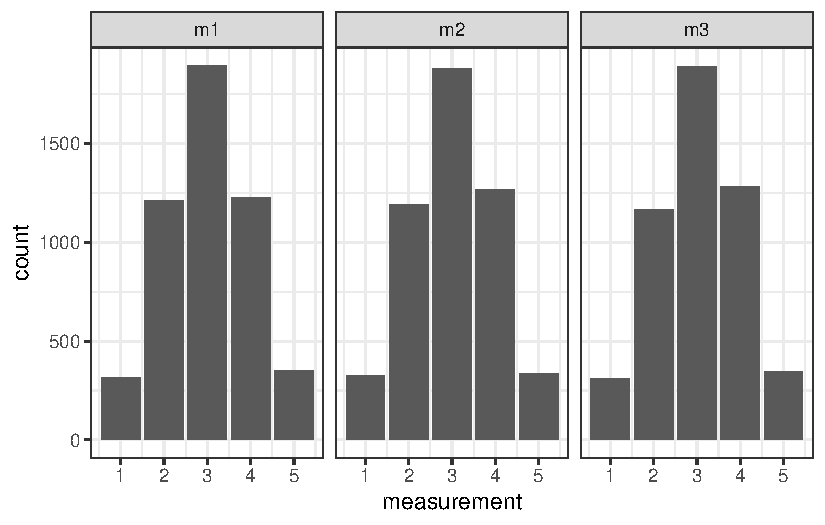
\includegraphics{./simulating-cfa-data_files/figure-pdf/unnamed-chunk-2-1.pdf}

}

\end{figure}

Unsurprisingly, the \texttt{lavaa::cfa()} function is able to recover
the cutpoints and the loadings:

\begin{Shaded}
\begin{Highlighting}[]
\CommentTok{\# Fit the model}
\NormalTok{fit\_1 }\OtherTok{\textless{}{-}} \FunctionTok{cfa}\NormalTok{(pop.model, }\AttributeTok{data =}\NormalTok{ fake\_dat, }\AttributeTok{ordered =} \FunctionTok{c}\NormalTok{(}\StringTok{"m1"}\NormalTok{, }\StringTok{"m2"}\NormalTok{, }\StringTok{"m3"}\NormalTok{))}

\NormalTok{tidy\_fit }\OtherTok{\textless{}{-}}\NormalTok{ fit\_1 }\SpecialCharTok{|\textgreater{}}\NormalTok{ broom}\SpecialCharTok{::}\FunctionTok{tidy}\NormalTok{()}

\CommentTok{\# Filter the data}
\NormalTok{filtered\_data }\OtherTok{\textless{}{-}}\NormalTok{ tidy\_fit }\SpecialCharTok{\%\textgreater{}\%} 
  \FunctionTok{filter}\NormalTok{(}\FunctionTok{grepl}\NormalTok{(}\StringTok{"f1 =\textasciitilde{}"}\NormalTok{, term) }\SpecialCharTok{|} \FunctionTok{grepl}\NormalTok{(}\StringTok{"}\SpecialCharTok{\textbackslash{}\textbackslash{}}\StringTok{|"}\NormalTok{, term)) }\SpecialCharTok{\%\textgreater{}\%} 
  \FunctionTok{select}\NormalTok{(term, estimate)}

\CommentTok{\# Create the table}
\NormalTok{filtered\_data }\SpecialCharTok{\%\textgreater{}\%}
  \FunctionTok{gt}\NormalTok{() }\SpecialCharTok{\%\textgreater{}\%}
  \FunctionTok{tab\_header}\NormalTok{(}
    \AttributeTok{title =} \StringTok{"Loadings and Cutpoints"}
\NormalTok{  ) }\SpecialCharTok{\%\textgreater{}\%}
  \FunctionTok{cols\_label}\NormalTok{(}
    \AttributeTok{term =} \StringTok{"Parameter"}\NormalTok{,}
    \AttributeTok{estimate =} \StringTok{"Estimate"}
\NormalTok{  ) }\SpecialCharTok{\%\textgreater{}\%}
  \FunctionTok{fmt\_number}\NormalTok{(}
    \AttributeTok{columns =} \FunctionTok{c}\NormalTok{(estimate),}
    \AttributeTok{decimals =} \DecValTok{2}
\NormalTok{  )}
\end{Highlighting}
\end{Shaded}

\begin{longtable}{lr}
\caption*{
{\large Loadings and Cutpoints}
} \\ 
\toprule
Parameter & Estimate \\ 
\midrule
f1 =\textasciitilde{} m1 & $0.80$ \\ 
f1 =\textasciitilde{} m2 & $0.80$ \\ 
f1 =\textasciitilde{} m3 & $0.80$ \\ 
m1 | t1 & $-1.50$ \\ 
m1 | t2 & $-0.50$ \\ 
m1 | t3 & $0.50$ \\ 
m1 | t4 & $1.50$ \\ 
m2 | t1 & $-1.50$ \\ 
m2 | t2 & $-0.50$ \\ 
m2 | t3 & $0.50$ \\ 
m2 | t4 & $1.50$ \\ 
m3 | t1 & $-1.50$ \\ 
m3 | t2 & $-0.50$ \\ 
m3 | t3 & $0.50$ \\ 
m3 | t4 & $1.50$ \\ 
\bottomrule
\end{longtable}

But what if we want the measured variables to take on some other shape?
We can just follow the same approach, slicing up the space beneath the
standard normal distribution to allocate probability mass however we
like. For example, say we want the categories to follow a uniform
distribution we can set the cutpoints at the distribution's quintiles,
so that each has equal probability mass. Let's figure out what those
are:

\begin{Shaded}
\begin{Highlighting}[]
\FunctionTok{qnorm}\NormalTok{(}\FunctionTok{c}\NormalTok{(}\FloatTok{0.2}\NormalTok{, }\FloatTok{0.4}\NormalTok{, }\FloatTok{0.6}\NormalTok{, }\FloatTok{0.8}\NormalTok{))}
\end{Highlighting}
\end{Shaded}

\begin{verbatim}
[1] -0.8416212 -0.2533471  0.2533471  0.8416212
\end{verbatim}

Great. Now let's plug them into the model.

\begin{Shaded}
\begin{Highlighting}[]
\NormalTok{pop.model }\OtherTok{\textless{}{-}} \StringTok{\textquotesingle{} }
\StringTok{  f1 =\textasciitilde{} .8*m1 + .8*m2 + .8*m3}

\StringTok{  m1 | {-}0.8416212*t1 + {-}0.2533471*t2 + 0.2533471*t3 + 0.8416212*t4}
\StringTok{  m2 | {-}0.8416212*t1 + {-}0.2533471*t2 + 0.2533471*t3 + 0.8416212*t4}
\StringTok{  m3 | {-}0.8416212*t1 + {-}0.2533471*t2 + 0.2533471*t3 + 0.8416212*t4}
\StringTok{\textquotesingle{}}

\CommentTok{\# Simulate data from the model}
\NormalTok{fake\_dat }\OtherTok{\textless{}{-}}\NormalTok{ lavaan}\SpecialCharTok{::}\FunctionTok{simulateData}\NormalTok{(}\AttributeTok{model =}\NormalTok{ pop.model, }\AttributeTok{sample.nobs =} \DecValTok{5000}\NormalTok{)}

\CommentTok{\# Visualize the measured dat}
\NormalTok{fake\_dat }\SpecialCharTok{|\textgreater{}}

  \FunctionTok{select}\NormalTok{(m1, m2, m3) }\SpecialCharTok{|\textgreater{}} 
  
  \FunctionTok{pivot\_longer}\NormalTok{(}\FunctionTok{everything}\NormalTok{(), }\AttributeTok{names\_to =} \StringTok{"var"}\NormalTok{, }\AttributeTok{values\_to =} \StringTok{"measurement"}\NormalTok{) }\SpecialCharTok{|\textgreater{}}

  \FunctionTok{ggplot}\NormalTok{() }\SpecialCharTok{+}
  \FunctionTok{geom\_bar}\NormalTok{(}\FunctionTok{aes}\NormalTok{(}\AttributeTok{x =}\NormalTok{ measurement)) }\SpecialCharTok{+}
  \FunctionTok{facet\_wrap}\NormalTok{(}\SpecialCharTok{\textasciitilde{}}\NormalTok{var) }\SpecialCharTok{+}
  \FunctionTok{theme\_bw}\NormalTok{()}
\end{Highlighting}
\end{Shaded}

\begin{figure}[H]

{\centering 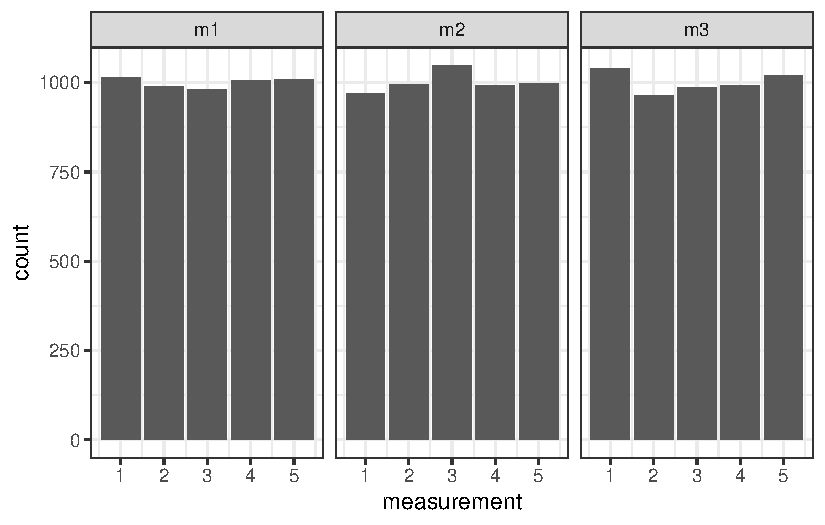
\includegraphics{./simulating-cfa-data_files/figure-pdf/unnamed-chunk-5-1.pdf}

}

\end{figure}

\hypertarget{bayesian-cfa}{%
\chapter{Bayesian CFA}\label{bayesian-cfa}}

\begin{Shaded}
\begin{Highlighting}[]
\FunctionTok{library}\NormalTok{(tidyverse)}
\FunctionTok{library}\NormalTok{(lavaan)}
\FunctionTok{library}\NormalTok{(blavaan)}
\FunctionTok{library}\NormalTok{(brms)}
\FunctionTok{library}\NormalTok{(tidybayes)}
\FunctionTok{library}\NormalTok{(survival)}
\FunctionTok{library}\NormalTok{(survminer)}

\FunctionTok{options}\NormalTok{(}\AttributeTok{brms.backend =} \StringTok{"cmdstanr"}\NormalTok{)}
\FunctionTok{options}\NormalTok{(}\AttributeTok{mc.cores =}\NormalTok{ parallel}\SpecialCharTok{::}\FunctionTok{detectCores}\NormalTok{())}
\end{Highlighting}
\end{Shaded}

\hypertarget{summary}{%
\section*{Summary}\label{summary}}
\addcontentsline{toc}{section}{Summary}

I recently did an analysis for a client who designs workforce skills
training programs. The client was interested in the relationship between
several latent skills for which they had collected measurements, and
time-to-employment following a skills training program. This document
presents the Bayesian workflow I used for that analysis, which involved
simultaneously estimating a factor model for the latent variables and
including them as regressors in a time-to-event analysis. Along the way
I show various approaches to simulating latent variable and
time-to-event data for model validation, and demonstrate the advantages
of the Bayesian approach to including latent regressors in a statistical
model, compared to traditional two-stage approaches involving factor
score point estimates.

\hypertarget{introduction}{%
\section{Introduction}\label{introduction}}

In the previous sections we've explored various aspects of the
traditional workflow for Confirmatory Factor Analysis, including the
basic model structure, the concepts of validity and reliability, classic
model goodness of fit tests, tests for measurement invariance, and
experimenting with custom error covariance structures. These are all
helpful tools for specifying quantitative theories about imaginary
constructs, and testing those theories with data.

But often you'll want to do more than just convince me the data are
consistent with \textbf{?@sec-intro}: you'll also have some theories
about how those imagined constructs relate to other measurements or
latent constructs. This opens the door to \textbf{Structural Equation
Modelling (SEM)}, which is a framework for simultaneously arguing that
my data are consistent with the imaginary constructs I have in mind,
\emph{and} that my data are consistent with the idea that those
constructs relate to each other according to a specific causal
structure.

In later chapters I'll be adding notes on the traditional SEM workflow.
But as a first step towards full SEM it is interesting to explore a more
basic situation where we only have latent \emph{predictors}, and want to
estimate the relationship between those latent predictors and an
\emph{observed outcome}, as opposed to a latent outcome with its own
measurement model. A traditional way of incorporating a CFA measurement
model into a fuller regression analysis for a measured dependent
variable proceeds in two steps:

\begin{enumerate}
\def\labelenumi{\arabic{enumi}.}
\tightlist
\item
  Fit the CFA model;
\item
  Generate factor scores for each observation;
\item
  Use those factor scores as predictors in a regression.
\end{enumerate}

For example, this is the approach taken by Kankaraš, Feron, and
Renbarger (2019) in their study of the relationship between latent
social/emotional skills and life outcomes such as academic achievement;
they use point-estimate factor scores for the latent variables as
predictors in the subsequent regressions on life outcome data. In some
cases they even do this iteratively, fitting measurement models on
point-estimate factor scores from measurement models fit on
point-estimate factor scores, and using \emph{those} point-estimates as
regression predictors! This approach is unsatisfactory because factor
scores are a function of the CFA model's parameter estimates, about
which there is uncertainty. If we only give our substantive regression
model a point-estimate factor score from the CFA model, we ignore this
uncertainty.

A better option is to fit a Bayesian model that fits the measurement
model and the substantive regression model simultaneously, so that the
model can incorporate its uncertainty from the CFA model into its
substantive parameter estimates and predictions. As we'll see below,
this approach is essentially just a Bayesian missing data analysis,
where the factor scores for each observation are treated as missing data
for which the model estimates a unique observation-specific parameter,
along with its own unique posterior distribution.

\hypertarget{the-plan}{%
\section{The Plan}\label{the-plan}}

In this document I'll demonstrate how to implement this Bayesian
approach with Stan. We'll iterate on this model a few times, gradually
incorporating concepts from previous chapters such as MTMM factor
analysis. At each stage we'll stick the following invented scenario: our
client has designed scales for the latent skills ``adaptability'' and
``collaboration'', and wants to test the validity of those scales and
estimate their relationship with time-to-employment for their program
graduates.

At each stage of the analysis we'll simulate a new dataset reflecting
our updated model, and show that the model can recover the true
simulation parameter estimates. We'll proceed as follows:

\begin{enumerate}
\def\labelenumi{\arabic{enumi}.}
\tightlist
\item
  Fit a simple Bayesian CFA with one factor and a basic measurement
  error covariance structure. We use the brms package to illustrate how
  Bayesian factor analysis is the same as Bayesian missing data
  analysis, but where \emph{all} of your observations are missing;
\item
  Fit a Bayesian CFA with two correlated factors. The brms package can't
  yet handle custom covariance structures for latent factors, so we
  swtich to raw Stan;
\item
  Update the model to include a custom error covariance structure à la
  MTMM;
\item
  Combine the MTMM model from the previous step with a parametric
  proportional hazards regression model;
\item
  Expand the model to include multilevel structure, with correlated
  varying effects for the regression predictors.
\end{enumerate}

I assume basic knowledge of R, Stan, and survial analysis.

\hypertarget{simple-bayesian-cfa-with-brms}{%
\section{Simple Bayesian CFA with
brms}\label{simple-bayesian-cfa-with-brms}}

Before diving into a full model with our two factors for
``adaptability'' and ``collabortion'' in raw Stan, in this section we'll
see how to fit a simple Bayesian CFA model in brms. Nothing fancy, just
one factor with 6 measurements. Here's the full model definition:

\[
\begin{aligned}
\begin{bmatrix}
m_{1} \\
m_{2} \\
m_{3} \\
m_{4} \\
m_{5} \\
m_{6}
\end{bmatrix}
&\sim \text{MVNormal}
\left(
\begin{bmatrix}
\mu_{m1} \\
\mu_{m2} \\
\mu_{m3} \\
\mu_{m4} \\
\mu_{m5} \\
\mu_{m6}
\end{bmatrix},
\Sigma_m
\right) \\
\\
\mu_{m1} &= \lambda_1 \text{f}_1, \quad \mu_{m2} = \lambda_2 \text{f}_1, \quad \mu_{m3} = \lambda_3 \text{f}_1 \\
\mu_{m4} &= \lambda_4 \text{f}_1, \quad \mu_{m5} = \lambda_5 \text{f}_1, \quad \mu_{m6} = \lambda_6 \text{f}_1 \\
\\
\text{f} &\sim \text{Normal}(\mu_\text{f}, \sigma_\text{f}^2) \\
\\
\Sigma_m &=
\begin{bmatrix}
\sigma_{m1}^2 & 0 & 0 & 0 & 0 & 0 \\
0 & \sigma_{m2}^2 & 0 & 0 & 0 & 0 \\
0 & 0 & \sigma_{m3}^2 & 0 & 0 & 0 \\
0 & 0 & 0 & \sigma_{m4}^2 & 0 & 0 \\
0 & 0 & 0 & 0 & \sigma_{m5}^2 & 0 \\
0 & 0 & 0 & 0 & 0 & \sigma_{m6}^2
\end{bmatrix}
\end{aligned}
\]

First we can simulate some data with the given factor structure using
the lavaan package's handy \texttt{simulateData()} function:

\begin{Shaded}
\begin{Highlighting}[]
\CommentTok{\# Specify the factor structure in classic lavaan syntax}
\NormalTok{basic.model }\OtherTok{\textless{}{-}} \StringTok{\textquotesingle{} }
\StringTok{  f1 =\textasciitilde{} .8*m1 + .1*m2 + .6*m3 + .2*m4 + .9*m5 + {-}.4*m6}
\StringTok{\textquotesingle{}}

\CommentTok{\# Simulate data from the specified model }
\NormalTok{fake\_dat }\OtherTok{\textless{}{-}}\NormalTok{ lavaan}\SpecialCharTok{::}\FunctionTok{simulateData}\NormalTok{(}\AttributeTok{model =}\NormalTok{ basic.model, }\AttributeTok{sample.nobs =} \DecValTok{4000}\NormalTok{)}
\end{Highlighting}
\end{Shaded}

We can take a peak at the resulting dataset to make sure everything
looks kosher. Looks like some simple normal densities, as expected:

\begin{Shaded}
\begin{Highlighting}[]
\CommentTok{\# Visualize the measured data}
\NormalTok{fake\_dat }\SpecialCharTok{|\textgreater{}}

  \FunctionTok{select}\NormalTok{(m1, m2, m3, m4, m5, m6) }\SpecialCharTok{|\textgreater{}}
  
  \FunctionTok{pivot\_longer}\NormalTok{(}\FunctionTok{everything}\NormalTok{(), }\AttributeTok{names\_to =} \StringTok{"var"}\NormalTok{, }\AttributeTok{values\_to =} \StringTok{"measurement"}\NormalTok{) }\SpecialCharTok{|\textgreater{}}

  \FunctionTok{ggplot}\NormalTok{() }\SpecialCharTok{+}
  \FunctionTok{geom\_density}\NormalTok{(}\FunctionTok{aes}\NormalTok{(}\AttributeTok{x =}\NormalTok{ measurement), }\AttributeTok{fill =} \StringTok{"mediumorchid"}\NormalTok{) }\SpecialCharTok{+}
  \FunctionTok{facet\_wrap}\NormalTok{(}\SpecialCharTok{\textasciitilde{}}\NormalTok{var) }\SpecialCharTok{+}
  \FunctionTok{theme\_minimal}\NormalTok{() }\SpecialCharTok{+}
  \FunctionTok{theme}\NormalTok{(}
    \AttributeTok{panel.grid.major =} \FunctionTok{element\_blank}\NormalTok{(),}
    \AttributeTok{panel.grid.minor =} \FunctionTok{element\_blank}\NormalTok{()}
\NormalTok{  )}
\end{Highlighting}
\end{Shaded}

\begin{figure}[H]

{\centering 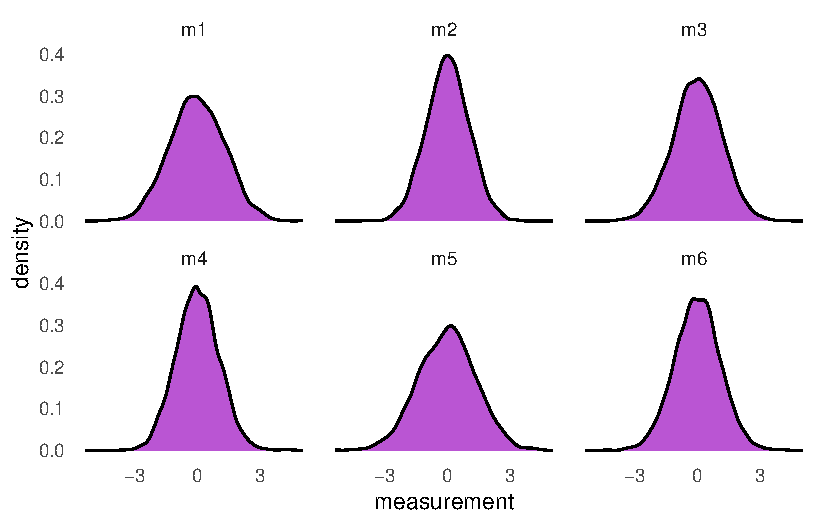
\includegraphics{./bayesian-cfa_files/figure-pdf/unnamed-chunk-3-1.pdf}

}

\end{figure}

Now we can specify a Bayesian model in brms that recovers the simulation
parameter values. I've worked from
\href{https://discourse.mc-stan.org/t/confirmatory-factor-analysis-using-brms/23139}{the
approach shared by Jack Bailey in a post on the Stan forum}. I like this
approach because it gives a nice conceptual perspective on what we're
actually doing when we're doing latant variable modelling: we're just
fitting a linear regression where the measured variables are all drawn
from a shared multivariate normal distribution, and where the linear
model components of their location parameters include a covariate for
which we \emph{only} have missing data. So the first thing we need to do
is add a column of all missing data for each of the latent variables.
Then we define the model with the same approach to identifiability
constraints that lavaan imposes by default, I.E. constraining the first
loading to be constant. The jargon term for this approach to ensuring
identifiability is the `marker variable approach':

\begin{Shaded}
\begin{Highlighting}[]
\CommentTok{\# Add the latent variable to the dataset as an all NA column}
\NormalTok{fake\_dat}\SpecialCharTok{$}\NormalTok{f1 }\OtherTok{\textless{}{-}} \ConstantTok{NA\_real\_}

\CommentTok{\# Define the model, with the coefficient for m1 fied to a constant for identifiability}
\NormalTok{bfit}\FloatTok{.1} \OtherTok{\textless{}{-}} \FunctionTok{brm}\NormalTok{(}
  \AttributeTok{formula =}
    \FunctionTok{bf}\NormalTok{(m1 }\SpecialCharTok{\textasciitilde{}} \DecValTok{0} \SpecialCharTok{+} \FunctionTok{mi}\NormalTok{(f1)) }\SpecialCharTok{+}
    \FunctionTok{bf}\NormalTok{(m2 }\SpecialCharTok{\textasciitilde{}} \DecValTok{0} \SpecialCharTok{+} \FunctionTok{mi}\NormalTok{(f1)) }\SpecialCharTok{+}
    \FunctionTok{bf}\NormalTok{(m3 }\SpecialCharTok{\textasciitilde{}} \DecValTok{0} \SpecialCharTok{+} \FunctionTok{mi}\NormalTok{(f1)) }\SpecialCharTok{+}
    \FunctionTok{bf}\NormalTok{(m4 }\SpecialCharTok{\textasciitilde{}} \DecValTok{0} \SpecialCharTok{+} \FunctionTok{mi}\NormalTok{(f1)) }\SpecialCharTok{+}
    \FunctionTok{bf}\NormalTok{(m5 }\SpecialCharTok{\textasciitilde{}} \DecValTok{0} \SpecialCharTok{+} \FunctionTok{mi}\NormalTok{(f1)) }\SpecialCharTok{+}
    \FunctionTok{bf}\NormalTok{(m6 }\SpecialCharTok{\textasciitilde{}} \DecValTok{0} \SpecialCharTok{+} \FunctionTok{mi}\NormalTok{(f1)) }\SpecialCharTok{+}
    \FunctionTok{bf}\NormalTok{(f1}\SpecialCharTok{|} \FunctionTok{mi}\NormalTok{() }\SpecialCharTok{\textasciitilde{}} \DecValTok{1}\NormalTok{) }\SpecialCharTok{+} 
    \FunctionTok{set\_rescor}\NormalTok{(}\AttributeTok{rescor =} \ConstantTok{FALSE}\NormalTok{),}
  \AttributeTok{family =} \FunctionTok{gaussian}\NormalTok{(),}
  \AttributeTok{prior =}
    \FunctionTok{prior}\NormalTok{(}\FunctionTok{constant}\NormalTok{(}\DecValTok{1}\NormalTok{), }\AttributeTok{class =} \StringTok{"b"}\NormalTok{, }\AttributeTok{resp =} \StringTok{"m1"}\NormalTok{) }\SpecialCharTok{+} \DocumentationTok{\#\# First loading fixed at 1, per the \textquotesingle{}marker variable\textquotesingle{} approach. }
    \FunctionTok{prior}\NormalTok{(}\FunctionTok{constant}\NormalTok{(}\DecValTok{1}\NormalTok{), }\AttributeTok{class =} \StringTok{"sigma"}\NormalTok{, }\AttributeTok{resp =} \StringTok{"m1"}\NormalTok{) }\SpecialCharTok{+}
    \FunctionTok{prior}\NormalTok{(}\FunctionTok{normal}\NormalTok{(}\DecValTok{0}\NormalTok{, }\DecValTok{10}\NormalTok{), }\AttributeTok{class =} \StringTok{"b"}\NormalTok{, }\AttributeTok{resp =} \StringTok{"m2"}\NormalTok{) }\SpecialCharTok{+}
    \FunctionTok{prior}\NormalTok{(}\FunctionTok{constant}\NormalTok{(}\DecValTok{1}\NormalTok{), }\AttributeTok{class =} \StringTok{"sigma"}\NormalTok{, }\AttributeTok{resp =} \StringTok{"m2"}\NormalTok{) }\SpecialCharTok{+}
    \FunctionTok{prior}\NormalTok{(}\FunctionTok{normal}\NormalTok{(}\DecValTok{0}\NormalTok{, }\DecValTok{10}\NormalTok{), }\AttributeTok{class =} \StringTok{"b"}\NormalTok{, }\AttributeTok{resp =} \StringTok{"m3"}\NormalTok{) }\SpecialCharTok{+}
    \FunctionTok{prior}\NormalTok{(}\FunctionTok{constant}\NormalTok{(}\DecValTok{1}\NormalTok{), }\AttributeTok{class =} \StringTok{"sigma"}\NormalTok{, }\AttributeTok{resp =} \StringTok{"m3"}\NormalTok{) }\SpecialCharTok{+}
    \FunctionTok{prior}\NormalTok{(}\FunctionTok{normal}\NormalTok{(}\DecValTok{0}\NormalTok{, }\DecValTok{10}\NormalTok{), }\AttributeTok{class =} \StringTok{"b"}\NormalTok{, }\AttributeTok{resp =} \StringTok{"m4"}\NormalTok{) }\SpecialCharTok{+}
    \FunctionTok{prior}\NormalTok{(}\FunctionTok{constant}\NormalTok{(}\DecValTok{1}\NormalTok{), }\AttributeTok{class =} \StringTok{"sigma"}\NormalTok{, }\AttributeTok{resp =} \StringTok{"m4"}\NormalTok{) }\SpecialCharTok{+}
    \FunctionTok{prior}\NormalTok{(}\FunctionTok{normal}\NormalTok{(}\DecValTok{0}\NormalTok{, }\DecValTok{10}\NormalTok{), }\AttributeTok{class =} \StringTok{"b"}\NormalTok{, }\AttributeTok{resp =} \StringTok{"m5"}\NormalTok{) }\SpecialCharTok{+}
    \FunctionTok{prior}\NormalTok{(}\FunctionTok{constant}\NormalTok{(}\DecValTok{1}\NormalTok{), }\AttributeTok{class =} \StringTok{"sigma"}\NormalTok{, }\AttributeTok{resp =} \StringTok{"m5"}\NormalTok{) }\SpecialCharTok{+}
    \FunctionTok{prior}\NormalTok{(}\FunctionTok{normal}\NormalTok{(}\DecValTok{0}\NormalTok{, }\DecValTok{10}\NormalTok{), }\AttributeTok{class =} \StringTok{"b"}\NormalTok{, }\AttributeTok{resp =} \StringTok{"m6"}\NormalTok{) }\SpecialCharTok{+}
    \FunctionTok{prior}\NormalTok{(}\FunctionTok{constant}\NormalTok{(}\DecValTok{1}\NormalTok{), }\AttributeTok{class =} \StringTok{"sigma"}\NormalTok{, }\AttributeTok{resp =} \StringTok{"m6"}\NormalTok{) }\SpecialCharTok{+}
    \FunctionTok{prior}\NormalTok{(}\FunctionTok{normal}\NormalTok{(}\DecValTok{0}\NormalTok{, }\DecValTok{10}\NormalTok{), }\AttributeTok{class =} \StringTok{"Intercept"}\NormalTok{, }\AttributeTok{resp =} \StringTok{"f1"}\NormalTok{) }\SpecialCharTok{+}
    \FunctionTok{prior}\NormalTok{(}\FunctionTok{cauchy}\NormalTok{(}\DecValTok{0}\NormalTok{, }\DecValTok{1}\NormalTok{), }\AttributeTok{class =} \StringTok{"sigma"}\NormalTok{, }\AttributeTok{resp =} \StringTok{"f1"}\NormalTok{),}
  \AttributeTok{data =}\NormalTok{ fake\_dat,}
  \AttributeTok{warmup =} \DecValTok{1000}\NormalTok{,}
  \AttributeTok{iter =} \DecValTok{6000}\NormalTok{,}
  \AttributeTok{file =} \StringTok{"fits/b07.01.rds"}
\NormalTok{)}
\end{Highlighting}
\end{Shaded}

A Bayesian missing data model treats each missing observation as a
parameter to estimate. And since the factor is 100\% missing data, this
means we end up with 4000 rows of data x 6000 samples x 4 chains =
96,000,000 MCMC samples for the factor scores alone, resulting in a
pretty big model file. This is too big for Github, so I'll only push the
draws we need to make sure the model recovered the true parameter
estimates.

First we can put the draws we need into a tidy format and do some
cleaning, then we can plot the draws to visualize the approximated
posteriors:

\begin{Shaded}
\begin{Highlighting}[]
\NormalTok{bfit.}\FloatTok{1.}\NormalTok{samples }\OtherTok{\textless{}{-}}\NormalTok{ bfit}\FloatTok{.1} \SpecialCharTok{|\textgreater{}}

  \CommentTok{\# Get the raw MCMC samples}
  \FunctionTok{gather\_draws}\NormalTok{(}
\NormalTok{    bsp\_m2\_mif1,}
\NormalTok{    bsp\_m3\_mif1,}
\NormalTok{    bsp\_m4\_mif1,}
\NormalTok{    bsp\_m5\_mif1,}
\NormalTok{    bsp\_m6\_mif1}
\NormalTok{  ) }\SpecialCharTok{|\textgreater{}}

  \CommentTok{\# Do some renaming for clarity}
  \FunctionTok{mutate}\NormalTok{(}\AttributeTok{.variable =} \FunctionTok{case\_when}\NormalTok{(}
\NormalTok{    .variable }\SpecialCharTok{==} \StringTok{"bsp\_m2\_mif1"} \SpecialCharTok{\textasciitilde{}} \StringTok{"Loading for m2"}\NormalTok{,}
\NormalTok{    .variable }\SpecialCharTok{==} \StringTok{"bsp\_m3\_mif1"} \SpecialCharTok{\textasciitilde{}} \StringTok{"Loading for m3"}\NormalTok{,}
\NormalTok{    .variable }\SpecialCharTok{==} \StringTok{"bsp\_m4\_mif1"} \SpecialCharTok{\textasciitilde{}} \StringTok{"Loading for m4"}\NormalTok{,}
\NormalTok{    .variable }\SpecialCharTok{==} \StringTok{"bsp\_m5\_mif1"} \SpecialCharTok{\textasciitilde{}} \StringTok{"Loading for m5"}\NormalTok{,}
\NormalTok{    .variable }\SpecialCharTok{==} \StringTok{"bsp\_m6\_mif1"} \SpecialCharTok{\textasciitilde{}} \StringTok{"Loading for m6"}
\NormalTok{  )) }\SpecialCharTok{|\textgreater{}} 

  \CommentTok{\# Add the true factor loadings from above}
  \FunctionTok{mutate}\NormalTok{(}\AttributeTok{true\_loading =} \FunctionTok{case\_when}\NormalTok{(}
\NormalTok{    .variable }\SpecialCharTok{==} \StringTok{"Loading for m2"} \SpecialCharTok{\textasciitilde{}}\NormalTok{ .}\DecValTok{1}\NormalTok{,}
\NormalTok{    .variable }\SpecialCharTok{==} \StringTok{"Loading for m3"} \SpecialCharTok{\textasciitilde{}}\NormalTok{ .}\DecValTok{6}\NormalTok{,}
\NormalTok{    .variable }\SpecialCharTok{==} \StringTok{"Loading for m4"} \SpecialCharTok{\textasciitilde{}}\NormalTok{ .}\DecValTok{2}\NormalTok{,}
\NormalTok{    .variable }\SpecialCharTok{==} \StringTok{"Loading for m5"} \SpecialCharTok{\textasciitilde{}}\NormalTok{ .}\DecValTok{9}\NormalTok{,}
\NormalTok{    .variable }\SpecialCharTok{==} \StringTok{"Loading for m6"} \SpecialCharTok{\textasciitilde{}} \SpecialCharTok{{-}}\NormalTok{.}\DecValTok{4}
\NormalTok{  )) }

\CommentTok{\# Save the tidy draws for reproducibility}
\FunctionTok{saveRDS}\NormalTok{(bfit.}\FloatTok{1.}\NormalTok{samples, }\StringTok{"fits/b07.01.samples.rds"}\NormalTok{)}
\end{Highlighting}
\end{Shaded}

\begin{Shaded}
\begin{Highlighting}[]
\CommentTok{\# Load the tidy samples}
\NormalTok{bfit.}\FloatTok{1.}\NormalTok{samples }\OtherTok{\textless{}{-}} \FunctionTok{readRDS}\NormalTok{(}\StringTok{"fits/b07.01.samples.rds"}\NormalTok{)}

\CommentTok{\# Plot}
\NormalTok{bfit.}\FloatTok{1.}\NormalTok{samples}\SpecialCharTok{|\textgreater{}}

  \FunctionTok{ggplot}\NormalTok{(}\FunctionTok{aes}\NormalTok{(}\AttributeTok{x =}\NormalTok{ .value, }\AttributeTok{fill =}\NormalTok{ .variable)) }\SpecialCharTok{+}
    \FunctionTok{stat\_halfeye}\NormalTok{(}\AttributeTok{fill =} \StringTok{"mediumorchid"}\NormalTok{) }\SpecialCharTok{+}
    \FunctionTok{geom\_vline}\NormalTok{(}\FunctionTok{aes}\NormalTok{(}\AttributeTok{xintercept =}\NormalTok{ true\_loading), }\AttributeTok{linetype =} \DecValTok{2}\NormalTok{) }\SpecialCharTok{+} 
    \FunctionTok{scale\_x\_continuous}\NormalTok{(}\AttributeTok{expand =} \FunctionTok{c}\NormalTok{(}\DecValTok{0}\NormalTok{, }\FloatTok{0.015}\NormalTok{)) }\SpecialCharTok{+}
    \FunctionTok{scale\_y\_continuous}\NormalTok{(}\AttributeTok{expand =} \FunctionTok{c}\NormalTok{(}\DecValTok{0}\NormalTok{, }\FloatTok{0.015}\NormalTok{)) }\SpecialCharTok{+}
    \FunctionTok{guides}\NormalTok{(}\AttributeTok{fill =} \StringTok{"none"}\NormalTok{) }\SpecialCharTok{+}
    \FunctionTok{labs}\NormalTok{(}\AttributeTok{x =} \StringTok{"lab"}\NormalTok{,}
       \AttributeTok{y =} \ConstantTok{NULL}\NormalTok{)  }\SpecialCharTok{+}
    \FunctionTok{facet\_wrap}\NormalTok{(}\SpecialCharTok{\textasciitilde{}}\NormalTok{.variable) }\SpecialCharTok{+}
    \FunctionTok{theme\_minimal}\NormalTok{() }\SpecialCharTok{+} 
    \FunctionTok{theme}\NormalTok{(}\AttributeTok{panel.grid.major =} \FunctionTok{element\_blank}\NormalTok{())}
\end{Highlighting}
\end{Shaded}

\begin{figure}[H]

{\centering 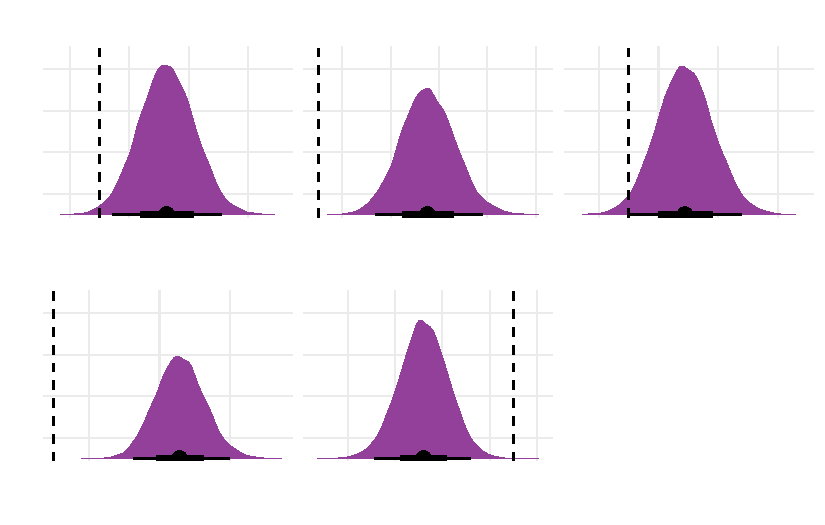
\includegraphics{./bayesian-cfa_files/figure-pdf/viz-draws-basic-1.pdf}

}

\end{figure}

In all cases the model is \emph{pretty close} to the true parameter
values, shown by the dashed lines. It's a bit worrying that the standard
errors are so small they fail to capture the true values, but this
illustrates the general proof of concept: we can do a pretty decent CFA
in brms.

In practice I would probably not choose brms for a simple CFA of this
kind, where we have no prior information to inform the parameter
estimates and no need to incorporate uncertainty in factor score
estimates into models of other variables. If I were committed to doing
this sort of model Bayesianly then I would use the amazing blavaan
package, which works with lavaan syntax, allows you to specify custom
priors, and is lightening-fast compared to the brms version implemented
above. But blavaan is limited in the types of models it can handle, and
cannot fit the type of time-to-event model we are heading towards here.
Stan offers greater flexibility.

\hypertarget{bayesian-cfa-with-correlated-factors}{%
\section{Bayesian CFA with Correlated
Factors}\label{bayesian-cfa-with-correlated-factors}}

Now let's introduce our two factors ``adaptability'' and
``collaboration'', and expand the model to assume these two latent
factors may be correlated. People traditionally use this type of model
to assess the discriminant validity of their factors, as we saw in
Chapter~\ref{sec-basic-workflow}. The only change from the model in the
previous section is that now we imagine the two factors to be drawn from
a shared bivariate normal distribution in which the diagonals are the
factor-specific residual variances and the off-diagonals are the
between-factor covariance, given as the product of their estimated
correlation \(\rho\) and the two factor-specific variances. Here's the
updated model definition, with the covariance terms highlighted:

\[
\begin{aligned}
\begin{bmatrix}
m_{1} \\
m_{2} \\
m_{3} \\
m_{4} \\
m_{5} \\
m_{6}
\end{bmatrix}
&\sim \text{MVNormal}
\left(
\begin{bmatrix}
\mu_{m1} \\
\mu_{m2} \\
\mu_{m3} \\
\mu_{m4} \\
\mu_{m5} \\
\mu_{m6}
\end{bmatrix},
\Sigma_m
\right) \\
\\
\mu_{m1} &= \lambda_1 \text{adapt}, \quad \mu_{m2} = \lambda_2 \text{adapt}, \quad \mu_{m3} = \lambda_3 \text{adapt} \\
\mu_{m4} &= \lambda_4 \text{collab}, \quad \mu_{m5} = \lambda_5 \text{collab}, \quad \mu_{m6} = \lambda_6 \text{collab} \\
\\
\begin{bmatrix}
\text{adapt}_{i} \\
\text{collab}_{i}
\end{bmatrix}
&\sim \text{MVNormal}
\left(
\begin{bmatrix}
\mu_\text{adapt} \\
\mu_\text{collab}
\end{bmatrix},
\Sigma_f
\right) \\
\\
\Sigma_f &=
\begin{bmatrix}
\sigma_\text{adapt}^2 & \color{orchid}{\rho \sigma_\text{adapt} \sigma_\text{collab}} \\
\color{orchid}{\rho \sigma_\text{adapt} \sigma_\text{collab}} & \sigma_\text{adapt}^2
\end{bmatrix}
\\
\Sigma_m &=
\begin{bmatrix}
\sigma_{m1}^2 & 0 & 0 & 0 & 0 & 0 \\
0 & \sigma_{m2}^2 & 0 & 0 & 0 & 0 \\
0 & 0 & \sigma_{m3}^2 & 0 & 0 & 0 \\
0 & 0 & 0 & \sigma_{m4}^2 & 0 & 0 \\
0 & 0 & 0 & 0 & \sigma_{m5}^2 & 0 \\
0 & 0 & 0 & 0 & 0 & \sigma_{m6}^2
\end{bmatrix}
\end{aligned}
\]

We can update the lavaan model structure from the previous section to
simulate new data with correlated factors. Note that in the lavaan
syntax \texttt{f1\ \textasciitilde{}\textasciitilde{}\ .4*f2} we are
specifying the \emph{covariance} between the factors, not the
correlation. But as we'll see later, the distinction doesn't matter in
this case.

\begin{Shaded}
\begin{Highlighting}[]
\CommentTok{\# Declare the new model with correlated factors}
\NormalTok{correlated.factors.model }\OtherTok{\textless{}{-}} \StringTok{\textquotesingle{} }
\StringTok{  f1 =\textasciitilde{} .8*m1 + .6*m2 + .9*m3}
\StringTok{  f2 =\textasciitilde{} .1*m4 + .2*m5 + {-}.4*m6}
\StringTok{  f1 \textasciitilde{}\textasciitilde{} .4*f2}
\StringTok{\textquotesingle{}}

\CommentTok{\# Simulate data from the model}
\NormalTok{fake\_dat }\OtherTok{\textless{}{-}}\NormalTok{ lavaan}\SpecialCharTok{::}\FunctionTok{simulateData}\NormalTok{(}\AttributeTok{model =}\NormalTok{ correlated.factors.model, }\AttributeTok{sample.nobs =} \DecValTok{4000}\NormalTok{)}
\end{Highlighting}
\end{Shaded}

Now to fit a model to the simulated data. We'll use raw Stan from now
on, because brms doesn't currently support setting constraints on
individual correlation terms in the model, even in the form of constant
priors. \href{https://github.com/paul-buerkner/brms/issues/957}{There
seems to be a plan} to include more SEM-like flexibility of covariance
matrixes in general in brms 3.0, but we do better to dive into raw Stan
anyway for added flexibility.

I tried a few different model definitions in Stan, but they all had
convergence issues and failed to recover the true parameter estimates.
Convergence in fitting a factor analysis can be tricky in general, and
things get even more complicated in a Bayesian context where we're using
MCMC to approximate the posterior. So I took to the Stan Forums, where I
found a few strategies for avoiding convergence issues when fitting this
kind of model. I have worked closely from the strategy provided in
\href{https://discourse.mc-stan.org/t/non-convergence-of-latent-variable-model/12450/13}{this
comment} by
\href{https://research.vu.nl/en/persons/mauricio-garnier-villarreal}{Mauricio
Garnier-Villarre}. Instead of the lavaan-default `marker variable
approach' to identifiability we used above in our brms model, Mauricio
fixes the factor means and variances at 0 and 1, respectively, which has
the benefit of letting the model freely estimate the \emph{all} of the
factor loadings. He also adds some code to sign-correct the estimated
loadings in the \texttt{generated\ quantities\{\}} block, which
apparently helps align estimates across chains. I just make a few minor
adjustments such as removing intercepts from the linear predictors of
the factors to better align the model with the lavaan defaults. Here is
the Stan code:

\begin{Shaded}
\begin{Highlighting}[]
\KeywordTok{data}\NormalTok{ \{}
  \DataTypeTok{int}\NormalTok{ N; }\CommentTok{// sample size}
  \DataTypeTok{int}\NormalTok{ P; }\CommentTok{// number of variables}
  \DataTypeTok{int}\NormalTok{ D; }\CommentTok{// number of factors}
  \DataTypeTok{array}\NormalTok{[N] }\DataTypeTok{vector}\NormalTok{[P] X; }\CommentTok{// data matrix of order [N,P]}
  \DataTypeTok{int}\NormalTok{ n\_lam; }\CommentTok{// how many factor loadings are estimated}
\NormalTok{\}}
\KeywordTok{parameters}\NormalTok{ \{}
  \DataTypeTok{matrix}\NormalTok{[N, D] FS\_UNC; }\CommentTok{// factor scores, matrix of order [N,D]}
  \DataTypeTok{cholesky\_factor\_corr}\NormalTok{[D] L\_corr\_d; }\CommentTok{// cholesky correlation between factors}
  \DataTypeTok{vector}\NormalTok{\textless{}}\KeywordTok{lower}\NormalTok{=}\DecValTok{0}\NormalTok{\textgreater{}[P] sd\_p; }\CommentTok{// residual sd for each variable}
  \DataTypeTok{vector}\NormalTok{\textless{}}\KeywordTok{lower}\NormalTok{={-}}\DecValTok{30}\NormalTok{, }\KeywordTok{upper}\NormalTok{=}\DecValTok{30}\NormalTok{\textgreater{}[n\_lam] lam\_UNC; }\CommentTok{// A bunch of lightly{-}constrained factor loadings}
\NormalTok{\}}
\KeywordTok{transformed parameters}\NormalTok{ \{}
  \CommentTok{// a vector to hold the factor means, which will be a bunch of 0s}
  \DataTypeTok{vector}\NormalTok{[D] M;}
\NormalTok{  M = rep\_vector(}\DecValTok{0}\NormalTok{, D);}
  
  \CommentTok{// a vector to hold the factor SDs, which will be a bunch of 1s. }
  \DataTypeTok{vector}\NormalTok{\textless{}}\KeywordTok{lower}\NormalTok{=}\DecValTok{0}\NormalTok{\textgreater{}[D] Sd\_d;}
\NormalTok{  Sd\_d = rep\_vector(}\DecValTok{1}\NormalTok{, D);}
  
  \CommentTok{// A vector to hold the linear predictors for the manifest variables, which are each a deterministic function of loading*factor\_score}
  \DataTypeTok{array}\NormalTok{[N] }\DataTypeTok{vector}\NormalTok{[P] mu\_UNC;}
  \ControlFlowTok{for}\NormalTok{ (i }\ControlFlowTok{in} \DecValTok{1}\NormalTok{ : N) \{}
\NormalTok{    mu\_UNC[i, }\DecValTok{1}\NormalTok{] = lam\_UNC[}\DecValTok{1}\NormalTok{] * FS\_UNC[i, }\DecValTok{1}\NormalTok{];}
\NormalTok{    mu\_UNC[i, }\DecValTok{2}\NormalTok{] = lam\_UNC[}\DecValTok{2}\NormalTok{] * FS\_UNC[i, }\DecValTok{1}\NormalTok{];}
\NormalTok{    mu\_UNC[i, }\DecValTok{3}\NormalTok{] = lam\_UNC[}\DecValTok{3}\NormalTok{] * FS\_UNC[i, }\DecValTok{1}\NormalTok{];}
\NormalTok{    mu\_UNC[i, }\DecValTok{4}\NormalTok{] = lam\_UNC[}\DecValTok{4}\NormalTok{] * FS\_UNC[i, }\DecValTok{2}\NormalTok{];}
\NormalTok{    mu\_UNC[i, }\DecValTok{5}\NormalTok{] = lam\_UNC[}\DecValTok{5}\NormalTok{] * FS\_UNC[i, }\DecValTok{2}\NormalTok{];}
\NormalTok{    mu\_UNC[i, }\DecValTok{6}\NormalTok{] = lam\_UNC[}\DecValTok{6}\NormalTok{] * FS\_UNC[i, }\DecValTok{2}\NormalTok{];}
\NormalTok{  \}}
  
  \CommentTok{// the var{-}covar matrix for the factors, a deterministic function of the deterministic SDs and the estimated rhos defined in parameters\{\}}
  \DataTypeTok{cholesky\_factor\_cov}\NormalTok{[D] L\_Sigma;}
\NormalTok{  L\_Sigma = diag\_pre\_multiply(Sd\_d, L\_corr\_d);}
\NormalTok{\}}
\KeywordTok{model}\NormalTok{ \{}
  \CommentTok{// Declare some priors}
\NormalTok{  L\_corr\_d \textasciitilde{} lkj\_corr\_cholesky(}\DecValTok{1}\NormalTok{); }\CommentTok{// Prior on factor corrs}
\NormalTok{  lam\_UNC \textasciitilde{} normal(}\DecValTok{0}\NormalTok{, }\DecValTok{10}\NormalTok{); }\CommentTok{// Prior on loadings}
\NormalTok{  sd\_p \textasciitilde{} cauchy(}\DecValTok{0}\NormalTok{, }\FloatTok{2.5}\NormalTok{); }\CommentTok{// Prior on residual SDs of manifest variables}
  
  \CommentTok{// Set up the likelihoods of the manifest and latent factors}
  \ControlFlowTok{for}\NormalTok{ (i }\ControlFlowTok{in} \DecValTok{1}\NormalTok{ : N) \{}
    \ControlFlowTok{for}\NormalTok{ (j }\ControlFlowTok{in} \DecValTok{1}\NormalTok{ : P) \{}
      \CommentTok{// Manifest variables}
\NormalTok{      X[i, j] \textasciitilde{} normal(mu\_UNC[i, j], sd\_p[j]);}
\NormalTok{    \}}
    \CommentTok{// Latent factors}
\NormalTok{    FS\_UNC[i] \textasciitilde{} multi\_normal\_cholesky(M, L\_Sigma);}
\NormalTok{  \}}
\NormalTok{\}}
\KeywordTok{generated quantities}\NormalTok{ \{}
  \DataTypeTok{corr\_matrix}\NormalTok{[D] Rho\_UNC; }\CommentTok{/// correlation matrix}
  \DataTypeTok{corr\_matrix}\NormalTok{[D] Rho; }\CommentTok{/// correlation matrix}
  \DataTypeTok{matrix}\NormalTok{[P, D] lam; }\CommentTok{// factor loadings}
  \DataTypeTok{matrix}\NormalTok{[N, D] FS; }\CommentTok{// factor scores, matrix of order [N,D]}
  
  \CommentTok{// Do some fancy things to sign{-}correct the parameter estimates.}
  \CommentTok{// The idea seems to be that when we estimate the loadings with unconstrained signs}
  \CommentTok{// It can lead to identification issues. So we take these steps to correct the signs.}
  \CommentTok{// See this Stan forum comment for more: https://discourse.mc{-}stan.org/t/non{-}convergence{-}of{-}latent{-}variable{-}model/12450/10?}
\NormalTok{  Rho\_UNC = multiply\_lower\_tri\_self\_transpose(L\_corr\_d);}
\NormalTok{  Rho = Rho\_UNC;}
\NormalTok{  FS = FS\_UNC;}
\NormalTok{  lam = rep\_matrix(}\DecValTok{0}\NormalTok{, P, D);}
\NormalTok{  lam[}\DecValTok{1}\NormalTok{ : }\DecValTok{3}\NormalTok{, }\DecValTok{1}\NormalTok{] = to\_vector(lam\_UNC[}\DecValTok{1}\NormalTok{ : }\DecValTok{3}\NormalTok{]);}
\NormalTok{  lam[}\DecValTok{4}\NormalTok{ : }\DecValTok{6}\NormalTok{, }\DecValTok{2}\NormalTok{] = to\_vector(lam\_UNC[}\DecValTok{4}\NormalTok{ : }\DecValTok{6}\NormalTok{]);}
  
  \CommentTok{// factor 1}
  \ControlFlowTok{if}\NormalTok{ (lam\_UNC[}\DecValTok{1}\NormalTok{] \textless{} }\DecValTok{0}\NormalTok{) \{}
\NormalTok{    lam[}\DecValTok{1}\NormalTok{ : }\DecValTok{3}\NormalTok{, }\DecValTok{1}\NormalTok{] = to\_vector({-}}\DecValTok{1}\NormalTok{ * lam\_UNC[}\DecValTok{1}\NormalTok{ : }\DecValTok{3}\NormalTok{]);}
\NormalTok{    FS[ : , }\DecValTok{1}\NormalTok{] = to\_vector({-}}\DecValTok{1}\NormalTok{ * FS\_UNC[ : , }\DecValTok{1}\NormalTok{]);}
    
    \ControlFlowTok{if}\NormalTok{ (lam\_UNC[}\DecValTok{4}\NormalTok{] \textgreater{} }\DecValTok{0}\NormalTok{) \{}
\NormalTok{      Rho[}\DecValTok{1}\NormalTok{, }\DecValTok{2}\NormalTok{] = {-}}\DecValTok{1}\NormalTok{ * Rho\_UNC[}\DecValTok{1}\NormalTok{, }\DecValTok{2}\NormalTok{];}
\NormalTok{      Rho[}\DecValTok{2}\NormalTok{, }\DecValTok{1}\NormalTok{] = {-}}\DecValTok{1}\NormalTok{ * Rho\_UNC[}\DecValTok{2}\NormalTok{, }\DecValTok{1}\NormalTok{];}
\NormalTok{    \}}
\NormalTok{  \}}
  \CommentTok{// factor 2}
  \ControlFlowTok{if}\NormalTok{ (lam\_UNC[}\DecValTok{4}\NormalTok{] \textless{} }\DecValTok{0}\NormalTok{) \{}
\NormalTok{    lam[}\DecValTok{4}\NormalTok{ : }\DecValTok{6}\NormalTok{, }\DecValTok{2}\NormalTok{] = to\_vector({-}}\DecValTok{1}\NormalTok{ * lam\_UNC[}\DecValTok{4}\NormalTok{ : }\DecValTok{6}\NormalTok{]);}
\NormalTok{    FS[ : , }\DecValTok{2}\NormalTok{] = to\_vector({-}}\DecValTok{1}\NormalTok{ * FS\_UNC[ : , }\DecValTok{2}\NormalTok{]);}
    
    \ControlFlowTok{if}\NormalTok{ (lam\_UNC[}\DecValTok{1}\NormalTok{] \textgreater{} }\DecValTok{0}\NormalTok{) \{}
\NormalTok{      Rho[}\DecValTok{2}\NormalTok{, }\DecValTok{1}\NormalTok{] = {-}}\DecValTok{1}\NormalTok{ * Rho\_UNC[}\DecValTok{2}\NormalTok{, }\DecValTok{1}\NormalTok{];}
\NormalTok{      Rho[}\DecValTok{1}\NormalTok{, }\DecValTok{2}\NormalTok{] = {-}}\DecValTok{1}\NormalTok{ * Rho\_UNC[}\DecValTok{1}\NormalTok{, }\DecValTok{2}\NormalTok{];}
\NormalTok{    \}}
\NormalTok{  \}}
\NormalTok{\}}
\end{Highlighting}
\end{Shaded}

Now we can compile and run the model:

\begin{Shaded}
\begin{Highlighting}[]
\CommentTok{\# Write the raw Stan code from an R string to a Stan file}
\NormalTok{stan\_file }\OtherTok{\textless{}{-}}\NormalTok{ cmdstanr}\SpecialCharTok{::}\FunctionTok{write\_stan\_file}\NormalTok{(stan\_model\_code)}

\CommentTok{\# Autoformat the model syntax to preempt any warnings at compile time}
\NormalTok{model }\OtherTok{\textless{}{-}}\NormalTok{ cmdstanr}\SpecialCharTok{::}\FunctionTok{cmdstan\_model}\NormalTok{(stan\_file, }\AttributeTok{compile =} \ConstantTok{FALSE}\NormalTok{)}
\NormalTok{model}\SpecialCharTok{$}\FunctionTok{format}\NormalTok{(}\AttributeTok{canonicalize =} \ConstantTok{TRUE}\NormalTok{)}

\CommentTok{\# Compile the model from the Stan file}
\NormalTok{model }\OtherTok{\textless{}{-}}\NormalTok{ cmdstanr}\SpecialCharTok{::}\FunctionTok{cmdstan\_model}\NormalTok{(stan\_file)}

\CommentTok{\# Put the data into a list format Stan can understand}
\NormalTok{X }\OtherTok{\textless{}{-}} \FunctionTok{as.matrix}\NormalTok{(fake\_dat)}
\NormalTok{P }\OtherTok{\textless{}{-}} \FunctionTok{ncol}\NormalTok{(fake\_dat) }
\NormalTok{N }\OtherTok{\textless{}{-}} \FunctionTok{nrow}\NormalTok{(fake\_dat)}
\NormalTok{D }\OtherTok{\textless{}{-}} \DecValTok{2}

\NormalTok{data\_list }\OtherTok{\textless{}{-}} \FunctionTok{list}\NormalTok{(}\AttributeTok{N=}\NormalTok{N,}\AttributeTok{P=}\NormalTok{P,}\AttributeTok{D=}\NormalTok{D,}\AttributeTok{X=}\NormalTok{X, }\AttributeTok{n\_lam=}\DecValTok{6}\NormalTok{)}

\CommentTok{\# Fit the model}
\NormalTok{fit }\OtherTok{\textless{}{-}}\NormalTok{ model}\SpecialCharTok{$}\FunctionTok{sample}\NormalTok{(}
  \AttributeTok{data =}\NormalTok{ data\_list,}
  \AttributeTok{seed =} \DecValTok{199}\NormalTok{,}
  \AttributeTok{chains =} \DecValTok{4}\NormalTok{,}
  \AttributeTok{parallel\_chains =} \DecValTok{4}\NormalTok{,}
  \AttributeTok{iter\_warmup =} \DecValTok{1000}\NormalTok{,}
  \AttributeTok{iter\_sampling =} \DecValTok{6000}\NormalTok{,}
  \AttributeTok{adapt\_delta=}\FloatTok{0.99}\NormalTok{, }
  \AttributeTok{max\_treedepth =} \DecValTok{12}\NormalTok{,}
  \AttributeTok{refresh =} \DecValTok{100} 
\NormalTok{)}

\CommentTok{\# Save the resulting model fit}
\FunctionTok{saveRDS}\NormalTok{(fit, }\StringTok{"fits/b07.02.rds"}\NormalTok{)}
\end{Highlighting}
\end{Shaded}

The model took about 5 hours to sample and the resulting .csv files
containing the MCMC samples are large -- on the order of 2.5GB each.
Fortunately we are able to selectively load only the draws from
variables we're interested in, so we have no problem working in memory.

\begin{Shaded}
\begin{Highlighting}[]
\CommentTok{\# Load the cmdstanr model object}
\NormalTok{fit }\OtherTok{\textless{}{-}} \FunctionTok{readRDS}\NormalTok{(}\StringTok{"fits/b07.02.rds"}\NormalTok{)}

\CommentTok{\# Load the MCMC draws from the variables we care about}
\NormalTok{draws }\OtherTok{\textless{}{-}}\NormalTok{ fit}\SpecialCharTok{$}\FunctionTok{draws}\NormalTok{(}
  \AttributeTok{variables =} \FunctionTok{c}\NormalTok{(}
  \StringTok{"lam[1,1]"}\NormalTok{,}
  \StringTok{"lam[2,1]"}\NormalTok{,}
  \StringTok{"lam[3,1]"}\NormalTok{,}
  \StringTok{"lam[4,2]"}\NormalTok{,}
  \StringTok{"lam[5,2]"}\NormalTok{,}
  \StringTok{"lam[6,2]"}\NormalTok{,}
  \StringTok{"Rho[2,1]"}
\NormalTok{  )}
\NormalTok{)}

\CommentTok{\# Save the result}
\FunctionTok{saveRDS}\NormalTok{(draws, }\StringTok{"fits/b07.02.samples.rds"}\NormalTok{)}
\end{Highlighting}
\end{Shaded}

Now we can explore the results. One important point is that we can
interpret the Stan model's estimates of the correlation coefficient
between the two factors directly as covariances (IE analogous to the
true parameter simulated with lavaan), because we fixed the factor
standard deviations to be equal to 1. Put differently, because our
sigmas are both equal to 1, this equation:

\$\$

\begin{aligned}
\rho(X, Y) = \frac{\text{Cov}(X, Y)}{\sigma_X \sigma_Y}
\end{aligned}

\$\$

Just becomes this: \$\$

\begin{aligned}
\rho(X, Y) = \frac{\text{Cov}(X, Y)}{1 * 1} = \text{Cov}(X, Y)
\end{aligned}

\$\$

We're interested in the loadings and the between-factor covariance. So
we can wrangle the MCMC samples for those variables and plot them to
look at the estimated posteriers. First let's look at the loadings.
Based on this plot it looks like the model did pretty well -- the
posterior peak is close to the true value for all of the loadings:

\begin{Shaded}
\begin{Highlighting}[]
\CommentTok{\# Load the draws for the loadings and correlation }
\NormalTok{draws }\OtherTok{\textless{}{-}} \FunctionTok{readRDS}\NormalTok{(}\StringTok{"fits/b07.02.samples.rds"}\NormalTok{)}

\CommentTok{\# Plot}
\NormalTok{dplt }\OtherTok{\textless{}{-}}\NormalTok{ draws }\SpecialCharTok{|\textgreater{}}

  \CommentTok{\# Get the raw draws for the factor loadings and the beween{-}factor correlation coefficient}
  \FunctionTok{gather\_draws}\NormalTok{(}
    \StringTok{\textasciigrave{}}\AttributeTok{lam[1,1]}\StringTok{\textasciigrave{}}\NormalTok{,}
    \StringTok{\textasciigrave{}}\AttributeTok{lam[2,1]}\StringTok{\textasciigrave{}}\NormalTok{,}
    \StringTok{\textasciigrave{}}\AttributeTok{lam[3,1]}\StringTok{\textasciigrave{}}\NormalTok{,}
    \StringTok{\textasciigrave{}}\AttributeTok{lam[4,2]}\StringTok{\textasciigrave{}}\NormalTok{,}
    \StringTok{\textasciigrave{}}\AttributeTok{lam[5,2]}\StringTok{\textasciigrave{}}\NormalTok{,}
    \StringTok{\textasciigrave{}}\AttributeTok{lam[6,2]}\StringTok{\textasciigrave{}}\NormalTok{,}
    \StringTok{\textasciigrave{}}\AttributeTok{Rho[2,1]}\StringTok{\textasciigrave{}}
\NormalTok{  ) }\SpecialCharTok{|\textgreater{}}

  \CommentTok{\# Do some renaming for clarity}
  \FunctionTok{mutate}\NormalTok{(}\AttributeTok{.variable =} \FunctionTok{case\_when}\NormalTok{(}
\NormalTok{    .variable }\SpecialCharTok{==} \StringTok{"lam[1,1]"} \SpecialCharTok{\textasciitilde{}} \StringTok{"Loading for m1"}\NormalTok{,}
\NormalTok{    .variable }\SpecialCharTok{==} \StringTok{"lam[2,1]"} \SpecialCharTok{\textasciitilde{}} \StringTok{"Loading for m2"}\NormalTok{,}
\NormalTok{    .variable }\SpecialCharTok{==} \StringTok{"lam[3,1]"} \SpecialCharTok{\textasciitilde{}} \StringTok{"Loading for m3"}\NormalTok{,}
\NormalTok{    .variable }\SpecialCharTok{==} \StringTok{"lam[4,2]"} \SpecialCharTok{\textasciitilde{}} \StringTok{"Loading for m4"}\NormalTok{,}
\NormalTok{    .variable }\SpecialCharTok{==} \StringTok{"lam[5,2]"} \SpecialCharTok{\textasciitilde{}} \StringTok{"Loading for m5"}\NormalTok{,}
\NormalTok{    .variable }\SpecialCharTok{==} \StringTok{"lam[6,2]"} \SpecialCharTok{\textasciitilde{}} \StringTok{"Loading for m6"}\NormalTok{,}
\NormalTok{    .variable }\SpecialCharTok{==} \StringTok{"Rho[2,1]"} \SpecialCharTok{\textasciitilde{}} \StringTok{"Covariance for f1 \textasciitilde{} f2"}\NormalTok{,}
\NormalTok{  )) }\SpecialCharTok{|\textgreater{}}

  \CommentTok{\# Add the true factor loadings for plotting}
  \FunctionTok{mutate}\NormalTok{(}\AttributeTok{true\_loading =} \FunctionTok{case\_when}\NormalTok{(}
\NormalTok{    .variable }\SpecialCharTok{==} \StringTok{"Loading for m1"} \SpecialCharTok{\textasciitilde{}}\NormalTok{ .}\DecValTok{8}\NormalTok{,}
\NormalTok{    .variable }\SpecialCharTok{==} \StringTok{"Loading for m2"} \SpecialCharTok{\textasciitilde{}}\NormalTok{ .}\DecValTok{6}\NormalTok{,}
\NormalTok{    .variable }\SpecialCharTok{==} \StringTok{"Loading for m3"} \SpecialCharTok{\textasciitilde{}}\NormalTok{ .}\DecValTok{9}\NormalTok{,}
\NormalTok{    .variable }\SpecialCharTok{==} \StringTok{"Loading for m4"} \SpecialCharTok{\textasciitilde{}}\NormalTok{ .}\DecValTok{1}\NormalTok{,}
\NormalTok{    .variable }\SpecialCharTok{==} \StringTok{"Loading for m5"} \SpecialCharTok{\textasciitilde{}}\NormalTok{ .}\DecValTok{2}\NormalTok{,}
\NormalTok{    .variable }\SpecialCharTok{==} \StringTok{"Loading for m6"} \SpecialCharTok{\textasciitilde{}} \SpecialCharTok{{-}}\NormalTok{.}\DecValTok{4}\NormalTok{,}
\NormalTok{    .variable }\SpecialCharTok{==} \StringTok{"Covariance for f1 \textasciitilde{} f2"} \SpecialCharTok{\textasciitilde{}}\NormalTok{ .}\DecValTok{4}
\NormalTok{  )) }

\NormalTok{dplt }\SpecialCharTok{|\textgreater{}}

  \FunctionTok{filter}\NormalTok{(.variable }\SpecialCharTok{!=} \StringTok{"Covariance for f1 \textasciitilde{} f2"}\NormalTok{) }\SpecialCharTok{|\textgreater{}}

  \FunctionTok{ggplot}\NormalTok{(}\FunctionTok{aes}\NormalTok{(}\AttributeTok{x =}\NormalTok{ .value, }\AttributeTok{fill =}\NormalTok{ .variable)) }\SpecialCharTok{+}
  \FunctionTok{stat\_halfeye}\NormalTok{(}\AttributeTok{fill =} \StringTok{"mediumorchid"}\NormalTok{) }\SpecialCharTok{+}
  \FunctionTok{geom\_vline}\NormalTok{(}\FunctionTok{aes}\NormalTok{(}\AttributeTok{xintercept =}\NormalTok{ true\_loading), }\AttributeTok{linetype =} \DecValTok{2}\NormalTok{) }\SpecialCharTok{+} 
  \FunctionTok{scale\_x\_continuous}\NormalTok{(}\AttributeTok{expand =} \FunctionTok{c}\NormalTok{(}\DecValTok{0}\NormalTok{, }\FloatTok{0.015}\NormalTok{)) }\SpecialCharTok{+}
  \FunctionTok{scale\_y\_continuous}\NormalTok{(}\AttributeTok{expand =} \FunctionTok{c}\NormalTok{(}\DecValTok{0}\NormalTok{, }\FloatTok{0.015}\NormalTok{)) }\SpecialCharTok{+}
  \FunctionTok{guides}\NormalTok{(}\AttributeTok{fill =} \StringTok{"none"}\NormalTok{) }\SpecialCharTok{+}
  \FunctionTok{labs}\NormalTok{(}\AttributeTok{x =} \StringTok{"lab"}\NormalTok{,}
     \AttributeTok{y =} \ConstantTok{NULL}\NormalTok{)  }\SpecialCharTok{+}
  \FunctionTok{facet\_wrap}\NormalTok{(}\SpecialCharTok{\textasciitilde{}}\NormalTok{.variable, }\AttributeTok{scales =} \StringTok{"free\_x"}\NormalTok{) }\SpecialCharTok{+}
  \FunctionTok{theme\_minimal}\NormalTok{() }\SpecialCharTok{+} 
  \FunctionTok{theme}\NormalTok{(}\AttributeTok{panel.grid.major =} \FunctionTok{element\_blank}\NormalTok{())}
\end{Highlighting}
\end{Shaded}

\begin{figure}[H]

{\centering 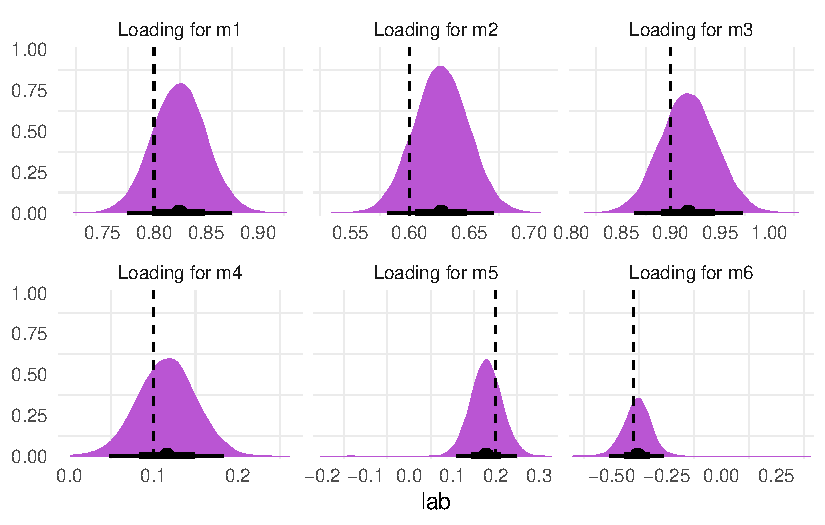
\includegraphics{./bayesian-cfa_files/figure-pdf/viz-loadings-2-fac-1.pdf}

}

\end{figure}

The model also seems to have accurately recovered the true
between-factor covariance, albeit with some unwholesome weirdness in the
tail of its approximated posterior. This weirdness appears to be pulling
the mean estimate upwards away from the true parameter estimate:

\begin{Shaded}
\begin{Highlighting}[]
\NormalTok{dplt }\SpecialCharTok{|\textgreater{}}

  \FunctionTok{filter}\NormalTok{(.variable }\SpecialCharTok{==} \StringTok{"Covariance for f1 \textasciitilde{} f2"}\NormalTok{) }\SpecialCharTok{|\textgreater{}}

  \FunctionTok{ggplot}\NormalTok{(}\FunctionTok{aes}\NormalTok{(}\AttributeTok{x =}\NormalTok{ .value, }\AttributeTok{fill =}\NormalTok{ .variable)) }\SpecialCharTok{+}
  \FunctionTok{stat\_halfeye}\NormalTok{(}\AttributeTok{fill =} \StringTok{"mediumorchid"}\NormalTok{) }\SpecialCharTok{+}
  \FunctionTok{geom\_vline}\NormalTok{(}\FunctionTok{aes}\NormalTok{(}\AttributeTok{xintercept =}\NormalTok{ true\_loading), }\AttributeTok{linetype =} \DecValTok{2}\NormalTok{) }\SpecialCharTok{+} 
  \FunctionTok{scale\_x\_continuous}\NormalTok{(}\AttributeTok{expand =} \FunctionTok{c}\NormalTok{(}\DecValTok{0}\NormalTok{, }\FloatTok{0.015}\NormalTok{)) }\SpecialCharTok{+}
  \FunctionTok{scale\_y\_continuous}\NormalTok{(}\AttributeTok{expand =} \FunctionTok{c}\NormalTok{(}\DecValTok{0}\NormalTok{, }\FloatTok{0.015}\NormalTok{)) }\SpecialCharTok{+}
  \FunctionTok{guides}\NormalTok{(}\AttributeTok{fill =} \StringTok{"none"}\NormalTok{) }\SpecialCharTok{+}
  \FunctionTok{labs}\NormalTok{(}\AttributeTok{x =} \StringTok{"lab"}\NormalTok{,}
     \AttributeTok{y =} \ConstantTok{NULL}\NormalTok{)  }\SpecialCharTok{+}
  \FunctionTok{facet\_wrap}\NormalTok{(}\SpecialCharTok{\textasciitilde{}}\NormalTok{.variable, }\AttributeTok{scales =} \StringTok{"free\_x"}\NormalTok{) }\SpecialCharTok{+}
  \FunctionTok{theme\_minimal}\NormalTok{() }\SpecialCharTok{+} 
  \FunctionTok{theme}\NormalTok{(}\AttributeTok{panel.grid.major =} \FunctionTok{element\_blank}\NormalTok{())}
\end{Highlighting}
\end{Shaded}

\begin{figure}[H]

{\centering 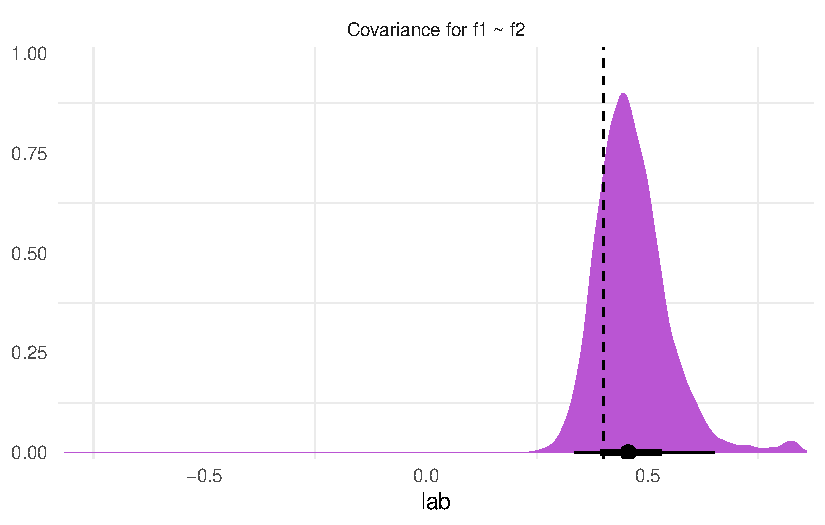
\includegraphics{./bayesian-cfa_files/figure-pdf/viz-cov-2-fac-1.pdf}

}

\end{figure}

We can also look at the MCMC convergence diagnostics such as rhat and
effective number of samples. Here we see that we have rhats slightly
greater than 1 for a few of the loadings and for rho. We also see that
loading 4, loading 6, and rho have a pretty low number of effective
samples. This is cause for concern, and in a real application I would
probably increase the number of MCMC iterations to see if we can improve
that effective sample size, and if that failed then I would think of
ways to reparameterize the model.

\begin{Shaded}
\begin{Highlighting}[]
\NormalTok{draws }\SpecialCharTok{|\textgreater{}} 

  \FunctionTok{summary}\NormalTok{() }\SpecialCharTok{|\textgreater{}}

  \FunctionTok{select}\NormalTok{(variable, rhat, ess\_bulk, ess\_tail) }\SpecialCharTok{|\textgreater{}}

  \FunctionTok{mutate}\NormalTok{(}\FunctionTok{across}\NormalTok{(}\FunctionTok{where}\NormalTok{(is.numeric), }\SpecialCharTok{\textasciitilde{}}\FunctionTok{round}\NormalTok{(.x, }\DecValTok{2}\NormalTok{))) }\SpecialCharTok{|\textgreater{}}

\NormalTok{  knitr}\SpecialCharTok{::}\FunctionTok{kable}\NormalTok{()}
\end{Highlighting}
\end{Shaded}

\begin{longtable}[]{@{}lrrr@{}}
\toprule()
variable & rhat & ess\_bulk & ess\_tail \\
\midrule()
\endhead
lam{[}1,1{]} & 1.00 & 8935.85 & 15354.16 \\
lam{[}2,1{]} & 1.00 & 16440.47 & 18512.91 \\
lam{[}3,1{]} & 1.00 & 6788.10 & 11132.78 \\
lam{[}4,2{]} & 1.01 & 806.68 & 450.49 \\
lam{[}5,2{]} & 1.00 & 1929.60 & 2266.63 \\
lam{[}6,2{]} & 1.02 & 345.23 & 122.68 \\
Rho{[}2,1{]} & 1.02 & 294.12 & 124.70 \\
\bottomrule()
\end{longtable}

The trace plots seem healthy overall, albeit with some occasional spikes
and some parts where one chain goes berzerk relative to the others.
Chain 4 for the between-factor correlation seems especially problematic,
with it following a strange trajectory during its final iterations.
Perhaps this explains why that variable has the highest rhat and
displays some irregularity in the tail of its approximated posterior.
Still, even for that parameter the chains seem generally healthy
overall.

\begin{Shaded}
\begin{Highlighting}[]
\CommentTok{\# Create a summary table}
\NormalTok{draws }\SpecialCharTok{|\textgreater{}}

\NormalTok{  bayesplot}\SpecialCharTok{::}\FunctionTok{mcmc\_trace}\NormalTok{() }\SpecialCharTok{+} 
  \FunctionTok{scale\_color\_manual}\NormalTok{(}\AttributeTok{values =} \FunctionTok{c}\NormalTok{(}\StringTok{"blue"}\NormalTok{, }\StringTok{"red"}\NormalTok{, }\StringTok{"orange"}\NormalTok{, }\StringTok{"mediumorchid"}\NormalTok{)) }\SpecialCharTok{+} 
  \FunctionTok{theme\_minimal}\NormalTok{() }\SpecialCharTok{+}
  \FunctionTok{theme}\NormalTok{(}
    \AttributeTok{panel.grid.major =} \FunctionTok{element\_blank}\NormalTok{(),}
    \AttributeTok{panel.grid.minor =} \FunctionTok{element\_blank}\NormalTok{()}
\NormalTok{  )}
\end{Highlighting}
\end{Shaded}

Overall we can feel ok about the model's performance here because it
recovered the true parameter values fairly well, but the MCMC
convergence checks suggest our chains were not totally happy.

One last thing before moving on: as mentioned above, we could have
simply used the blavaan package to fit this model instead of fussing
with custom Stan code. The blavaan version fits way faster and recovers
the true parameter estimates, but it is less flexible overall. And
again, crucially for the present analysis, there is no way to do
survival analysis with blavaan. But for posterity, below is the syntax
we would use to fit the model with blavaan. If we specify
\texttt{mcmcfile\ =\ TRUE} then the resulting Stan file gets written to
a new directory called \texttt{lavExport}, or we can supply a filepath
as the argument in which case the Stan file will get written there. The
file is very large (over 1000 lines) and confusing, I think because it
is precompiled to handle any possible model you could specify in R. The
Stan documentation includes
\href{https://mc-stan.org/users/documentation/case-studies/sem.html\#Confirmatory_Factor_Analysis_(CFA)}{an
example for specifying custom priors in a blavaan model}

\begin{Shaded}
\begin{Highlighting}[]
\CommentTok{\# Fit the model using the same lavaan{-}syntax model use used above to simulate the dataset}
\NormalTok{blavfit}\FloatTok{.1} \OtherTok{\textless{}{-}} \FunctionTok{bcfa}\NormalTok{(correlated.factors.model, }\AttributeTok{data=}\NormalTok{fake\_dat, }\AttributeTok{mcmcfile =}\NormalTok{ T)}

\CommentTok{\# Gaze at parameter estimates}
\NormalTok{blavfit}\FloatTok{.1} \SpecialCharTok{|\textgreater{}} \FunctionTok{summary}\NormalTok{()}

\CommentTok{\# Make sure the MCMC diagnostics are ok}
\FunctionTok{blavInspect}\NormalTok{(blavfit}\FloatTok{.1}\NormalTok{, }\StringTok{"mcobj"}\NormalTok{)}
\end{Highlighting}
\end{Shaded}

\hypertarget{bayesian-cfa-with-custom-covariance-structure}{%
\section{Bayesian CFA with Custom Covariance
Structure}\label{bayesian-cfa-with-custom-covariance-structure}}

In the previous section we moved beyond brms into raw Stan, which
allowed us to estimate the correlation between latent variables. But
often in latent variable modelling we also want to account for the
possibility that certain measured variables are confounded by some
shared unmeasured influences. One way to address this is to add another
factor to the model to account for these unmeasured influences, but it
can be simpler to just estimate a covariance term for those measured
variables. This is what Brown (2006) calls a `correlated uniqueness
model'. I have more detailed notes on these ideas in
Chapter~\ref{sec-mtmm}.

As an example of this scenario, we can imagine that the measured
variables m1 and m4 are confounded because they were both collected by
participant survey, while the other four measures were each collected by
different means. To reflect this change in the model, we need to change
the specification of the variance-covariance matrix of the shared
multivariable likelihood of the measured variables: where before all of
the off-diagonal elements were fixed at 0, now we need the off-diagonals
representing the covariance between m1 and m4 to be freely estimated.

Here's the updated model, with the new parameter highlighted in orange:

\[
\begin{aligned}
\begin{bmatrix}
m_{1} \\
m_{2} \\
m_{3} \\
m_{4} \\
m_{5} \\
m_{6}
\end{bmatrix}
&\sim \text{MVNormal}
\left(
\begin{bmatrix}
\mu_{m1} \\
\mu_{m2} \\
\mu_{m3} \\
\mu_{m4} \\
\mu_{m5} \\
\mu_{m6}
\end{bmatrix},
\Sigma_m
\right) \\
\\
\mu_{m1} &= \lambda_1 \text{adapt}, \quad \mu_{m2} = \lambda_2 \text{adapt}, \quad \mu_{m3} = \lambda_3 \text{adapt} \\
\mu_{m4} &= \lambda_4 \text{collab}, \quad \mu_{m5} = \lambda_5 \text{collab}, \quad \mu_{m6} = \lambda_6 \text{collab} \\
\\
\begin{bmatrix}
\text{adapt}_{i} \\
\text{collab}_{i}
\end{bmatrix}
&\sim \text{MVNormal}
\left(
\begin{bmatrix}
\mu_\text{adapt} \\
\mu_\text{collab}
\end{bmatrix},
\Sigma_f
\right) \\
\\
\Sigma_f &=
\begin{bmatrix}
\sigma_\text{adapt}^2 & \color{orchid}{\rho \sigma_\text{adapt} \sigma_\text{collab}} \\
\color{orchid}{\rho \sigma_\text{adapt} \sigma_\text{collab}} & \sigma_\text{adapt}^2
\end{bmatrix}
\\
\Sigma_m &=
\begin{bmatrix}
\sigma_{m1}^2 & 0 & 0 & \color{orange}{\rho\ \sigma_{m1} \sigma_{m4}} & 0 & 0 \\
0 & \sigma_{m2}^2 & 0 & 0 & 0 & 0 \\
0 & 0 & \sigma_{m3}^2 & 0 & 0 & 0 \\
\color{orange}{\rho \sigma_{m1} \sigma_{m4}} & 0 & 0 & \sigma_{m4}^2 & 0 & 0 \\
0 & 0 & 0 & 0 & \sigma_{m5}^2 & 0 \\
0 & 0 & 0 & 0 & 0 & \sigma_{m6}^2
\end{bmatrix}
\end{aligned}
\]

We can simulate data from this DAG using lavaan like we did for the two
models above, updating the syntax to give m1 and m4 a covariance of .4:

\begin{Shaded}
\begin{Highlighting}[]
\CommentTok{\# Declare the new lavaan model where m1 and m4 covary}
\NormalTok{mtmm.model }\OtherTok{\textless{}{-}} \StringTok{\textquotesingle{} }
\StringTok{  f1 =\textasciitilde{} .8*m1 + .6*m2 + .9*m3}
\StringTok{  f2 =\textasciitilde{} .1*m4 + .2*m5 + {-}.4*m6}
\StringTok{  f1 \textasciitilde{}\textasciitilde{} .4*f2}
\StringTok{  m1 \textasciitilde{}\textasciitilde{} .4*m4}
\StringTok{\textquotesingle{}}

\CommentTok{\# Simulate data from the lavaan model}
\NormalTok{fake\_dat }\OtherTok{\textless{}{-}}\NormalTok{ lavaan}\SpecialCharTok{::}\FunctionTok{simulateData}\NormalTok{(}\AttributeTok{model =}\NormalTok{ mtmm.model, }\AttributeTok{sample.nobs =} \DecValTok{4000}\NormalTok{)}
\end{Highlighting}
\end{Shaded}

We'll also need to add a new parameter to our Stan model to account for
the possibility that m1 and m4 covary. This only involves a few changes,
namely:

\begin{itemize}
\tightlist
\item
  \textbf{Parameters Block}: declare a matrix \texttt{L\_corr\_m1\_m4}
  to represent the Cholesky factorization of a correlation matrix
  between m1 and m4;
\item
  \textbf{Transformed Parameters Block}: declare the Cholesky
  factorization of a covariance matrix \texttt{L\_Sigma\_m1\_m4} and
  populate it by matrix-multiplying the standard deviations of m1 and m4
  with the Cholesky factorization of the correlation matrix declared
  above;
\item
  \textbf{Model Block}:, declare m1 and m4 as drawn from a shared
  bivariate normal distribution separate from the other measured
  variables. This is equivalent to declaring all measured variales as
  drawn from a shared distribution like in the mathematical rendering of
  the model shown above, but it is simpler to implement. We can use the
  Cholesky factorization of a multivariate normal distribution, with the
  vector of the mu estimates of m1 and m4 as the mean vector, and the
  Cholesky factorization of the covariance matrix
  \texttt{L\_Sigma\_m1\_m4} we declared above as the covariance matrix.
\item
  \textbf{Generated Quantities Block}: pull out the correlation
  parameter for m1 and m4 from the estimated variance covariance matrix
  so we can analyze it.
\end{itemize}

\begin{Shaded}
\begin{Highlighting}[]
\KeywordTok{data}\NormalTok{ \{}
  \DataTypeTok{int}\NormalTok{ N; }\CommentTok{// sample size}
  \DataTypeTok{int}\NormalTok{ P; }\CommentTok{// number of variables}
  \DataTypeTok{int}\NormalTok{ D; }\CommentTok{// number of factors}
  \DataTypeTok{array}\NormalTok{[N] }\DataTypeTok{vector}\NormalTok{[P] X; }\CommentTok{// data matrix of order [N,P]}
  \DataTypeTok{int}\NormalTok{ n\_lam; }\CommentTok{// how many factor loadings are estimated}
\NormalTok{\}}
\KeywordTok{parameters}\NormalTok{ \{}
  \DataTypeTok{matrix}\NormalTok{[N, D] FS\_UNC; }\CommentTok{// factor scores, matrix of order [N,D]}
  \DataTypeTok{cholesky\_factor\_corr}\NormalTok{[D] L\_corr\_d; }\CommentTok{// cholesky correlation between factors}
  \DataTypeTok{cholesky\_factor\_corr}\NormalTok{[}\DecValTok{2}\NormalTok{] L\_corr\_m1\_m4; }\CommentTok{// cholesky correlation between the m1 and m4}
  \DataTypeTok{vector}\NormalTok{\textless{}}\KeywordTok{lower}\NormalTok{=}\DecValTok{0}\NormalTok{\textgreater{}[P] sd\_p; }\CommentTok{// residual sd for each variable}
  \DataTypeTok{vector}\NormalTok{\textless{}}\KeywordTok{lower}\NormalTok{={-}}\DecValTok{30}\NormalTok{, }\KeywordTok{upper}\NormalTok{=}\DecValTok{30}\NormalTok{\textgreater{}[n\_lam] lam\_UNC; }\CommentTok{// A bunch of lightly{-}constrained factor loadings}
\NormalTok{\}}
\KeywordTok{transformed parameters}\NormalTok{ \{}
  \CommentTok{// a vector to hold the factor means, which will be a bunch of 0s}
  \DataTypeTok{vector}\NormalTok{[D] M;}
\NormalTok{  M = rep\_vector(}\DecValTok{0}\NormalTok{, D);}
  
  \CommentTok{// a vector to hold the factor SDs, which will be a bunch of 1s. }
  \DataTypeTok{vector}\NormalTok{\textless{}}\KeywordTok{lower}\NormalTok{=}\DecValTok{0}\NormalTok{\textgreater{}[D] Sd\_d;}
\NormalTok{  Sd\_d = rep\_vector(}\DecValTok{1}\NormalTok{, D);}
  
  \CommentTok{// A vector to hold the linear predictors for the manifest variables, which are each a deterministic function of loading*factor\_score}
  \DataTypeTok{array}\NormalTok{[N] }\DataTypeTok{vector}\NormalTok{[P] mu\_UNC;}
  \ControlFlowTok{for}\NormalTok{ (i }\ControlFlowTok{in} \DecValTok{1}\NormalTok{ : N) \{}
\NormalTok{    mu\_UNC[i, }\DecValTok{1}\NormalTok{] = lam\_UNC[}\DecValTok{1}\NormalTok{] * FS\_UNC[i, }\DecValTok{1}\NormalTok{];}
\NormalTok{    mu\_UNC[i, }\DecValTok{2}\NormalTok{] = lam\_UNC[}\DecValTok{2}\NormalTok{] * FS\_UNC[i, }\DecValTok{1}\NormalTok{];}
\NormalTok{    mu\_UNC[i, }\DecValTok{3}\NormalTok{] = lam\_UNC[}\DecValTok{3}\NormalTok{] * FS\_UNC[i, }\DecValTok{1}\NormalTok{];}
\NormalTok{    mu\_UNC[i, }\DecValTok{4}\NormalTok{] = lam\_UNC[}\DecValTok{4}\NormalTok{] * FS\_UNC[i, }\DecValTok{2}\NormalTok{];}
\NormalTok{    mu\_UNC[i, }\DecValTok{5}\NormalTok{] = lam\_UNC[}\DecValTok{5}\NormalTok{] * FS\_UNC[i, }\DecValTok{2}\NormalTok{];}
\NormalTok{    mu\_UNC[i, }\DecValTok{6}\NormalTok{] = lam\_UNC[}\DecValTok{6}\NormalTok{] * FS\_UNC[i, }\DecValTok{2}\NormalTok{];}
\NormalTok{  \}}
  
  \CommentTok{// the var{-}covar matrix for the factors, a deterministic function of the deterministic SDs and the estimated rhos defined in the parameters block}
  \DataTypeTok{cholesky\_factor\_cov}\NormalTok{[D] L\_Sigma;}
\NormalTok{  L\_Sigma = diag\_pre\_multiply(Sd\_d, L\_corr\_d);}

  \CommentTok{// Same, but for the var{-}covar matrix of m1 and m4}
  \DataTypeTok{cholesky\_factor\_cov}\NormalTok{[D] L\_Sigma\_m1\_m4;}
\NormalTok{  L\_Sigma\_m1\_m4 = diag\_pre\_multiply(sd\_p[\{}\DecValTok{1}\NormalTok{, }\DecValTok{4}\NormalTok{\}], L\_corr\_m1\_m4);}
\NormalTok{\}}
\KeywordTok{model}\NormalTok{ \{}
  \CommentTok{// Declare some priors}
\NormalTok{  L\_corr\_d \textasciitilde{} lkj\_corr\_cholesky(}\DecValTok{1}\NormalTok{); }\CommentTok{// Prior on factor corrs}
\NormalTok{  L\_corr\_m1\_m4 \textasciitilde{} lkj\_corr\_cholesky(}\DecValTok{1}\NormalTok{); }\CommentTok{// Prior on corr between m1 and m4}
\NormalTok{  lam\_UNC \textasciitilde{} normal(}\DecValTok{0}\NormalTok{, }\DecValTok{10}\NormalTok{); }\CommentTok{// Prior on loadings}
\NormalTok{  sd\_p \textasciitilde{} cauchy(}\DecValTok{0}\NormalTok{, }\FloatTok{2.5}\NormalTok{); }\CommentTok{// Prior on residual SDs of manifest variables}

  \CommentTok{// Set up the joint log likelihood function}
  \ControlFlowTok{for}\NormalTok{ (i }\ControlFlowTok{in} \DecValTok{1}\NormalTok{ : N) \{}
    \CommentTok{// The uncorrelated measured variables}
    \ControlFlowTok{for}\NormalTok{ (j }\ControlFlowTok{in}\NormalTok{ \{}\DecValTok{2}\NormalTok{,}\DecValTok{3}\NormalTok{,}\DecValTok{5}\NormalTok{,}\DecValTok{6}\NormalTok{\}) \{}
      \CommentTok{// Manifest variables}
\NormalTok{      X[i, j] \textasciitilde{} normal(mu\_UNC[i, j], sd\_p[j]);}
\NormalTok{    \}}

    \CommentTok{// m1 and m4, which get special treatment for being correlated}
\NormalTok{    to\_vector(\{X[i, }\DecValTok{1}\NormalTok{], X[i, }\DecValTok{4}\NormalTok{]\}) \textasciitilde{} multi\_normal\_cholesky([mu\_UNC[i, }\DecValTok{1}\NormalTok{], mu\_UNC[i, }\DecValTok{4}\NormalTok{]]\textquotesingle{}, L\_Sigma\_m1\_m4);}

    \CommentTok{// Latent factors}
\NormalTok{    FS\_UNC[i] \textasciitilde{} multi\_normal\_cholesky(M, L\_Sigma);}
\NormalTok{  \}}
\NormalTok{\}}
\KeywordTok{generated quantities}\NormalTok{ \{}
  \DataTypeTok{corr\_matrix}\NormalTok{[D] Rho\_UNC; }\CommentTok{/// correlation matrix for factors}
  \DataTypeTok{corr\_matrix}\NormalTok{[D] Rho\_factors; }\CommentTok{/// correlation matrix for factors}
  \DataTypeTok{corr\_matrix}\NormalTok{[D] Rho\_m1\_m4; }\CommentTok{/// correlation matrix for m1 and m4}
  \DataTypeTok{matrix}\NormalTok{[P, D] lam; }\CommentTok{// factor loadings}
  \DataTypeTok{matrix}\NormalTok{[N, D] FS; }\CommentTok{// factor scores, matrix of order [N,D]}
  
  \CommentTok{// Do some fancy things to sign{-}correct the parameter estimates.}
  \CommentTok{// The idea seems to be that when we estimate the loadings with unconstrained signs}
  \CommentTok{// It can lead to identification issues. So we take these steps to correct the signs.}
  \CommentTok{// See this Stan forum comment for more: https://discourse.mc{-}stan.org/t/non{-}convergence{-}of{-}latent{-}variable{-}model/12450/10}
\NormalTok{  Rho\_UNC = multiply\_lower\_tri\_self\_transpose(L\_corr\_d);}
\NormalTok{  Rho\_factors = Rho\_UNC;}
\NormalTok{  Rho\_m1\_m4 = multiply\_lower\_tri\_self\_transpose(L\_corr\_m1\_m4);}
\NormalTok{  FS = FS\_UNC;}
\NormalTok{  lam = rep\_matrix(}\DecValTok{0}\NormalTok{, P, D);}
\NormalTok{  lam[}\DecValTok{1}\NormalTok{ : }\DecValTok{3}\NormalTok{, }\DecValTok{1}\NormalTok{] = to\_vector(lam\_UNC[}\DecValTok{1}\NormalTok{ : }\DecValTok{3}\NormalTok{]);}
\NormalTok{  lam[}\DecValTok{4}\NormalTok{ : }\DecValTok{6}\NormalTok{, }\DecValTok{2}\NormalTok{] = to\_vector(lam\_UNC[}\DecValTok{4}\NormalTok{ : }\DecValTok{6}\NormalTok{]);}
  
  \CommentTok{// factor 1}
  \ControlFlowTok{if}\NormalTok{ (lam\_UNC[}\DecValTok{1}\NormalTok{] \textless{} }\DecValTok{0}\NormalTok{) \{}
\NormalTok{    lam[}\DecValTok{1}\NormalTok{ : }\DecValTok{3}\NormalTok{, }\DecValTok{1}\NormalTok{] = to\_vector({-}}\DecValTok{1}\NormalTok{ * lam\_UNC[}\DecValTok{1}\NormalTok{ : }\DecValTok{3}\NormalTok{]);}
\NormalTok{    FS[ : , }\DecValTok{1}\NormalTok{] = to\_vector({-}}\DecValTok{1}\NormalTok{ * FS\_UNC[ : , }\DecValTok{1}\NormalTok{]);}
    
    \ControlFlowTok{if}\NormalTok{ (lam\_UNC[}\DecValTok{4}\NormalTok{] \textgreater{} }\DecValTok{0}\NormalTok{) \{}
\NormalTok{      Rho\_factors[}\DecValTok{1}\NormalTok{, }\DecValTok{2}\NormalTok{] = {-}}\DecValTok{1}\NormalTok{ * Rho\_UNC[}\DecValTok{1}\NormalTok{, }\DecValTok{2}\NormalTok{];}
\NormalTok{      Rho\_factors[}\DecValTok{2}\NormalTok{, }\DecValTok{1}\NormalTok{] = {-}}\DecValTok{1}\NormalTok{ * Rho\_UNC[}\DecValTok{2}\NormalTok{, }\DecValTok{1}\NormalTok{];}
\NormalTok{    \}}
\NormalTok{  \}}
  \CommentTok{// factor 2}
  \ControlFlowTok{if}\NormalTok{ (lam\_UNC[}\DecValTok{4}\NormalTok{] \textless{} }\DecValTok{0}\NormalTok{) \{}
\NormalTok{    lam[}\DecValTok{4}\NormalTok{ : }\DecValTok{6}\NormalTok{, }\DecValTok{2}\NormalTok{] = to\_vector({-}}\DecValTok{1}\NormalTok{ * lam\_UNC[}\DecValTok{4}\NormalTok{ : }\DecValTok{6}\NormalTok{]);}
\NormalTok{    FS[ : , }\DecValTok{2}\NormalTok{] = to\_vector({-}}\DecValTok{1}\NormalTok{ * FS\_UNC[ : , }\DecValTok{2}\NormalTok{]);}
    
    \ControlFlowTok{if}\NormalTok{ (lam\_UNC[}\DecValTok{1}\NormalTok{] \textgreater{} }\DecValTok{0}\NormalTok{) \{}
\NormalTok{      Rho\_factors[}\DecValTok{2}\NormalTok{, }\DecValTok{1}\NormalTok{] = {-}}\DecValTok{1}\NormalTok{ * Rho\_UNC[}\DecValTok{2}\NormalTok{, }\DecValTok{1}\NormalTok{];}
\NormalTok{      Rho\_factors[}\DecValTok{1}\NormalTok{, }\DecValTok{2}\NormalTok{] = {-}}\DecValTok{1}\NormalTok{ * Rho\_UNC[}\DecValTok{1}\NormalTok{, }\DecValTok{2}\NormalTok{];}
\NormalTok{    \}}
\NormalTok{  \}}
\NormalTok{\}}
\end{Highlighting}
\end{Shaded}

Now we can compile and run the model:

\begin{Shaded}
\begin{Highlighting}[]
\CommentTok{\# Write the raw Stan code from an R string to a Stan file}
\NormalTok{stan\_file }\OtherTok{\textless{}{-}}\NormalTok{ cmdstanr}\SpecialCharTok{::}\FunctionTok{write\_stan\_file}\NormalTok{(stan\_model\_code)}

\CommentTok{\# Autoformat the model syntax to preempt any warnings at compile time}
\NormalTok{model }\OtherTok{\textless{}{-}}\NormalTok{ cmdstanr}\SpecialCharTok{::}\FunctionTok{cmdstan\_model}\NormalTok{(stan\_file, }\AttributeTok{compile =} \ConstantTok{FALSE}\NormalTok{)}
\NormalTok{model}\SpecialCharTok{$}\FunctionTok{format}\NormalTok{(}\AttributeTok{canonicalize =} \ConstantTok{TRUE}\NormalTok{)}

\CommentTok{\# Compile the model from the Stan file}
\NormalTok{model }\OtherTok{\textless{}{-}}\NormalTok{ cmdstanr}\SpecialCharTok{::}\FunctionTok{cmdstan\_model}\NormalTok{(stan\_file)}

\CommentTok{\# Put the data into a list format Stan can understand}
\NormalTok{X }\OtherTok{\textless{}{-}} \FunctionTok{as.matrix}\NormalTok{(fake\_dat)}
\NormalTok{P }\OtherTok{\textless{}{-}} \FunctionTok{ncol}\NormalTok{(fake\_dat) }
\NormalTok{N }\OtherTok{\textless{}{-}} \FunctionTok{nrow}\NormalTok{(fake\_dat)}
\NormalTok{D }\OtherTok{\textless{}{-}} \DecValTok{2}

\NormalTok{data\_list }\OtherTok{\textless{}{-}} \FunctionTok{list}\NormalTok{(}\AttributeTok{N=}\NormalTok{N,}\AttributeTok{P=}\NormalTok{P,}\AttributeTok{D=}\NormalTok{D,}\AttributeTok{X=}\NormalTok{X, }\AttributeTok{n\_lam=}\DecValTok{6}\NormalTok{)}

\CommentTok{\# Fit the model}
\NormalTok{fit }\OtherTok{\textless{}{-}}\NormalTok{ model}\SpecialCharTok{$}\FunctionTok{sample}\NormalTok{(}
  \AttributeTok{data =}\NormalTok{ data\_list,}
  \AttributeTok{seed =} \DecValTok{199}\NormalTok{,}
  \AttributeTok{chains =} \DecValTok{4}\NormalTok{,}
  \AttributeTok{parallel\_chains =} \DecValTok{4}\NormalTok{,}
  \AttributeTok{iter\_warmup =} \DecValTok{1000}\NormalTok{,}
  \AttributeTok{iter\_sampling =} \DecValTok{6000}\NormalTok{,}
  \AttributeTok{refresh =} \DecValTok{100} 
\NormalTok{)}

\CommentTok{\# Save the resulting model fit}
\FunctionTok{saveRDS}\NormalTok{(fit, }\StringTok{"fits/b07.03.rds"}\NormalTok{)}
\end{Highlighting}
\end{Shaded}

Once again, the resulting object is enormous. So let's pare it down to
only contain the draws of substantive interest.

\begin{Shaded}
\begin{Highlighting}[]
\CommentTok{\# Load the cmdstanr model object}
\NormalTok{fit }\OtherTok{\textless{}{-}} \FunctionTok{readRDS}\NormalTok{(}\StringTok{"fits/b07.03.rds"}\NormalTok{)}

\CommentTok{\# Load the MCMC draws from the variables we care about}
\NormalTok{draws }\OtherTok{\textless{}{-}}\NormalTok{ fit}\SpecialCharTok{$}\FunctionTok{draws}\NormalTok{(}
  \AttributeTok{variables =} \FunctionTok{c}\NormalTok{(}
  \StringTok{"lam[1,1]"}\NormalTok{,}
  \StringTok{"lam[2,1]"}\NormalTok{,}
  \StringTok{"lam[3,1]"}\NormalTok{,}
  \StringTok{"lam[4,2]"}\NormalTok{,}
  \StringTok{"lam[5,2]"}\NormalTok{,}
  \StringTok{"lam[6,2]"}\NormalTok{,}
  \StringTok{"Rho\_factors[2,1]"}\NormalTok{, }
  \StringTok{"Rho\_m1\_m4[2,1]"}
\NormalTok{  )}
\NormalTok{)}

\CommentTok{\# Save the result}
\FunctionTok{saveRDS}\NormalTok{(draws, }\StringTok{"fits/b07.03.samples.rds"}\NormalTok{)}
\end{Highlighting}
\end{Shaded}

How did that go? It looks like the model did a good job recovering the
true loadings:

\begin{Shaded}
\begin{Highlighting}[]
\CommentTok{\# Load the draws saved in the previous block}
\NormalTok{draws }\OtherTok{\textless{}{-}} \FunctionTok{readRDS}\NormalTok{(}\StringTok{"fits/b07.03.samples.rds"}\NormalTok{)}

\CommentTok{\# Prepare the data for plotting}
\NormalTok{dplt }\OtherTok{\textless{}{-}}\NormalTok{ draws }\SpecialCharTok{|\textgreater{}}

  \CommentTok{\# Get the raw draws for the factor loadings and the beween{-}factor correlation coefficient}
  \FunctionTok{gather\_draws}\NormalTok{(}
   \StringTok{\textasciigrave{}}\AttributeTok{lam[1,1]}\StringTok{\textasciigrave{}}\NormalTok{,}
   \StringTok{\textasciigrave{}}\AttributeTok{lam[2,1]}\StringTok{\textasciigrave{}}\NormalTok{,}
   \StringTok{\textasciigrave{}}\AttributeTok{lam[3,1]}\StringTok{\textasciigrave{}}\NormalTok{,}
   \StringTok{\textasciigrave{}}\AttributeTok{lam[4,2]}\StringTok{\textasciigrave{}}\NormalTok{,}
   \StringTok{\textasciigrave{}}\AttributeTok{lam[5,2]}\StringTok{\textasciigrave{}}\NormalTok{,}
   \StringTok{\textasciigrave{}}\AttributeTok{lam[6,2]}\StringTok{\textasciigrave{}}\NormalTok{,}
   \StringTok{\textasciigrave{}}\AttributeTok{Rho\_factors[2,1]}\StringTok{\textasciigrave{}}\NormalTok{,}
   \StringTok{\textasciigrave{}}\AttributeTok{Rho\_m1\_m4[2,1]}\StringTok{\textasciigrave{}}\NormalTok{,}
\NormalTok{  ) }\SpecialCharTok{|\textgreater{}}

  \CommentTok{\# Do some renaming for clarity}
  \FunctionTok{mutate}\NormalTok{(}\AttributeTok{.variable =} \FunctionTok{case\_when}\NormalTok{(}
\NormalTok{    .variable }\SpecialCharTok{==} \StringTok{"lam[1,1]"} \SpecialCharTok{\textasciitilde{}} \StringTok{"Loading for m1"}\NormalTok{,}
\NormalTok{    .variable }\SpecialCharTok{==} \StringTok{"lam[2,1]"} \SpecialCharTok{\textasciitilde{}} \StringTok{"Loading for m2"}\NormalTok{,}
\NormalTok{    .variable }\SpecialCharTok{==} \StringTok{"lam[3,1]"} \SpecialCharTok{\textasciitilde{}} \StringTok{"Loading for m3"}\NormalTok{,}
\NormalTok{    .variable }\SpecialCharTok{==} \StringTok{"lam[4,2]"} \SpecialCharTok{\textasciitilde{}} \StringTok{"Loading for m4"}\NormalTok{,}
\NormalTok{    .variable }\SpecialCharTok{==} \StringTok{"lam[5,2]"} \SpecialCharTok{\textasciitilde{}} \StringTok{"Loading for m5"}\NormalTok{,}
\NormalTok{    .variable }\SpecialCharTok{==} \StringTok{"lam[6,2]"} \SpecialCharTok{\textasciitilde{}} \StringTok{"Loading for m6"}\NormalTok{,}
\NormalTok{    .variable }\SpecialCharTok{==} \StringTok{"Rho\_factors[2,1]"} \SpecialCharTok{\textasciitilde{}} \StringTok{"Covariance for f1 \textasciitilde{} f2"}\NormalTok{,}
\NormalTok{    .variable }\SpecialCharTok{==} \StringTok{"Rho\_m1\_m4[2,1]"} \SpecialCharTok{\textasciitilde{}} \StringTok{"Covariance for m1 \textasciitilde{} m4"}
\NormalTok{  )) }\SpecialCharTok{|\textgreater{}}

  \CommentTok{\# Add the true factor loadings for plotting}
  \FunctionTok{mutate}\NormalTok{(}\AttributeTok{true\_loading =} \FunctionTok{case\_when}\NormalTok{(}
\NormalTok{    .variable }\SpecialCharTok{==} \StringTok{"Loading for m1"} \SpecialCharTok{\textasciitilde{}}\NormalTok{ .}\DecValTok{8}\NormalTok{,}
\NormalTok{    .variable }\SpecialCharTok{==} \StringTok{"Loading for m2"} \SpecialCharTok{\textasciitilde{}}\NormalTok{ .}\DecValTok{6}\NormalTok{,}
\NormalTok{    .variable }\SpecialCharTok{==} \StringTok{"Loading for m3"} \SpecialCharTok{\textasciitilde{}}\NormalTok{ .}\DecValTok{9}\NormalTok{,}
\NormalTok{    .variable }\SpecialCharTok{==} \StringTok{"Loading for m4"} \SpecialCharTok{\textasciitilde{}}\NormalTok{ .}\DecValTok{1}\NormalTok{,}
\NormalTok{    .variable }\SpecialCharTok{==} \StringTok{"Loading for m5"} \SpecialCharTok{\textasciitilde{}}\NormalTok{ .}\DecValTok{2}\NormalTok{,}
\NormalTok{    .variable }\SpecialCharTok{==} \StringTok{"Loading for m6"} \SpecialCharTok{\textasciitilde{}} \SpecialCharTok{{-}}\NormalTok{.}\DecValTok{4}\NormalTok{,}
\NormalTok{    .variable }\SpecialCharTok{==} \StringTok{"Covariance for f1 \textasciitilde{} f2"} \SpecialCharTok{\textasciitilde{}}\NormalTok{ .}\DecValTok{4}\NormalTok{,}
\NormalTok{    .variable }\SpecialCharTok{==} \StringTok{"Covariance for m1 \textasciitilde{} m4"} \SpecialCharTok{\textasciitilde{}}\NormalTok{ .}\DecValTok{4}
\NormalTok{  )) }

\CommentTok{\# Plot the loadings}
\NormalTok{dplt }\SpecialCharTok{|\textgreater{}}

  \FunctionTok{filter}\NormalTok{(}\SpecialCharTok{!}\NormalTok{.variable }\SpecialCharTok{\%in\%} \FunctionTok{c}\NormalTok{(}\StringTok{"Covariance for f1 \textasciitilde{} f2"}\NormalTok{, }\StringTok{"Covariance for m1 \textasciitilde{} m4"}\NormalTok{)) }\SpecialCharTok{|\textgreater{}}

  \FunctionTok{ggplot}\NormalTok{(}\FunctionTok{aes}\NormalTok{(}\AttributeTok{x =}\NormalTok{ .value, }\AttributeTok{fill =}\NormalTok{ .variable)) }\SpecialCharTok{+}
  \FunctionTok{stat\_halfeye}\NormalTok{(}\AttributeTok{fill =} \StringTok{"mediumorchid"}\NormalTok{) }\SpecialCharTok{+}
  \FunctionTok{geom\_vline}\NormalTok{(}\FunctionTok{aes}\NormalTok{(}\AttributeTok{xintercept =}\NormalTok{ true\_loading), }\AttributeTok{linetype =} \DecValTok{2}\NormalTok{) }\SpecialCharTok{+} 
  \FunctionTok{scale\_x\_continuous}\NormalTok{(}\AttributeTok{expand =} \FunctionTok{c}\NormalTok{(}\DecValTok{0}\NormalTok{, }\FloatTok{0.015}\NormalTok{)) }\SpecialCharTok{+}
  \FunctionTok{scale\_y\_continuous}\NormalTok{(}\AttributeTok{expand =} \FunctionTok{c}\NormalTok{(}\DecValTok{0}\NormalTok{, }\FloatTok{0.015}\NormalTok{)) }\SpecialCharTok{+}
  \FunctionTok{guides}\NormalTok{(}\AttributeTok{fill =} \StringTok{"none"}\NormalTok{) }\SpecialCharTok{+}
  \FunctionTok{labs}\NormalTok{(}\AttributeTok{x =} \StringTok{"lab"}\NormalTok{,}
     \AttributeTok{y =} \ConstantTok{NULL}\NormalTok{)  }\SpecialCharTok{+}
  \FunctionTok{facet\_wrap}\NormalTok{(}\SpecialCharTok{\textasciitilde{}}\NormalTok{.variable, }\AttributeTok{scales =} \StringTok{"free\_x"}\NormalTok{) }\SpecialCharTok{+}
  \FunctionTok{theme\_minimal}\NormalTok{() }\SpecialCharTok{+} 
  \FunctionTok{theme}\NormalTok{(}\AttributeTok{panel.grid.major =} \FunctionTok{element\_blank}\NormalTok{())}
\end{Highlighting}
\end{Shaded}

\begin{figure}[H]

{\centering 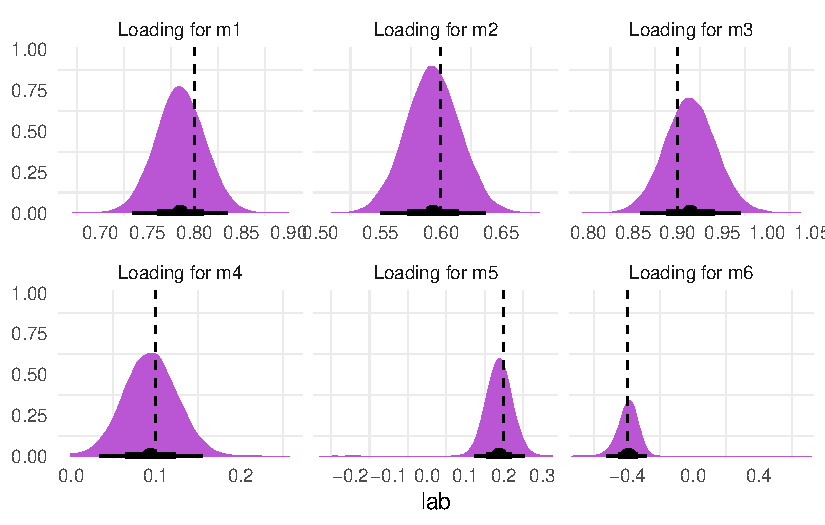
\includegraphics{./bayesian-cfa_files/figure-pdf/viz-draws-mtmm-loadings-1.pdf}

}

\end{figure}

And things are looking good for the covariance terms as well:

\begin{Shaded}
\begin{Highlighting}[]
\CommentTok{\# Plot the covariance stuff}
\NormalTok{dplt }\SpecialCharTok{|\textgreater{}}

  \FunctionTok{filter}\NormalTok{(.variable }\SpecialCharTok{\%in\%} \FunctionTok{c}\NormalTok{(}\StringTok{"Covariance for f1 \textasciitilde{} f2"}\NormalTok{, }\StringTok{"Covariance for m1 \textasciitilde{} m4"}\NormalTok{)) }\SpecialCharTok{|\textgreater{}}

  \FunctionTok{ggplot}\NormalTok{(}\FunctionTok{aes}\NormalTok{(}\AttributeTok{x =}\NormalTok{ .value, }\AttributeTok{fill =}\NormalTok{ .variable)) }\SpecialCharTok{+}
  \FunctionTok{stat\_halfeye}\NormalTok{(}\AttributeTok{fill =} \StringTok{"mediumorchid"}\NormalTok{) }\SpecialCharTok{+}
  \FunctionTok{geom\_vline}\NormalTok{(}\FunctionTok{aes}\NormalTok{(}\AttributeTok{xintercept =}\NormalTok{ true\_loading), }\AttributeTok{linetype =} \DecValTok{2}\NormalTok{) }\SpecialCharTok{+} 
  \FunctionTok{scale\_x\_continuous}\NormalTok{(}\AttributeTok{expand =} \FunctionTok{c}\NormalTok{(}\DecValTok{0}\NormalTok{, }\FloatTok{0.015}\NormalTok{)) }\SpecialCharTok{+}
  \FunctionTok{scale\_y\_continuous}\NormalTok{(}\AttributeTok{expand =} \FunctionTok{c}\NormalTok{(}\DecValTok{0}\NormalTok{, }\FloatTok{0.015}\NormalTok{)) }\SpecialCharTok{+}
  \FunctionTok{guides}\NormalTok{(}\AttributeTok{fill =} \StringTok{"none"}\NormalTok{) }\SpecialCharTok{+}
  \FunctionTok{labs}\NormalTok{(}\AttributeTok{x =} \StringTok{"lab"}\NormalTok{,}
     \AttributeTok{y =} \ConstantTok{NULL}\NormalTok{)  }\SpecialCharTok{+}
  \FunctionTok{facet\_wrap}\NormalTok{(}\SpecialCharTok{\textasciitilde{}}\NormalTok{.variable) }\SpecialCharTok{+}
  \FunctionTok{theme\_minimal}\NormalTok{() }\SpecialCharTok{+} 
  \FunctionTok{theme}\NormalTok{(}
    \AttributeTok{panel.grid.major =} \FunctionTok{element\_blank}\NormalTok{(),}
    \AttributeTok{panel.grid.minor =} \FunctionTok{element\_blank}\NormalTok{()}
\NormalTok{  )}
\end{Highlighting}
\end{Shaded}

\begin{figure}[H]

{\centering 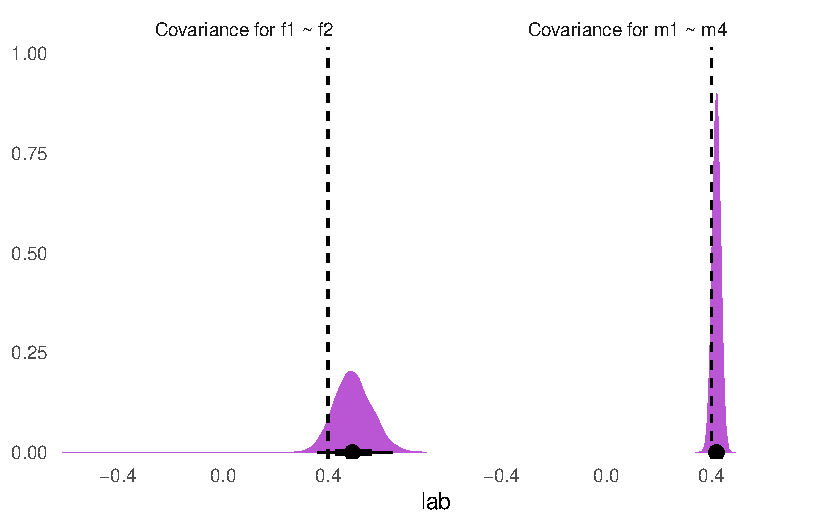
\includegraphics{./bayesian-cfa_files/figure-pdf/viz-draws-mtmm-covar-1.pdf}

}

\end{figure}

Out of curiosity we can also check the MCMC diagnostics. The Rhats and
effective sample sizes are looking a bit healthier than the previous
model, which is interesting considering we've made the model more
complex by adding a new parameter.

\begin{Shaded}
\begin{Highlighting}[]
\NormalTok{draws }\SpecialCharTok{|\textgreater{}}

  \FunctionTok{summary}\NormalTok{() }\SpecialCharTok{|\textgreater{}}

  \FunctionTok{select}\NormalTok{(variable, rhat, ess\_bulk, ess\_tail) }\SpecialCharTok{|\textgreater{}}

  \FunctionTok{mutate}\NormalTok{(}\FunctionTok{across}\NormalTok{(}\FunctionTok{where}\NormalTok{(is.numeric), }\SpecialCharTok{\textasciitilde{}}\FunctionTok{round}\NormalTok{(.x, }\DecValTok{2}\NormalTok{))) }\SpecialCharTok{|\textgreater{}}

\NormalTok{  knitr}\SpecialCharTok{::}\FunctionTok{kable}\NormalTok{()}
\end{Highlighting}
\end{Shaded}

\begin{longtable}[]{@{}lrrr@{}}
\toprule()
variable & rhat & ess\_bulk & ess\_tail \\
\midrule()
\endhead
lam{[}1,1{]} & 1.00 & 4652.90 & 9876.69 \\
lam{[}2,1{]} & 1.00 & 13721.92 & 17472.99 \\
lam{[}3,1{]} & 1.00 & 3707.37 & 6725.97 \\
lam{[}4,2{]} & 1.00 & 4983.17 & 10820.66 \\
lam{[}5,2{]} & 1.00 & 4287.63 & 8968.60 \\
lam{[}6,2{]} & 1.01 & 537.83 & 956.49 \\
Rho\_factors{[}2,1{]} & 1.01 & 400.12 & 569.74 \\
Rho\_m1\_m4{[}2,1{]} & 1.00 & 8851.63 & 14678.11 \\
\bottomrule()
\end{longtable}

The trace plots also look generally healthy, albeit exhibiting a few of
the same big spikes we saw in the previous example.

\begin{Shaded}
\begin{Highlighting}[]
\NormalTok{draws }\SpecialCharTok{|\textgreater{}}

\NormalTok{  bayesplot}\SpecialCharTok{::}\FunctionTok{mcmc\_trace}\NormalTok{() }\SpecialCharTok{+} 
  \FunctionTok{scale\_color\_manual}\NormalTok{(}\AttributeTok{values =} \FunctionTok{c}\NormalTok{(}\StringTok{"blue"}\NormalTok{, }\StringTok{"red"}\NormalTok{, }\StringTok{"orange"}\NormalTok{, }\StringTok{"mediumorchid"}\NormalTok{)) }\SpecialCharTok{+} 
  \FunctionTok{theme\_minimal}\NormalTok{() }\SpecialCharTok{+}
  \FunctionTok{theme}\NormalTok{(}
    \AttributeTok{panel.grid.major =} \FunctionTok{element\_blank}\NormalTok{(),}
    \AttributeTok{panel.grid.minor =} \FunctionTok{element\_blank}\NormalTok{()}
\NormalTok{  )}
\end{Highlighting}
\end{Shaded}

\hypertarget{fourth-example-survival-analysis}{%
\section{Fourth Example: Survival
Analysis}\label{fourth-example-survival-analysis}}

Now that we're confident our CFA MTMM Stan model is well-specified, we
can graft it onto the substantive regression model for the outcome of
interest: time to employment.

The updated model is shown below. All we've done is add two new lines at
the top of the model. These lines say we imagine time-to-event \(T\) for
each person \(i\) to be drawn from a shared Weibull distribution, whose
location parameter is a linear model of the latent factors
\(\text{adapt}\) and \(\text{collab}\), as well as other measured
variables in the matrix \(\mathbf{X}\), each with its own coefficient in
the vector \(\boldsymbol{\beta}\).

\$\$

\begin{aligned}
\color{teal}T_i &\color{teal}\sim \text{Weibull}(\theta_i, k) \\
\color{teal}\theta_i &\color{teal}= \alpha + \beta_1 \text{adapt}_{i} + \beta_2 \text{collab}_{i} + \mathbf{X}_i \boldsymbol{\beta} \\
\\
\begin{bmatrix}
m_{1} \\
m_{2} \\
m_{3} \\
m_{4} \\
m_{5} \\
m_{6}
\end{bmatrix}
&\sim \text{MVNormal}
\left(
\begin{bmatrix}
\mu_{m1} \\
\mu_{m2} \\
\mu_{m3} \\
\mu_{m4} \\
\mu_{m5} \\
\mu_{m6}
\end{bmatrix},
\Sigma_m
\right) \\
\\
\mu_{m1} &= \lambda_1 \text{adapt}, \quad \mu_{m2} = \lambda_2 \text{adapt}, \quad \mu_{m3} = \lambda_3 \text{adapt} \\
\mu_{m4} &= \lambda_4 \text{collab}, \quad \mu_{m5} = \lambda_5 \text{collab}, \quad \mu_{m6} = \lambda_6 \text{collab} \\
\\
\begin{bmatrix}
\text{adapt}_{i} \\
\text{collab}_{i}
\end{bmatrix}
&\sim \text{MVNormal}
\left(
\begin{bmatrix}
\mu_\text{adapt} \\
\mu_\text{collab}
\end{bmatrix},
\Sigma_f
\right) \\
\\
\Sigma_f &=
\begin{bmatrix}
\sigma_\text{adapt}^2 & \color{orchid}{\rho \sigma_\text{adapt} \sigma_\text{collab}} \\
\color{orchid}{\rho \sigma_\text{adapt} \sigma_\text{collab}} & \sigma_\text{adapt}^2
\end{bmatrix}
\\
\Sigma_m &=
\begin{bmatrix}
\sigma_{m1}^2 & 0 & 0 & \color{orange}{\rho\ \sigma_{m1} \sigma_{m4}} & 0 & 0 \\
0 & \sigma_{m2}^2 & 0 & 0 & 0 & 0 \\
0 & 0 & \sigma_{m3}^2 & 0 & 0 & 0 \\
\color{orange}{\rho \sigma_{m1} \sigma_{m4}} & 0 & 0 & \sigma_{m4}^2 & 0 & 0 \\
0 & 0 & 0 & 0 & \sigma_{m5}^2 & 0 \\
0 & 0 & 0 & 0 & 0 & \sigma_{m6}^2
\end{bmatrix}
\end{aligned}

\$\$

Why a Weibull likelihood? According to Collett (2003), this is a common
choice for parameteric survival analysis because it corresponds to a
flexible monotonic baseline hazard function, which often feels like a
safe assumption that is neither too rigid (like an exponential
likelihood and corresponding flat baseline hazard function) nor too
flexible (like a spline with many knots). It also has the advantage of
being interpretable as either a Proportional Hazards regression or as an
Accelerated Failure Time regression, which gives us flexibility in how
we communicate about the parameter estimates, and allows us to not worry
too much about the proportional hazards assumption.

\hypertarget{data-simulation-and-validation}{%
\subsection{Data Simulation and
Validation}\label{data-simulation-and-validation}}

Unlike in previous sections, here we won't be able to rely on
\texttt{lavaan::simulateData()} to create our simulated data, because it
can't generate time-to-event data. So we'll need to generate the data
ourselves.
\href{https://scholar.google.com/citations?user=s2LhwXAAAAAJ\&hl=en}{Mark
Lai} has shared
\href{https://bookdown.org/marklhc/notes/simulation-example-on-structural-equation-modeling-sem.html\#full-example-of-a-small-scale-simulation}{some
nice code} to do this. I use his approach, adapting it slightly allow
for covariance between m1 and m4 as in the MTMM model above. For now
we'll simulate the measured variables as continuous and gaussian, even
though it is more realistic that in this context they would be ordinal
likert-style.

\begin{Shaded}
\begin{Highlighting}[]
\CommentTok{\# Define sample size}
\NormalTok{N }\OtherTok{\textless{}{-}} \DecValTok{4000}

\CommentTok{\# Define the Fixed Parameters}
\NormalTok{alpha }\OtherTok{\textless{}{-}} \FunctionTok{c}\NormalTok{(}\DecValTok{0}\NormalTok{, }\DecValTok{0}\NormalTok{)  }\CommentTok{\# latent means}

\CommentTok{\# latent variances/covariances}
\NormalTok{Phi }\OtherTok{\textless{}{-}} \FunctionTok{matrix}\NormalTok{(}\FunctionTok{c}\NormalTok{(}\DecValTok{1}\NormalTok{, }\FloatTok{0.4}\NormalTok{, }
                \FloatTok{0.4}\NormalTok{, }\DecValTok{1}\NormalTok{), }\AttributeTok{nrow =} \DecValTok{2}\NormalTok{)  }

\CommentTok{\# factor loadings}
\NormalTok{Lambda }\OtherTok{\textless{}{-}} \FunctionTok{cbind}\NormalTok{(}\FunctionTok{c}\NormalTok{(.}\DecValTok{8}\NormalTok{, .}\DecValTok{6}\NormalTok{, .}\DecValTok{9}\NormalTok{, }\DecValTok{0}\NormalTok{, }\DecValTok{0}\NormalTok{, }\DecValTok{0}\NormalTok{), }
                \FunctionTok{c}\NormalTok{(}\DecValTok{0}\NormalTok{, }\DecValTok{0}\NormalTok{, }\DecValTok{0}\NormalTok{, .}\DecValTok{1}\NormalTok{, .}\DecValTok{2}\NormalTok{, }\SpecialCharTok{{-}}\NormalTok{.}\DecValTok{4}\NormalTok{))  }

\CommentTok{\# Error structure of measured variables}
\NormalTok{Theta }\OtherTok{\textless{}{-}} \FunctionTok{diag}\NormalTok{(}\FunctionTok{c}\NormalTok{(}\FunctionTok{c}\NormalTok{(}\DecValTok{1}\NormalTok{, }\DecValTok{1}\NormalTok{, }\DecValTok{1}\NormalTok{, }\DecValTok{1}\NormalTok{, }\DecValTok{1}\NormalTok{, }\DecValTok{1}\NormalTok{)))}
\NormalTok{Theta[}\DecValTok{4}\NormalTok{, }\DecValTok{1}\NormalTok{] }\OtherTok{\textless{}{-}}\NormalTok{ .}\DecValTok{4}
\NormalTok{Theta[}\DecValTok{1}\NormalTok{, }\DecValTok{4}\NormalTok{] }\OtherTok{\textless{}{-}}\NormalTok{ .}\DecValTok{4}

\CommentTok{\# Generate latent factor scores}
\NormalTok{eta }\OtherTok{\textless{}{-}}\NormalTok{ MASS}\SpecialCharTok{::}\FunctionTok{mvrnorm}\NormalTok{(N, }\AttributeTok{mu =}\NormalTok{ alpha, }\AttributeTok{Sigma =}\NormalTok{ Phi)}

\CommentTok{\# Generate residuals}
\NormalTok{e }\OtherTok{\textless{}{-}}\NormalTok{ MASS}\SpecialCharTok{::}\FunctionTok{mvrnorm}\NormalTok{(N, }\AttributeTok{mu =} \FunctionTok{rep}\NormalTok{(}\DecValTok{0}\NormalTok{, }\DecValTok{6}\NormalTok{), }\AttributeTok{Sigma =}\NormalTok{ Theta)}

\CommentTok{\# Compute outcome scores: m\_i = t(Lambda \%*\% eta\_i) + e}
\NormalTok{m }\OtherTok{\textless{}{-}} \FunctionTok{tcrossprod}\NormalTok{(eta, Lambda) }\SpecialCharTok{+}\NormalTok{ e}

\CommentTok{\# Pack the measured variables and factor scores into a dataset}
\NormalTok{fake\_dat\_measurement }\OtherTok{\textless{}{-}} \FunctionTok{tibble}\NormalTok{(}
  \AttributeTok{m1 =}\NormalTok{ m[,}\DecValTok{1}\NormalTok{],}
  \AttributeTok{m2 =}\NormalTok{ m[,}\DecValTok{2}\NormalTok{],}
  \AttributeTok{m3 =}\NormalTok{ m[,}\DecValTok{3}\NormalTok{],}
  \AttributeTok{m4 =}\NormalTok{ m[,}\DecValTok{4}\NormalTok{],}
  \AttributeTok{m5 =}\NormalTok{ m[,}\DecValTok{5}\NormalTok{],}
  \AttributeTok{m6 =}\NormalTok{ m[,}\DecValTok{6}\NormalTok{],}
  \AttributeTok{adapt =}\NormalTok{ eta[,}\DecValTok{1}\NormalTok{],}
  \AttributeTok{collab =}\NormalTok{ eta[,}\DecValTok{2}\NormalTok{]}
\NormalTok{)}
\end{Highlighting}
\end{Shaded}

Now we have our `measured' variables, simulated according to our chosen
factor loadings and error structure. Just to be safe, let's make sure
lavaan can recover the true parameter estimates. We need to specify
\texttt{std.lv\ =\ TRUE} to override lavaan's default behaviour of using
the marker variable approach for identifiability, and instead fix the
variances of the latent variables to 1. If we don't do this then the
model doesn't return the true simulated parameter estimates because the
scales of the latent variables get messed up. Looks like lavaan can
recover the true parameter estimates, which means our data simulation
code does what we think it does:

\begin{Shaded}
\begin{Highlighting}[]
\NormalTok{surv.measurement.model }\OtherTok{\textless{}{-}} \StringTok{\textquotesingle{} }
\StringTok{  f1 =\textasciitilde{} m1 + m2 + m3}
\StringTok{  f2 =\textasciitilde{} m4 + m5 + m6}

\StringTok{  f1 \textasciitilde{}\textasciitilde{} f1}
\StringTok{  f2 \textasciitilde{}\textasciitilde{} f2}

\StringTok{  m1 \textasciitilde{}\textasciitilde{} m4}
\StringTok{\textquotesingle{}}

\CommentTok{\# Fit the model}
\NormalTok{fit\_test }\OtherTok{\textless{}{-}} \FunctionTok{cfa}\NormalTok{(surv.measurement.model, }\AttributeTok{data =}\NormalTok{ fake\_dat\_measurement }\SpecialCharTok{|\textgreater{}} \FunctionTok{select}\NormalTok{(}\FunctionTok{starts\_with}\NormalTok{(}\StringTok{"m"}\NormalTok{)), }\AttributeTok{std.lv =} \ConstantTok{TRUE}\NormalTok{)}

\CommentTok{\# Make sure it works}
\NormalTok{fit\_test }\SpecialCharTok{|\textgreater{}} 

\NormalTok{  broom}\SpecialCharTok{::}\FunctionTok{tidy}\NormalTok{() }\SpecialCharTok{|\textgreater{}}

  \FunctionTok{select}\NormalTok{(term, estimate) }\SpecialCharTok{|\textgreater{}}

\NormalTok{  knitr}\SpecialCharTok{::}\FunctionTok{kable}\NormalTok{()}
\end{Highlighting}
\end{Shaded}

\begin{longtable}[]{@{}lr@{}}
\toprule()
term & estimate \\
\midrule()
\endhead
f1 =\textasciitilde{} m1 & 0.8031530 \\
f1 =\textasciitilde{} m2 & 0.5989194 \\
f1 =\textasciitilde{} m3 & 0.9033436 \\
f2 =\textasciitilde{} m4 & 0.1157250 \\
f2 =\textasciitilde{} m5 & 0.2158621 \\
f2 =\textasciitilde{} m6 & -0.3541507 \\
f1 \textasciitilde\textasciitilde{} f1 & 1.0000000 \\
f2 \textasciitilde\textasciitilde{} f2 & 1.0000000 \\
m1 \textasciitilde\textasciitilde{} m4 & 0.4022579 \\
m1 \textasciitilde\textasciitilde{} m1 & 0.9769983 \\
m2 \textasciitilde\textasciitilde{} m2 & 1.0156702 \\
m3 \textasciitilde\textasciitilde{} m3 & 0.9648986 \\
m4 \textasciitilde\textasciitilde{} m4 & 1.0062068 \\
m5 \textasciitilde\textasciitilde{} m5 & 1.0382976 \\
m6 \textasciitilde\textasciitilde{} m6 & 1.0372607 \\
f1 \textasciitilde\textasciitilde{} f2 & 0.5369498 \\
\bottomrule()
\end{longtable}

Now we can simulate the demographic variables and time-to-event data
using the CFA data we simulated above. We can draw the covariates
straightforwardly from the relevent distributions, but the
times-to-event will require a bit more thought. There are existing
packages for simulating survival data in R (such as
\href{https://cran.r-project.org/web/packages/simsurv/vignettes/simsurv_usage.html}{simsurv}
by Sam Brilleman of rstanarm fame!) but since we're taking an explicit
approach for the latent variables this time, it's nice to continue in
that fashion for the entire dataset. I found
\href{https://stats.stackexchange.com/a/472260/337075}{this Stack
Exchange answer} by user
\href{https://stats.stackexchange.com/users/206635/ryan-sy-kwan}{Ryan SY
Kwan} helpful for learning an explicit workflow for simulating survival
data from a Weibull distribution, which I implement here.

The goal is to find a way of expressing the Weibull distribution's shape
parameter with reference to the linear model, so that we can use R's
built-in \texttt{rweibull()} function to sample our event times. We can
start from \href{https://en.wikipedia.org/wiki/Weibull_distribution}{the
PDF of the Weibull distribution}:

\$\$

\begin{equation}
f(x; k, \lambda) = \begin{cases}
\frac{k}{\lambda} \left( \frac{x}{\lambda} \right)^{k-1} e^{-(x/\lambda)^{k}} & x > 0, \\
0 & x \leq 0.
\end{cases}
\end{equation}

\$\$

And its cumulative density function given by:

\$\$

\begin{equation}
F(x; k, \lambda) = 1 - \exp\left(-\left(\frac{x}{\lambda}\right)^{k}\right)
\end{equation}

\$\$

So the survival curve, given by 1 - CDF, is:

\$\$

\begin{equation}
S(x; k, \lambda) = \exp\left(-\left(\frac{x}{\lambda}\right)^{k}\right)
\end{equation}

\$\$

And using the classic negative-log relationship between the survival
function and the cumulative hazard function, we can say:

\$\$

\begin{equation}
H(t) = -\log\left(\exp\left(-\left(\frac{t}{\lambda}\right)^{\rho}\right)\right)
\end{equation}

\textbackslash{[}1em{]}

\begin{equation}
H(t) = \left(\frac{t}{\lambda}\right)^{\rho}
\end{equation}

\$\$

Now we have everything we need to implement the the classic form of a
Cox Proportional Hazards regression, given by: \$\$

\begin{equation}
H(t | \mathbf{X}) = H_0(t) \exp(\mathbf{\beta}' \mathbf{X})
\end{equation}

\$\$

Since this is directly equivalent to the model for the actual function
of interest, the baseline hazard. As Singer and Willett (2003) put it,
\emph{``This direct equivalence may not be intuitive, but it certainly
is invaluable.''}

\$\$

\begin{equation}
h(t | \mathbf{X}) = h_0(t) \exp(\mathbf{\beta}' \mathbf{X})
\end{equation}

\$\$

So we can take the definition of the Weibull cumulative hazard function
we found above and substitute it into this equation, then take its
negative exp to get it back in terms of the survival function:

\$\$

\begin{equation}
S(t \mid \mathbf{x}) = \exp\left(-\left(\frac{t}{\lambda}\right)^{\rho} \exp(\mathbf{\beta}' \mathbf{x})\right)
\end{equation}

\$\$

Now we can rearrange things to make the scale parameter \(\lambda\)
itself a function of the linear model. This allows us to use R's
built-in \texttt{rweibull()} function to generate the event times. All
we need is some fancy algebra:

\$\$

\begin{align*}
S(t \mid x, \lambda) &= \exp\left(-\left(\frac{t}{\lambda}\right)^{\rho} \exp(x' \beta)\right) \\
&= \exp\left(-\left(\frac{t}{\lambda}\right)^{\rho} \exp\left(\frac{x' \beta}{\rho}\right)\rho\right) \\
&= \exp\left(-\left(\frac{t}{\frac{\lambda}{\exp\left(\frac{x' \beta}{\rho}\right)}}\right)^{\rho}\right) \\
\end{align*}

\$\$

Now the denominator incorporates both \(\lambda\) and the linear model.
So we can just take the whole denominator and call it its own new thing
\(\lambda'\):

\$\$

\begin{align*}
\lambda' = \frac{\lambda}{\exp\left(\frac{x' \beta}{\rho}\right)}
\end{align*}

\$\$

Thus we've snuck our linear model into the classic no-model definition
of the Weibull survival function we saw above, just with \(\lambda'\)
instead of \(\lambda\):

\$\$

\begin{equation}
S(x; k, \lambda) = \exp\left(-\left(\frac{x}{\lambda'}\right)^{k}\right)
\end{equation}

\$\$

This is the parameterization we can implement when we go to create our
event times. We'll also imagine censoring times to be drawn from an
unconditional exponential distribution, which creates non-informative
censoring. We'll generate an event time and a censoring time for each
person, and a person's status will be the shorter of those two times. We
can start by choosing values for the Weibull distribution's \texttt{rho}
and \texttt{lambda} parameters that generate a realistic-seeming
distribution of times-to-employment in the absence of a linear model.
This is simpler conceptually if we define \texttt{rho\ =\ 1}. After some
trial and error I settled on \texttt{lambda\ =\ .02}, which results in a
mean time-to-employment of 22 days in the simulated dataset.

Now we can choose the simulated parameter estimates for the linear
model. There's some tricky conversion we need to do to interpret our
parametric estimates when we use the survival function, because the
Weibull (and exponential, which is a special case of Weibull) results
have the magic property of being able to be interpreted either as hazard
ratios \emph{or} acceleration factors.
\href{https://rstudio-pubs-static.s3.amazonaws.com/5564_bc9e2d9a458c4660aa82882df90b7a6b.html}{This
nice markdown document} provides a walkthrough of the transformations
required to move between these two interpretations. The canonical
\textbf{survival} package implements Weibull regression as an
accelerated failure time model by default, and I find this
interpretation more user-friendly so I will stick with it for our
purposes here. But in declaring the simulation parameter estimates we
need to keep in mind that there are two different but equivalent ways of
transforming the parameter estimates when interpretting the results of
this sort of model. Brilleman et al. (2020) provide a clear overview:

\begin{itemize}
\tightlist
\item
  \(\exp(-\beta_p(t))\) is an \textbf{acceleration factor}: Sub-zero
  values of the transformed parameter estimates correspond to
  \emph{slower} event times.
\item
  \(\exp(\beta_p(t))\) is a \textbf{survival time ratio}: Sub-zero
  values of the transformed parameter estimates correspond to
  \emph{faster} event times.
\end{itemize}

This is important to keep in mind when we declare our `true' simulation
parameter estimates. We can declare them as survival time ratios for
simplicity when implementing the simulation, even though the
\{\{survival\}\} package and Stan will return acceleration factors by
default. For example, for this simulation we can imagine that being on
employment insurance is associated with twice-as-fast time-to-employment
because it means you have recent work experience. We simulate this by
setting the coefficient \texttt{beta\_ie\ \textless{}-\ log(2)}, which
corresponds to an acceleration factor of .5. Likewise, we can imagine
that a one-unit increase in the latent trait `Collaboration Skills' is
associated with 20\% faster job attainment, so we set
\texttt{beta\_collab\ \textless{}-\ log(1.2)}, which corresponds to an
acceleration factor of
\texttt{exp(-log(1.2))\ \textasciitilde{}\ 0.833}. We can proceed in the
same way for the other parameter estimates.

\begin{Shaded}
\begin{Highlighting}[]
\CommentTok{\# Declare some parameter values for baseline hazard}
\NormalTok{lambda }\OtherTok{\textless{}{-}}\NormalTok{ .}\DecValTok{02}
\NormalTok{rho }\OtherTok{\textless{}{-}} \DecValTok{1} \CommentTok{\# keep rho = 1 to keep the conversions simple / make it easier to specify lambda}
\NormalTok{lambda\_wiki }\OtherTok{\textless{}{-}}\NormalTok{ lambda}\SpecialCharTok{\^{}}\NormalTok{(}\SpecialCharTok{{-}}\DecValTok{1} \SpecialCharTok{/}\NormalTok{ rho) }

\CommentTok{\# Declare some true linear model parameters}
\NormalTok{beta\_adapt }\OtherTok{\textless{}{-}} \FunctionTok{log}\NormalTok{(}\DecValTok{1}\NormalTok{) }\CommentTok{\# adaptability skills have no effect on time{-}to{-}employment}
\NormalTok{beta\_collab }\OtherTok{\textless{}{-}} \FunctionTok{log}\NormalTok{(}\FloatTok{1.2}\NormalTok{) }\CommentTok{\# collaboration skills decrease time{-}to{-}employment by 20\% for each standard deviation increase.}
\NormalTok{beta\_age }\OtherTok{\textless{}{-}} \FunctionTok{log}\NormalTok{(.}\DecValTok{9}\NormalTok{) }\CommentTok{\# older people find employment a bit slower {-}{-} each increase in age of 1 standard deviation slows time{-}to{-}employment to 90\% of what is was previously.}
\NormalTok{beta\_ei }\OtherTok{\textless{}{-}} \FunctionTok{log}\NormalTok{(}\DecValTok{2}\NormalTok{) }\CommentTok{\# people on EI find employment twice as fast }

\CommentTok{\# Declare the rate for the exponential distribution from which we will sample censoring times}
\NormalTok{censor\_rate }\OtherTok{=}\NormalTok{ .}\DecValTok{02}

\CommentTok{\# Simulate the covariates and event times}
\NormalTok{fake\_dat }\OtherTok{\textless{}{-}}\NormalTok{ fake\_dat\_measurement }\SpecialCharTok{|\textgreater{}}

  \FunctionTok{rowid\_to\_column}\NormalTok{() }\SpecialCharTok{|\textgreater{}}

  \FunctionTok{mutate}\NormalTok{(}

    \CommentTok{\# Simulate the covariates}
    \AttributeTok{age =} \FunctionTok{rnorm}\NormalTok{(N), }
    \AttributeTok{ei\_status =} \FunctionTok{rbinom}\NormalTok{(N, }\DecValTok{1}\NormalTok{, .}\DecValTok{4}\NormalTok{),}
    \AttributeTok{n\_previous\_programs =} \FunctionTok{sample}\NormalTok{(}\FunctionTok{c}\NormalTok{(}\DecValTok{1}\NormalTok{, }\DecValTok{2}\NormalTok{, }\DecValTok{3}\NormalTok{, }\DecValTok{4}\NormalTok{), N, }\AttributeTok{prob =} \FunctionTok{c}\NormalTok{(.}\DecValTok{5}\NormalTok{, .}\DecValTok{3}\NormalTok{, .}\DecValTok{15}\NormalTok{, .}\DecValTok{05}\NormalTok{), }\AttributeTok{replace =} \ConstantTok{TRUE}\NormalTok{)}

\NormalTok{  ) }\SpecialCharTok{|\textgreater{}}

  \FunctionTok{group\_by}\NormalTok{(rowid) }\SpecialCharTok{|\textgreater{}}

  \FunctionTok{mutate}\NormalTok{(}

    \CommentTok{\# Simulate the event times and censoring times}
    \AttributeTok{lambda\_prime =}\NormalTok{ lambda\_wiki }\SpecialCharTok{/} \FunctionTok{exp}\NormalTok{((beta\_adapt}\SpecialCharTok{*}\NormalTok{adapt }\SpecialCharTok{+}\NormalTok{ beta\_collab}\SpecialCharTok{*}\NormalTok{collab }\SpecialCharTok{+}\NormalTok{ beta\_age}\SpecialCharTok{*}\NormalTok{age }\SpecialCharTok{+}\NormalTok{ beta\_ei}\SpecialCharTok{*}\NormalTok{ei\_status) }\SpecialCharTok{/}\NormalTok{ rho),}
    \AttributeTok{time\_event =} \FunctionTok{rweibull}\NormalTok{(}\DecValTok{1}\NormalTok{, }\AttributeTok{shape=}\NormalTok{rho, }\AttributeTok{scale=}\NormalTok{lambda\_prime),}
    \AttributeTok{time\_censor =} \FunctionTok{rexp}\NormalTok{(}\DecValTok{1}\NormalTok{, censor\_rate),}
    \AttributeTok{time =} \FunctionTok{min}\NormalTok{(time\_event, time\_censor),}
    \AttributeTok{censored =} \FunctionTok{ifelse}\NormalTok{(time\_censor }\SpecialCharTok{\textless{}=}\NormalTok{ time\_event, }\DecValTok{1}\NormalTok{, }\DecValTok{0}\NormalTok{),}
    \AttributeTok{status =} \FunctionTok{ifelse}\NormalTok{(time\_censor }\SpecialCharTok{\textgreater{}}\NormalTok{ time\_event, }\DecValTok{1}\NormalTok{, }\DecValTok{0}\NormalTok{)}

\NormalTok{  ) }\SpecialCharTok{|\textgreater{}}

  \FunctionTok{ungroup}\NormalTok{() }\SpecialCharTok{|\textgreater{}}

  \CommentTok{\# Remove the intermediary variables we don\textquotesingle{}t need}
  \FunctionTok{select}\NormalTok{(}\SpecialCharTok{{-}}\FunctionTok{c}\NormalTok{(}
\NormalTok{    lambda\_prime,}
\NormalTok{    time\_event,}
\NormalTok{    time\_censor}
\NormalTok{  ))}

\NormalTok{fake\_dat }\SpecialCharTok{|\textgreater{}}

  \FunctionTok{summarize}\NormalTok{(}\AttributeTok{what =} \FunctionTok{mean}\NormalTok{(time))}
\end{Highlighting}
\end{Shaded}

\begin{verbatim}
# A tibble: 1 x 1
   what
  <dbl>
1  21.7
\end{verbatim}

If we've done everything correctly then a basic survival analysis should
be able to recover the true parameter estimates using the true model
specification. Indeed, this is what we see:

\begin{Shaded}
\begin{Highlighting}[]
\CommentTok{\# Create the surv object}
\NormalTok{surv\_object }\OtherTok{\textless{}{-}} \FunctionTok{Surv}\NormalTok{(fake\_dat}\SpecialCharTok{$}\NormalTok{time, fake\_dat}\SpecialCharTok{$}\NormalTok{status)}

\CommentTok{\# Fit the model using the surv object}
\NormalTok{test }\OtherTok{\textless{}{-}} \FunctionTok{survreg}\NormalTok{(surv\_object }\SpecialCharTok{\textasciitilde{}}\NormalTok{ adapt }\SpecialCharTok{+}\NormalTok{ collab }\SpecialCharTok{+}\NormalTok{ age }\SpecialCharTok{+}\NormalTok{ ei\_status, }\AttributeTok{data=}\NormalTok{fake\_dat, }\AttributeTok{dist=}\StringTok{\textquotesingle{}weibull\textquotesingle{}}\NormalTok{)}

\CommentTok{\# Wrangle and plot}
\NormalTok{tidied\_results }\OtherTok{\textless{}{-}}\NormalTok{ test }\SpecialCharTok{|\textgreater{}} 
  
\NormalTok{  broom}\SpecialCharTok{::}\FunctionTok{tidy}\NormalTok{(}\AttributeTok{conf.int =} \ConstantTok{TRUE}\NormalTok{) }\SpecialCharTok{|\textgreater{}}

  \FunctionTok{mutate}\NormalTok{(}
    \AttributeTok{estimate =} \FunctionTok{exp}\NormalTok{(estimate),}
    \AttributeTok{conf.low =} \FunctionTok{exp}\NormalTok{(conf.low),}
    \AttributeTok{conf.high =} \FunctionTok{exp}\NormalTok{(conf.high)}
\NormalTok{  ) }\SpecialCharTok{|\textgreater{}}

  \FunctionTok{filter}\NormalTok{(}\SpecialCharTok{!}\NormalTok{term }\SpecialCharTok{\%in\%} \FunctionTok{c}\NormalTok{(}\StringTok{"(Intercept)"}\NormalTok{, }\StringTok{"Log(scale)"}\NormalTok{)) }\SpecialCharTok{|\textgreater{}}

  \FunctionTok{mutate}\NormalTok{(}\AttributeTok{true\_loading =} \FunctionTok{case\_when}\NormalTok{(}
\NormalTok{    term }\SpecialCharTok{==} \StringTok{"age"} \SpecialCharTok{\textasciitilde{}} \FloatTok{1.11}\NormalTok{,}
\NormalTok{    term }\SpecialCharTok{==} \StringTok{"collab"} \SpecialCharTok{\textasciitilde{}} \FloatTok{0.833}\NormalTok{,}
\NormalTok{    term }\SpecialCharTok{==} \StringTok{"adapt"} \SpecialCharTok{\textasciitilde{}} \DecValTok{1}\NormalTok{,}
\NormalTok{    term }\SpecialCharTok{==} \StringTok{"ei\_status"} \SpecialCharTok{\textasciitilde{}} \FloatTok{0.5}
\NormalTok{  )) }\SpecialCharTok{|\textgreater{}}

  \FunctionTok{ggplot}\NormalTok{(}\FunctionTok{aes}\NormalTok{(}\AttributeTok{x =} \FunctionTok{reorder}\NormalTok{(term, }\SpecialCharTok{{-}}\NormalTok{estimate), }\AttributeTok{y =}\NormalTok{ estimate)) }\SpecialCharTok{+}
    \FunctionTok{geom\_point}\NormalTok{() }\SpecialCharTok{+}
    \FunctionTok{geom\_linerange}\NormalTok{(}\FunctionTok{aes}\NormalTok{(}\AttributeTok{ymin =}\NormalTok{ conf.low, }\AttributeTok{ymax =}\NormalTok{ conf.high), }\AttributeTok{size =} \DecValTok{2}\NormalTok{, }\AttributeTok{colour =}   \StringTok{"cornflowerblue"}\NormalTok{) }\SpecialCharTok{+}
    \FunctionTok{geom\_point}\NormalTok{(}\AttributeTok{size =} \DecValTok{5}\NormalTok{, }\AttributeTok{colour =} \StringTok{"cornflowerblue"}\NormalTok{) }\SpecialCharTok{+}
    \FunctionTok{geom\_point}\NormalTok{(}\AttributeTok{size =} \DecValTok{3}\NormalTok{, }\AttributeTok{color =} \StringTok{"white"}\NormalTok{) }\SpecialCharTok{+}
    \FunctionTok{geom\_point}\NormalTok{(}\FunctionTok{aes}\NormalTok{(}\AttributeTok{x =}\NormalTok{ term, }\AttributeTok{y =}\NormalTok{ true\_loading), }\AttributeTok{colour =} \StringTok{"red4"}\NormalTok{, }\AttributeTok{size =} \DecValTok{5}\NormalTok{, }\AttributeTok{shape =}  \DecValTok{13}\NormalTok{, }\AttributeTok{stroke =} \DecValTok{1}\NormalTok{) }\SpecialCharTok{+}
    \FunctionTok{coord\_flip}\NormalTok{() }\SpecialCharTok{+} 
    \FunctionTok{labs}\NormalTok{(}
      \AttributeTok{y =} \StringTok{"Estimate"}\NormalTok{,}
      \AttributeTok{x =} \StringTok{"Variable"}
\NormalTok{    ) }\SpecialCharTok{+}
    \FunctionTok{theme\_minimal}\NormalTok{() }
\end{Highlighting}
\end{Shaded}

We can also do some basic exploratory analysis of the data to make sure
the event times make sense:

\begin{Shaded}
\begin{Highlighting}[]
\NormalTok{fake\_dat }\SpecialCharTok{|\textgreater{}}

  \FunctionTok{mutate}\NormalTok{(}\AttributeTok{mean =} \FunctionTok{mean}\NormalTok{(time)) }\SpecialCharTok{|\textgreater{}}

  \FunctionTok{ggplot}\NormalTok{() }\SpecialCharTok{+} 
  \FunctionTok{geom\_histogram}\NormalTok{(}\FunctionTok{aes}\NormalTok{(}\AttributeTok{x =}\NormalTok{ time), }\AttributeTok{colour =} \DecValTok{1}\NormalTok{, }\AttributeTok{fill =} \StringTok{"cornflowerblue"}\NormalTok{) }\SpecialCharTok{+}
  \FunctionTok{geom\_vline}\NormalTok{(}\FunctionTok{aes}\NormalTok{(}\AttributeTok{xintercept =}\NormalTok{ mean), }\AttributeTok{size =} \DecValTok{2}\NormalTok{, }\AttributeTok{linetype =} \DecValTok{2}\NormalTok{) }\SpecialCharTok{+}
  \FunctionTok{scale\_x\_continuous}\NormalTok{(}\AttributeTok{limits =} \FunctionTok{c}\NormalTok{(}\DecValTok{3}\NormalTok{, }\DecValTok{180}\NormalTok{), }\AttributeTok{n.breaks =} \DecValTok{10}\NormalTok{, }\AttributeTok{expand=}\FunctionTok{c}\NormalTok{(}\DecValTok{0}\NormalTok{, }\DecValTok{0}\NormalTok{)) }\SpecialCharTok{+}
  \FunctionTok{scale\_y\_continuous}\NormalTok{(}\AttributeTok{expand=}\FunctionTok{c}\NormalTok{(}\DecValTok{0}\NormalTok{, }\DecValTok{0}\NormalTok{)) }\SpecialCharTok{+}
  \FunctionTok{labs}\NormalTok{(}
    \AttributeTok{x =} \StringTok{"Days to Employment"}\NormalTok{,}
    \AttributeTok{y =} \StringTok{"N Graduates"}
\NormalTok{  ) }\SpecialCharTok{+}
  \FunctionTok{theme\_bw}\NormalTok{() }\SpecialCharTok{+}
  \FunctionTok{theme}\NormalTok{(}
    \AttributeTok{axis.ticks.y =} \FunctionTok{element\_blank}\NormalTok{(),}
    \AttributeTok{panel.grid.major =} \FunctionTok{element\_blank}\NormalTok{(),}
    \AttributeTok{panel.grid.minor =} \FunctionTok{element\_blank}\NormalTok{(),}
    \AttributeTok{axis.text.y =} \FunctionTok{element\_blank}\NormalTok{()}
\NormalTok{  )}
\end{Highlighting}
\end{Shaded}

\begin{figure}[H]

{\centering 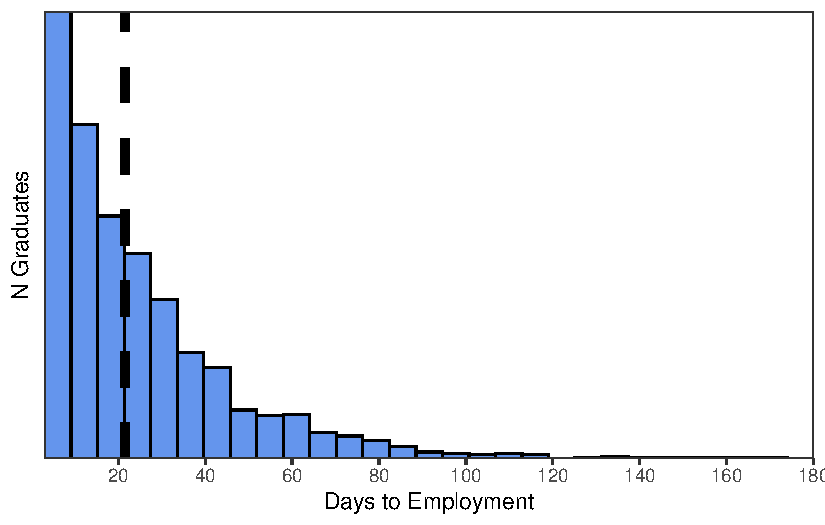
\includegraphics{./bayesian-cfa_files/figure-pdf/viz-raw-event-times-1.pdf}

}

\caption{Histogram of times-to-event, including both events and
censorings.}

\end{figure}

And we can plot some stratified kaplan-meier curves to make sure
parameter estimates mean what we think they mean. For example, we see
that when we stratify by \texttt{ei\_status} those with
\texttt{ei\_status\ ==\ TRUE} see faster estimated event times, which is
what we intended when simulating the data:

\begin{Shaded}
\begin{Highlighting}[]
\NormalTok{km.object }\OtherTok{\textless{}{-}} \FunctionTok{survfit}\NormalTok{(surv\_object }\SpecialCharTok{\textasciitilde{}} \DecValTok{1} \SpecialCharTok{+}\NormalTok{ ei\_status, }\AttributeTok{data =}\NormalTok{ fake\_dat)}

\NormalTok{plt }\OtherTok{\textless{}{-}}\NormalTok{ survminer}\SpecialCharTok{::}\FunctionTok{ggsurvplot}\NormalTok{(}
  \AttributeTok{fit =}\NormalTok{ km.object,}
  \AttributeTok{conf.int =} \ConstantTok{TRUE}\NormalTok{,}
  \AttributeTok{risk.table =} \ConstantTok{FALSE}\NormalTok{,}
  \AttributeTok{legend =} \StringTok{"none"}\NormalTok{,}
  \AttributeTok{palette =} \FunctionTok{c}\NormalTok{(}\StringTok{"cornflowerblue"}\NormalTok{, }\StringTok{"mediumorchid"}\NormalTok{),}
  \AttributeTok{title =} \StringTok{""}\NormalTok{,}
  \AttributeTok{xlab =} \StringTok{"Days Since Graduation"}\NormalTok{, }
  \AttributeTok{ylab =} \StringTok{"Proportion Unemployed"}\NormalTok{,}
  \AttributeTok{ggtheme =} \FunctionTok{theme\_bw}\NormalTok{()}
\NormalTok{)  }

\NormalTok{plt}\SpecialCharTok{$}\NormalTok{plot }\SpecialCharTok{+}
  \FunctionTok{scale\_x\_continuous}\NormalTok{(}\AttributeTok{expand =} \FunctionTok{c}\NormalTok{(}\DecValTok{0}\NormalTok{, }\DecValTok{0}\NormalTok{)) }\SpecialCharTok{+}
  \FunctionTok{scale\_y\_continuous}\NormalTok{(}\AttributeTok{expand =} \FunctionTok{c}\NormalTok{(}\DecValTok{0}\NormalTok{, }\DecValTok{0}\NormalTok{)) }\SpecialCharTok{+}
  \FunctionTok{theme}\NormalTok{(}\AttributeTok{panel.grid.major =} \FunctionTok{element\_blank}\NormalTok{())}
\end{Highlighting}
\end{Shaded}

\begin{figure}[H]

{\centering 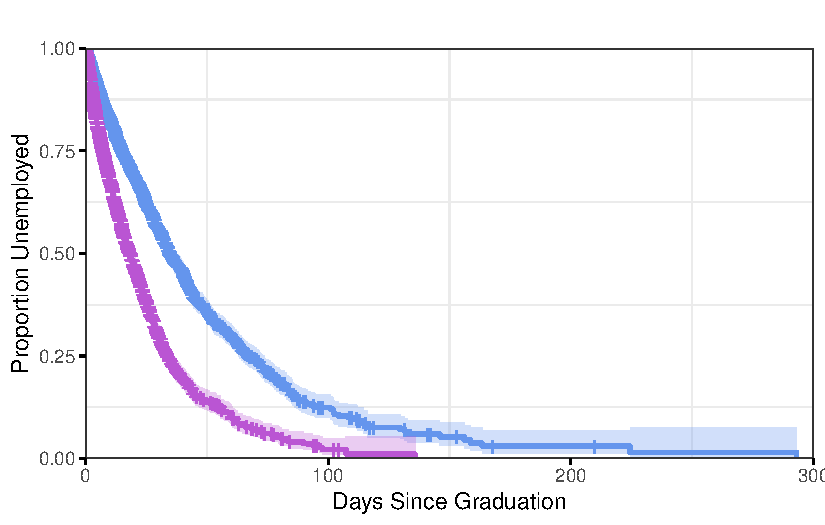
\includegraphics{./bayesian-cfa_files/figure-pdf/viz-km-weibull-1-1.pdf}

}

\caption{Kaplan-Meier estimated survival curves, stratified by EI
Status.}

\end{figure}

\hypertarget{prior-predictive-simulation}{%
\subsection{Prior Predictive
Simulation}\label{prior-predictive-simulation}}

Unlike the factor analysis models we fit above, this model has
substantive predictor variables, namely \texttt{age},
\texttt{ei\_status}, and the two latent variables \texttt{adapt} and
\texttt{collab}. Based on previous research, we have a sense of the
types of parameter estimates that seem realistic for these predictors.
So can use prior predictive simulation to specify informative priors.
Here's what we'll do: 1. Write some simple code to simulate from the
prior distributions of interest; 2. Transform the simulated values to
check whether the priors make sense on the scale of interest; 3. Once we
arrive at reasonable-seeming priors for all of the parameters, we can
use brms to simulate event times from the prior predictive distribution
and make sure everything is making sense.

The brms parameterization of the Weibull distribution
\href{https://cran.r-project.org/web/packages/brms/vignettes/brms_families.html}{is
slightly different} than the one used in the \textbf{survival} package,
with \textbf{brms} specifying a mean parameter as a function of the
scale and shape parameters of the more traditional parameterization:

\$\$

\begin{align*}
s = \frac{\mu}{\Gamma\left(1 + \frac{1}{\alpha}\right)}
\end{align*} \$\$

So when we specify a prior for the intercept term in our Bayesian model,
we're also specifying a prior for this transformation of the scale and
shape parameters under the traditional parameterization:

\$\$

\begin{align*}
\mu = s \times \Gamma\left(1 + \frac{1}{\alpha}\right)
\end{align*}

\$\$

I don't think this has any big implications: setting a prior for the
intercept is more intuitive than setting a prior for the scale and shape
parameters indivdually anyway. We can copy this approach when we go to
fit our Stan model.

Let's start with the prior for the intercept, specifying a prior on the
raw `days-to-employment' scale because that helps keep things
interpretable.

Based on previous studies I've done at my work, an average
time-to-employment of 30 days seems reasonable, and an average higher
than 60 days seems very unlikely. After much trial and error with the
code below it seems like a gaussian with
\texttt{mean\ =\ 3.3,\ sd\ =\ .4} gives a distribution with appropriate
characteristics:

\begin{Shaded}
\begin{Highlighting}[]
\CommentTok{\# Simulate some data}
\NormalTok{sim }\OtherTok{\textless{}{-}} \FunctionTok{rnorm}\NormalTok{(}\DecValTok{10000}\NormalTok{, }\FloatTok{3.3}\NormalTok{, .}\DecValTok{4}\NormalTok{) }\SpecialCharTok{|\textgreater{}}

  \FunctionTok{as\_tibble}\NormalTok{() }\SpecialCharTok{|\textgreater{}}

  \FunctionTok{mutate}\NormalTok{(}\AttributeTok{value =} \FunctionTok{exp}\NormalTok{(value)) }

\CommentTok{\# Get the mean}
\NormalTok{sim }\SpecialCharTok{|\textgreater{}} 

    \FunctionTok{pull}\NormalTok{(value) }\SpecialCharTok{|\textgreater{}}
    
    \FunctionTok{mean}\NormalTok{()}
\end{Highlighting}
\end{Shaded}

\begin{verbatim}
[1] 29.47964
\end{verbatim}

\begin{Shaded}
\begin{Highlighting}[]
\CommentTok{\# Plot the distribution}
\NormalTok{sim }\SpecialCharTok{|\textgreater{}}

    \FunctionTok{ggplot}\NormalTok{(}\FunctionTok{aes}\NormalTok{(}\AttributeTok{x =}\NormalTok{ value)) }\SpecialCharTok{+}
    \FunctionTok{stat\_halfeye}\NormalTok{(}\AttributeTok{fill =} \StringTok{"orchid"}\NormalTok{) }\SpecialCharTok{+}
    \FunctionTok{scale\_x\_continuous}\NormalTok{(}\AttributeTok{n.breaks =} \DecValTok{10}\NormalTok{, }\AttributeTok{expand =} \FunctionTok{c}\NormalTok{(}\DecValTok{0}\NormalTok{, }\DecValTok{0}\NormalTok{)) }\SpecialCharTok{+}
    \FunctionTok{scale\_y\_continuous}\NormalTok{(}\AttributeTok{expand =} \FunctionTok{c}\NormalTok{(}\DecValTok{0}\NormalTok{, }\DecValTok{0}\NormalTok{)) }\SpecialCharTok{+}
    \FunctionTok{labs}\NormalTok{(}
      \AttributeTok{x =} \StringTok{"rnorm draw"}\NormalTok{,}
      \AttributeTok{y =} \StringTok{"Density"}
\NormalTok{    ) }\SpecialCharTok{+}
    \FunctionTok{theme\_bw}\NormalTok{() }\SpecialCharTok{+}
    \FunctionTok{theme}\NormalTok{(}
      \AttributeTok{axis.ticks.y =} \FunctionTok{element\_blank}\NormalTok{(),}
      \AttributeTok{panel.grid.major =} \FunctionTok{element\_blank}\NormalTok{(),}
      \AttributeTok{panel.grid.minor =} \FunctionTok{element\_blank}\NormalTok{(),}
      \AttributeTok{axis.text.y =} \FunctionTok{element\_blank}\NormalTok{()}
\NormalTok{    )}
\end{Highlighting}
\end{Shaded}

\begin{figure}[H]

{\centering 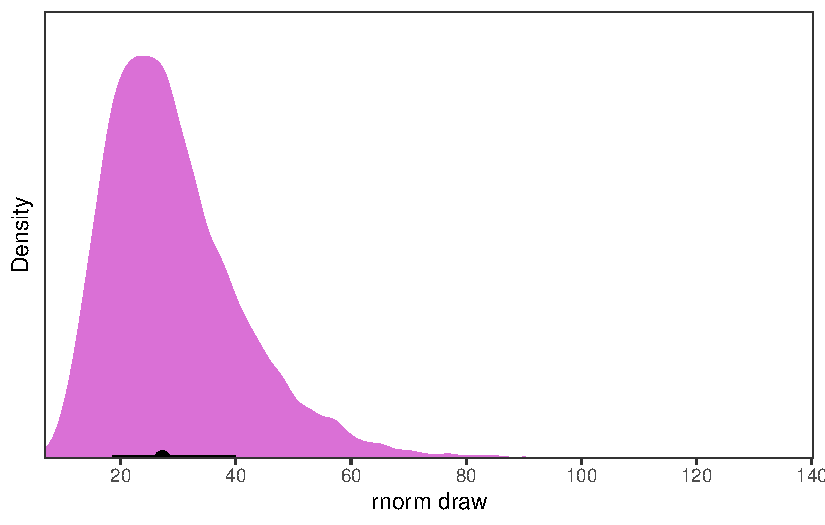
\includegraphics{./bayesian-cfa_files/figure-pdf/prior-pred-weibull-intercept-1.pdf}

}

\caption{Draws from a gaussian distribution with mean = 3.3, and sd =
.4}

\end{figure}

Now for the beta coefficients. We can think of ourselves as settings
priors as on log acceleration factors, so the exponentiated draws from
the prior should reflect our uncertainty about how a one-unit change in
that covariate might be associated with a faster or slower
time-to-employment, keeping all other measured covariates equal. For any
of the covariates, an acceleration factor of 10 or more in either
direction (I.E. 10 or 0.10) seems pretty unlikely. As with the
intercept, we fiddle with the code until we get a distribution that has
the properties we want. much trial and error it seems like a gaussian
with \texttt{mean\ =\ 0,\ sd\ =\ 1.45} captures this `factor of 5'
intuition, with a factor of 10 or greater being associated with a
probability of only about 5\% in either direction.

\begin{Shaded}
\begin{Highlighting}[]
\CommentTok{\# Simulate some data}
\NormalTok{sim }\OtherTok{\textless{}{-}} \FunctionTok{rnorm}\NormalTok{(}\DecValTok{10000}\NormalTok{, }\DecValTok{0}\NormalTok{, }\FloatTok{1.45}\NormalTok{) }\SpecialCharTok{|\textgreater{}}

  \FunctionTok{as\_tibble}\NormalTok{() }\SpecialCharTok{|\textgreater{}}

  \FunctionTok{mutate}\NormalTok{(}\AttributeTok{value =} \FunctionTok{exp}\NormalTok{(value)) }

\CommentTok{\# Get the quantiles}
\NormalTok{sim }\SpecialCharTok{|\textgreater{}} 

  \FunctionTok{summarise\_draws}\NormalTok{() }\SpecialCharTok{|\textgreater{}}

  \FunctionTok{select}\NormalTok{(q5, q95) }\SpecialCharTok{|\textgreater{}}

\NormalTok{  knitr}\SpecialCharTok{::}\FunctionTok{kable}\NormalTok{()}
\end{Highlighting}
\end{Shaded}

\begin{longtable}[]{@{}rr@{}}
\toprule()
q5 & q95 \\
\midrule()
\endhead
0.0920575 & 10.84884 \\
\bottomrule()
\end{longtable}

Exponentiated draws from a gaussian distribution with mean = 0, and sd =
1.45

\begin{Shaded}
\begin{Highlighting}[]
\CommentTok{\# Plot the distribution}
\NormalTok{sim }\SpecialCharTok{|\textgreater{}}

    \FunctionTok{ggplot}\NormalTok{(}\FunctionTok{aes}\NormalTok{(}\AttributeTok{x =}\NormalTok{ value)) }\SpecialCharTok{+}
    \FunctionTok{stat\_halfeye}\NormalTok{(}\AttributeTok{fill =} \StringTok{"orchid"}\NormalTok{) }\SpecialCharTok{+}
    \FunctionTok{scale\_x\_continuous}\NormalTok{(}\AttributeTok{limits =} \FunctionTok{c}\NormalTok{(}\DecValTok{0}\NormalTok{, }\DecValTok{30}\NormalTok{), }\AttributeTok{n.breaks =} \DecValTok{10}\NormalTok{, }\AttributeTok{expand =} \FunctionTok{c}\NormalTok{(}\DecValTok{0}\NormalTok{, }\DecValTok{0}\NormalTok{)) }\SpecialCharTok{+}
    \FunctionTok{scale\_y\_continuous}\NormalTok{(}\AttributeTok{expand =} \FunctionTok{c}\NormalTok{(}\DecValTok{0}\NormalTok{, }\DecValTok{0}\NormalTok{)) }\SpecialCharTok{+}
    \FunctionTok{labs}\NormalTok{(}
      \AttributeTok{x =} \StringTok{"rnorm draw"}\NormalTok{,}
      \AttributeTok{y =} \StringTok{"Density"}
\NormalTok{    ) }\SpecialCharTok{+}
    \FunctionTok{theme\_bw}\NormalTok{() }\SpecialCharTok{+}
    \FunctionTok{theme}\NormalTok{(}
      \AttributeTok{axis.ticks.y =} \FunctionTok{element\_blank}\NormalTok{(),}
      \AttributeTok{panel.grid.major =} \FunctionTok{element\_blank}\NormalTok{(),}
      \AttributeTok{panel.grid.minor =} \FunctionTok{element\_blank}\NormalTok{(),}
      \AttributeTok{axis.text.y =} \FunctionTok{element\_blank}\NormalTok{()}
\NormalTok{    )}
\end{Highlighting}
\end{Shaded}

\begin{figure}[H]

{\centering 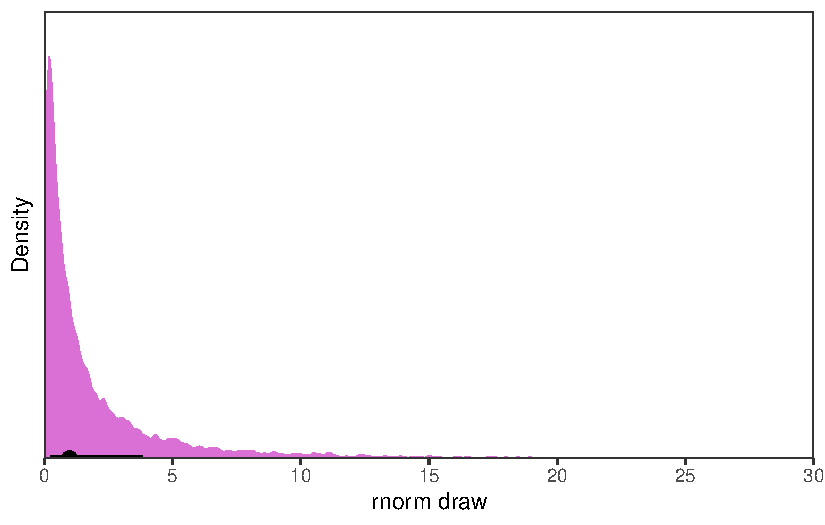
\includegraphics{./bayesian-cfa_files/figure-pdf/prior-pred-weibull-coefs-1.pdf}

}

\caption{Exponentiated draws from a gaussian distribution with mean = 0,
and sd = 1.45}

\end{figure}

Now that we have some reasonable priors, we can sample from them to
simulate from the prior predictive distribution. I don't have any
background knowledge to inform the estimate of the shape parameter, so
we can set a conventional \texttt{cauchy(0,\ 2.5)} prior to keep it
vague. The resulting densities of bounded 1-year times-to-event look
reasonable to me, and there is plenty of uncertainty leftover for the
model to refine its predictions after it sees the data.

\begin{Shaded}
\begin{Highlighting}[]
\CommentTok{\# Declare the formula}
\NormalTok{bf }\OtherTok{\textless{}{-}} \FunctionTok{formula}\NormalTok{(time }\SpecialCharTok{|} \FunctionTok{cens}\NormalTok{(censored) }\SpecialCharTok{\textasciitilde{}} \DecValTok{0} \SpecialCharTok{+}\NormalTok{ Intercept }\SpecialCharTok{+}\NormalTok{ adapt }\SpecialCharTok{+}\NormalTok{ collab }\SpecialCharTok{+}\NormalTok{ age }\SpecialCharTok{+}\NormalTok{ ei\_status)}

\CommentTok{\# See how brms names the parameters, so we know how to specify priors form them}
\FunctionTok{get\_prior}\NormalTok{(}
  \AttributeTok{formula =}\NormalTok{ bf,}
  \AttributeTok{data =}\NormalTok{ fake\_dat,}
  \AttributeTok{family =} \FunctionTok{weibull}\NormalTok{()}
\NormalTok{)}
\end{Highlighting}
\end{Shaded}

\begin{verbatim}
             prior class      coef group resp dpar nlpar lb ub       source
            (flat)     b                                            default
            (flat)     b     adapt                             (vectorized)
            (flat)     b       age                             (vectorized)
            (flat)     b    collab                             (vectorized)
            (flat)     b ei_status                             (vectorized)
            (flat)     b Intercept                             (vectorized)
 gamma(0.01, 0.01) shape                                  0         default
\end{verbatim}

\begin{Shaded}
\begin{Highlighting}[]
\CommentTok{\# Declare the priors we want}
\NormalTok{priors }\OtherTok{\textless{}{-}} \FunctionTok{c}\NormalTok{(}
    \FunctionTok{prior}\NormalTok{(}\FunctionTok{normal}\NormalTok{(}\FloatTok{3.3}\NormalTok{, .}\DecValTok{4}\NormalTok{), }\AttributeTok{class =} \StringTok{"b"}\NormalTok{, }\AttributeTok{coef =} \StringTok{"Intercept"}\NormalTok{), }\CommentTok{\# The average time{-}to{-}employment. Use gamma because times are positive and continuous}
    \FunctionTok{prior}\NormalTok{(}\FunctionTok{cauchy}\NormalTok{(}\DecValTok{0}\NormalTok{, }\FloatTok{2.5}\NormalTok{), }\AttributeTok{class =} \StringTok{"shape"}\NormalTok{), }\CommentTok{\# Constrain the shape parameter, or else it thinks event times can go on basically forever.}
    \FunctionTok{prior}\NormalTok{(}\FunctionTok{normal}\NormalTok{(}\DecValTok{0}\NormalTok{, }\FloatTok{1.45}\NormalTok{), }\AttributeTok{class =} \StringTok{"b"}\NormalTok{, }\AttributeTok{coef =} \StringTok{"adapt"}\NormalTok{),}
    \FunctionTok{prior}\NormalTok{(}\FunctionTok{normal}\NormalTok{(}\DecValTok{0}\NormalTok{, }\FloatTok{1.45}\NormalTok{), }\AttributeTok{class =} \StringTok{"b"}\NormalTok{, }\AttributeTok{coef =} \StringTok{"age"}\NormalTok{),}
    \FunctionTok{prior}\NormalTok{(}\FunctionTok{normal}\NormalTok{(}\DecValTok{0}\NormalTok{, }\FloatTok{1.45}\NormalTok{), }\AttributeTok{class =} \StringTok{"b"}\NormalTok{, }\AttributeTok{coef =} \StringTok{"collab"}\NormalTok{),}
    \FunctionTok{prior}\NormalTok{(}\FunctionTok{normal}\NormalTok{(}\DecValTok{0}\NormalTok{, }\FloatTok{1.45}\NormalTok{), }\AttributeTok{class =} \StringTok{"b"}\NormalTok{, }\AttributeTok{coef =} \StringTok{"ei\_status"}\NormalTok{)}
\NormalTok{  )}

\CommentTok{\# Fit the model}
\NormalTok{fit.prior }\OtherTok{\textless{}{-}} \FunctionTok{brm}\NormalTok{(}
  \AttributeTok{data =}\NormalTok{ fake\_dat,}
  \AttributeTok{formula =}\NormalTok{ bf,}
  \AttributeTok{family =} \FunctionTok{weibull}\NormalTok{(),}
  \AttributeTok{prior =}\NormalTok{ priors,}
  \AttributeTok{sample\_prior =} \StringTok{"only"}\NormalTok{,}
  \AttributeTok{iter =} \DecValTok{2000}\NormalTok{,}
  \AttributeTok{file =} \StringTok{"fits/b07.04.priors.rds"}
\NormalTok{)}

\CommentTok{\# Figure out what brms has named everything so we can wrangle the draws}
\CommentTok{\# get\_variables(fit.prior)}
    
\CommentTok{\# Check the prior predictive distribution}
\NormalTok{prior\_preds }\OtherTok{\textless{}{-}}\NormalTok{ fake\_dat }\SpecialCharTok{|\textgreater{}}

  \FunctionTok{add\_predicted\_draws}\NormalTok{(fit.prior, }\AttributeTok{ndraws =} \DecValTok{500}\NormalTok{) }\SpecialCharTok{|\textgreater{}}

  \FunctionTok{group\_by}\NormalTok{(rowid) }\SpecialCharTok{|\textgreater{}}

  \FunctionTok{mutate}\NormalTok{(}\AttributeTok{prior\_pred\_mean =} \FunctionTok{mean}\NormalTok{(.prediction)) }

\NormalTok{prior\_preds }\SpecialCharTok{|\textgreater{}}

  \FunctionTok{ggplot}\NormalTok{() }\SpecialCharTok{+} 
  \FunctionTok{geom\_density}\NormalTok{(}\FunctionTok{aes}\NormalTok{(}\AttributeTok{x =}\NormalTok{ .prediction, }\AttributeTok{group =}\NormalTok{ .draw), }\AttributeTok{alpha =} \DecValTok{0}\NormalTok{, }\AttributeTok{colour=}\FunctionTok{alpha}\NormalTok{(}\StringTok{"mediumorchid"}\NormalTok{, .}\DecValTok{1}\NormalTok{)) }\SpecialCharTok{+}
  \FunctionTok{scale\_y\_continuous}\NormalTok{(}\AttributeTok{expand=}\FunctionTok{c}\NormalTok{(}\DecValTok{0}\NormalTok{, }\DecValTok{0}\NormalTok{)) }\SpecialCharTok{+}
  \FunctionTok{xlim}\NormalTok{(}\FunctionTok{c}\NormalTok{(}\DecValTok{1}\NormalTok{, }\DecValTok{365}\NormalTok{)) }\SpecialCharTok{+}
  \FunctionTok{theme\_minimal}\NormalTok{() }\SpecialCharTok{+}
  \FunctionTok{theme}\NormalTok{(}
    \AttributeTok{axis.text.y =} \FunctionTok{element\_blank}\NormalTok{(),}
    \AttributeTok{axis.ticks.y =} \FunctionTok{element\_blank}\NormalTok{()}
\NormalTok{  )  }
\end{Highlighting}
\end{Shaded}

\begin{figure}[H]

{\centering 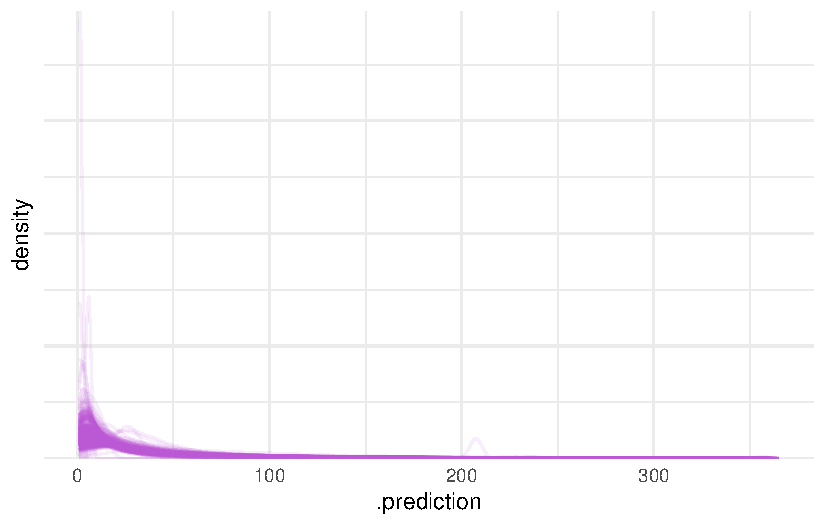
\includegraphics{./bayesian-cfa_files/figure-pdf/prior-pred-1-densities-1.pdf}

}

\caption{Densities for 500 draws from the prior predictive distribution
of event times.}

\end{figure}

We can also check the distribution of certain statistics under the prior
predictive distribution, like the mean time to event. This is something
Gelman et al. (2020) advocate in their Bayesian Workflow paper. This
reveals an area where our model seems a bit dumb: while the mode of the
means is well within our desired range of values, there is a very long
tail. This is because the Weibull distribution preserves a long tail of
event times,and we haven't told it that event times like 400,000 days
are strictly out of the question. And even though the model assigns very
tiny probability to these types of numbers, they are still there,
non-zero, pulling up the mean of the prior predictive distribution. We
can address this when we go to code the raw Stan model by specifying
better boundaries on priors and the outcome itself. Or we could give the
model this information in other ways, for example by changing the
response distribution entirely, perhaps using a 1-inflated beta
distribution to model the proportion of a year until a person found a
job, topcoding anybody who took more than a year as 1. But for now let's
stick with the plan and see if the model is able to recover the true
parameter estimates and come up with reasonable posterior predictive
distribution despite these imperfect priors.

\begin{Shaded}
\begin{Highlighting}[]
\NormalTok{fake\_dat }\SpecialCharTok{|\textgreater{}}
 
  \FunctionTok{add\_predicted\_draws}\NormalTok{(fit.prior, }\AttributeTok{ndraws =} \DecValTok{500}\NormalTok{) }\SpecialCharTok{|\textgreater{}}

  \FunctionTok{group\_by}\NormalTok{(.draw) }\SpecialCharTok{|\textgreater{}}

  \FunctionTok{mutate}\NormalTok{(}\AttributeTok{draw\_mean =} \FunctionTok{mean}\NormalTok{(.prediction)) }\SpecialCharTok{|\textgreater{}}

  \FunctionTok{distinct}\NormalTok{(.draw, }\AttributeTok{.keep\_all =} \ConstantTok{TRUE}\NormalTok{) }\SpecialCharTok{|\textgreater{}}

  \FunctionTok{ggplot}\NormalTok{() }\SpecialCharTok{+} 
  \FunctionTok{geom\_histogram}\NormalTok{(}\FunctionTok{aes}\NormalTok{(}\AttributeTok{x =}\NormalTok{ draw\_mean), }\AttributeTok{colour =} \StringTok{"white"}\NormalTok{, }\AttributeTok{fill =} \StringTok{"mediumorchid"}\NormalTok{) }\SpecialCharTok{+}
  \FunctionTok{labs}\NormalTok{(}\AttributeTok{x =} \StringTok{"Mean of draw from prior predictive distribution"}\NormalTok{, }\AttributeTok{y =} \StringTok{"n draws"}\NormalTok{) }\SpecialCharTok{+}
  \FunctionTok{scale\_x\_continuous}\NormalTok{(}\AttributeTok{expand=}\FunctionTok{c}\NormalTok{(}\DecValTok{0}\NormalTok{, }\DecValTok{0}\NormalTok{), }\AttributeTok{limits =} \FunctionTok{c}\NormalTok{(}\DecValTok{0}\NormalTok{, }\DecValTok{10000}\NormalTok{)) }\SpecialCharTok{+}
  \FunctionTok{scale\_y\_continuous}\NormalTok{(}\AttributeTok{expand=}\FunctionTok{c}\NormalTok{(}\DecValTok{0}\NormalTok{, }\DecValTok{0}\NormalTok{)) }\SpecialCharTok{+}
  \FunctionTok{theme\_minimal}\NormalTok{()}
\end{Highlighting}
\end{Shaded}

\begin{figure}[H]

{\centering 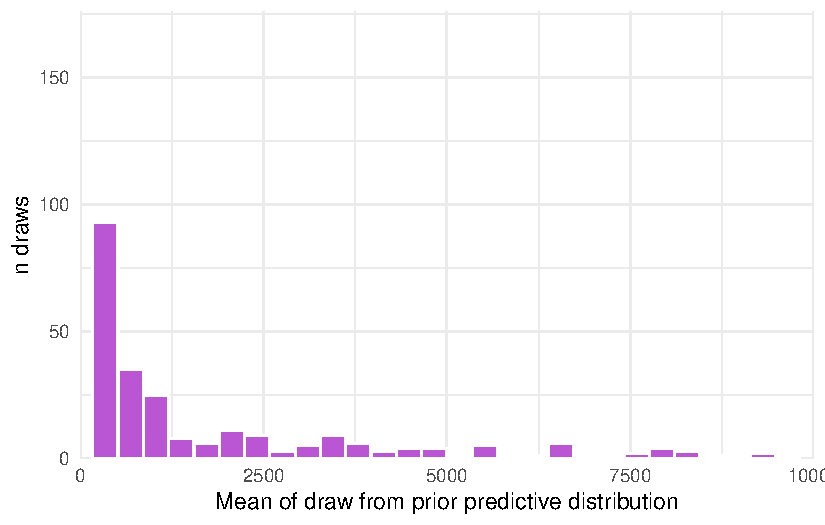
\includegraphics{./bayesian-cfa_files/figure-pdf/prior-pred-1-means-1.pdf}

}

\caption{Mean event times of 500 draws from the prior predictive
distribution of event times.}

\end{figure}

\hypertarget{fitting-the-stan-model}{%
\subsection{Fitting the Stan Model}\label{fitting-the-stan-model}}

Now we're ready to fit the survival model using the latent factors as
predictors.

\begin{Shaded}
\begin{Highlighting}[]
\KeywordTok{data}\NormalTok{ \{}
  \CommentTok{// Factor Analysis}
  \DataTypeTok{int}\NormalTok{ N; }\CommentTok{// sample size for both models}
  \DataTypeTok{int}\NormalTok{ P; }\CommentTok{// number of variables in the factor analysis}
  \DataTypeTok{int}\NormalTok{ D; }\CommentTok{// number of factors}
  \DataTypeTok{array}\NormalTok{[N] }\DataTypeTok{vector}\NormalTok{[P] X\_factor; }\CommentTok{// data matrix for factor analysis}
  \DataTypeTok{int}\NormalTok{ n\_lam; }\CommentTok{// how many factor loadings are estimated}
  
  \CommentTok{// Weibull Model}
  \DataTypeTok{vector}\NormalTok{[N] Y; }\CommentTok{// response variable for Weibull model}
  \DataTypeTok{array}\NormalTok{[N] }\DataTypeTok{int}\NormalTok{\textless{}}\KeywordTok{lower}\NormalTok{={-}}\DecValTok{1}\NormalTok{, }\KeywordTok{upper}\NormalTok{=}\DecValTok{2}\NormalTok{\textgreater{} cens; }\CommentTok{// indicates censoring for Weibull model}
  \DataTypeTok{int}\NormalTok{ K; }\CommentTok{// number of predictors in Weibull model, now it should be D + 2 + intercept}
  \DataTypeTok{matrix}\NormalTok{[N, K] X\_weibull; }\CommentTok{// population{-}level design matrix for Weibull model}
\NormalTok{\}}
\KeywordTok{parameters}\NormalTok{ \{}
  \DataTypeTok{matrix}\NormalTok{[N, D] FS\_UNC; }\CommentTok{// factor scores}
  \DataTypeTok{cholesky\_factor\_corr}\NormalTok{[D] L\_corr\_d; }\CommentTok{// cholesky correlation between factors}
  \DataTypeTok{cholesky\_factor\_corr}\NormalTok{[}\DecValTok{2}\NormalTok{] L\_corr\_m1\_m4; }\CommentTok{// cholesky correlation between the m1 and m4}
  \DataTypeTok{vector}\NormalTok{\textless{}}\KeywordTok{lower}\NormalTok{=}\DecValTok{0}\NormalTok{\textgreater{}[P] sd\_p; }\CommentTok{// residual sd for each variable in factor analysis}
  \DataTypeTok{vector}\NormalTok{\textless{}}\KeywordTok{lower}\NormalTok{={-}}\DecValTok{30}\NormalTok{, }\KeywordTok{upper}\NormalTok{=}\DecValTok{30}\NormalTok{\textgreater{}[n\_lam] lam\_UNC; }\CommentTok{// A bunch of lightly{-}constrained factor loadings}
  
  \DataTypeTok{real}\NormalTok{\textless{}}\KeywordTok{lower}\NormalTok{=}\DecValTok{0}\NormalTok{\textgreater{} shape; }\CommentTok{// shape parameter for Weibull model}
  \DataTypeTok{vector}\NormalTok{[K] b; }\CommentTok{// regression coefficients for Weibull model}
\NormalTok{\}}
\KeywordTok{transformed parameters}\NormalTok{ \{}
  \CommentTok{// Factor Analysis transformed parameters}
  \DataTypeTok{vector}\NormalTok{[D] M = rep\_vector(}\DecValTok{0}\NormalTok{, D); }\CommentTok{// factor means}
  \DataTypeTok{vector}\NormalTok{\textless{}}\KeywordTok{lower}\NormalTok{=}\DecValTok{0}\NormalTok{\textgreater{}[D] Sd\_d = rep\_vector(}\DecValTok{1}\NormalTok{, D); }\CommentTok{// factor SDs}
  \DataTypeTok{array}\NormalTok{[N] }\DataTypeTok{vector}\NormalTok{[P] mu\_UNC; }\CommentTok{// A vector to hold the linear predictors for the manifest variables}

  \ControlFlowTok{for}\NormalTok{ (i }\ControlFlowTok{in} \DecValTok{1}\NormalTok{ : N) \{}
\NormalTok{    mu\_UNC[i, }\DecValTok{1}\NormalTok{] = lam\_UNC[}\DecValTok{1}\NormalTok{] * FS\_UNC[i, }\DecValTok{1}\NormalTok{];}
\NormalTok{    mu\_UNC[i, }\DecValTok{2}\NormalTok{] = lam\_UNC[}\DecValTok{2}\NormalTok{] * FS\_UNC[i, }\DecValTok{1}\NormalTok{];}
\NormalTok{    mu\_UNC[i, }\DecValTok{3}\NormalTok{] = lam\_UNC[}\DecValTok{3}\NormalTok{] * FS\_UNC[i, }\DecValTok{1}\NormalTok{];}
\NormalTok{    mu\_UNC[i, }\DecValTok{4}\NormalTok{] = lam\_UNC[}\DecValTok{4}\NormalTok{] * FS\_UNC[i, }\DecValTok{2}\NormalTok{];}
\NormalTok{    mu\_UNC[i, }\DecValTok{5}\NormalTok{] = lam\_UNC[}\DecValTok{5}\NormalTok{] * FS\_UNC[i, }\DecValTok{2}\NormalTok{];}
\NormalTok{    mu\_UNC[i, }\DecValTok{6}\NormalTok{] = lam\_UNC[}\DecValTok{6}\NormalTok{] * FS\_UNC[i, }\DecValTok{2}\NormalTok{];}
\NormalTok{  \}}
  
  \DataTypeTok{cholesky\_factor\_cov}\NormalTok{[D] L\_Sigma = diag\_pre\_multiply(Sd\_d, L\_corr\_d); }\CommentTok{// var{-}covar matrix for the factors}
  \DataTypeTok{cholesky\_factor\_cov}\NormalTok{[D] L\_Sigma\_m1\_m4 = diag\_pre\_multiply(sd\_p[\{}\DecValTok{1}\NormalTok{, }\DecValTok{4}\NormalTok{\}], L\_corr\_m1\_m4); }\CommentTok{// var{-}covar matrix of m1 and m4}
  
  \CommentTok{// Weibull transformed parameters}
  \DataTypeTok{vector}\NormalTok{[N] mu\_weibull = rep\_vector(}\FloatTok{0.0}\NormalTok{, N); }\CommentTok{// initialize linear predictor term for Weibull model}
\NormalTok{  mu\_weibull += X\_weibull * b; }\CommentTok{// use both factor scores and observed predictors as predictors}
\NormalTok{\}}
\KeywordTok{model}\NormalTok{ \{}
  \CommentTok{// Factor Analysis}
\NormalTok{  L\_corr\_d \textasciitilde{} lkj\_corr\_cholesky(}\DecValTok{1}\NormalTok{);}
\NormalTok{  L\_corr\_m1\_m4 \textasciitilde{} lkj\_corr\_cholesky(}\DecValTok{1}\NormalTok{);}
\NormalTok{  lam\_UNC \textasciitilde{} normal(}\DecValTok{0}\NormalTok{, }\DecValTok{10}\NormalTok{);}
\NormalTok{  sd\_p \textasciitilde{} cauchy(}\DecValTok{0}\NormalTok{, }\FloatTok{2.5}\NormalTok{);}
  
  \ControlFlowTok{for}\NormalTok{ (i }\ControlFlowTok{in} \DecValTok{1}\NormalTok{ : N) \{}
    \ControlFlowTok{for}\NormalTok{ (j }\ControlFlowTok{in}\NormalTok{ \{}\DecValTok{2}\NormalTok{,}\DecValTok{3}\NormalTok{,}\DecValTok{5}\NormalTok{,}\DecValTok{6}\NormalTok{\}) \{}
\NormalTok{      X\_factor[i, j] \textasciitilde{} normal(mu\_UNC[i, j], sd\_p[j]);}
\NormalTok{    \}}
\NormalTok{    to\_vector(\{X\_factor[i, }\DecValTok{1}\NormalTok{], X\_factor[i, }\DecValTok{4}\NormalTok{]\}) \textasciitilde{} multi\_normal\_cholesky([mu\_UNC[i, }\DecValTok{1}\NormalTok{], mu\_UNC[i, }\DecValTok{4}\NormalTok{]]\textquotesingle{}, L\_Sigma\_m1\_m4);}
\NormalTok{    FS\_UNC[i] \textasciitilde{} multi\_normal\_cholesky(M, L\_Sigma);}
\NormalTok{  \}}

  \CommentTok{// Weibull Survival Analysis}
\NormalTok{  shape \textasciitilde{} cauchy(}\DecValTok{0}\NormalTok{, }\FloatTok{2.5}\NormalTok{);}
\NormalTok{  b[}\DecValTok{1}\NormalTok{] \textasciitilde{} normal(}\FloatTok{3.3}\NormalTok{, }\FloatTok{0.4}\NormalTok{);}
  \ControlFlowTok{for}\NormalTok{ (k }\ControlFlowTok{in} \DecValTok{2}\NormalTok{:K) \{}
\NormalTok{    b[k] \textasciitilde{} normal(}\DecValTok{0}\NormalTok{, }\FloatTok{1.45}\NormalTok{);}
\NormalTok{  \}}
  \ControlFlowTok{for}\NormalTok{ (n }\ControlFlowTok{in} \DecValTok{1}\NormalTok{ : N) \{}
    \ControlFlowTok{if}\NormalTok{ (cens[n] == }\DecValTok{0}\NormalTok{) \{}
      \KeywordTok{target +=}\NormalTok{ weibull\_lpdf(Y[n] | shape, exp(mu\_weibull[n]) / tgamma(}\DecValTok{1}\NormalTok{ + }\DecValTok{1}\NormalTok{ / shape));}
\NormalTok{    \} }\ControlFlowTok{else} \ControlFlowTok{if}\NormalTok{ (cens[n] == }\DecValTok{1}\NormalTok{) \{}
      \KeywordTok{target +=}\NormalTok{ weibull\_lccdf(Y[n] | shape, exp(mu\_weibull[n]) / tgamma(}\DecValTok{1}\NormalTok{ + }\DecValTok{1}\NormalTok{ / shape));}
\NormalTok{    \} }
\NormalTok{  \}}
\NormalTok{\}}
\KeywordTok{generated quantities}\NormalTok{ \{}
  \DataTypeTok{corr\_matrix}\NormalTok{[D] Rho\_UNC; }\CommentTok{// correlation matrix for factors}
  \DataTypeTok{corr\_matrix}\NormalTok{[D] Rho\_factors; }\CommentTok{// correlation matrix for factors}
  \DataTypeTok{corr\_matrix}\NormalTok{[D] Rho\_m1\_m4; }\CommentTok{// correlation matrix for m1 and m4}
  \DataTypeTok{matrix}\NormalTok{[P, D] lam; }\CommentTok{// factor loadings}
  \DataTypeTok{matrix}\NormalTok{[N, D] FS; }\CommentTok{// factor scores}
  
\NormalTok{  Rho\_UNC = multiply\_lower\_tri\_self\_transpose(L\_corr\_d);}
\NormalTok{  Rho\_factors = Rho\_UNC;}
\NormalTok{  Rho\_m1\_m4 = multiply\_lower\_tri\_self\_transpose(L\_corr\_m1\_m4);}
\NormalTok{  FS = FS\_UNC;}
\NormalTok{  lam = rep\_matrix(}\DecValTok{0}\NormalTok{, P, D);}
\NormalTok{  lam[}\DecValTok{1}\NormalTok{ : }\DecValTok{3}\NormalTok{, }\DecValTok{1}\NormalTok{] = to\_vector(lam\_UNC[}\DecValTok{1}\NormalTok{ : }\DecValTok{3}\NormalTok{]);}
\NormalTok{  lam[}\DecValTok{4}\NormalTok{ : }\DecValTok{6}\NormalTok{, }\DecValTok{2}\NormalTok{] = to\_vector(lam\_UNC[}\DecValTok{4}\NormalTok{ : }\DecValTok{6}\NormalTok{]);}
  
  \ControlFlowTok{if}\NormalTok{ (lam\_UNC[}\DecValTok{1}\NormalTok{] \textless{} }\DecValTok{0}\NormalTok{) \{}
\NormalTok{    lam[}\DecValTok{1}\NormalTok{ : }\DecValTok{3}\NormalTok{, }\DecValTok{1}\NormalTok{] = to\_vector({-}}\DecValTok{1}\NormalTok{ * lam\_UNC[}\DecValTok{1}\NormalTok{ : }\DecValTok{3}\NormalTok{]);}
\NormalTok{    FS[ : , }\DecValTok{1}\NormalTok{] = to\_vector({-}}\DecValTok{1}\NormalTok{ * FS\_UNC[ : , }\DecValTok{1}\NormalTok{]);}
    \ControlFlowTok{if}\NormalTok{ (lam\_UNC[}\DecValTok{4}\NormalTok{] \textgreater{} }\DecValTok{0}\NormalTok{) \{}
\NormalTok{      Rho\_factors[}\DecValTok{1}\NormalTok{, }\DecValTok{2}\NormalTok{] = {-}}\DecValTok{1}\NormalTok{ * Rho\_UNC[}\DecValTok{1}\NormalTok{, }\DecValTok{2}\NormalTok{];}
\NormalTok{      Rho\_factors[}\DecValTok{2}\NormalTok{, }\DecValTok{1}\NormalTok{] = {-}}\DecValTok{1}\NormalTok{ * Rho\_UNC[}\DecValTok{2}\NormalTok{, }\DecValTok{1}\NormalTok{];}
\NormalTok{    \}}
\NormalTok{  \}}
  \ControlFlowTok{if}\NormalTok{ (lam\_UNC[}\DecValTok{4}\NormalTok{] \textless{} }\DecValTok{0}\NormalTok{) \{}
\NormalTok{    lam[}\DecValTok{4}\NormalTok{ : }\DecValTok{6}\NormalTok{, }\DecValTok{2}\NormalTok{] = to\_vector({-}}\DecValTok{1}\NormalTok{ * lam\_UNC[}\DecValTok{4}\NormalTok{ : }\DecValTok{6}\NormalTok{]);}
\NormalTok{    FS[ : , }\DecValTok{2}\NormalTok{] = to\_vector({-}}\DecValTok{1}\NormalTok{ * FS\_UNC[ : , }\DecValTok{2}\NormalTok{]);}
    \ControlFlowTok{if}\NormalTok{ (lam\_UNC[}\DecValTok{1}\NormalTok{] \textgreater{} }\DecValTok{0}\NormalTok{) \{}
\NormalTok{      Rho\_factors[}\DecValTok{2}\NormalTok{, }\DecValTok{1}\NormalTok{] = {-}}\DecValTok{1}\NormalTok{ * Rho\_UNC[}\DecValTok{2}\NormalTok{, }\DecValTok{1}\NormalTok{];}
\NormalTok{      Rho\_factors[}\DecValTok{1}\NormalTok{, }\DecValTok{2}\NormalTok{] = {-}}\DecValTok{1}\NormalTok{ * Rho\_UNC[}\DecValTok{1}\NormalTok{, }\DecValTok{2}\NormalTok{];}
\NormalTok{    \}}
\NormalTok{  \}}

  \CommentTok{// Draws from posterior predictive distribution}
  \DataTypeTok{vector}\NormalTok{[N] y\_pred;}
  \ControlFlowTok{for}\NormalTok{ (n }\ControlFlowTok{in} \DecValTok{1}\NormalTok{:N) \{}
\NormalTok{    y\_pred[n] = weibull\_rng(shape, exp(mu\_weibull[n]) / tgamma(}\DecValTok{1}\NormalTok{ + }\DecValTok{1}\NormalTok{ / shape));}
\NormalTok{  \}}
\NormalTok{\}}
\end{Highlighting}
\end{Shaded}

Now compline the model and run. I've worked closely from the Stan code
for the Weibull model we fit with \textbf{brms} above, essentially just
grafting it onto the MTMM factor analysis model from before. This only
involved a few steps:

\begin{itemize}
\tightlist
\item
  \textbf{Data block:} add new vectors for the response variable
  \texttt{Y} and predictor variables \texttt{K} of the Weibull model,
  and for censoring status \texttt{cens}. Also declare the design matrix
  \texttt{X\_weibull} of the necessary dimensions.
\item
  \textbf{Parameters block:} add a vector of coefficients \texttt{b} for
  the beta coefficients of the Weibull model.
\item
  \textbf{Transformed Parameters block:} declare the constant shape
  parameter for the Weibull model, as well as the linear predictor
  \texttt{mu} for each observation. Then exponentiate it.
\item
  \textbf{Model block:} add the priors we simulated above, as well as
  the likelihood function conditional on censoring status.
\item
  \textbf{Generated Quantities block:} generate draws from the posterior
  predictive distribution, to help with model checking.
\end{itemize}

One thing to note is that because we adopted \textbf{brms}'s
\texttt{0\ +\ Intercept} syntax in generating the Stan code to allow us
to set the intercept prior on the raw outcome scale, we can do what Paul
Bürkner does under the hood and feed an extra column of 1s into the
design matrix \texttt{X\_weibull}.

\begin{Shaded}
\begin{Highlighting}[]
\CommentTok{\# Write the raw Stan code from an R string to a Stan file}
\NormalTok{stan\_file }\OtherTok{\textless{}{-}}\NormalTok{ cmdstanr}\SpecialCharTok{::}\FunctionTok{write\_stan\_file}\NormalTok{(stan\_model\_code)}

\CommentTok{\# Autoformat the model syntax to preempt any warnings at compile time}
\NormalTok{model }\OtherTok{\textless{}{-}}\NormalTok{ cmdstanr}\SpecialCharTok{::}\FunctionTok{cmdstan\_model}\NormalTok{(stan\_file, }\AttributeTok{compile =} \ConstantTok{FALSE}\NormalTok{)}
\NormalTok{model}\SpecialCharTok{$}\FunctionTok{format}\NormalTok{(}\AttributeTok{canonicalize =} \ConstantTok{TRUE}\NormalTok{)}

\CommentTok{\# Compile the model from the Stan file}
\NormalTok{model }\OtherTok{\textless{}{-}}\NormalTok{ cmdstanr}\SpecialCharTok{::}\FunctionTok{cmdstan\_model}\NormalTok{(stan\_file)}

\CommentTok{\# Put the data into a list format Stan can understand}
\NormalTok{P }\OtherTok{\textless{}{-}} \DecValTok{8} \CommentTok{\# Because 6 measured variables + 2 factors }
\NormalTok{N }\OtherTok{\textless{}{-}} \FunctionTok{nrow}\NormalTok{(fake\_dat)}
\NormalTok{D }\OtherTok{\textless{}{-}} \DecValTok{2}
\NormalTok{X\_factor }\OtherTok{\textless{}{-}} \FunctionTok{as.matrix}\NormalTok{(fake\_dat }\SpecialCharTok{|\textgreater{}} \FunctionTok{select}\NormalTok{(}\FunctionTok{matches}\NormalTok{(}\StringTok{"\^{}m[1{-}9]$|\^{}adapt$|\^{}collab$"}\NormalTok{)))}

\NormalTok{Y }\OtherTok{\textless{}{-}}\NormalTok{ fake\_dat}\SpecialCharTok{$}\NormalTok{time}
\NormalTok{cens }\OtherTok{\textless{}{-}}\NormalTok{ fake\_dat}\SpecialCharTok{$}\NormalTok{censored}
\NormalTok{X\_weibull }\OtherTok{\textless{}{-}} \FunctionTok{as.matrix}\NormalTok{(}
\NormalTok{  fake\_dat }\SpecialCharTok{|\textgreater{}} 
    \FunctionTok{mutate}\NormalTok{(}\AttributeTok{intercept =} \DecValTok{1}\NormalTok{) }\SpecialCharTok{|\textgreater{}}
    \FunctionTok{select}\NormalTok{(}
\NormalTok{      intercept,}
\NormalTok{      adapt,}
\NormalTok{      collab,}
\NormalTok{      age,}
\NormalTok{      ei\_status}
\NormalTok{    ) }
\NormalTok{)}

\NormalTok{data\_list }\OtherTok{\textless{}{-}} \FunctionTok{list}\NormalTok{(}
  \AttributeTok{N=}\NormalTok{N,}
  \AttributeTok{P=}\NormalTok{P,}
  \AttributeTok{D=}\NormalTok{D,}
  \AttributeTok{X\_factor=}\NormalTok{X\_factor, }
  \AttributeTok{n\_lam=}\DecValTok{6}\NormalTok{,}
  \AttributeTok{Y=}\NormalTok{Y,}
  \AttributeTok{K=}\DecValTok{5}\NormalTok{, }\CommentTok{\# four predictors plus a dummy column of 1s for the intercept}
  \AttributeTok{cens=}\NormalTok{cens,}
  \AttributeTok{X\_weibull=}\NormalTok{X\_weibull}
\NormalTok{)}

\CommentTok{\# Fit the model}
\NormalTok{fit }\OtherTok{\textless{}{-}}\NormalTok{ model}\SpecialCharTok{$}\FunctionTok{sample}\NormalTok{(}
  \AttributeTok{data =}\NormalTok{ data\_list,}
  \AttributeTok{seed =} \DecValTok{199}\NormalTok{,}
  \AttributeTok{chains =} \DecValTok{4}\NormalTok{,}
  \AttributeTok{parallel\_chains =} \DecValTok{4}\NormalTok{,}
  \AttributeTok{iter\_warmup =} \DecValTok{1000}\NormalTok{,}
  \AttributeTok{iter\_sampling =} \DecValTok{6000}\NormalTok{,}
  \AttributeTok{output\_dir =} \StringTok{"fits"}\NormalTok{,}
  \AttributeTok{refresh =} \DecValTok{1} \CommentTok{\# print update at each iter}
\NormalTok{)}


\CommentTok{\# Save the resulting model fit}
\FunctionTok{saveRDS}\NormalTok{(fit, }\StringTok{"fits/b07.04.rds"}\NormalTok{)}
\end{Highlighting}
\end{Shaded}

\begin{Shaded}
\begin{Highlighting}[]
\NormalTok{fit }\OtherTok{\textless{}{-}} \FunctionTok{readRDS}\NormalTok{(}\StringTok{"fits/b07.04.rds"}\NormalTok{)}

\CommentTok{\# If you need to check variable names, call this and inspect the resulting object}
\CommentTok{\#summary \textless{}{-} fit$summary()}

\CommentTok{\# Load the MCMC draws from the variables we care about}
\NormalTok{draws }\OtherTok{\textless{}{-}}\NormalTok{ fit}\SpecialCharTok{$}\FunctionTok{draws}\NormalTok{(}
  \AttributeTok{variables =} \FunctionTok{c}\NormalTok{(}
  \StringTok{"lam[1,1]"}\NormalTok{,}
  \StringTok{"lam[2,1]"}\NormalTok{,}
  \StringTok{"lam[3,1]"}\NormalTok{,}
  \StringTok{"lam[4,2]"}\NormalTok{,}
  \StringTok{"lam[5,2]"}\NormalTok{,}
  \StringTok{"lam[6,2]"}\NormalTok{,}
  \StringTok{"Rho\_factors[2,1]"}\NormalTok{, }
  \StringTok{"Rho\_m1\_m4[2,1]"}\NormalTok{,}
  \StringTok{"b"}
\NormalTok{  )}
\NormalTok{)}

\NormalTok{pp\_draws }\OtherTok{\textless{}{-}}\NormalTok{ fit}\SpecialCharTok{$}\FunctionTok{draws}\NormalTok{(}
  \AttributeTok{variables =} \FunctionTok{c}\NormalTok{(}
    \StringTok{"y\_pred"}
\NormalTok{  )}
\NormalTok{)}
\CommentTok{\# Save the result}
\FunctionTok{saveRDS}\NormalTok{(draws, }\StringTok{"fits/b07.04.samples.rds"}\NormalTok{)}
\FunctionTok{saveRDS}\NormalTok{(pp\_draws, }\StringTok{"fits/b07.04.post\_pred\_samples.rds"}\NormalTok{)}
\end{Highlighting}
\end{Shaded}

How did that go? We can plot the draws and look at the MCMC diagnostics
like we did above. It looks like the model did a good job capturing all
of the true parameter estimates in the form of acceleration factors. For
example, where we simulated our true parameter value for the effect of a
1-year It even did ok at recovering the true parameter estimates for
\texttt{b\_Collab}, even though the simulated factor loadings provide
quite unreliable measurements of that latent predictor. This is all a
big win for Bayes.

\begin{Shaded}
\begin{Highlighting}[]
\CommentTok{\# Load the draws saved in the previous block}
\NormalTok{draws }\OtherTok{\textless{}{-}} \FunctionTok{readRDS}\NormalTok{(}\StringTok{"fits/b07.04.samples.rds"}\NormalTok{)}

\CommentTok{\# Plot}
\NormalTok{draws }\SpecialCharTok{|\textgreater{}}

  \CommentTok{\# Get the raw draws for the factor loadings and the beween{-}factor correlation coefficient}
  \FunctionTok{gather\_draws}\NormalTok{(}
    \StringTok{\textasciigrave{}}\AttributeTok{b[1]}\StringTok{\textasciigrave{}}\NormalTok{,}
    \StringTok{\textasciigrave{}}\AttributeTok{b[2]}\StringTok{\textasciigrave{}}\NormalTok{,}
    \StringTok{\textasciigrave{}}\AttributeTok{b[3]}\StringTok{\textasciigrave{}}\NormalTok{,}
    \StringTok{\textasciigrave{}}\AttributeTok{b[4]}\StringTok{\textasciigrave{}}\NormalTok{,}
    \StringTok{\textasciigrave{}}\AttributeTok{b[5]}\StringTok{\textasciigrave{}}\NormalTok{,}
    \StringTok{\textasciigrave{}}\AttributeTok{lam[1,1]}\StringTok{\textasciigrave{}}\NormalTok{,}
    \StringTok{\textasciigrave{}}\AttributeTok{lam[2,1]}\StringTok{\textasciigrave{}}\NormalTok{,}
    \StringTok{\textasciigrave{}}\AttributeTok{lam[3,1]}\StringTok{\textasciigrave{}}\NormalTok{,}
    \StringTok{\textasciigrave{}}\AttributeTok{lam[4,2]}\StringTok{\textasciigrave{}}\NormalTok{,}
    \StringTok{\textasciigrave{}}\AttributeTok{lam[5,2]}\StringTok{\textasciigrave{}}\NormalTok{,}
    \StringTok{\textasciigrave{}}\AttributeTok{lam[6,2]}\StringTok{\textasciigrave{}}\NormalTok{,}
    \StringTok{\textasciigrave{}}\AttributeTok{Rho\_factors[2,1]}\StringTok{\textasciigrave{}}\NormalTok{,}
    \StringTok{\textasciigrave{}}\AttributeTok{Rho\_m1\_m4[2,1]}\StringTok{\textasciigrave{}}
\NormalTok{  ) }\SpecialCharTok{|\textgreater{}}

  \FunctionTok{mutate}\NormalTok{(}\AttributeTok{.value =} \FunctionTok{ifelse}\NormalTok{(.variable }\SpecialCharTok{\%in\%} \FunctionTok{c}\NormalTok{(}\StringTok{"b[1]"}\NormalTok{, }\StringTok{"b[2]"}\NormalTok{, }\StringTok{"b[3]"}\NormalTok{, }\StringTok{"b[4]"}\NormalTok{, }\StringTok{"b[5]"}\NormalTok{), }\FunctionTok{exp}\NormalTok{(.value), .value)) }\SpecialCharTok{|\textgreater{}}
  
  \CommentTok{\# Do some renaming for clarity}
  \FunctionTok{mutate}\NormalTok{(}\AttributeTok{.variable =} \FunctionTok{case\_when}\NormalTok{(}
\NormalTok{   .variable }\SpecialCharTok{==} \StringTok{"b[1]"} \SpecialCharTok{\textasciitilde{}} \StringTok{"Intercept"}\NormalTok{,}
\NormalTok{   .variable }\SpecialCharTok{==} \StringTok{"b[2]"} \SpecialCharTok{\textasciitilde{}} \StringTok{"b\_Adapt"}\NormalTok{,}
\NormalTok{   .variable }\SpecialCharTok{==} \StringTok{"b[3]"} \SpecialCharTok{\textasciitilde{}} \StringTok{"b\_Collab"}\NormalTok{,}
\NormalTok{   .variable }\SpecialCharTok{==} \StringTok{"b[4]"} \SpecialCharTok{\textasciitilde{}} \StringTok{"b\_Age"}\NormalTok{,}
\NormalTok{   .variable }\SpecialCharTok{==} \StringTok{"b[5]"} \SpecialCharTok{\textasciitilde{}} \StringTok{"b\_EI Status"}\NormalTok{,}
\NormalTok{   .variable }\SpecialCharTok{==} \StringTok{"lam[1,1]"} \SpecialCharTok{\textasciitilde{}} \StringTok{"Loading for m1"}\NormalTok{,}
\NormalTok{   .variable }\SpecialCharTok{==} \StringTok{"lam[2,1]"} \SpecialCharTok{\textasciitilde{}} \StringTok{"Loading for m2"}\NormalTok{,}
\NormalTok{   .variable }\SpecialCharTok{==} \StringTok{"lam[3,1]"} \SpecialCharTok{\textasciitilde{}} \StringTok{"Loading for m3"}\NormalTok{,}
\NormalTok{   .variable }\SpecialCharTok{==} \StringTok{"lam[4,2]"} \SpecialCharTok{\textasciitilde{}} \StringTok{"Loading for m4"}\NormalTok{,}
\NormalTok{   .variable }\SpecialCharTok{==} \StringTok{"lam[5,2]"} \SpecialCharTok{\textasciitilde{}} \StringTok{"Loading for m5"}\NormalTok{,}
\NormalTok{   .variable }\SpecialCharTok{==} \StringTok{"lam[6,2]"} \SpecialCharTok{\textasciitilde{}} \StringTok{"Loading for m6"}\NormalTok{,}
\NormalTok{   .variable }\SpecialCharTok{==} \StringTok{"Rho\_factors[2,1]"} \SpecialCharTok{\textasciitilde{}} \StringTok{"Covariance for f1 \textasciitilde{} f2"}\NormalTok{,}
\NormalTok{   .variable }\SpecialCharTok{==} \StringTok{"Rho\_m1\_m4[2,1]"} \SpecialCharTok{\textasciitilde{}} \StringTok{"Covariance for m1 \textasciitilde{} m4"}
\NormalTok{ )) }\SpecialCharTok{|\textgreater{}}

  \FunctionTok{filter}\NormalTok{(.variable }\SpecialCharTok{!=} \StringTok{"Intercept"}\NormalTok{) }\SpecialCharTok{|\textgreater{}}

  \CommentTok{\# Add the true factor loadings for plotting}
  \FunctionTok{mutate}\NormalTok{(}\AttributeTok{true\_loading =} \FunctionTok{case\_when}\NormalTok{(}
\NormalTok{    .variable }\SpecialCharTok{==} \StringTok{"b\_Age"} \SpecialCharTok{\textasciitilde{}} \FloatTok{1.11}\NormalTok{,}
\NormalTok{    .variable }\SpecialCharTok{==} \StringTok{"b\_Collab"} \SpecialCharTok{\textasciitilde{}} \FloatTok{0.833}\NormalTok{,}
\NormalTok{    .variable }\SpecialCharTok{==} \StringTok{"b\_Adapt"} \SpecialCharTok{\textasciitilde{}} \DecValTok{1}\NormalTok{,}
\NormalTok{    .variable }\SpecialCharTok{==} \StringTok{"b\_EI Status"} \SpecialCharTok{\textasciitilde{}} \FloatTok{0.5}\NormalTok{,}
\NormalTok{    .variable }\SpecialCharTok{==} \StringTok{"Loading for m1"} \SpecialCharTok{\textasciitilde{}}\NormalTok{ .}\DecValTok{8}\NormalTok{,}
\NormalTok{    .variable }\SpecialCharTok{==} \StringTok{"Loading for m2"} \SpecialCharTok{\textasciitilde{}}\NormalTok{ .}\DecValTok{6}\NormalTok{,}
\NormalTok{    .variable }\SpecialCharTok{==} \StringTok{"Loading for m3"} \SpecialCharTok{\textasciitilde{}}\NormalTok{ .}\DecValTok{9}\NormalTok{,}
\NormalTok{    .variable }\SpecialCharTok{==} \StringTok{"Loading for m4"} \SpecialCharTok{\textasciitilde{}}\NormalTok{ .}\DecValTok{1}\NormalTok{,}
\NormalTok{    .variable }\SpecialCharTok{==} \StringTok{"Loading for m5"} \SpecialCharTok{\textasciitilde{}}\NormalTok{ .}\DecValTok{2}\NormalTok{,}
\NormalTok{    .variable }\SpecialCharTok{==} \StringTok{"Loading for m6"} \SpecialCharTok{\textasciitilde{}} \SpecialCharTok{{-}}\NormalTok{.}\DecValTok{4}\NormalTok{,}
\NormalTok{    .variable }\SpecialCharTok{==} \StringTok{"Covariance for f1 \textasciitilde{} f2"} \SpecialCharTok{\textasciitilde{}}\NormalTok{ .}\DecValTok{4}\NormalTok{,}
\NormalTok{    .variable }\SpecialCharTok{==} \StringTok{"Covariance for m1 \textasciitilde{} m4"} \SpecialCharTok{\textasciitilde{}}\NormalTok{ .}\DecValTok{4}
\NormalTok{  )) }\SpecialCharTok{|\textgreater{}}

  \FunctionTok{ggplot}\NormalTok{(}\FunctionTok{aes}\NormalTok{(}\AttributeTok{x =}\NormalTok{ .value, }\AttributeTok{fill =}\NormalTok{ .variable)) }\SpecialCharTok{+}
  \FunctionTok{stat\_halfeye}\NormalTok{(}\AttributeTok{fill =} \StringTok{"mediumorchid"}\NormalTok{) }\SpecialCharTok{+}
  \FunctionTok{geom\_vline}\NormalTok{(}\FunctionTok{aes}\NormalTok{(}\AttributeTok{xintercept =}\NormalTok{ true\_loading), }\AttributeTok{linetype =} \DecValTok{2}\NormalTok{) }\SpecialCharTok{+} 
  \FunctionTok{scale\_x\_continuous}\NormalTok{(}\AttributeTok{expand =} \FunctionTok{c}\NormalTok{(}\DecValTok{0}\NormalTok{, }\FloatTok{0.015}\NormalTok{)) }\SpecialCharTok{+}
  \FunctionTok{scale\_y\_continuous}\NormalTok{(}\AttributeTok{expand =} \FunctionTok{c}\NormalTok{(}\DecValTok{0}\NormalTok{, }\FloatTok{0.015}\NormalTok{)) }\SpecialCharTok{+}
  \FunctionTok{guides}\NormalTok{(}\AttributeTok{fill =} \StringTok{"none"}\NormalTok{) }\SpecialCharTok{+}
  \FunctionTok{labs}\NormalTok{(}\AttributeTok{x =} \StringTok{"lab"}\NormalTok{,}
     \AttributeTok{y =} \ConstantTok{NULL}\NormalTok{)  }\SpecialCharTok{+}
  \FunctionTok{theme\_minimal}\NormalTok{() }\SpecialCharTok{+} 
  \FunctionTok{theme}\NormalTok{(}\AttributeTok{panel.grid.major =} \FunctionTok{element\_blank}\NormalTok{()) }\SpecialCharTok{+}
  \FunctionTok{facet\_wrap}\NormalTok{(}\SpecialCharTok{\textasciitilde{}}\NormalTok{.variable, }\AttributeTok{scales =} \StringTok{"free\_x"}\NormalTok{) }
\end{Highlighting}
\end{Shaded}

\begin{figure}[H]

{\centering 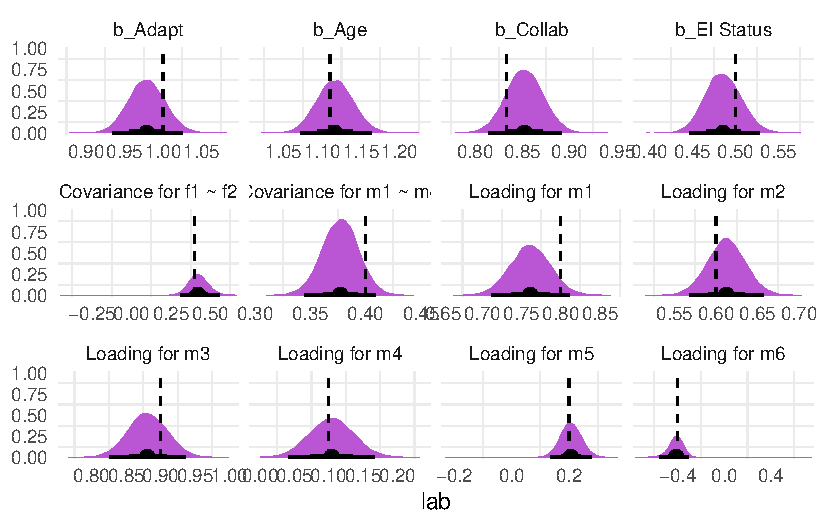
\includegraphics{./bayesian-cfa_files/figure-pdf/unnamed-chunk-37-1.pdf}

}

\end{figure}

Bring the posterior checks code and saveRDS call down here for
consistency.

Plot baseline hazard, etc, other conventional time-to-event model
diagnostics.

\hypertarget{multilevel-survival-analysis}{%
\section{Multilevel Survival
Analysis}\label{multilevel-survival-analysis}}

Let's say like 30 clusters. How to simulate? Vary cluster N to
illustrate shrinkage in posterior predictions.

Do a secret weapon plot for the cluster-specific estimates before
fitting the full model!

\part{Structural Equation Modelling}

Someone on the stan forums recommended this book for a bayesian example:
https://www.guilford.com/books/Bayesian-Structural-Equation-Modeling/Sarah-Depaoli/9781462547746

\hypertarget{example-survival-analysis-with-latent-variables}{%
\chapter{Example: Survival Analysis with Latent
Variables}\label{example-survival-analysis-with-latent-variables}}

The line between SEM and classic regression starts to blur when we
realize we can mix-and-match latent and observed variables in a
regression, defining whichever relationships make the most sense given
our background knowledge.

A traditional way of incorporating a CFA measurement model into a fuller
regression analysis proceeds in two steps:

\begin{enumerate}
\def\labelenumi{\arabic{enumi}.}
\tightlist
\item
  first you fit the CFA model,
\item
  then you fit the substantive regression, incorporating the latent
  variable into the regression by generating factor scores from the CFA
  model for each observation and including those as a regression
  covariate.
\end{enumerate}

But this approach is unsatisfactory because factor scores are a function
of the CFA model's parameter estimates (the estimates of the factor
loadings), about which there is uncertainty. So if we only give our
substantive regression model a point-estimate factor score from the CFA
model, we ignore the uncertainty contained in the standard errors of the
CFA model's factor loading estimates. This is the approach taken by
Kankaraš, Feron, and Renbarger (2019); they use point-estimate factor
scores as predictors in subsequent regressions. In some cases they even
do this iteratively, fitting measurement models on point-estimate factor
scores from measurement models fit on point-estimate factor scores, and
using \emph{those} point-estimates as regression predictors! In their
analysis they don't even report the standard errors of the factor
loadings from their measurement models.

A better option is to fit a Bayesian model that carries out both the
measurement model and the substantive regression model simultaneously,
so that the model can incorporate its uncertainty from the CFA model
into its substantive parameter estimates and predictions. This section
provides an example of how to implement just such a Bayesian model in a
survival analysis context in STAN via the \textbf{brms} R package.

\hypertarget{background-and-data-simulation}{%
\section{Background and Data
Simulation}\label{background-and-data-simulation}}

\begin{Shaded}
\begin{Highlighting}[]
\FunctionTok{library}\NormalTok{(tidyverse)}
\FunctionTok{library}\NormalTok{(lavaan)}
\FunctionTok{library}\NormalTok{(ordinal)}
\end{Highlighting}
\end{Shaded}

For this example we'll simulate some data related to the subject matter
of Kankaraš, Feron, and Renbarger (2019). Specifically, we'll simulate
some data in which latent social and emotional skills predict
time-to-employment to varying degrees. More specifically, here is what
the dataset should contain:

\begin{enumerate}
\def\labelenumi{\arabic{enumi}.}
\tightlist
\item
  n participants in a skills training program;
\item
  Some continuous and categorical demographic variables for each
  participant, such as age, gender priority group (this should be
  TRUE/FALSE), barriers to employment, and n previous services accessed.
\item
  a latent variable called `communication' with an arbitrary scale of
  0-100.
\item
  a scale of 5 measurements each for this latent variable, each on a
  likert scale from 1-5. These should each be a function of the
  corresponding latent variable plus noise, where the degree of
  correlation should be controllable by the user via function arguments.
\item
  the outcome variable, time, which should be a function of the latent
  variables and the demographhic variables and noise
\item
  a status variable indicating whether time refers to time-to-employment
  or time-to-censoring. This should be random for non-informative
  censoring, with the probability of censoring being controllable by the
  user.
\end{enumerate}

For now we'll assume the latent variables are not correlated, even
though this is a bit of a silly assumption in practice.

One improvement we can make on the traitional factor analyses we looked
at in previous sections is that we can specify our measurement model
with ordinal relationships between the factor and its measurements. This
makes sense given that the measurements are likert, andd it doesn't make
sense to assume likert variables move linearly.

It would be most efficient to just define a function that creates the
dataset we need based on various parameters. But I'll instead go
step-by-step and explain each choice as we go. First we can define the
dataframe and do the easy work of adding the variables that don't depend
on any of the others:

\begin{Shaded}
\begin{Highlighting}[]
\NormalTok{n }\OtherTok{=} \DecValTok{60000}
\NormalTok{dat }\OtherTok{\textless{}{-}} \FunctionTok{tibble}\NormalTok{(}

        \CommentTok{\# Simulate demographic variables}
        \AttributeTok{age =} \FunctionTok{runif}\NormalTok{(n, }\DecValTok{20}\NormalTok{, }\DecValTok{60}\NormalTok{),}
        \AttributeTok{gender\_priority\_group =} \FunctionTok{sample}\NormalTok{(}\FunctionTok{c}\NormalTok{(}\ConstantTok{TRUE}\NormalTok{, }\ConstantTok{FALSE}\NormalTok{), n, }\AttributeTok{replace =} \ConstantTok{TRUE}\NormalTok{),}
        \AttributeTok{barriers\_to\_employment =} \FunctionTok{rpois}\NormalTok{(n, }\AttributeTok{lambda =} \DecValTok{1}\NormalTok{),}
        \AttributeTok{previous\_services =} \FunctionTok{rpois}\NormalTok{(n, }\AttributeTok{lambda =} \DecValTok{3}\NormalTok{), }

        \CommentTok{\# Simulate latent variables on an arbitrary scale}
        \AttributeTok{adaptability =} \FunctionTok{runif}\NormalTok{(n, }\DecValTok{0}\NormalTok{, }\DecValTok{100}\NormalTok{),}
        \AttributeTok{collaboration =} \FunctionTok{runif}\NormalTok{(n, }\DecValTok{0}\NormalTok{, }\DecValTok{100}\NormalTok{),}
        \AttributeTok{communication =} \FunctionTok{runif}\NormalTok{(n, }\DecValTok{0}\NormalTok{, }\DecValTok{100}\NormalTok{)}

\NormalTok{)}
\end{Highlighting}
\end{Shaded}

Now we'll simulate the likert-scale `measurements' of the latent
variables we defined above. The first step will be to define the
threshold coefficients, or what McElreath (2020) calls `cutpoints'.
These are just the intercepts of the linear models that define each of
the cumulative probabilities via a logit link. Another way of thinking
about these is that they are the logit of each cumulative probability
when the substantive predictors in the model are all equal to 0.

So how shall we choose these for our example? We can do whatever we
want. Let's imagine a situation where the people grading these
participants have a tendency to give out lots of 3s and 5s, and
relatively very few of the other options. Since we've defined our latent
variables on an arbitrary scale from 1-100, we can define the threshold
coefficients to slice up that scale to give us the pattern we want. We
can also define some `true' factor loadings that determine the degree to
which the measurements are actually influenced by the underlying latent
variable. Usually in a real-world context we find that some measurements
are tighter than others.

\begin{Shaded}
\begin{Highlighting}[]
\CommentTok{\# Define the threshold coefficients}
\NormalTok{theta }\OtherTok{\textless{}{-}} \FunctionTok{c}\NormalTok{(}
    \DecValTok{5}\NormalTok{,  }\CommentTok{\# You get a 1 if your true \textquotesingle{}latent\textquotesingle{} score is \textless{}5 and all predictors are 0. }
    \DecValTok{50}\NormalTok{, }\CommentTok{\# You get a 2 if your true \textquotesingle{}latent\textquotesingle{} score is between 5 and 50.}
    \DecValTok{60}\NormalTok{, }\CommentTok{\# You get a 3 if your true \textquotesingle{}latent\textquotesingle{} score is between 50 and 60.}
    \DecValTok{65}  \CommentTok{\# You get a 4 if your true \textquotesingle{}latent\textquotesingle{} score is between 60 and 65.}
\CommentTok{\#   NA  \# You get a 5 if your true \textquotesingle{}latent\textquotesingle{} score is \textgreater{}65.}
\NormalTok{)}

\CommentTok{\# Define the factor loadings}
\NormalTok{loadings }\OtherTok{\textless{}{-}} \FunctionTok{c}\NormalTok{(}
    \DecValTok{1}\NormalTok{,}
    \DecValTok{1}\NormalTok{,}
    \DecValTok{1}\NormalTok{,}
    \DecValTok{1}\NormalTok{,}
    \DecValTok{1}
\NormalTok{)}
\end{Highlighting}
\end{Shaded}

Now we can use those cutpoints to generate some data. Here I use a
slightly modified version of the simulation approach for ordinal
outcomes given in
\href{https://discourse.mc-stan.org/t/how-to-simulate-monotonic-effects-with-an-ordinal-outcome/28705/2}{this
STAN forum thread} by
\href{https://scholar.google.com/citations?user=09SyjLoAAAAJ\&hl=en}{Conor
Goold}.

\begin{Shaded}
\begin{Highlighting}[]
\CommentTok{\# Define a function to generate a single ordinal data point}
\CommentTok{\# @K number of ordinal categories}
\CommentTok{\# @theta vector of latent cutpoints}
\CommentTok{\# @eta linear predictor}
\NormalTok{gen\_ordinal\_measurements }\OtherTok{\textless{}{-}} \ControlFlowTok{function}\NormalTok{(K, theta, eta, loading)\{}

   \ControlFlowTok{if}\NormalTok{(}\FunctionTok{length}\NormalTok{(theta) }\SpecialCharTok{!=}\NormalTok{ (K }\SpecialCharTok{{-}} \DecValTok{1}\NormalTok{))}
        \FunctionTok{stop}\NormalTok{(}\FunctionTok{paste0}\NormalTok{(}\StringTok{"theta must have length "}\NormalTok{, K }\SpecialCharTok{{-}} \DecValTok{1}\NormalTok{, }\StringTok{" not "}\NormalTok{, }\FunctionTok{length}\NormalTok{(theta)))}

\NormalTok{   n }\OtherTok{\textless{}{-}} \FunctionTok{length}\NormalTok{(eta)}
\NormalTok{   result }\OtherTok{\textless{}{-}} \FunctionTok{numeric}\NormalTok{(n)}

   \ControlFlowTok{for}\NormalTok{(i }\ControlFlowTok{in} \DecValTok{1}\SpecialCharTok{:}\NormalTok{n) \{}
\NormalTok{       probs }\OtherTok{\textless{}{-}} \FunctionTok{numeric}\NormalTok{(K)}
       \ControlFlowTok{for}\NormalTok{(k }\ControlFlowTok{in} \DecValTok{1}\SpecialCharTok{:}\NormalTok{K)\{}
           \ControlFlowTok{if}\NormalTok{(k }\SpecialCharTok{==} \DecValTok{1}\NormalTok{) prev\_thresh }\OtherTok{=} \SpecialCharTok{{-}}\ConstantTok{Inf}
           \ControlFlowTok{else}\NormalTok{ prev\_thresh }\OtherTok{=}\NormalTok{ theta[k }\SpecialCharTok{{-}} \DecValTok{1}\NormalTok{]}

           \ControlFlowTok{if}\NormalTok{(k }\SpecialCharTok{==}\NormalTok{ K) next\_thresh }\OtherTok{=} \ConstantTok{Inf}
           \ControlFlowTok{else}\NormalTok{ next\_thresh }\OtherTok{=}\NormalTok{ theta[k]}

\NormalTok{           probs[k] }\OtherTok{=} \FunctionTok{plogis}\NormalTok{(next\_thresh }\SpecialCharTok{{-}}\NormalTok{ (eta[i] }\SpecialCharTok{*}\NormalTok{ loading)) }\SpecialCharTok{{-}} \FunctionTok{plogis}\NormalTok{(prev\_thresh }\SpecialCharTok{{-}}\NormalTok{ (eta[i] }\SpecialCharTok{*}\NormalTok{ loading))}
\NormalTok{       \}}
\NormalTok{       result[i] }\OtherTok{\textless{}{-}} \FunctionTok{sample}\NormalTok{(K, }\DecValTok{1}\NormalTok{, }\AttributeTok{prob=}\NormalTok{probs)}
\NormalTok{   \}}
  
   \FunctionTok{return}\NormalTok{(result)}
   
\NormalTok{\}}

\CommentTok{\# Simulate the measured outcomes}
\NormalTok{dat }\OtherTok{\textless{}{-}}\NormalTok{ dat }\SpecialCharTok{|\textgreater{}}

    \CommentTok{\# Simulate items for latent variable measurements}
    \FunctionTok{mutate}\NormalTok{(}

        \AttributeTok{communication\_m1 =} \FunctionTok{gen\_ordinal\_measurements}\NormalTok{(}\DecValTok{5}\NormalTok{, theta, communication, loadings[}\DecValTok{1}\NormalTok{]),}
        \AttributeTok{communication\_m2 =} \FunctionTok{gen\_ordinal\_measurements}\NormalTok{(}\DecValTok{5}\NormalTok{, theta, communication, loadings[}\DecValTok{2}\NormalTok{]),}
        \AttributeTok{communication\_m3 =} \FunctionTok{gen\_ordinal\_measurements}\NormalTok{(}\DecValTok{5}\NormalTok{, theta, communication, loadings[}\DecValTok{3}\NormalTok{]),}
        \AttributeTok{communication\_m4 =} \FunctionTok{gen\_ordinal\_measurements}\NormalTok{(}\DecValTok{5}\NormalTok{, theta, communication, loadings[}\DecValTok{4}\NormalTok{]),}
        \AttributeTok{communication\_m5 =} \FunctionTok{gen\_ordinal\_measurements}\NormalTok{(}\DecValTok{5}\NormalTok{, theta, communication, loadings[}\DecValTok{5}\NormalTok{])}

\NormalTok{    )}
\end{Highlighting}
\end{Shaded}

We can do some quick visualization to make sure the data have that
`mostly 2s and 5s' pattern we were going for, but that it varies
slightly such that measured variables with higher loadings tend to have
more 3s and 4s than variables with lower loadings (I think?)

\begin{Shaded}
\begin{Highlighting}[]
\NormalTok{dat }\SpecialCharTok{|\textgreater{}} 

   \FunctionTok{select}\NormalTok{(}\FunctionTok{matches}\NormalTok{(}\StringTok{\textquotesingle{}\^{}communication\textquotesingle{}}\NormalTok{)) }\SpecialCharTok{|\textgreater{}}

   \FunctionTok{pivot\_longer}\NormalTok{(}\FunctionTok{matches}\NormalTok{(}\StringTok{"\_m}\SpecialCharTok{\textbackslash{}\textbackslash{}}\StringTok{d+$"}\NormalTok{), }\AttributeTok{names\_to =} \StringTok{"var"}\NormalTok{, }\AttributeTok{values\_to =} \StringTok{"measurement"}\NormalTok{) }\SpecialCharTok{|\textgreater{}}

   \FunctionTok{ggplot}\NormalTok{(}\FunctionTok{aes}\NormalTok{(}\AttributeTok{x =}\NormalTok{ communication, }\AttributeTok{y =}\NormalTok{ measurement)) }\SpecialCharTok{+} 
   \FunctionTok{geom\_point}\NormalTok{() }\SpecialCharTok{+} 
   \FunctionTok{facet\_wrap}\NormalTok{(}\SpecialCharTok{\textasciitilde{}}\NormalTok{var)}
\end{Highlighting}
\end{Shaded}

\begin{figure}[H]

{\centering 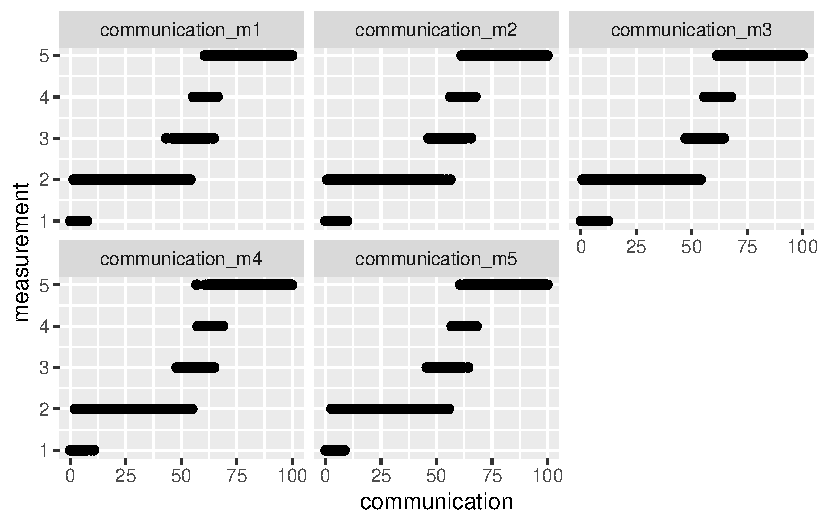
\includegraphics{./latent-variable-regression_files/figure-pdf/unnamed-chunk-5-1.pdf}

}

\end{figure}

\begin{Shaded}
\begin{Highlighting}[]
\NormalTok{model}\OtherTok{=}\StringTok{\textquotesingle{}communication \textasciitilde{} communication\_m1+communication\_m2+communication\_m3+communication\_m4+communication\_m5\textquotesingle{}}

\CommentTok{\# lavaan test}
\NormalTok{model.ord }\OtherTok{=} \FunctionTok{cfa}\NormalTok{(model, }\AttributeTok{data=}\NormalTok{dat }\SpecialCharTok{|\textgreater{}} \FunctionTok{rename}\NormalTok{(}\StringTok{"communication"} \OtherTok{=}\NormalTok{ communication), }\AttributeTok{ordered=}\FunctionTok{c}\NormalTok{(}
    \StringTok{"communication\_m1"}\NormalTok{,}
    \StringTok{"communication\_m2"}\NormalTok{,}
    \StringTok{"communication\_m3"}\NormalTok{,}
    \StringTok{"communication\_m4"}\NormalTok{,}
    \StringTok{"communication\_m5"}
\NormalTok{    )   }
\NormalTok{)}
\end{Highlighting}
\end{Shaded}

\begin{verbatim}
Warning in lav_data_full(data = data, group = group, cluster = cluster, : lavaan
WARNING: exogenous variable(s) declared as ordered in data: communication_m1
communication_m2 communication_m3 communication_m4 communication_m5
\end{verbatim}

\begin{verbatim}
Warning in lav_partable_check(lavpartable, categorical =
lavoptions$.categorical, : lavaan WARNING: parameter table does not contain
thresholds

Warning in lav_partable_check(lavpartable, categorical =
lavoptions$.categorical, : lavaan WARNING: parameter table does not contain
thresholds
\end{verbatim}

\begin{Shaded}
\begin{Highlighting}[]
\NormalTok{model.ord }\SpecialCharTok{|\textgreater{}} \FunctionTok{summary}\NormalTok{()}
\end{Highlighting}
\end{Shaded}

\begin{verbatim}
lavaan 0.6.16 ended normally after 18 iterations

  Estimator                                       DWLS
  Optimization method                           NLMINB
  Number of model parameters                         7

  Number of observations                         60000

Model Test User Model:
                                              Standard      Scaled
  Test Statistic                                 0.000       0.000
  Degrees of freedom                                 0           0

Parameter Estimates:

  Standard errors                           Robust.sem
  Information                                 Expected
  Information saturated (h1) model        Unstructured

Regressions:
                   Estimate  Std.Err  z-value  P(>|z|)
  communication ~                                     
    communicatn_m1    4.043    0.198   20.424    0.000
    communicatn_m2    3.517    0.201   17.509    0.000
    communicatn_m3    3.775    0.199   18.938    0.000
    communicatn_m4    3.852    0.202   19.081    0.000
    communicatn_m5    3.663    0.199   18.446    0.000

Intercepts:
                   Estimate  Std.Err  z-value  P(>|z|)
   .communication   -10.276    0.113  -91.324    0.000

Variances:
                   Estimate  Std.Err  z-value  P(>|z|)
   .communication   114.555    0.437  262.335    0.000
\end{verbatim}

Lastly, we'll simulate the outcome variables for survival analysis.
We'll use a Weibull likelihood. This is a popular choice for parametric
survival analysis because it can fit a pretty flexible monotonic
baseline hazard function, and can be interpretted as both a proportional
hazards and an acceleration failure time model, which gives us
flexibility in how we communicate results and frees us from the burden
of needing to check the proportional hazards assumption.

Could make it fancy by clustering people and doing it multilevel?

\begin{Shaded}
\begin{Highlighting}[]
\FunctionTok{clm}\NormalTok{(}\FunctionTok{factor}\NormalTok{(communication\_m1) }\SpecialCharTok{\textasciitilde{}}\NormalTok{ communication, }\AttributeTok{data =}\NormalTok{ dat)}
\end{Highlighting}
\end{Shaded}

\begin{verbatim}
formula: factor(communication_m1) ~ communication
data:    dat

 link  threshold nobs  logLik   AIC      niter max.grad cond.H 
 logit flexible  60000 -7952.06 15914.13 12(0) 7.10e-11 7.8e+06

Coefficients:
communication 
       0.9831 

Threshold coefficients:
   1|2    2|3    3|4    4|5 
 4.915 49.160 58.962 63.952 
\end{verbatim}

\begin{Shaded}
\begin{Highlighting}[]
\NormalTok{dat }\SpecialCharTok{|\textgreater{}} 

 \CommentTok{\#   filter(adaptability\_m1 \%in\% c(1, 2, 3)) |\textgreater{}}

    \FunctionTok{count}\NormalTok{(communication\_m1) }\SpecialCharTok{|\textgreater{}}

    \FunctionTok{mutate}\NormalTok{(}\AttributeTok{p =}\NormalTok{ n }\SpecialCharTok{/} \FunctionTok{sum}\NormalTok{(n))}
\end{Highlighting}
\end{Shaded}

\begin{verbatim}
# A tibble: 5 x 3
  communication_m1     n      p
             <dbl> <int>  <dbl>
1                1  3035 0.0506
2                2 27122 0.452 
3                3  5935 0.0989
4                4  2948 0.0491
5                5 20960 0.349 
\end{verbatim}

The idea is that if the latent variables predict time-to-employment then
that is consistent with them being well-measured, etc.

This example has closely mirrored an analysis I carried out for a real
client. In that example the latent variables had no predictive validity.

\hypertarget{prior-predictive-checks}{%
\section{Prior Predictive Checks}\label{prior-predictive-checks}}

\hypertarget{fitting-the-model}{%
\section{Fitting the Model}\label{fitting-the-model}}

\hypertarget{modelling-likert-measurements-as-ordinal-variables}{%
\section{Modelling Likert Measurements as Ordinal
Variables}\label{modelling-likert-measurements-as-ordinal-variables}}

We can improve the model.

\hypertarget{using-raw-stan-for-correlated-factors}{%
\section*{Using Raw STAN for Correlated
Factors}\label{using-raw-stan-for-correlated-factors}}
\addcontentsline{toc}{section}{Using Raw STAN for Correlated Factors}

\hypertarget{refs}{}
\begin{CSLReferences}{1}{0}
\leavevmode\vadjust pre{\hypertarget{ref-Green-et-al-1993}{}}%
al, Green et. n.d. {``Measurement Error Masks Bipolarity in Affect
Ratings.''} \emph{Journal of Personality and Social Psychology} 64(6).

\leavevmode\vadjust pre{\hypertarget{ref-Brilleman2020}{}}%
Brilleman, Samuel L., Eren M. Elci, Jacqueline Buros Novik, and Rory
Wolfe. 2020. {``Bayesian Survival Analysis Using the Rstanarm r
Package.''} \url{https://arxiv.org/abs/2002.09633}.

\leavevmode\vadjust pre{\hypertarget{ref-Brown2006}{}}%
Brown, Timothy A. 2006. \emph{Confirmatory Factor Analysis for Applied
Research}.

\leavevmode\vadjust pre{\hypertarget{ref-Collett2003}{}}%
Collett, David. 2003. \emph{Modelling Survival Data in Medical
Research}. 2nd ed. Chapman; Hall/CRC.

\leavevmode\vadjust pre{\hypertarget{ref-Finch2015}{}}%
Finch, French, W. Holmes. 2015. \emph{Latent Variable Modeling with r}.

\leavevmode\vadjust pre{\hypertarget{ref-Gelman2020}{}}%
Gelman, Andrew, Aki Vehtari, Daniel Simpson, Charles C. Margossian, Bob
Carpenter, Yuling Yao, Lauren Kennedy, Jonah Gabry, Paul-Christian
Bürkner, and Martin Modrák. 2020. {``Bayesian Workflow.''}
\url{https://arxiv.org/abs/2011.01808}.

\leavevmode\vadjust pre{\hypertarget{ref-gorsuch1983}{}}%
Gorsuch, Richard L. 1983. \emph{Factor Analysis, 2nd Edition}.

\leavevmode\vadjust pre{\hypertarget{ref-Kankaraux161-et-all-2019}{}}%
Kankaraš, Miloš, Eva Feron, and Rachel Renbarger. 2019. {``Assessing
Students' Social and Emotional Skills Through Triangulation of
Assessment Methods,''} no. 208.
https://doi.org/\url{https://doi.org/https://doi.org/10.1787/717ad7f2-en}.

\leavevmode\vadjust pre{\hypertarget{ref-Kline2011}{}}%
Kline, Rex B. 2011. \emph{Principles and Practice of Structural Equation
Modeling}.

\leavevmode\vadjust pre{\hypertarget{ref-McElreath2020}{}}%
McElreath, Richard; 2020. \emph{Statistical Rethinking: A Bayesian
Course with Examples in r and STAN}. 2nd ed. CRC Press LLC.

\leavevmode\vadjust pre{\hypertarget{ref-Singer+Willett2003}{}}%
Singer, Judith D., and John B. Willett. 2003. \emph{Applied Longitudinal
Data Analysis - Modeling Change and Event Occurrence}. Oxford University
Press.

\end{CSLReferences}



\end{document}
